\documentclass[11pt,a4paper]{article}

% ─── Packages ────────────────────────────────────────────────────────────────
\usepackage[utf8]{inputenc}
\usepackage[T1]{fontenc}
\usepackage{lmodern}
\usepackage{microtype}
\usepackage{geometry}
\usepackage{amsmath,amssymb,amsthm}
\usepackage{listings}
\usepackage{xcolor}
\usepackage{booktabs}
\usepackage{tabularx}
\usepackage{xltabular}
\usepackage{graphicx}
\usepackage{fancyhdr}
\usepackage{tikz}
\usetikzlibrary{arrows.meta,positioning,fit,backgrounds,calc,shapes.geometric,shapes.symbols,decorations.pathmorphing,decorations.pathreplacing}
\usepackage{float}
\usepackage{placeins}
\usepackage{caption}
\usepackage{enumitem}
\usepackage[backref=page]{hyperref}
\captionsetup{font=small,labelfont=bf}
% Algorithms are formatted using lstlisting with custom pseudocode style

% ─── Geometry ────────────────────────────────────────────────────────────────
\geometry{margin=2.5cm}

% ─── Colors ──────────────────────────────────────────────────────────────────
\definecolor{codebg}{RGB}{248,248,248}
\definecolor{codeframe}{RGB}{200,200,200}
\definecolor{darkgreen}{HTML}{00564C}
\definecolor{darkblue}{HTML}{003FB8}
\definecolor{accent}{HTML}{00564C}
\definecolor{hhsand}{HTML}{E9DCC4}
\definecolor{hhsanddeep}{HTML}{D8C7A6}
\definecolor{hhebony}{HTML}{121212}
\definecolor{hhink}{HTML}{1B1712}
\definecolor{hhcobalt}{HTML}{003FB8}
\definecolor{hhamber}{HTML}{6B4500}
\definecolor{hhteal}{HTML}{00564C}
\definecolor{hhpaper}{HTML}{FBF7EF}
\definecolor{hhgray}{HTML}{5C5650}
% The Book's semantic color system: palette v2, light values. One hue, one meaning.
% Source of record for every hex: website-v2/src/styles/tokens.semantic.css (light
% theme); website-v2/scripts/check-figure-palette.mjs fails the build if this file
% and the tokens disagree. Twin copy under book/figures/ (byte-identical).
%
% Separation: contrast says an ink is READABLE on the cream; it says nothing about
% whether two inks are TELLABLE APART, and until now only the first was checked.
% check-figure-palette-separation.mjs measures all 21 pairs in OKLab with protanopia
% and deuteranopia simulated. indigo and violet are re-stepped (deeper, on their own
% hues, both gaining contrast) because they were the pairs with room: cobalt/indigo
% was dE 9.1 and is 15.1; cobalt/violet collapsed to 4.8 under protanopia and is 8.6.
% Three pairs CANNOT be fixed -- teal/health, gold/health and teal/gold have ceilings
% of 12.2, 13.9 and 14.3 against a floor of 15, because sRGB has no chroma to spend
% on the 112-182 degree arc this dark. Only ONE of gold, health and teal may carry a
% series by colour alone; the others need a label, a gap, or a texture.
%
% Discipline: story colors are accents (rules, fills, marks, display text); body
% pages stay cream and ink. Amber is stripes, dots, and display only, never small
% text (3.71:1 on cream). Violet and gold are AA as text; use them at display size
% or on rules and fills. Line weights: 1px texture, 1.5px linework, 2px enclosure.
\definecolor{pdcobalt}{HTML}{003FB8}      % kernel / truth            --brand-primary
\definecolor{pdteal}{HTML}{006B5F}        % legibility                --brand-accent
\definecolor{pdhealth}{HTML}{1F7A4D}      % ready / coordinated       --story-health
\definecolor{pdindigo}{HTML}{312865}      % protocol / federation     --story-indigo
\definecolor{pdviolet}{HTML}{822586}      % identity / continuity     --story-violet
\definecolor{pdrust}{HTML}{7A4514}        % reputation / trust earned --story-rust
\definecolor{pdgold}{HTML}{666A00}        % economy / value           --story-gold
\definecolor{pdslate}{HTML}{384856}       % foundation / bedrock      --story-slate
\definecolor{pderror}{HTML}{BF2F2F}       % breach / correction       --status-error
\definecolor{pdamber}{HTML}{A66F00}       % warning (display only)    --status-warning
\definecolor{pdlime}{HTML}{CAD900}        % highlight fill, ink text  --chart-yellow
\definecolor{pdink}{HTML}{121212}         % ink                       --text-primary
\definecolor{pdinkmuted}{HTML}{403B34}    % links, secondary text     --text-secondary
\definecolor{pdcream}{HTML}{F2EEE6}       % page ground               --surface-base
\definecolor{pdcreamraised}{HTML}{F7F3EB} % panels                    --surface-raised
\definecolor{pdcreamstrong}{HTML}{E9E2D5} % inset wells               --surface-strong
% Print inks for the Swiss edition of the Book (SWISS-BRIEF, B); print only.
\definecolor{pdswissblue}{HTML}{001489}
\definecolor{pdswissviolet}{HTML}{582C83}
\definecolor{pdswissred}{HTML}{DA291C}
% And the maritime edition's fourth ink: antique gold, the trim of the engraved
% plates carried onto the page (opener rules, part-title ornament, fillets round
% framed matter). Flat stand-in for a metallic pass; print only.
\definecolor{pdmaritimegold}{HTML}{805A14}

\newcommand{\pdchapterprefix}{anchor}% this chapter's key in book/textbook.json
% GENERATED FILE. Do not edit by hand.
% Source of record: book/textbook.json (chapter order, numbers, parts, edition).
% Regenerate canonical map and site data: node scripts/generate-mega-whitepaper.mjs --sync-shared
% Drift check (CI): node --test scripts/generate-mega-whitepaper.test.mjs
% Canonical map: book/figures/pd-textbook-map.tex.
%
% Every standalone chapter preamble defines \pdchapterprefix before inputting
% this file; the Book redefines it at every \pdchapter. Everything else derives.

\providecommand{\pdeditiontitle}{Governing AI Agents: The Harbor, the Person, and the Economy}
\providecommand{\pdeditionsubtitle}{A Textbook of Concurrency, Identity, and Accountable Autonomous Work}
\providecommand{\pdeditionversion}{4.0 (Textbook Edition)}
\providecommand{\pdeditiondate}{5 November 2026}
\providecommand{\pdeditionclaim}{For autonomous work to remain accountable, each action needs an authority, a record, and someone responsible for its consequences.}
\providecommand{\pdbooktitle}{\emph{\pdeditiontitle}}
\providecommand{\pdchaptercount}{8}
\providecommand{\pdchaptercountword}{eight}
\providecommand{\pdpartcount}{4}
\providecommand{\pdchapterprefix}{none}
\expandafter\providecommand\csname pdchapternumberofnone\endcsname{0}
\expandafter\providecommand\csname pdchaptertitleofnone\endcsname{\pdeditiontitle}
\expandafter\providecommand\csname pdchaptercolorofnone\endcsname{pdcobalt}
\expandafter\providecommand\csname pdchapternumberofswk\endcsname{1}
\expandafter\providecommand\csname pdchaptertitleofswk\endcsname{The Single-Writer Kernel}
\expandafter\providecommand\csname pdchaptercolorofswk\endcsname{pdcobalt}
\expandafter\providecommand\csname pdchapterformerofswk\endcsname{II}
\expandafter\providecommand\csname pdchapterpartindexofswk\endcsname{1}
\expandafter\providecommand\csname pdchapterpartlabelofswk\endcsname{Part I \textperiodcentered\ Ground Truth}
\expandafter\providecommand\csname pdchapterquestionofswk\endcsname{Where can a rule be made real?}
\expandafter\providecommand\csname pdchapteronelineofswk\endcsname{A single program makes every change to a local database, one at a time; the chapter states which failures that record survives.}
\expandafter\providecommand\csname pdchapterepigraphofswk\endcsname{A transaction commits at the instant its commit record appears on disk.}
\expandafter\providecommand\csname pdchapterepigraphsourceofswk\endcsname{Jim Gray et al., The Recovery Manager of the System R Database Manager, 1981, p. 232}
\expandafter\providecommand\csname pdchapternumberofanchor\endcsname{2}
\expandafter\providecommand\csname pdchaptertitleofanchor\endcsname{The Anchor Protocol}
\expandafter\providecommand\csname pdchaptercolorofanchor\endcsname{pdcobalt}
\expandafter\providecommand\csname pdchapterformerofanchor\endcsname{V}
\expandafter\providecommand\csname pdchapterpartindexofanchor\endcsname{1}
\expandafter\providecommand\csname pdchapterpartlabelofanchor\endcsname{Part I \textperiodcentered\ Ground Truth}
\expandafter\providecommand\csname pdchapterquestionofanchor\endcsname{How may authority travel without silently growing?}
\expandafter\providecommand\csname pdchapteronelineofanchor\endcsname{When an agent passes a permission on, the new permission can only be narrower than the one it came from, at every step, and the checker verifies the whole chain.}
\expandafter\providecommand\csname pdchapterepigraphofanchor\endcsname{Every program and every user of the system should operate using the least set of privileges necessary to complete the job.}
\expandafter\providecommand\csname pdchapterepigraphsourceofanchor\endcsname{Jerome Saltzer and Michael Schroeder, The Protection of Information in Computer Systems, 1975}
\expandafter\providecommand\csname pdchapternumberofsealed\endcsname{3}
\expandafter\providecommand\csname pdchaptertitleofsealed\endcsname{The Sealed Harbor}
\expandafter\providecommand\csname pdchaptercolorofsealed\endcsname{pdcobalt}
\expandafter\providecommand\csname pdchapterformerofsealed\endcsname{}
\expandafter\providecommand\csname pdchapterpartindexofsealed\endcsname{1}
\expandafter\providecommand\csname pdchapterpartlabelofsealed\endcsname{Part I \textperiodcentered\ Ground Truth}
\expandafter\providecommand\csname pdchapterquestionofsealed\endcsname{What can a sealed agent leak, and how would we know?}
\expandafter\providecommand\csname pdchapteronelineofsealed\endcsname{A job run in a sealed environment can release results only through named checks, and all its releases together may disclose only a fixed amount of information, under the model's stated assumptions about channels.}
\expandafter\providecommand\csname pdchapterepigraphofsealed\endcsname{This note explores the problem of confining a program during its execution so that it cannot transmit information to any other program except its caller.}
\expandafter\providecommand\csname pdchapterepigraphsourceofsealed\endcsname{Butler W. Lampson, A Note on the Confinement Problem, 1973}
\expandafter\providecommand\csname pdchapternumberofls\endcsname{4}
\expandafter\providecommand\csname pdchaptertitleofls\endcsname{The Legible Swarm}
\expandafter\providecommand\csname pdchaptercolorofls\endcsname{pdteal}
\expandafter\providecommand\csname pdchapterformerofls\endcsname{I}
\expandafter\providecommand\csname pdchapterpartindexofls\endcsname{2}
\expandafter\providecommand\csname pdchapterpartlabelofls\endcsname{Part II \textperiodcentered\ The Cost of Seeing}
\expandafter\providecommand\csname pdchapterquestionofls\endcsname{What must remain visible, and what does seeing cost?}
\expandafter\providecommand\csname pdchapteronelineofls\endcsname{Useful supervision needs summaries that keep what the operator must decide on and link back to evidence the operator can inspect.}
\expandafter\providecommand\csname pdchapterepigraphofls\endcsname{In an information-rich world, the wealth of information means a dearth of something else: a scarcity of whatever it is that information consumes. What information consumes is rather obvious: it consumes the attention of its recipients.}
\expandafter\providecommand\csname pdchapterepigraphsourceofls\endcsname{Herbert A. Simon, Designing Organizations for an Information-Rich World, 1971}
\expandafter\providecommand\csname pdchapternumberofstp\endcsname{5}
\expandafter\providecommand\csname pdchaptertitleofstp\endcsname{From Spawn to Person}
\expandafter\providecommand\csname pdchaptercolorofstp\endcsname{pdviolet}
\expandafter\providecommand\csname pdchapterformerofstp\endcsname{III}
\expandafter\providecommand\csname pdchapterpartindexofstp\endcsname{3}
\expandafter\providecommand\csname pdchapterpartlabelofstp\endcsname{Part III \textperiodcentered\ What Survives the Restart}
\expandafter\providecommand\csname pdchapterquestionofstp\endcsname{What remains long enough to owe anything?}
\expandafter\providecommand\csname pdchapteronelineofstp\endcsname{An AI worker process starts, does a job and exits. Continuity links each replacement process, through a checked succession record, to one continuing account in a shared ledger, which shows what the worker owes, what it may do, which of its results an independent checker confirmed and which earlier processes it descends from. Reputation is what that record of confirmed results is worth to the next buyer.}
\expandafter\providecommand\csname pdchapterepigraphofstp\endcsname{We are but whirlpools in a river of ever-flowing water. We are not stuff that abides, but patterns that perpetuate themselves.}
\expandafter\providecommand\csname pdchapterepigraphsourceofstp\endcsname{Norbert Wiener, The Human Use of Human Beings: Cybernetics and Society, revised edition, 1954}
\expandafter\providecommand\csname pdchapternumberofhe\endcsname{6}
\expandafter\providecommand\csname pdchaptertitleofhe\endcsname{The Harbor Economy}
\expandafter\providecommand\csname pdchaptercolorofhe\endcsname{pdgold}
\expandafter\providecommand\csname pdchapterformerofhe\endcsname{IV}
\expandafter\providecommand\csname pdchapterpartindexofhe\endcsname{4}
\expandafter\providecommand\csname pdchapterpartlabelofhe\endcsname{Part IV \textperiodcentered\ Trade Between Strangers}
\expandafter\providecommand\csname pdchapterquestionofhe\endcsname{What makes cooperation rational without making loss unbounded?}
\expandafter\providecommand\csname pdchapteronelineofhe\endcsname{Labor, rented assets and licensed skills carry different risks, but all of them settle through one shared ledger in which no transfer creates or destroys any unit of payment.}
\expandafter\providecommand\csname pdchapterepigraphofhe\endcsname{The main reason why it is profitable to establish a firm would seem to be that there is a cost of using the price mechanism.}
\expandafter\providecommand\csname pdchapterepigraphsourceofhe\endcsname{Ronald H. Coase, The Nature of the Firm, 1937}
\expandafter\providecommand\csname pdchapternumberofbonded\endcsname{7}
\expandafter\providecommand\csname pdchaptertitleofbonded\endcsname{The Bonded Commons}
\expandafter\providecommand\csname pdchaptercolorofbonded\endcsname{pdgold}
\expandafter\providecommand\csname pdchapterformerofbonded\endcsname{VI}
\expandafter\providecommand\csname pdchapterpartindexofbonded\endcsname{4}
\expandafter\providecommand\csname pdchapterpartlabelofbonded\endcsname{Part IV \textperiodcentered\ Trade Between Strangers}
\expandafter\providecommand\csname pdchapterquestionofbonded\endcsname{Who may decide, on what evidence, with what consequence?}
\expandafter\providecommand\csname pdchapteronelineofbonded\endcsname{Some doubt about an agent's work remains even after access checks. The chapter handles it with shared rules: providers post deposits (bonds), signed records show who did what, audits sample the results, and either side can appeal a verdict. A model checker confirms, on a bounded model, that the deposit ledger never creates or loses money.}
\expandafter\providecommand\csname pdchapterepigraphofbonded\endcsname{The power to constrain an adversary may depend on the power to bind oneself.}
\expandafter\providecommand\csname pdchapterepigraphsourceofbonded\endcsname{Thomas C. Schelling, The Strategy of Conflict, 1960}
\expandafter\providecommand\csname pdchapternumberoffh\endcsname{8}
\expandafter\providecommand\csname pdchaptertitleoffh\endcsname{The Federated Harbor}
\expandafter\providecommand\csname pdchaptercoloroffh\endcsname{pdgold}
\expandafter\providecommand\csname pdchapterformeroffh\endcsname{VII}
\expandafter\providecommand\csname pdchapterpartindexoffh\endcsname{4}
\expandafter\providecommand\csname pdchapterpartlabeloffh\endcsname{Part IV \textperiodcentered\ Trade Between Strangers}
\expandafter\providecommand\csname pdchapterquestionoffh\endcsname{What can cross a trust boundary without moving the authority itself?}
\expandafter\providecommand\csname pdchapteronelineoffh\endcsname{Machines run by owners who do not trust each other can pass each other signed records, but not the power to approve actions on each other's systems. The chapter works out which information can spread from machine to machine, which decisions still need one designated approver, and why the receiving machine must issue its own permission for its own resources instead of narrowing the sender's.}
\expandafter\providecommand\csname pdchapterepigraphoffh\endcsname{We reject: kings, presidents and voting. We believe in: rough consensus and running code.}
\expandafter\providecommand\csname pdchapterepigraphsourceoffh\endcsname{David D. Clark, A Cloudy Crystal Ball: Visions of the Future, 1992}
\providecommand{\pdchapternumber}{\csname pdchapternumberof\pdchapterprefix\endcsname}
\providecommand{\pdchaptertitle}{\csname pdchaptertitleof\pdchapterprefix\endcsname}
\providecommand{\pdchaptercolor}{\csname pdchaptercolorof\pdchapterprefix\endcsname}
\providecommand{\pdchapterpartindex}{\csname pdchapterpartindexof\pdchapterprefix\endcsname}
\providecommand{\pdchapterpartlabel}{\csname pdchapterpartlabelof\pdchapterprefix\endcsname}
\providecommand{\pdchapterquestion}{\csname pdchapterquestionof\pdchapterprefix\endcsname}
\providecommand{\pdchapteroneline}{\csname pdchapteronelineof\pdchapterprefix\endcsname}
\providecommand{\pdchapterepigraph}{\csname pdchapterepigraphof\pdchapterprefix\endcsname}
\providecommand{\pdchapterepigraphsource}{\csname pdchapterepigraphsourceof\pdchapterprefix\endcsname}

% Parts, for the weighted four-hue rule: numeral, hue, the label that ends the
% part (the next part, or the appendices), and the chapter count used as the
% weight until page references exist. \pdweightrule (Book preamble) consumes it.
\providecommand{\pdfirstpartnumeral}{I}
\providecommand{\pdweightsegmentslist}{%
  \pdweightsegment{I}{pdcobalt}{part:II}{3}%
  \pdweightsegment{II}{pdteal}{part:III}{1}%
  \pdweightsegment{III}{pdviolet}{part:IV}{1}%
  \pdweightsegment{IV}{pdgold}{book:appendices}{3}%
}
\expandafter\providecommand\csname pdpartindexofI\endcsname{1}
\expandafter\providecommand\csname pdpartindexofII\endcsname{2}
\expandafter\providecommand\csname pdpartindexofIII\endcsname{3}
\expandafter\providecommand\csname pdpartindexofIV\endcsname{4}
\expandafter\providecommand\csname pdparttitleofI\endcsname{Ground Truth}
\expandafter\providecommand\csname pdparttitleofII\endcsname{The Cost of Seeing}
\expandafter\providecommand\csname pdparttitleofIII\endcsname{What Survives the Restart}
\expandafter\providecommand\csname pdparttitleofIV\endcsname{Trade Between Strangers}

% Locator map: every part and chapter of the Book, the current chapter marked.
% \pdchaplink is provided by figures/pd-hyperlinks.tex (a live link inside the
% Book, plain text in a standalone chapter).
\providecommand{\pdmapchapter}[3]{%
  \ifnum#1=\pdchapternumber\relax
    \textbf{\pdchaplink{#2}{#1.~#3}}~\textnormal{(this chapter)}%
  \else
    \pdchaplink{#2}{#1.~#3}%
  \fi}
\providecommand{\pdtextbookmap}{%
  \begin{tabular}{@{}l@{\quad}p{\dimexpr\linewidth-12em\relax}@{}}
  \textsc{\textbf{Part I}}\ Ground Truth & \raggedright \pdmapchapter{1}{swk}{The Single-Writer Kernel} \textperiodcentered\ \pdmapchapter{2}{anchor}{The Anchor Protocol} \textperiodcentered\ \pdmapchapter{3}{sealed}{The Sealed Harbor}\tabularnewline[2pt]
  \textsc{\textbf{Part II}}\ The Cost of Seeing & \raggedright \pdmapchapter{4}{ls}{The Legible Swarm}\tabularnewline[2pt]
  \textsc{\textbf{Part III}}\ What Survives the Restart & \raggedright \pdmapchapter{5}{stp}{From Spawn to Person}\tabularnewline[2pt]
  \textsc{\textbf{Part IV}}\ Trade Between Strangers & \raggedright \pdmapchapter{6}{he}{The Harbor Economy} \textperiodcentered\ \pdmapchapter{7}{bonded}{The Bonded Commons} \textperiodcentered\ \pdmapchapter{8}{fh}{The Federated Harbor}\tabularnewline[2pt]
  \end{tabular}}

% Shared pedagogic apparatus for the Book and every standalone chapter: boxed
% claims, honest boundaries, worked examples, retrieval prompts, numbered
% exercises, and their deferred solutions.
% Twin copy under book/figures/ (byte-identical; checked by
% scripts/generate-mega-whitepaper.test.mjs).
%
% \input this immediately after figures/pd-textbook-map (so \pdchapterprefix
% and \pdchapternumber already resolve) and before figures/pd-hyperlinks.
%
% Page grammar (Wave 12): a content kind is signalled by typography and the
% margin, never by a tinted rectangle. Claims: a hairline above, a small-caps
% run-in head, a short hairline below. Worked examples: two hairlines and an
% italic head. Boundaries: a plain ink bar at the left, no fill. Recitation:
% margin prompts in the Book, a compact list in a standalone chapter.
% Exercises: a numbered hanging paragraph with kind and stars in small caps,
% the solution page in the margin. Nothing here paints a background.
%
% \ifpdmargincolumn is false by default (standalone A4 chapters have no margin
% column); the Book's preamble sets \pdmargincolumntrue after its geometry.
% mdframed is used only for the bars (leftline) and hairlines (top/bottom),
% with the DEFAULT frame method -- never framemethod=tikz.
%
% Key-value parsing for \pdexercise uses pgfkeys: pgf ships as part of tikz,
% which every preamble already loads, so this adds no new dependency (keyval
% would have meant one). The closed kind/rating vocabularies are enforced with
% the LaTeX kernel's own \in@/\ifin@ comma-list test -- always available,
% no package of its own -- wrapped in an \edef that expands both sides first:
% \in@ does not expand its own arguments, so hunting for a *macro* (rather
% than literal text) requires pre-expanding it, or every kind reads as absent.
\makeatletter
\@ifpackageloaded{mdframed}{}{\usepackage{mdframed}}
\@ifpackageloaded{answers}{}{\usepackage{answers}}
\@ifpackageloaded{marginnote}{}{\usepackage{marginnote}}
\@ifpackageloaded{environ}{}{\usepackage{environ}}
\@ifpackageloaded{etoolbox}{}{\usepackage{etoolbox}}
\@ifpackageloaded{listings}{}{\usepackage{listings}}
\@ifpackageloaded{caption}{}{\usepackage{caption}}
\@ifpackageloaded{tcolorbox}{}{\usepackage[skins,breakable,listings]{tcolorbox}}

% ---------------------------------------------------------------------------
% Shared helpers: the margin-column switch, the margin head, the margin glyph.
% ---------------------------------------------------------------------------
% The Book defines \pdcurrentchaptercolor (per part) AFTER this file; a
% standalone chapter never does. Resolve it lazily, falling back to cobalt.
\newcommand{\pd@chaptercolor}{\ifdefined\pdcurrentchaptercolor\pdcurrentchaptercolor\else pdcobalt\fi}
% The eight standalone chapter PDFs this false branch exists for are retired
% as of this change (the chapters no longer build or publish an A4 edition of
% themselves). Every \ifpdmargincolumn false branch below is now dead weight
% kept alive only by the chapters' .tex sources still being independently
% compilable; do NOT delete it in this change -- the margin apparatus work is
% in flight on another branch and this would collide with it. Removing the
% false branch (and, eventually, the conditional itself) is that wave's job.
\newif\ifpdmargincolumn
\pdmargincolumnfalse
% The Book overrides this with an unnumbered, baseline-aligned margin aside.
% Keep chapter sources independently compilable without duplicating prose.
\providecommand{\pdsourceaside}[1]{\footnote{#1}}
% An intentional body boundary: flush pending figures before a new margin
% discussion. The generator strips legacy literal chapter-opening breaks,
% but preserves this explicit editorial instruction. Never use it in frames.
\newcommand{\pdmarginpagebreak}{\clearpage}
\renewcommand*{\marginfont}{\footnotesize\raggedright\color{pdinkmuted}}
% A small-caps head: set in the margin when the Book has a margin column,
% otherwise run in at the start of the paragraph.
% A head stays a \marginnote, and the reason is worth keeping. It was set as
% a \marginpar for one build (2026-09-08), so the page builder would keep the
% Recall block clear of it, and the build died with "Float(s) lost" at the end
% of chapter 1. \ifinner is true inside a minipage or mdframed only BETWEEN
% paragraphs; the moment a paragraph starts it is ordinary horizontal mode,
% \ifinner is false, and a \marginpar issued there -- a \keyidea inside a
% pdexample -- has no page to be shipped to. The heads are one line each and
% are never what runs into something; the Recall block was, and it is now a
% \marginpar issued in vertical mode, where the test is honest.
% Each head records the page and the page-height at which it was issued, so a
% Recall block raised later on the same page can stop short of it. A head is
% issued at the start of its paragraph, where \pagetotal is the page above the
% paragraph -- the head's own position, to within a line.
% Margin occupancy is tracked both ways. A head records where it was issued
% so a Recall block raised later on the page stops short of it; a Recall block
% records where its foot came to rest so a head issued later on the same page
% (the next section's first Key idea) steps down below it instead of printing
% inside it. \pagetotal at a head lags by the current paragraph, which puts
% every error on the safe side: the block is capped a little low, the head
% steps a little far.
\def\pd@lastheadpage{0}\newlength{\pd@lastheadbottom}
\def\pd@blockpage{0}\newlength{\pd@blockbottom}\newlength{\pd@headshift}
\newsavebox{\pd@headbox}\newsavebox{\pd@ptrbox}\newsavebox{\pd@sidebox}
% Run the page builder so \pagetotal counts the paragraph that just ended.
% Without it \pagetotal is the page above the LAST paragraph the builder saw,
% which under-reads by however much prose has since been set -- and every
% device here decides where it may sit from that number. A Boundary head read
% a stale \pagetotal and recorded its foot a paragraph too high, and the Recall
% block that followed cleared that phantom and printed on the head itself
% (0.1 pt apart on p. 253 of the technical edition). \penalty\@M contributes
% without opening a breakpoint. Outer vertical mode only: inside a box the
% penalty lands on the box's own list and settles nothing.
\newcommand{\pd@settle}{\ifvmode\ifinner\else\penalty\@M\vskip\z@\fi\fi}
% ---------------------------------------------------------------------------
% Figure-band tracking, for vertical CENTERING of a margin device against the
% main-column figure it accompanies (2026-09). \pd@figtop/\pd@figbot/\pd@figpage
% are declared here but SET in the Book preamble's \pgfsys@typesetpicturebox
% hook (coordination-papers-mega-volume-preamble.tex), not by an
% \AtBeginEnvironment{figure}/\AtEndEnvironment{figure} pair on \pagetotal --
% that was the first attempt and it does not work: for a \begin{figure}[H]
% float, the `float' package defers inserting the box into the main vertical
% list past \end{figure} itself, so \pagetotal read there under-reads by the
% whole figure and \pd@figbot always came out equal to \pd@figtop (measured:
% every firing in the built Book). The pgf hook that already intercepts every
% TikZ picture on its way into the page knows the box's own \ht+\dp directly,
% which is exact regardless of page-builder timing, so that is where the span
% is recorded now. \pd@figpage guards against reading a stale span left over
% from a figure several pages back: \pd@placemargin only trusts the span when
% \pd@figpage still equals the numeric page counter. Only one span is kept -- the most
% recently drawn picture on this page -- which is deliberately the figure a
% margin device issued shortly afterward is almost always about; a page with
% two unrelated figures and one margin device between them is not a case this
% file has seen.
\newlength{\pd@figtop}\newlength{\pd@figbot}\def\pd@figpage{0}
% Does OFFSET (already sitting in \pd@blockoff) sit inside the room this page
% actually has for it, without moving? \pd@reqmin/\pd@reqmax are computed by
% \pd@marginbounds below, from exactly the three collision facts \pd@placemargin
% already knew about (page top, the last margin head, the last margin block) --
% this is a read of the same facts, not a new rule. A candidate that fits
% clean is preferred over one merely clamped INTO range, because a clamped
% value is a collision this page already had; a candidate the bounds do not
% touch is one that was never in anyone's way.
\newlength{\pd@reqmin}\newlength{\pd@reqmax}\newif\ifpd@havemax\newif\ifpd@fits
\newcommand{\pd@marginbounds}[1]{%
  \setlength{\pd@reqmin}{-\pagetotal}%
  \ifnum\pd@lastheadpage=\value{page}\relax
    \ifdim\pd@reqmin<\dimexpr\pd@lastheadbottom-\pagetotal\relax
      \setlength{\pd@reqmin}{\dimexpr\pd@lastheadbottom-\pagetotal\relax}\fi\fi
  \ifnum\pd@blockpage=\value{page}\relax
    \ifdim\pd@reqmin<\dimexpr\pd@blockbottom-\pagetotal+2pt\relax
      \setlength{\pd@reqmin}{\dimexpr\pd@blockbottom-\pagetotal+2pt\relax}\fi\fi
  \ifdim\pagegoal<\maxdimen
    \pd@havemaxtrue
    \setlength{\pd@reqmax}{\dimexpr\pagegoal-\pagetotal-\ht#1-\dp#1\relax}%
  \else\pd@havemaxfalse\fi}
\newcommand{\pd@tryoffset}{%
  \pd@fitstrue
  \ifdim\pd@blockoff<\pd@reqmin\pd@fitsfalse\fi
  \ifpd@fits\ifpd@havemax\ifdim\pd@blockoff>\pd@reqmax\pd@fitsfalse\fi\fi\fi}
\newcommand{\pd@marginhead}[1]{%
  \ifpdmargincolumn
    % Settle before the first \pagetotal read, unlike this macro's earlier
    % form. Every OTHER margin device in this file settles first (the
    % comment two macros up even says why: "\pagetotal is the page above
    % the LAST paragraph the builder saw"), but this one read \pagetotal
    % raw at the head's own issuing point and called the resulting slop
    % "to within a line" -- acceptable when a block follows a head closely,
    % not when many lines of prose come between them and a margin block
    % later clamps to \pd@lastheadbottom expecting it exact. Measured: a
    % \pdboundary head ("Where this stops") 14 lines above its section's
    % \end{pdrecitation}, recorded 2.35 pt short, so the Recall block's
    % clamp (aimed at a 3 pt gap under the head) landed 2.35 pt INSIDE it
    % instead -- built and measured overlapping, PDF p. 244.
    \pd@settle
    \setlength{\pd@headshift}{0pt}%
    \ifnum\pd@blockpage=\value{page}\relax
      \ifdim\pagetotal<\pd@blockbottom
        \setlength{\pd@headshift}{\dimexpr\pd@blockbottom-\pagetotal+3pt\relax}\fi
    \fi
    % And around the last HEAD on this page, which this macro recorded below
    % and then never read. Blocks stepped around heads, heads stepped around
    % blocks, and two heads walked straight through each other: a Pitfall head
    % printed 1.0 pt from a Recall head at the top of p. 306 of the maritime
    % edition, inside the 10.4 pt leading the collision check measures. The
    % rule is the same one \pd@placemargin already obeys three lines at a
    % time -- never above what is already in the column -- so it is applied
    % here in the same shape, after the block cap so whichever foot sits
    % lower wins.
    \ifnum\pd@lastheadpage=\value{page}\relax
      \ifdim\dimexpr\pagetotal+\pd@headshift\relax<\pd@lastheadbottom
        \setlength{\pd@headshift}{\dimexpr\pd@lastheadbottom-\pagetotal+3pt\relax}\fi
    \fi
    % A twin of the head, set at the margin's width and font, measured but
    % never shipped: a head of three or four words wraps to two lines there,
    % and a block raised later on the page has to clear the head's real foot.
    % Assuming one line put "RECALL" 0.1 pt under "WHERE THIS STOPS" in the
    % Swiss and technical editions, whose pagination differs from the
    % maritime edition's by a page.
    \sbox{\pd@headbox}{\begin{minipage}{\marginparwidth}\marginfont\scshape #1\end{minipage}}%
    \marginnote{\scshape #1}[\pd@headshift]%
    \xdef\pd@lastheadpage{\number\value{page}}%
    % +8pt, not +3pt: \pd@headbox measures the head's own text, but the
    % marginnote package sets every note's content behind a \strut (its
    % \marginfont\raggedrightmarginnote\strut...) whose height+depth come
    % from \marginfont's normal font metrics, not from \scshape "Where this
    % stops" alone -- the strut is measurably taller, so \ht+\dp here
    % under-reads the head's true rendered bottom. +3pt covered one 0.1pt
    % case (comment above); it did not cover this one -- built and measured
    % a Recall block clamped to +3pt still overlapping "Where this stops" by
    % 2.35 pt (PDF p. 244, pdboundary fourteen lines above its section's
    % \end{pdrecitation}). +8pt re-measured clear on that page and does not
    % reopen the "1.3 pt under" case the \newpage reservation above already
    % handles (a different mechanism -- a migrated page, not a short strut).
    \global\pd@lastheadbottom=\dimexpr\pagetotal+\pd@headshift
      +\ht\pd@headbox+\dp\pd@headbox+8pt\relax
  \else{\scshape #1.}\enspace\fi}
% A small square in the chapter's hue, in the margin, marking a worked example
% so a reader flipping through finds every one.
\newlength{\pd@blockoff}
% Place a measured margin block so its LAST line sits on the line that issues
% it -- the block occupies the page above its anchor rather than hanging below
% it, which is what keeps a note issued near the foot on the paper at all.
% Three caps, in order: never above the page top; never above the last margin
% head on this page (measured to that head's own foot); never above the last
% block on this page. Then the block records where its foot came to rest, so a
% head issued later steps down below it. \pagetotal is the shared clock for all
% of this, which is why every device that can settles the page builder first.
% Every margin device goes through here, including the three the margin
% apparatus added (\pdcite, \pdprov, \pdprovedon): a device that places its
% own note without asking what is already in the column is how the Book got
% seven collisions and a portrait below the paper, and there are now several
% hundred short notes in the column where there were dozens.
% Place a margin block with its TOP on the issuing line rather than its foot.
% Same occupancy bookkeeping as \pd@placemargin -- it must, or a later block
% would be told the column is free where this one sits -- but it never raises,
% so it cannot leave the page above. Clamped both ways: the offset is never
% negative (nothing above the text block) and, where \pagegoal is a real
% dimension, never so large that the block's foot passes the bottom of the
% text block. \pagegoal is \maxdimen on an empty page, which is room for
% anything; a block already taller than its page is left alone rather than
% shoved, because moving it cannot make it fit.
\newlength{\pd@blockfloor}
\newcommand{\pd@placemargintop}[1]{%
  \setlength{\pd@blockoff}{0pt}%
  \ifnum\pd@lastheadpage=\value{page}\relax
    \ifdim\pd@blockoff<\dimexpr\pd@lastheadbottom-\pagetotal\relax
      \setlength{\pd@blockoff}{\dimexpr\pd@lastheadbottom-\pagetotal\relax}\fi
  \fi
  \ifnum\pd@blockpage=\value{page}\relax
    \ifdim\pd@blockoff<\dimexpr\pd@blockbottom-\pagetotal+2pt\relax
      \setlength{\pd@blockoff}{\dimexpr\pd@blockbottom-\pagetotal+2pt\relax}\fi
  \fi
  \ifdim\pd@blockoff<0pt \setlength{\pd@blockoff}{0pt}\fi
  % The floor the two caps above just established: whatever is already in the
  % column on this page ends here, and nothing may be placed above it.
  \setlength{\pd@blockfloor}{\pd@blockoff}%
  % Pull the block up if its foot would pass the bottom of the text block --
  % but never above that floor. Reducing the offset past it is how the
  % foot-anchored placement used to undo its own downward pushes: a clamp
  % applied last re-collides the block with the head or the note it was just
  % moved clear of, which is the defect this file's other comment records as
  % 132 collisions on one merge. A block too tall to satisfy both is left at
  % the floor and overruns the foot, where page_overflow.py's foot-intrusion
  % and off-the-paper checks will report it -- a visible, measured overrun is
  % worth more than a silent overlap.
  \ifdim\pagegoal<\maxdimen
    \ifdim\dimexpr\pagetotal+\pd@blockoff+\ht#1+\dp#1\relax>\pagegoal
      \setlength{\pd@blockoff}{\dimexpr\pagegoal-\pagetotal-\ht#1-\dp#1\relax}%
      \ifdim\pd@blockoff<\pd@blockfloor \setlength{\pd@blockoff}{\pd@blockfloor}\fi
    \fi
  \fi
  \marginnote{\usebox#1}[\pd@blockoff]%
  \xdef\pd@blockpage{\number\value{page}}%
  \global\pd@blockbottom=\dimexpr\pagetotal+\pd@blockoff+\ht#1+\dp#1\relax}

% Default placement is now CENTERED on the vertical span of the most recently
% closed figure on this page, not anchored to the line that issues the note --
% a Recall block or a gloss discussing a figure reads naturally beside its
% middle, not hanging off one edge. Center only WHEN IT FITS CLEAN: tried
% against \pd@marginbounds's read of the same three collision facts the old
% single anchor already obeyed (page top, the last margin head, the last
% margin block), with no clamping. A center that does not fit clean is not
% clamped into place -- clamping a center is neither center nor top nor
% bottom, it is just wherever the clamp landed, and the point of asking for an
% aligned center was to get one honestly or not at all. Top-of-figure is tried
% next, then bottom-of-figure; the first of the three that needs no clamp
% wins. If none does, this falls through unchanged to the pre-existing
% issuing-line anchor and its own clamps below -- the same fallback this file
% always had, now reached only when no figure-relative placement clears.
\newif\ifpd@figcentered
\newcommand{\pd@placemargin}[1]{%
  \pd@figcenteredfalse
  \ifnum\pd@figpage=\value{page}\relax\ifdim\pd@figbot>\z@
    \pd@marginbounds{#1}%
    \setlength{\pd@blockoff}{\dimexpr(\pd@figtop+\pd@figbot)/2-\pagetotal-(\ht#1+\dp#1)/2\relax}%
    \pd@tryoffset
    \ifpd@fits\pd@figcenteredtrue\else
      \setlength{\pd@blockoff}{\dimexpr\pd@figtop-\pagetotal\relax}%
      \pd@tryoffset
      \ifpd@fits\pd@figcenteredtrue\else
        \setlength{\pd@blockoff}{\dimexpr\pd@figbot-\pagetotal-\ht#1-\dp#1\relax}%
        \pd@tryoffset
        \ifpd@fits\pd@figcenteredtrue\fi
      \fi
    \fi
  \fi\fi
  \ifpd@figcentered
    \marginnote{\usebox#1}[\pd@blockoff]%
    \xdef\pd@blockpage{\number\value{page}}%
    \global\pd@blockbottom=\dimexpr\pagetotal+\pd@blockoff+\ht#1+\dp#1\relax
  \else
  \setlength{\pd@blockoff}{\dimexpr\baselineskip-\ht#1-\dp#1\relax}%
  % A note never starts below the line that issues it -- clamped here, BEFORE
  % the occupancy caps, not after. Clamping last undid every downward push:
  % two \pdcite calls in one paragraph read the same \pagetotal, so the second
  % was told to start below the first's foot and then clamped straight back
  % onto it (132 collisions on the merge, all of them pairs of citations on
  % one line). Below the anchor is exactly where a second note belongs.
  \ifdim\pd@blockoff>0pt \setlength{\pd@blockoff}{0pt}\fi
  \ifdim\pd@blockoff<-\pagetotal
    \setlength{\pd@blockoff}{-\pagetotal}%
    % Headroom at the column top, and the reason is the one hole left in the
    % occupancy model. Every cap below is keyed on the numeric page counter, which is the
    % page the device was ISSUED on -- and a head issued in the last line of
    % a page whose paragraph then breaks prints at the top of the NEXT page
    % while having recorded the page before. That is exactly the Recall-on-
    % Pitfall collision at the top of p. 306 of the maritime edition: the
    % Pitfall head began its paragraph at the foot of p. 305, migrated with
    % the break, and the Recall block clamped flush to p. 306's column top
    % and landed 1.0 pt from a head no cap could see. TeX cannot tell us the
    % shipout page here, so the fix is not a better cap but a reservation:
    % when the top clamp binds, leave two lines for whatever may have come
    % over the break. Two, not one, because a head of three or four words
    % wraps to two lines at the margin's width. Only when there is room --
    % \pagegoal is \maxdimen on an empty page, which is room enough for
    % anything, and a block already too tall for its page is left where the
    % clamp put it rather than pushed off the paper.
    \ifdim\dimexpr\pagetotal+\pd@blockoff+2\baselineskip+\ht#1+\dp#1\relax>\pagegoal
      \ifdim\dimexpr\pagetotal+\pd@blockoff+\baselineskip+\ht#1+\dp#1\relax>\pagegoal
      \else\setlength{\pd@blockoff}{\dimexpr\pd@blockoff+\baselineskip\relax}\fi
    \else\setlength{\pd@blockoff}{\dimexpr\pd@blockoff+2\baselineskip\relax}\fi
  \fi
  \ifnum\pd@lastheadpage=\value{page}\relax
    \ifdim\pd@blockoff<\dimexpr\pd@lastheadbottom-\pagetotal\relax
      \setlength{\pd@blockoff}{\dimexpr\pd@lastheadbottom-\pagetotal\relax}\fi
  \fi
  \ifnum\pd@blockpage=\value{page}\relax
    \ifdim\pd@blockoff<\dimexpr\pd@blockbottom-\pagetotal+2pt\relax
      \setlength{\pd@blockoff}{\dimexpr\pd@blockbottom-\pagetotal+2pt\relax}\fi
  \fi
  \marginnote{\usebox#1}[\pd@blockoff]%
  \xdef\pd@blockpage{\number\value{page}}%
  \global\pd@blockbottom=\dimexpr\pagetotal+\pd@blockoff+\ht#1+\dp#1\relax
  \fi}
% The same placement for a note the page can do without. A Recall block, a
% margin figure and a gloss carry content that is nowhere else, so they are
% always placed. A short-form citation, a provenance note and a discharge
% pointer are second copies: \pdcite has already emitted the \cite, so the
% work is in the text and in the bibliography whatever the margin does. There
% are several hundred of them and on a dense page the column has no room for
% one beside every line that cites -- arithmetic cannot make space that is not
% there. So when placing one would push its foot past the text block's foot,
% it is left out rather than printed over its neighbour or below the paper.
% Nothing is lost that a reader could otherwise have read.
\newcommand{\pd@placemarginopt}[1]{%
  \setlength{\pd@blockoff}{\dimexpr\baselineskip-\ht#1-\dp#1\relax}%
  \ifdim\pd@blockoff>0pt \setlength{\pd@blockoff}{0pt}\fi
  \ifdim\pd@blockoff<-\pagetotal \setlength{\pd@blockoff}{-\pagetotal}\fi
  \ifnum\pd@lastheadpage=\value{page}\relax
    \ifdim\pd@blockoff<\dimexpr\pd@lastheadbottom-\pagetotal\relax
      \setlength{\pd@blockoff}{\dimexpr\pd@lastheadbottom-\pagetotal\relax}\fi
  \fi
  \ifnum\pd@blockpage=\value{page}\relax
    \ifdim\pd@blockoff<\dimexpr\pd@blockbottom-\pagetotal+2pt\relax
      \setlength{\pd@blockoff}{\dimexpr\pd@blockbottom-\pagetotal+2pt\relax}\fi
  \fi
  % Room left on this page, measured to the block's foot, with two lines of
  % slack. \pagegoal is \maxdimen while the page is empty, which is room
  % enough for anything. The slack is there because \pagetotal under-reads
  % mid-paragraph, which is where most of these are called: without it the
  % guard believed there was room and put an Exercises pointer 8.2 pt off the
  % foot of p. 309 of the Swiss edition -- a page that only exists in the CI
  % build's pagination, which is why the local builds were clean and the check
  % running over every edition in CI is what found it.
  \ifdim\dimexpr\pagetotal+\pd@blockoff+\ht#1+\dp#1+2\baselineskip\relax>\pagegoal
  \else
    \marginnote{\usebox#1}[\pd@blockoff]%
    \xdef\pd@blockpage{\number\value{page}}%
    \global\pd@blockbottom=\dimexpr\pagetotal+\pd@blockoff+\ht#1+\dp#1\relax
  \fi}
\newcommand{\pd@marginglyph}{%
  \ifpdmargincolumn\marginnote{\textcolor{\pd@chaptercolor}{\rule[-0.5pt]{4.5pt}{4.5pt}}}\fi}

% \pdgloss{Term}{one-line definition} -- a defined term set bold where it is
% defined, in the running text, the way the Book already sets any term of art
% at its point of definition; the definition itself is carried as a margin
% note rather than left inline, so a reader can recall it from the margin
% without re-parsing the sentence. In the margin column (Book) this reuses
% the small-caps head convention \pd@marginhead sets for \keyidea, \pitfall
% and \xrefbox's own heads, but folds head and body into ONE \marginnote call
% -- calling \pd@marginhead and a separate \marginnote back to back would
% place two independent margin boxes at the same source line and risk them
% colliding, exactly what \pdmarginfigure avoids by building one combined box
% for its image and caption. The margin text renders at \marginfont, the
% same footnotesize sidenote size every other margin note in this file uses.
% Outside the margin column (standalone chapters) the definition folds back
% into the sentence as a parenthetical, so no content is lost. No box, no
% rule -- a bare labelled aside like every other device here. No trailing
% \ignorespaces: unlike \pdboundary/\pdexample (environments whose content
% starts on the next source line), \pdgloss is called mid-sentence and the
% genuine word space that follows it in the prose must survive.
% The note is measured and RAISED so its last line sits on the line that
% issues it, for the same reason the Recall block is: a gloss called in the
% last line or two of a page hung its definition below the paper, where the
% log says nothing and the reader has nothing (Lamport's gloss, 81 pt off the
% foot of p. 68 in the technical edition). Raised, the note occupies the page
% above its anchor, which is page the anchor is on by construction; the only
% cap it needs is the page top. \pagetotal is read mid-sentence here and so
% lags by the lines of the current paragraph -- it under-reads, so the top cap
% fires a little early and the note is raised a little less than it could be,
% which is the harmless direction.
\newsavebox{\pd@glossbox}
\newcommand{\pdgloss}[2]{%
  % The margin box is placed BEFORE the term: the placement machinery
  % consumes the token that follows it, and when the term came first that
  % token was the word space after the term ("fencing epochof its role",
  % found the first time the macro was used, 2026-09-11). Ending the macro
  % on the term leaves the prose's own space where it was.
  \ifpdmargincolumn
    \sbox{\pd@glossbox}{\begin{minipage}[b]{\marginparwidth}\marginfont
      {\scshape #1}\par\nobreak\vspace{1pt plus 1pt}#2\end{minipage}}%
    \pd@placemargin{\pd@glossbox}%
    {\bfseries #1}%
  \else
    {\bfseries #1}\space{\itshape (#2)}%
  \fi}

% Marginalia (Wave 12, 12.2): a duotone portrait or title page in the margin
% column at the point where the person's idea is decisive, with a
% one-sentence caption. Book only: the standalone chapters have no margin
% column and cannot see the plates; each plate has a licence sidecar and is
% listed on the Image credits page. \pdmarginfigure{slug}{caption}
\newsavebox{\pd@mfbox}
\newcommand{\pdmarginfigure}[2]{%
  \ifpdmargincolumn
    \IfFileExists{plates/marginalia/#1.jpg}{%
      \sbox{\pd@mfbox}{\begin{minipage}[b]{\marginparwidth}
        \noindent\includegraphics[width=\marginparwidth]{plates/marginalia/#1.jpg}\par
        \vspace{3pt}{\raggedright\scriptsize\itshape #2\par}\end{minipage}}%
      % This was the file's last \marginpar, on the belief that the page
      % builder moves one up when it would run off the foot. It does not: it
      % moves marginpars DOWN to clear each other and never up, so Lamport's
      % portrait and its caption printed 81 pt below the paper on p. 68 of the
      % technical edition, where no warning and no reader could reach them.
      % Placed like every other margin block instead: measured, raised to sit
      % on its own line, capped by what is already in the column.
      % Top-anchored, unlike every other margin block, and that is the whole
      % fix for a portrait that printed off the top of the paper. The others
      % raise themselves so their LAST line sits on the line that issued them,
      % which is right for a note you read beside its sentence. A figure is
      % tall, and the raise is computed from \pagetotal -- true only for the
      % page TeX is filling now. Ostrom's portrait was issued right after
      % \paragraph{Commons governance.}, whose paragraph then broke to the
      % next page: the offset was measured against the foot of p. 327 and
      % applied at the top of p. 328, putting 88 pt of a 117 pt image above
      % the paper, over the running head, on a page two-thirds empty. Anchored
      % at the top it can only extend downward, where \pd@placemargin's foot
      % and occupancy caps already apply, so no stale \pagetotal can lift it
      % off the page.
      \pd@placemargintop{\pd@mfbox}%
    }{}%
  \fi}

% Every Book caption belongs in the OUTER margin, including long captions.
% Capture it separately and attach it at the exhibit's top. The Book's
% pd-margin-layout override allocates the margin independently at shipout.
% Wide artwork must be recomposed; captions never get a band below the art.
\newsavebox{\pd@captionbox}
\newsavebox{\pd@floatcaptions}
\newif\ifpd@captionfloat
\newif\ifpd@captionwide
\let\pd@inlinecaption\caption
% A preceding Recall block can extend below its issuing line. It is outside
% TeX's vertical list, so finish its occupied band before admitting a float;
% otherwise the new caption would share that same margin space.
\newcommand{\pd@clearcaptionband}{%
  \par\pd@settle
  \ifnum\pd@blockpage=\value{page}\relax
    \ifdim\pd@blockbottom>\pagetotal
      \ifdim\dimexpr\pd@blockbottom+8pt\relax>\pagegoal
        \newpage
      \else\vskip\dimexpr\pd@blockbottom-\pagetotal+8pt\relax\fi
      \pd@settle
    \fi
  \fi}
\newcommand{\pd@begincaptionfloat}{%
  \ifpdmargincolumn
    \pd@clearcaptionband
    \pd@captionfloattrue
    \global\pd@captionwidefalse
    \global\setbox\pd@floatcaptions=\box\voidb@x
  \fi}
\AtBeginEnvironment{figure}{\pd@begincaptionfloat}
\AtBeginEnvironment{figure*}{\pd@begincaptionfloat}
\AtBeginEnvironment{table}{\pd@begincaptionfloat}
\AtBeginEnvironment{table*}{\pd@begincaptionfloat}
\newcommand{\pd@storecaption}[1]{%
  \sbox{\pd@captionbox}{\begin{minipage}{\marginparwidth}\marginfont
    #1\par\end{minipage}}%
  \ifpd@captionfloat
    \global\setbox\pd@floatcaptions=\vbox{%
      \ifvoid\pd@floatcaptions\else
        \unvbox\pd@floatcaptions\vskip6pt
      \fi
      \hbox{\usebox{\pd@captionbox}}}%
  \else
    % Non-floating captionof: preserve the outer-margin contract. The Book's
    % page audit must still check the caller's reserved space.
    \pd@placemargintop{\pd@captionbox}%
  \fi}
\newcommand{\pdmargincaption}[2][]{%
  \ifpdmargincolumn
    \ifx\@captype\@undefined
      \PackageError{pd-pedagogy}{\string\pdmargincaption needs a caption type}%
        {Use figure, table, or captionof.}%
    \else
      \refstepcounter{\@captype}%
      \ifpd@captionfloat
        \xdef\pd@exhibitnumber{\@nameuse{the\@captype}}%
        \xdef\pd@exhibitkind{\@captype}%
      \fi
      \def\@currentlabelname{#2}%
      \def\pd@captionshort{#1}%
      \ifx\pd@captionshort\@empty\def\pd@captionshort{#2}\fi
      \edef\pd@captionext{\@nameuse{ext@\@captype}}%
      \addcontentsline{\pd@captionext}{\@captype}{%
        \protect\numberline{\@nameuse{the\@captype}}{\pd@captionshort}}%
      \pd@storecaption{{\bfseries\@nameuse{fnum@\@captype}.}\par\nobreak #2}%
      \typeout{PD-MARGIN-CAPTION: \@captype\space \@nameuse{the\@captype}}%
    \fi
  \else
    \def\pd@captionshort{#1}%
    \ifx\pd@captionshort\@empty\pd@inlinecaption{#2}\else\pd@inlinecaption[#1]{#2}\fi
  \fi}
% Route by caption TYPE, not the innermost environment: a caption inside a
% minipage or center within a figure is still a figure caption.
\newif\ifpd@routecaption
\newcommand{\pd@captiontype}{%
  \pd@routecaptionfalse
  \ifpdmargincolumn\ifx\@captype\@undefined\else
    \edef\pd@captionenv{\@captype}%
    \def\pd@captiontarget{figure}\ifx\pd@captionenv\pd@captiontarget\pd@routecaptiontrue\fi
    \def\pd@captiontarget{table}\ifx\pd@captionenv\pd@captiontarget\pd@routecaptiontrue\fi
  \fi\fi}
\newcommand{\pd@captiondispatch}[2]{%
  \pd@captiontype
  \ifpd@routecaption
    \pdmargincaption[#1]{#2}%
  \else
    \def\pd@captionshort{#1}%
    \ifx\pd@captionshort\@empty\pd@inlinecaption{#2}\else\pd@inlinecaption[#1]{#2}\fi
  \fi}
\newcommand{\pd@captionstar}[1]{%
  \pd@captiontype
  \ifpd@routecaption\pd@storecaption{#1}\else\pd@inlinecaption*{#1}\fi}
\newcommand{\pd@captionrouter}{\@ifstar\pd@captionstar{\@ifnextchar[\pd@captionrouter@opt\pd@captionrouter@plain}}
\long\def\pd@captionrouter@opt[#1]#2{\pd@captiondispatch{#1}{#2}}
\long\def\pd@captionrouter@plain#1{\pd@captiondispatch{}{#1}}
% Called INSIDE the finished float's box, so strict page checking measures
% the shipped leaf, not the page on which TeX encountered the source.
\newcommand{\pd@floatcaptionedge}{%
  \checkoddpage
  \ifoddpage
    \rlap{\hskip\dimexpr\textwidth+\marginparsep\relax
      \vtop{\vskip0pt\unvbox\pd@floatcaptions}}%
  \else
    \llap{\vtop{\vskip0pt\unvbox\pd@floatcaptions}\hskip\marginparsep}%
  \fi}
\newcommand{\pd@attachfloatcaption}{%
  \ifpdmargincolumn\ifpd@captionfloat\ifvoid\pd@floatcaptions\else
    \ifdim\wd\@currbox>\dimexpr\textwidth+1pt\relax
      \PackageError{pd-pedagogy}{Exhibit exceeds the captioned text column}%
        {Recompose the exhibit; do not shrink labels or put its caption below.}%
    \fi
    \global\setbox\@currbox=\vbox{%
      \hbox to\textwidth{\pd@floatcaptionedge
        \vtop{\vskip0pt\unvbox\@currbox}\hss}\vskip0pt}%
    \ifdim\dimexpr\ht\@currbox+\dp\@currbox\relax>\textheight
      \PackageError{pd-pedagogy}{Exhibit and margin caption exceed a Book page:
        \@captype\space\@nameuse{the\@captype},
        height \the\ht\@currbox}%
        {Shorten the caption or split the exhibit; never shrink its type.}%
    \fi
  \fi\fi\fi}
\AtBeginDocument{%
  \let\caption\pd@captionrouter
  \let\pd@endfloatbox\@endfloatbox
  \def\@endfloatbox{\pd@endfloatbox\pd@attachfloatcaption}}

% Page-breaking tables replace \caption internally, so the ordinary float
% router cannot reach them. Keep longtable's own counters, list entries and
% repeated column heads; change only the first caption cell's visual placement.
% Reserve the measured caption height from the previous pass before the
% table starts. Like page references, this converges with the Book build; a
% fixed fraction of the page cannot protect an arbitrarily long caption.
% Subsequent pages retain just column heads.
\newcounter{pd@captiontable}
\newcommand{\pdtablecaptionheight}[2]{%
  \expandafter\gdef\csname pd@tablecaptionheight@#1\endcsname{#2}}
\newcommand{\pd@begincaptiontable}{%
  \ifpdmargincolumn
    \pd@clearcaptionband
    \stepcounter{pd@captiontable}%
    \edef\pd@tablecaptionkey{\arabic{pd@captiontable}}%
    \ifcsname pd@tablecaptionheight@\pd@tablecaptionkey\endcsname
      \Needspace{\dimexpr\csname pd@tablecaptionheight@\pd@tablecaptionkey\endcsname+24pt\relax}%
    \else\Needspace{.4\textheight}\fi
  \fi}
\AtBeginEnvironment{xltabular}{\pd@begincaptiontable}
\AtBeginEnvironment{longtable}{%
  \ifx\pd@tablecaptionkey\@undefined\pd@begincaptiontable\fi}
\AtBeginDocument{%
  \let\pd@LTmakecaption\LT@makecaption
  \long\def\LT@makecaption#1#2#3{%
    \ifpdmargincolumn
      \LT@mcol\LT@cols{@{}l@{}}{%
        \sbox{\pd@captionbox}{\begin{minipage}{\marginparwidth}\marginfont
          #1{{\bfseries#2.}\endgraf\nobreak}#3\endgraf\end{minipage}}%
        \ifdim\dimexpr\ht\pd@captionbox+\dp\pd@captionbox+24pt\relax>\textheight
          \PackageError{pd-pedagogy}{Page-breaking table caption exceeds a Book page}%
            {Shorten the caption; do not move it inline or shrink its type.}%
        \fi
        \immediate\write\@auxout{\string\pdtablecaptionheight
          {\pd@tablecaptionkey}{\the\dimexpr\ht\pd@captionbox+\dp\pd@captionbox\relax}}%
        \smash{\hbox to0pt{%
          \checkoddpage
          \ifoddpage\hskip\dimexpr\textwidth+\marginparsep\relax
          \else\hskip-\dimexpr\marginparwidth+\marginparsep\relax\fi
          \vtop{\vskip0pt\hbox{\usebox{\pd@captionbox}}}\hss}}}%
    \else\pd@LTmakecaption#1{#2}{#3}\fi}}

% listings has its own caption renderer and can break across pages. Preserve
% its counters/list entries, but force the caption to the first page's margin.
% Reserve the measured caption before the listing begins; after a short listing
% clear its remaining occupied margin band before admitting more exhibits.
\newsavebox{\pd@listingcaptionbox}
\newcommand{\pd@makelistingcaption}[2]{%
  \sbox{\pd@listingcaptionbox}{\begin{minipage}{\marginparwidth}\marginfont
    {\bfseries#1.}\par\nobreak #2\par\end{minipage}}%
  \pd@settle
  \xdef\pd@blockpage{\number\value{page}}%
  \global\pd@blockbottom=\dimexpr\pagetotal+\ht\pd@listingcaptionbox+\dp\pd@listingcaptionbox+8pt\relax
  \nointerlineskip\hbox to\textwidth{%
    \smash{\checkoddpage
      \ifoddpage
        \rlap{\hskip\dimexpr\textwidth+\marginparsep\relax
          \vtop{\vskip0pt\hbox{\usebox{\pd@listingcaptionbox}}}}%
      \else
        \llap{\vtop{\vskip0pt\hbox{\usebox{\pd@listingcaptionbox}}}\hskip\marginparsep}%
      \fi}\hfil}\nobreak}
\AtBeginDocument{%
  \let\pd@lstMakeCaption\lst@MakeCaption
  \let\pd@lstmakecaption\lst@makecaption
  \def\lst@MakeCaption#1{%
    \ifpdmargincolumn
      \ifx#1t%
        \ifpd@captionfloat\else\ifx\lst@caption\@empty\else
          \pd@clearcaptionband
          \sbox{\pd@listingcaptionbox}{\begin{minipage}{\marginparwidth}\marginfont
            {\bfseries Listing.}\par\nobreak\lst@caption\par\end{minipage}}%
          \Needspace{\dimexpr\ht\pd@listingcaptionbox+\dp\pd@listingcaptionbox+24pt\relax}%
        \fi\fi
      \fi
      \def\lst@captionpos{t}%
    \fi
    \pd@lstMakeCaption{#1}}%
  \long\def\lst@makecaption#1#2{%
    \ifpdmargincolumn
      \ifpd@captionfloat
        \pd@storecaption{{\bfseries#1.}\par\nobreak #2}%
      \else\pd@makelistingcaption{#1}{#2}\fi
    \else\pd@lstmakecaption{#1}{#2}\fi}%
  \lst@AddToHook{DeInit}{\ifpdmargincolumn\ifpd@captionfloat\else\pd@clearcaptionband\fi\fi}}


% ---------------------------------------------------------------------------
% Marginalia (Wave 16): citations, provenance, and proved-on pointers at the
% point of use. Three GENERATED data tables carry the per-chapter content
% these three macros look up; the macros themselves are hand-written, here,
% once. \input immediately: \pdcite and \pdprovedon need their tables loaded
% before any chapter body calls them, and no chapter calls them before this
% file returns.
%
%   figures/pd-cite-shortforms.tex   -- scripts/harbor-research/build_cite_shortforms.py
%   figures/pd-discharges.tex        -- scripts/harbor-research/build_discharge_pointers.py
%
% Both are generated, committed, twinned the same way this file is; do not
% hand-edit either.
% ---------------------------------------------------------------------------

% \pdciteshort{key}{short form} -- one row of the citation short-form table,
% stored in a \csname so a chapter's own \bibitem keys (hyphens, digits, and
% all) are safe control-sequence-name fragments. \pd@citeshort@one looks a
% key up and falls back to printing the bare key when the table has no row
% for it (an UNPARSED \bibitem, or a key the Book's citation collation did
% not alias -- see mega-volume-cite-aliases.tex, generated by
% scripts/generate-mega-whitepaper.mjs once per Book build).
\newcommand{\pdciteshort}[2]{\expandafter\gdef\csname pd@citeshort@#1\endcsname{#2}}
\newcommand{\pd@citeshort@one}[1]{%
  \ifcsname pd@citeshort@#1\endcsname\csname pd@citeshort@#1\endcsname\else#1\fi}
% GENERATED by scripts/harbor-research/build_cite_shortforms.py from the
% eight Book chapters' own \bibitem entries -- do not hand-edit. Regenerate
% with: python3 scripts/harbor-research/build_cite_shortforms.py
%
% One \pdciteshort{key}{short form} per parseable \bibitem key, read by
% \pdcite (figures/pd-pedagogy.tex) for its Book-only margin note. A key with
% no row here falls back to printing its own bibliography key.
% Twin copy: book/figures/pd-cite-shortforms.tex and
% book/figures/pd-cite-shortforms.tex are kept
% byte-identical by this script (both preambles \input it via
% figures/pd-pedagogy.tex).

\pdciteshort{aacp11}{Alvim et al. 2011, \textit{On the relation between\ldots}}
\pdciteshort{acp2025}{OpenAI \& Stripe 2025, \textit{Agentic Commerce Protocol}}
\pdciteshort{activitypub2018}{Lemmer-Webber et al. 2018, \textit{ActivityPub}}
\pdciteshort{agache2020firecracker}{Agache et al. 2020}
\pdciteshort{agarwal2019market}{Agarwal et al. 2019, \textit{A Marketplace for\ldots}}
\pdciteshort{agha1986actors}{Agha 1986, \textit{Actors: A Model of Concurrent\ldots}}
\pdciteshort{akata2023repeated}{Akata et al. 2023, \textit{Playing Repeated Games\ldots}}
\pdciteshort{akerlof1970}{Akerlof 1970, \textit{The Market for ``Lemons'':\ldots}}
\pdciteshort{allen1990}{Allen 1990, \textit{Probability, Statistics, and\ldots}}
\pdciteshort{ameloot2013}{Ameloot et al. 2013}
\pdciteshort{ananthanarayanan2019keeping}{Ananthanarayanan et al. 2019}
\pdciteshort{anderson1972}{Anderson 1972, \textit{Computer Security\ldots}}
\pdciteshort{anthropic2025}{Anthropic 2025, \textit{Effective Context\ldots}}
\pdciteshort{anthropic2026hooks}{Anthropic 2026, \textit{Hooks reference}}
\pdciteshort{anthropic2026memory}{Anthropic 2026, \textit{How Claude Remembers Your\ldots}}
\pdciteshort{anthropic2026skills}{Anthropic 2026, \textit{Agent Skills: overview.\ldots}}
\pdciteshort{ap2mandates2026}{AP2 2026, \textit{Mandates}}
\pdciteshort{aps1990}{Abreu et al. 1990, \textit{Toward a Theory of\ldots}}
\pdciteshort{arbitrum-fraud-proofs}{Offchain Labs, \textit{Interactive Fraud Proofs}}
\pdciteshort{armstrong2006}{Armstrong 2006, \textit{Competition in Two-Sided\ldots}}
\pdciteshort{arrow1951social}{Arrow 1951, \textit{Social Choice and Individual\ldots}}
\pdciteshort{atiasaligrama2012}{Atia \& Saligrama 2012, \textit{Boolean compressed\ldots}}
\pdciteshort{aumann1974subjectivity}{Aumann 1974, \textit{Subjectivity and Correlation\ldots}}
\pdciteshort{austin1962how}{Austin 1962, \textit{How to Do Things with Words}}
\pdciteshort{aws2022kani}{AWS Automated Reasoning Group 2022, \textit{Kani Rust Verifier}}
\pdciteshort{aws2022s2n}{s2n-tls 2022, \textit{An Implementation of the\ldots}}
\pdciteshort{azm10}{Askarov et al. 2010, \textit{Predictive black-box\ldots}}
\pdciteshort{bainbridge1983}{Bainbridge 1983, \textit{Ironies of Automation}}
\pdciteshort{barbosa2021sok}{Barbosa et al. 2021, \textit{SoK: Computer-Aided\ldots}}
\pdciteshort{basin2013enforceable}{Basin et al. 2013, \textit{Enforceable Security\ldots}}
\pdciteshort{basin2018formal}{Basin et al. 2018, \textit{A Formal Analysis of 5G\ldots}}
\pdciteshort{bayer1993timestamping}{Bayer et al. 1993, \textit{Improving the\ldots}}
\pdciteshort{bdr04}{Barthe et al. 2004, \textit{Secure information\ldots}}
\pdciteshort{becker1968}{Becker 1968, \textit{Crime and punishment: An\ldots}}
\pdciteshort{beckerstigler1974}{Becker \& Stigler 1974, \textit{Law Enforcement,\ldots}}
\pdciteshort{behrouz2026sleep}{Behrouz et al. 2026, \textit{Language Models Need\ldots}}
\pdciteshort{bernheim1986common}{Bernheim \& Whinston 1986, \textit{Common Agency}}
\pdciteshort{bernstein2012high}{Bernstein et al. 2012}
\pdciteshort{bernstein2014orleans}{Bernstein et al. 2014}
\pdciteshort{bhargavan2017everest}{Bhargavan et al. 2017, \textit{Everest: Towards a\ldots}}
\pdciteshort{bhatt2025ctrlz}{Bhatt et al. 2025, \textit{Ctrl-Z: Controlling AI\ldots}}
\pdciteshort{birgisson2014macaroons}{Birgisson et al. 2014, \textit{Macaroons: Cookies\ldots}}
\pdciteshort{biscuit2026}{Biscuit 2026, \textit{Biscuit: a delegated,\ldots}}
\pdciteshort{blackwell1953}{Blackwell 1953, \textit{Equivalent Comparisons of\ldots}}
\pdciteshort{blanchet2007cryptoverif}{Blanchet 2007, \textit{CryptoVerif: A\ldots}}
\pdciteshort{blanchet2016modeling}{Blanchet 2016, \textit{Modeling and Verifying\ldots}}
\pdciteshort{blanchet2017proverif}{Blanchet et al. 2022, \textit{ProVerif with\ldots}}
\pdciteshort{bordini2007agentspeak}{Bordini et al. 2007}
\pdciteshort{bradleyterry1952}{Bradley \& Terry 1952, \textit{Rank Analysis of\ldots}}
\pdciteshort{bratman1987intention}{Bratman 1987, \textit{Intention, Plans, and\ldots}}
\pdciteshort{brown2022privacy}{Brown et al. 2022, \textit{What does it mean for a\ldots}}
\pdciteshort{brumley2011remote}{Brumley \& Tuveri 2011, \textit{Remote Timing\ldots}}
\pdciteshort{brun2011proactive}{Brun et al. 2011, \textit{Proactive Detection of\ldots}}
\pdciteshort{buchman2016tendermint}{Buchman 2016, \textit{Tendermint: Byzantine Fault\ldots}}
\pdciteshort{burrows2006chubby}{Burrows 2006, \textit{The Chubby Lock Service for\ldots}}
\pdciteshort{buterin2014ethereum}{Buterin 2014, \textit{A Next-Generation Smart\ldots}}
\pdciteshort{buterin2017casper}{Buterin \& Griffith 2017, \textit{Casper the\ldots}}
\pdciteshort{butler1736identity}{Butler 1736, \textit{Of Personal Identity}}
\pdciteshort{cai2025}{Cai et al. 2025, \textit{Are You Getting What You\ldots}}
\pdciteshort{campbell1979}{Campbell 1979, \textit{Assessing the Impact of\ldots}}
\pdciteshort{carlini2019secret}{Carlini et al. 2019, \textit{~Erlingsson, J.~Kos,\ldots}}
\pdciteshort{carlini2021extracting}{Carlini et al. 2020}
\pdciteshort{cciso15408}{ISO/IEC 15408-1:2022, \textit{Evaluation criteria}}
\pdciteshort{cerruti2026eal}{Cerruti et al. 2026, \textit{Agent Memory Is a\ldots}}
\pdciteshort{chalkias2020taming}{Chalkias et al. 2020, \textit{Taming the Many\ldots}}
\pdciteshort{chandratoueg1996}{Chandra \& Toueg 1996, \textit{Unreliable Failure\ldots}}
\pdciteshort{charrier2014bigbrother}{Charrier et al. 2014, \textit{Big Brother Logic:\ldots}}
\pdciteshort{chatterjee1983}{Chatterjee \& Samuelson 1983}
\pdciteshort{chen2023gptrationality}{Chen et al. 2023, \textit{The Emergence of\ldots}}
\pdciteshort{chen2024agentpoison}{Chen et al. 2024, \textit{AgentPoison: Red-teaming\ldots}}
\pdciteshort{chengfriedman2005}{Cheng \& Friedman 2005}
\pdciteshort{cheraghchi2013}{Cheraghchi 2013, \textit{Noise-resilient group\ldots}}
\pdciteshort{chhikara2025mem0}{Chhikara et al. 2025, \textit{Mem0: Building\ldots}}
\pdciteshort{chiu2025}{Chiu et al. 2025}
\pdciteshort{chiu2025strategic}{Chiu et al. 2025}
\pdciteshort{chudnov2018continuous}{Chudnov et al. 2018, \textit{Continuous Formal\ldots}}
\pdciteshort{clarke1971multipart}{Clarke 1971, \textit{Multipart pricing of public\ldots}}
\pdciteshort{cohenlevesque1990}{Cohen \& Levesque 1990, \textit{Intention Is\ldots}}
\pdciteshort{consul}{HashiCorp, \textit{Consul Service Discovery and DNS Interface}}
\pdciteshort{conway1968}{Conway 1968, \textit{How do Committees Invent?}}
\pdciteshort{cooper2024unlearning}{Cooper et al. 2024, \textit{Machine unlearning\ldots}}
\pdciteshort{corbet2023merge65}{Corbet 2023, \textit{The first half of the 6.5\ldots}}
\pdciteshort{cremers2017comprehensive}{Cremers et al. 2017, \textit{A Comprehensive\ldots}}
\pdciteshort{critch2017servant}{Critch \& Russell 2017, \textit{Servant of Many\ldots}}
\pdciteshort{crosby2009tamper}{Crosby \& Wallach 2009, \textit{Efficient Data\ldots}}
\pdciteshort{ctgvb2020}{Tosatto et al. 2020, \textit{Business Process Full\ldots}}
\pdciteshort{ctgvb2021}{Tosatto et al. 2021, \textit{Proving Regulatory\ldots}}
\pdciteshort{cvach2012}{Cvach 2012, \textit{Monitor Alarm Fatigue: An\ldots}}
\pdciteshort{cve20159235}{CVE-2015-9235 2015, \textit{Algorithm Confusion in\ldots}}
\pdciteshort{cve20181000531}{CVE-2018-1000531 2018, \textit{JWT ``none''\ldots}}
\pdciteshort{cve202348238}{CVE-2023-48238 2023, \textit{Algorithm confusion\ldots}}
\pdciteshort{dagv1979}{d'Aspremont \& G\'erard-Varet 1979}
\pdciteshort{dai2024}{Dai et al. 2024, \textit{Artificial Leviathan:\ldots}}
\pdciteshort{dao2022flashattention}{Dao et al. 2022, \textit{FlashAttention: Fast and\ldots}}
\pdciteshort{dartmouth1819}{U.S. Supreme Court 1819, \textit{Trustees of Dartmouth College v.\ Woodward}}
\pdciteshort{das2026selfpropagation}{Das et al. 2026}
\pdciteshort{dastani2017normenforcement}{Dastani et al. 2017, \textit{Norm Enforcement as\ldots}}
\pdciteshort{demers1987}{Demers et al. 1987, \textit{Epidemic Algorithms\ldots}}
\pdciteshort{demers1987epidemic}{Demers et al. 1987, \textit{Epidemic Algorithms\ldots}}
\pdciteshort{denning77}{Denning \& Denning 1977, \textit{Certification of\ldots}}
\pdciteshort{dennis1966programming}{Dennis \& Van Horn 1966}
\pdciteshort{dg84}{Dowling \& Gallier 1984}
\pdciteshort{dickens1989}{Dickens et al. 1989, \textit{Employee Crime and\ldots}}
\pdciteshort{dls1988}{Dwork et al. 1988, \textit{Consensus in the\ldots}}
\pdciteshort{dmp91}{Dechter et al. 1991, \textit{Temporal Constraint\ldots}}
\pdciteshort{doerr2017rumor}{Doerr \& Kostrygin 2017, \textit{Randomized Rumor\ldots}}
\pdciteshort{dolev1983security}{Dolev \& Yao 1983, \textit{On the Security of\ldots}}
\pdciteshort{dong2025minja}{Dong et al. 2025, \textit{Memory injection attacks\ldots}}
\pdciteshort{dong2026harmful}{Dong et al. 2026, \textit{Agent Skills Can Be\ldots}}
\pdciteshort{dorfman}{Dorfman 1943, \textit{The Detection of Defective\ldots}}
\pdciteshort{dorigo1999}{Dorigo \& Di Caro 1999, \textit{The Ant Colony\ldots}}
\pdciteshort{douceur2002}{Douceur 2002, \textit{The Sybil Attack}}
\pdciteshort{douceur2002sybil}{Douceur 2002, \textit{The Sybil Attack}}
\pdciteshort{drv}{Dwork et al. 2010, \textit{Boosting and\ldots}}
\pdciteshort{duan2024mia}{Duan et al. 2024, \textit{Do membership inference\ldots}}
\pdciteshort{dudik2011dr}{Dud\'{\i}k et al. 2011, \textit{Doubly Robust\ldots}}
\pdciteshort{duhwang}{Du \& Hwang 2000, \textit{Combinatorial Group\ldots}}
\pdciteshort{dwork2006dp}{Dwork 2006, \textit{Differential privacy}}
\pdciteshort{eckhardt1985}{Eckhardt \& Lee 1985, \textit{A Theoretical Basis\ldots}}
\pdciteshort{ellison1999spki}{Ellison et al. 1999, \textit{SPKI Certificate\ldots}}
\pdciteshort{elo1978}{Elo 1978, \textit{The Rating of Chessplayers, Past\ldots}}
\pdciteshort{endsley1995}{Endsley 1995, \textit{Toward a Theory of Situation\ldots}}
\pdciteshort{endsleykiris1995}{Endsley \& Kiris 1995, \textit{The Out-of-the-Loop\ldots}}
\pdciteshort{epw67}{Esary et al. 1967, \textit{Association of random\ldots}}
\pdciteshort{erlang1917}{Erlang 1917, \textit{Solution of some problems in\ldots}}
\pdciteshort{ethereum2spec}{Foundation 2020, \textit{Ethereum 2.0 Phase 0 --\ldots}}
\pdciteshort{expansion}{Si et al. 2013, \textit{Lossy Compression of\ldots}}
\pdciteshort{fan2014cuckoo}{Fan et al. 2014, \textit{Cuckoo Filter:\ldots}}
\pdciteshort{farina2024correlated}{Farina 2024, \textit{Setting and Equilibria: The Correlated Equilibrium}}
\pdciteshort{feldman2020renyi}{Feldman \& Zrnic 2020, \textit{Individual privacy\ldots}}
\pdciteshort{fema2017nims}{FEMA 2017, \textit{National Incident Management\ldots}}
\pdciteshort{fickinger2020multi}{Fickinger et al. 2020}
\pdciteshort{fipa00023}{FIPA 2002, \textit{Agent Management}}
\pdciteshort{fipa2002acl}{FIPA 2002, \textit{FIPA ACL Communicative Act\ldots}}
\pdciteshort{flp1985}{Fischer et al. 1985, \textit{Impossibility of\ldots}}
\pdciteshort{fong2019}{Fong \& Spivak 2019, \textit{Seven Sketches in\ldots}}
\pdciteshort{friedmanresnick2001}{Friedman \& Resnick 2001, \textit{The Social Cost\ldots}}
\pdciteshort{frieze1985shortest}{Frieze \& Grimmett 1985, \textit{The Shortest-Path\ldots}}
\pdciteshort{fudenberglevine1989}{Fudenberg \& Levine 1989, \textit{Reputation and\ldots}}
\pdciteshort{garcia1987sagas}{Garcia-Molina \& Salem 1987, \textit{Sagas}}
\pdciteshort{garciamolina1987}{Garcia-Molina \& Salem 1987, \textit{Sagas}}
\pdciteshort{garciamolina1987sagas}{Garcia-Molina \& Salem 1987, \textit{Sagas}}
\pdciteshort{gelernter1985}{Gelernter 1985, \textit{Generative Communication\ldots}}
\pdciteshort{gibbard1973manipulation}{Gibbard 1973, \textit{Manipulation of voting\ldots}}
\pdciteshort{githubcodeowners}{GitHub 2026, \textit{About Code Owners}}
\pdciteshort{goes2020ibc}{Goes 2020, \textit{The Interblockchain\ldots}}
\pdciteshort{goguen-meseguer-82}{Goguen \& Meseguer 1982, \textit{Security policies\ldots}}
\pdciteshort{goguen-meseguer-84}{Goguen \& Meseguer 1984, \textit{Unwinding and\ldots}}
\pdciteshort{goldberg1991floating}{Goldberg 1991, \textit{What every computer\ldots}}
\pdciteshort{goldwasser2008}{Goldwasser et al. 2008}
\pdciteshort{gordonroth2019locke}{Gordon-Roth 2025, \textit{Locke on Personal\ldots}}
\pdciteshort{grasse1959}{Grass\'e 1959, \textit{La reconstruction du nid et\ldots}}
\pdciteshort{gray1993transaction}{Gray \& Reuter 1993}
\pdciteshort{grayreuter1992}{Gray \& Reuter 1993}
\pdciteshort{greenblatt2024control}{Greenblatt et al. 2024, \textit{AI Control:\ldots}}
\pdciteshort{greenporter1984}{Green \& Porter 1984}
\pdciteshort{greenswets1966}{Green \& Swets 1966, \textit{Signal Detection\ldots}}
\pdciteshort{greshake2023indirect}{Greshake et al. 2023, \textit{Not what you've\ldots}}
\pdciteshort{grice1941identity}{Grice 1941, \textit{Personal Identity}}
\pdciteshort{grossman1986}{Grossman \& Hart 1986, \textit{The Costs and\ldots}}
\pdciteshort{grossmanhart1986}{Grossman \& Hart 1986, \textit{The Costs and\ldots}}
\pdciteshort{groves1973incentives}{Groves 1973, \textit{Incentives in teams}}
\pdciteshort{gu2025caching}{Gu et al. 2025, \textit{Auditing prompt caching in\ldots}}
\pdciteshort{gui2025hypertree}{Gui et al. 2025, \textit{HyperTree Planning:\ldots}}
\pdciteshort{gupta2010}{Gupta et al. 2010, \textit{On the\ldots}}
\pdciteshort{haberstornetta1991}{Haber \& Stornetta 1991, \textit{How to Time-Stamp\ldots}}
\pdciteshort{haeberlen2007peerreview}{Haeberlen et al. 2007}
\pdciteshort{hafner2023dreamerv3}{Hafner et al. 2023, \textit{Mastering Diverse\ldots}}
\pdciteshort{halpernmoses1990}{Halpern \& Moses 1990, \textit{Knowledge and Common Knowledge in a Distributed Environment}}
\pdciteshort{hamlen2006}{Hamlen et al. 2006, \textit{Computability Classes\ldots}}
\pdciteshort{hansengrist2019}{Hansen \& Ghrist 2019, \textit{Toward a spectral\ldots}}
\pdciteshort{hardy1988confused}{Hardy 1988, \textit{The Confused Deputy (or why\ldots}}
\pdciteshort{hayek1945}{Hayek 1945, \textit{The Use of Knowledge in\ldots}}
\pdciteshort{headscale}{Brackeva et al. 2020}
\pdciteshort{hedberg2024openidfed}{Hedberg (ed.) et al. 2024, \textit{OpenID Federation 1.0}}
\pdciteshort{heilman2015}{Heilman et al. 2015, \textit{Eclipse Attacks on\ldots}}
\pdciteshort{helland2012idempotence}{Helland 2012, \textit{Idempotence Is Not a Medical\ldots}}
\pdciteshort{hellerstein2010}{Hellerstein 2010, \textit{The Declarative\ldots}}
\pdciteshort{hellerstein2020}{Hellerstein \& Alvaro 2020, \textit{Keeping CALM:\ldots}}
\pdciteshort{herbrich2007trueskill}{Herbrich et al. 2007, \textit{TrueSkill: A\ldots}}
\pdciteshort{herlihy2018}{Herlihy 2018, \textit{Atomic Cross-Chain Swaps}}
\pdciteshort{herlihy2018atomic}{Herlihy 2018, \textit{Atomic Cross-Chain Swaps}}
\pdciteshort{herlihywing1990}{Herlihy \& Wing 1990, \textit{Linearizability: A\ldots}}
\pdciteshort{hewitt1973actor}{Hewitt et al. 1973, \textit{A universal modular\ldots}}
\pdciteshort{hickman2019krakoa}{Hickman 2019, \textit{House of X / Powers of X}}
\pdciteshort{hirschman1970}{Hirschman 1970, \textit{Exit, Voice, and Loyalty:\ldots}}
\pdciteshort{hls2022}{Herlihy et al. 2022, \textit{Cross-Chain Deals and\ldots}}
\pdciteshort{hoare1978csp}{Hoare 1978, \textit{Communicating sequential\ldots}}
\pdciteshort{hobbes1651}{Hobbes 1651, \textit{Leviathan, or The Matter,\ldots}}
\pdciteshort{hobbes1651leviathan}{Hobbes 1651, \textit{Leviathan, or The Matter,\ldots}}
\pdciteshort{holmstrom1982}{Holmstr\"om 1982, \textit{Moral hazard in teams}}
\pdciteshort{hong2024metagpt}{Hong et al. 2024, \textit{MetaGPT: Meta\ldots}}
\pdciteshort{horwitz1989integrating}{Horwitz et al. 1989}
\pdciteshort{huang2025ans}{Huang et al. 2025, \textit{Agent Name Service\ldots}}
\pdciteshort{hubinger2024sleeper}{Hubinger et al. 2024, \textit{Sleeper Agents:\ldots}}
\pdciteshort{hume1748}{Hume 1748, \textit{Of the Original Contract}}
\pdciteshort{hwang}{Hwang 1972, \textit{A Method for Detecting All\ldots}}
\pdciteshort{irving2018}{Irving et al. 2018, \textit{AI Safety via Debate}}
\pdciteshort{isa182}{ANSI/ISA 2016, \textit{ANSI/ISA-18.2: Management\ldots}}
\pdciteshort{izraelevitz2016}{Izraelevitz et al. 2016}
\pdciteshort{jasonfailureimplementation}{Jason developers, rev.\ \texttt{4b98ddb1f9c8}, \textit{Goal-failure handling}}
\pdciteshort{jasonfaq}{Jason developers, accessed 2026, \textit{Jason FAQ}}
\pdciteshort{jonessergot1993}{Jones \& Sergot 1993, \textit{On the\ldots}}
\pdciteshort{jonessergot1993regimentation}{Jones \& Sergot 1993, \textit{On the\ldots}}
\pdciteshort{josang2002beta}{Jøsang \& Ismail 2002, \textit{The Beta Reputation\ldots}}
\pdciteshort{josefsson2017edwards}{Josefsson \& Liusvaara 2017}
\pdciteshort{jpbb04}{Jung et al. 2004, \textit{Fast portscan detection\ldots}}
\pdciteshort{kamvar2003}{Kamvar et al. 2003, \textit{The EigenTrust\ldots}}
\pdciteshort{kamvar2003eigentrust}{Kamvar et al. 2003, \textit{The EigenTrust\ldots}}
\pdciteshort{kandorimatsushima1998}{Kandori \& Matsushima 1998}
\pdciteshort{karp2000rumor}{Karp et al. 2000, \textit{Randomized Rumor\ldots}}
\pdciteshort{kasi2013cassandra}{Kasi \& Sarma 2013, \textit{Cassandra: Proactive\ldots}}
\pdciteshort{kemmerer83}{Kemmerer 1983, \textit{Shared resource matrix\ldots}}
\pdciteshort{kendall1953}{Kendall 1953, \textit{Stochastic processes\ldots}}
\pdciteshort{kephartchess2003}{Kephart \& Chess 2003, \textit{The Vision of\ldots}}
\pdciteshort{kiefer1955}{Kiefer \& Wolfowitz 1955, \textit{On the theory of\ldots}}
\pdciteshort{kingman1961}{Kingman 1961, \textit{The single server queue in\ldots}}
\pdciteshort{klein1998}{Klein 1998, \textit{Sources of Power: How People\ldots}}
\pdciteshort{klein2009sel4}{Klein et al. 2009, \textit{seL4: Formal\ldots}}
\pdciteshort{kleppmann2016locking}{Kleppmann 2016, \textit{How to do distributed\ldots}}
\pdciteshort{kleppmann2017}{Kleppmann 2017, \textit{Designing Data-Intensive\ldots}}
\pdciteshort{kleppmann2019interleaving}{Kleppmann et al. 2019}
\pdciteshort{knight1986}{Knight \& Leveson 1986, \textit{An Experimental\ldots}}
\pdciteshort{kobeissi2017automated}{Kobeissi et al. 2017}
\pdciteshort{kofmanlawarree1993}{Kofman \& Lawarrée 1993, \textit{Collusion in\ldots}}
\pdciteshort{kohli2026ninejudges}{Kohli 2026, \textit{Nine Judges, Two Effective\ldots}}
\pdciteshort{komenda2016distributed}{Komenda et al. 2016, \textit{On a Distributed\ldots}}
\pdciteshort{krepswilson1982}{Kreps \& Wilson 1982, \textit{Reputation and\ldots}}
\pdciteshort{kwon2023vllm}{Kwon et al. 2023, \textit{Efficient Memory\ldots}}
\pdciteshort{lamport1978}{Lamport 1978, \textit{Time, Clocks, and the\ldots}}
\pdciteshort{lamport1998part}{Lamport 1998, \textit{The Part-Time Parliament}}
\pdciteshort{lamport2002specifying}{Lamport 2002, \textit{Specifying Systems: The\ldots}}
\pdciteshort{lampson1971}{Lampson 1971, \textit{Protection}}
\pdciteshort{lattimore2020bandit}{Lattimore \& Szepesv\'ari 2020}
\pdciteshort{laurie2013ct}{Laurie et al. 2013}
\pdciteshort{laurie2014}{Laurie 2014, \textit{Certificate Transparency}}
\pdciteshort{leesee2004}{Lee \& See 2004, \textit{Trust in Automation:\ldots}}
\pdciteshort{leroy2009}{Leroy 2009, \textit{Why Is It So Hard to Do My\ldots}}
\pdciteshort{lesaege2021kleros}{Lesaege et al. 2021, \textit{Kleros Long Paper\ldots}}
\pdciteshort{levien-advogato}{Levien \& Aiken 1999}
\pdciteshort{lewontin1974}{Lewontin 2006, \textit{The Analysis of Variance\ldots}}
\pdciteshort{li2004sundr}{Li et al. 2004, \textit{Secure Untrusted Data\ldots}}
\pdciteshort{li2026skillsbench}{Li et al. 2026, \textit{SkillsBench: Benchmarking\ldots}}
\pdciteshort{liang2022helm}{Liang et al. 2023, \textit{Holistic Evaluation of\ldots}}
\pdciteshort{ligatti2005edit}{Ligatti et al. 2005, \textit{Edit Automata:\ldots}}
\pdciteshort{lin-wonham}{Lin \& Wonham 1988, \textit{On observability of\ldots}}
\pdciteshort{lin2025sleeptime}{Lin et al. 2025, \textit{Sleep-time Compute:\ldots}}
\pdciteshort{littlewood1989}{Littlewood \& Miller 1989}
\pdciteshort{litzkow1997condor}{Litzkow et al. 1997, \textit{Checkpoint and\ldots}}
\pdciteshort{liu2014}{Liu \& Skrzypacz 2014, \textit{Limited Records and\ldots}}
\pdciteshort{liu2023agentbench}{Liu et al. 2024, \textit{AgentBench: Evaluating\ldots}}
\pdciteshort{liu2024}{Liu et al. 2024, \textit{Lost in the Middle: How\ldots}}
\pdciteshort{liu2024lost}{Liu et al. 2024, \textit{Lost in the Middle: How\ldots}}
\pdciteshort{liuskrzypacz2014}{Liu \& Skrzypacz 2014, \textit{Limited Records and\ldots}}
\pdciteshort{locke1689}{Locke 1689, \textit{Two Treatises of Government}}
\pdciteshort{locke1689identity}{Locke 1694, \textit{An Essay Concerning Human\ldots}}
\pdciteshort{locke1689two}{Locke 1689, \textit{Two Treatises of Government}}
\pdciteshort{lowe1997hierarchy}{Lowe 1997, \textit{A Hierarchy of Authentication\ldots}}
\pdciteshort{lukas2023pii}{Lukas et al. 2023, \textit{Analyzing leakage of\ldots}}
\pdciteshort{lw88}{Lin \& Wonham 1988, \textit{On observability of\ldots}}
\pdciteshort{lykouris2018}{Lykouris \& Vassilvitskii 2021}
\pdciteshort{macaroons2014}{Birgisson et al. 2014, \textit{Macaroons: Cookies\ldots}}
\pdciteshort{mackworth1948}{Mackworth 1948, \textit{The Breakdown of Vigilance\ldots}}
\pdciteshort{mailath-samuelson}{Mailath \& Samuelson 2001, \textit{Who Wants a\ldots}}
\pdciteshort{maler2008venn}{Maler \& Reed 2008, \textit{The Venn of Identity:\ldots}}
\pdciteshort{matrixspec}{The Matrix.org Foundation, \textit{The Matrix Specification}}
\pdciteshort{mazieres2002byzantine}{Mazi\`eres \& Shasha 2002, \textit{Building Secure\ldots}}
\pdciteshort{mclean2015critical}{McLean 2015, \textit{Critical Vulnerabilities in\ldots}}
\pdciteshort{mcmahan2017userdp}{McMahan et al. 2017}
\pdciteshort{mediratta2026parallact}{Mediratta et al. 2026}
\pdciteshort{meier2013tamarin}{Meier et al. 2013, \textit{The TAMARIN Prover for\ldots}}
\pdciteshort{merkle1987}{Merkle 1987, \textit{A Digital Signature Based on\ldots}}
\pdciteshort{meyer1992}{Meyer 1992, \textit{Applying ``Design by\ldots}}
\pdciteshort{miller1956}{Miller 1956, \textit{The Magical Number Seven,\ldots}}
\pdciteshort{miller2006robust}{Miller 2006, \textit{Robust Composition: Towards a\ldots}}
\pdciteshort{miller2006robustcomposition}{Miller 2006, \textit{Robust Composition: Towards a\ldots}}
\pdciteshort{mireshghallah2023confaide}{Mireshghallah et al. 2023, \textit{Can LLMs keep a\ldots}}
\pdciteshort{mohan1992aries}{Mohan et al. 1992, \textit{ARIES: A Transaction\ldots}}
\pdciteshort{morris2023vec2text}{Morris et al. 2023, \textit{Text embeddings reveal\ldots}}
\pdciteshort{mrv1999}{Micali et al. 1999, \textit{Verifiable Random\ldots}}
\pdciteshort{myers-liskov}{Myers \& Liskov 1997, \textit{A decentralized\ldots}}
\pdciteshort{myerson1981}{Myerson 1981, \textit{Optimal Auction Design}}
\pdciteshort{myerson1981optimal}{Myerson 1981, \textit{Optimal Auction Design}}
\pdciteshort{myerson1983}{Myerson \& Satterthwaite 1983}
\pdciteshort{myerson1983efficient}{Myerson \& Satterthwaite 1983}
\pdciteshort{needham1978using}{Needham \& Schroeder 1978}
\pdciteshort{needham2025evalaware}{Needham et al. 2025, \textit{Large Language Models\ldots}}
\pdciteshort{newman2022sigstore}{Newman et al. 2022, \textit{Sigstore: Software\ldots}}
\pdciteshort{nisan2007}{Nisan et al. 2007, \textit{Algorithmic Game Theory}}
\pdciteshort{nisan2007agt}{Nisan et al. 2007, \textit{Algorithmic Game Theory}}
\pdciteshort{nissenbaum2004ci}{Nissenbaum 2004, \textit{Privacy as contextual\ldots}}
\pdciteshort{nrtv2007}{Nisan et al. 2007, \textit{Tardos \& V. Vazirani\ldots}}
\pdciteshort{nygard2018}{Nygard 2018, \textit{Release It! Design and Deploy\ldots}}
\pdciteshort{olson2007}{Olson 2007, \textit{What Are We? A Study in\ldots}}
\pdciteshort{olson2024defeasible}{Olson et al. 2024, \textit{A Defeasible Deontic\ldots}}
\pdciteshort{ongaro2014search}{Ongaro \& Ousterhout 2014, \textit{In Search of an\ldots}}
\pdciteshort{ostrom1990}{Ostrom 1990, \textit{Governing the Commons: The\ldots}}
\pdciteshort{ostrom1990governing}{Ostrom 1990, \textit{Governing the Commons: The\ldots}}
\pdciteshort{ostrom2010polycentric}{Ostrom 2010, \textit{Beyond Markets and States:\ldots}}
\pdciteshort{ouyang2022instruct}{Ouyang et al. 2022, \textit{Training language\ldots}}
\pdciteshort{packer2023memgpt}{Packer et al. 2023, \textit{MemGPT: Towards LLMs\ldots}}
\pdciteshort{panda2025audit}{Panda et al. 2025, \textit{Privacy auditing of\ldots}}
\pdciteshort{pappu2024rlhf}{Pappu et al. 2024, \textit{Measuring memorization\ldots}}
\pdciteshort{parasuraman2000}{Parasuraman et al. 2000, \textit{A Model for Types\ldots}}
\pdciteshort{parfit1984}{Parfit 1984, \textit{Reasons and Persons}}
\pdciteshort{park2023}{Park et al. 2023, \textit{Generative Agents:\ldots}}
\pdciteshort{park2023generative}{Park et al. 2023, \textit{Generative Agents:\ldots}}
\pdciteshort{patel2026sixsigma}{Patel et al. 2026, \textit{The Six Sigma Agent:\ldots}}
\pdciteshort{pateman1979}{Pateman 1979, \textit{The Problem of Political\ldots}}
\pdciteshort{peterson2020augur}{Peterson et al. 2020, \textit{Augur: a\ldots}}
\pdciteshort{pillai2014allfilesystems}{Pillai et al. 2014, \textit{All File Systems Are\ldots}}
\pdciteshort{pirolli1999}{Pirolli \& Card 1999, \textit{Information Foraging}}
\pdciteshort{pittel1987rumor}{Pittel 1987, \textit{On Spreading a Rumor}}
\pdciteshort{pkube21}{Luo et al. 2021, \textit{Privacy budget scheduling}}
\pdciteshort{polanyi1966}{Polanyi 1966, \textit{The Tacit Dimension}}
\pdciteshort{rafailov2023dpo}{Rafailov et al. 2023, \textit{Direct Preference\ldots}}
\pdciteshort{ramadge1987supervisory}{Ramadge \& Wonham 1987}
\pdciteshort{rao1991modeling}{Rao \& Georgeff 1991, \textit{Modeling Rational\ldots}}
\pdciteshort{rao1995bdi}{Rao \& Georgeff 1995, \textit{BDI agents: From\ldots}}
\pdciteshort{rao2010}{Rao 2010, \textit{A Big Little Idea Called\ldots}}
\pdciteshort{rasmussen2025zep}{Rasmussen et al. 2025, \textit{Zep: A Temporal\ldots}}
\pdciteshort{rats}{Birkholz et al. 2023, \textit{Remote ATtestation\ldots}}
\pdciteshort{rdc}{Nguyen et al. 2026, \textit{Rate-Distortion-Classification Representation Theory}}
\pdciteshort{reid1785memory}{Reid 2017, \textit{Essays on the Intellectual\ldots}}
\pdciteshort{resnick2006}{Resnick et al. 2006, \textit{The Value of\ldots}}
\pdciteshort{resnick2006value}{Resnick et al. 2006, \textit{The Value of\ldots}}
\pdciteshort{rfc7009revocation}{Lodderstedt et al. 2013, \textit{OAuth 2.0 Token\ldots}}
\pdciteshort{rfc8725jwtbcp}{Sheffer et al. 2020, \textit{JSON Web Token Best\ldots}}
\pdciteshort{rfc9449dpop}{Fett et al. 2023, \textit{OAuth 2.0 Demonstrating\ldots}}
\pdciteshort{rivestlampson1996sdsi}{Rivest \& Lampson 1996, \textit{SDSI --- A Simple\ldots}}
\pdciteshort{rochet2003}{Rochet \& Tirole 2003}
\pdciteshort{rochet2006}{Rochet \& Tirole 2006, \textit{Two-Sided Markets:\ldots}}
\pdciteshort{rochettirole2003}{Rochet \& Tirole 2003}
\pdciteshort{rodl1985}{Rödl 1985, \textit{On a Packing and Covering\ldots}}
\pdciteshort{rohloff2005pspace}{Rohloff \& Lafortune 2005}
\pdciteshort{rothschildstiglitz1976}{Rothschild \& Stiglitz 1976}
\pdciteshort{rruv16}{Rogers et al. 2016, \textit{Privacy odometers and\ldots}}
\pdciteshort{rs10}{Russo \& Sabelfeld 2010, \textit{Dynamic vs}}
\pdciteshort{rushby}{Rushby 1992}
\pdciteshort{rw87}{Ramadge \& Wonham 1987}
\pdciteshort{rw89}{Ramadge \& Wonham 1989, \textit{The Control of\ldots}}
\pdciteshort{ryoan16}{Hunt et al. 2016, \textit{Ryoan: a distributed\ldots}}
\pdciteshort{sagas1987}{Garcia-Molina \& Salem 1987, \textit{Sagas}}
\pdciteshort{saltzer1975protection}{Saltzer \& Schroeder 1975, \textit{The Protection\ldots}}
\pdciteshort{satterthwaite1975strategy}{Satterthwaite 1975, \textit{Strategy-proofness and\ldots}}
\pdciteshort{schaefer78}{Schaefer 1978, \textit{The Complexity of\ldots}}
\pdciteshort{schindler2019ethdkg}{Schindler et al. 2019, \textit{ETHDKG: Distributed\ldots}}
\pdciteshort{schmeidler1989}{Schmeidler 1989, \textit{Subjective Probability\ldots}}
\pdciteshort{schneider2000}{Schneider 2000, \textit{Enforceable Security\ldots}}
\pdciteshort{sclar2024}{Sclar et al. 2024, \textit{Quantifying Language\ldots}}
\pdciteshort{scone16}{Arnautov et al. 2016, \textit{SCONE: secure Linux\ldots}}
\pdciteshort{scott1998}{Scott 1998, \textit{Seeing Like a State: How\ldots}}
\pdciteshort{scott2012}{Scott 2012, \textit{Two Cheers for Anarchism}}
\pdciteshort{searle1969speech}{Searle 1969, \textit{Speech Acts: An Essay in the\ldots}}
\pdciteshort{sen1970impossibility}{Sen 1970, \textit{The Impossibility of a Paretian\ldots}}
\pdciteshort{sennrich2016}{Sennrich et al. 2016, \textit{Neural Machine\ldots}}
\pdciteshort{sep-hobbes}{Lloyd \& Sreedhar 2022, \textit{Hobbes's Moral and Political Philosophy}}
\pdciteshort{shamir1979share}{Shamir 1979, \textit{How to Share a Secret}}
\pdciteshort{shapiro2011crdt}{Shapiro et al. 2011}
\pdciteshort{sheng}{Sheng et al. 2021, \textit{BFT Protocol Forensics}}
\pdciteshort{sheridan1992}{Sheridan 1992, \textit{Telerobotics, Automation,\ldots}}
\pdciteshort{sheridanverplank1978}{Sheridan \& Verplank 1978, \textit{Human and\ldots}}
\pdciteshort{shinn2023reflexion}{Shinn et al. 2023, \textit{Reflexion: Language\ldots}}
\pdciteshort{shoham2009multiagent}{Shoham \& Leyton-Brown 2009}
\pdciteshort{simmons84}{Simmons 1984, \textit{The prisoners' problem and\ldots}}
\pdciteshort{sk00}{Stergiou \& Koubarakis 2000}
\pdciteshort{sleatortarjan1985}{Sleator \& Tarjan 1985}
\pdciteshort{slsa2023}{OpenSSF 2023, \textit{SLSA Specification v1.0:\ldots}}
\pdciteshort{sm03}{Sabelfeld \& Myers 2004, \textit{A model for\ldots}}
\pdciteshort{smith-qif}{Smith 2009, \textit{On the foundations of\ldots}}
\pdciteshort{smith1980cnp}{Smith 1980, \textit{The Contract Net Protocol:\ldots}}
\pdciteshort{spence1973}{Spence 1973, \textit{Job Market Signaling}}
\pdciteshort{spiffe2026jwtsvid}{SPIFFE 2026, \textit{JWT-SVID}}
\pdciteshort{spivak2012}{Spivak \& Kent 2012, \textit{Ologs: A Categorical\ldots}}
\pdciteshort{spkicert1999}{Ellison et al. 1999, \textit{SPKI Certificate\ldots}}
\pdciteshort{spkisdsi1999}{Ellison et al. 1999, \textit{SPKI Certificate\ldots}}
\pdciteshort{sqliteisolation}{Hipp et al. 2022, \textit{Isolation In SQLite}}
\pdciteshort{sqlitepragma}{Hipp et al. 2026, \textit{Pragma Statements\ldots}}
\pdciteshort{sqlitewal}{Hipp et al. 2010, \textit{SQLite Write-Ahead\ldots}}
\pdciteshort{srinivasan2026ddr}{Srinivasan 2026, \textit{Deployment Decision\ldots}}
\pdciteshort{ss09}{Sabelfeld \& Sands 2009}
\pdciteshort{steinke2023onerun}{Steinke et al. 2023, \textit{Privacy auditing with\ldots}}
\pdciteshort{strathern1997}{Strathern 1997, \textit{``Improving Ratings'':\ldots}}
\pdciteshort{tadelis2016}{Tadelis 2016, \textit{Reputation and Feedback\ldots}}
\pdciteshort{tailscale2020}{Pennarun et al. 2020, \textit{How Tailscale Works}}
\pdciteshort{theraulaz1999stigmergy}{Theraulaz \& Bonabeau 1999, \textit{A Brief\ldots}}
\pdciteshort{thompson1933}{Thompson 1933, \textit{On the Likelihood that One\ldots}}
\pdciteshort{thudi2021unlearning}{Thudi et al. 2021, \textit{On the necessity of\ldots}}
\pdciteshort{tirole1986}{Tirole 1986, \textit{Hierarchies and\ldots}}
\pdciteshort{torres2019intoto}{Torres-Arias et al. 2019}
\pdciteshort{treisman1980}{Treisman \& Gelade 1980}
\pdciteshort{truebit2017}{Teutsch \& Reitwiessner 2017, \textit{A Scalable\ldots}}
\pdciteshort{turpin2023}{Turpin et al. 2023, \textit{Language Models Don't\ldots}}
\pdciteshort{ucan2024}{UCAN Working Group 2024, \textit{UCAN 1.0}}
\pdciteshort{ucan2026revocation}{UCAN Working Group 2026, \textit{UCAN Revocation Specification}}
\pdciteshort{ucp2026}{Universal Commerce Protocol 2026, \textit{Specification}}
\pdciteshort{vaswani2017}{Vaswani et al. 2017, \textit{Attention Is All You\ldots}}
\pdciteshort{vaswani2017attention}{Vaswani et al. 2017, \textit{Attention Is All You\ldots}}
\pdciteshort{vdm07}{van der Meyden 2007, \textit{What, indeed, is\ldots}}
\pdciteshort{vickrey1961counterspeculation}{Vickrey 1961}
\pdciteshort{wald}{Wald 1945, \textit{Sequential tests of statistical\ldots}}
\pdciteshort{wald-wolfowitz}{Wald \& Wolfowitz 1948, \textit{Optimum character\ldots}}
\pdciteshort{wald1947}{Wald 1947, \textit{Sequential Analysis}}
\pdciteshort{wang2023agentsurvey}{Wang et al. 2025, \textit{A Survey on Large\ldots}}
\pdciteshort{wang2023voyager}{Wang et al. 2023, \textit{Voyager: An Open-Ended\ldots}}
\pdciteshort{wang2024tdag}{Wang et al. 2025, \textit{TDAG: A Multi-Agent\ldots}}
\pdciteshort{warm2008}{Warm et al. 2008, \textit{Vigilance Requires Hard\ldots}}
\pdciteshort{werbach2018blockchain}{Werbach 2018, \textit{The Blockchain and the New\ldots}}
\pdciteshort{wickens2002}{Wickens 2002, \textit{Multiple Resources and\ldots}}
\pdciteshort{williams1970}{Williams 1970, \textit{The Self and the Future}}
\pdciteshort{wilson1977insurance}{Wilson 1977, \textit{A Model of Insurance Markets\ldots}}
\pdciteshort{wrrw23}{Whitehouse et al. 2023}
\pdciteshort{xu2023gboard}{Xu et al. 2023, \textit{Federated learning of\ldots}}
\pdciteshort{xu2025amem}{Xu et al. 2025, \textit{A-Mem: Agentic Memory for\ldots}}
\pdciteshort{yaari1987}{Yaari 1987, \textit{The Dual Theory of Choice\ldots}}
\pdciteshort{yao2022react}{Yao et al. 2023, \textit{ReAct: Synergizing\ldots}}
\pdciteshort{yao2023tree}{Yao et al. 2023, \textit{Tree of Thoughts:\ldots}}
\pdciteshort{young2002landlord}{Young 2002, \textit{On-line file caching}}
\pdciteshort{young2019gvisor}{Young et al. 2019, \textit{The True Cost of\ldots}}
\pdciteshort{yue2022synthetic}{Yue et al. 2022, \textit{Synthetic text generation\ldots}}
\pdciteshort{zeng2024rag}{Zeng et al. 2024, \textit{The good and the bad:\ldots}}
\pdciteshort{zhan2026authmem}{Zhan et al. 2026, \textit{When Memory Becomes\ldots}}
\pdciteshort{zhang2026estimands}{Zhang 2026, \textit{What Does a Skill Actually Do?\ldots}}
\pdciteshort{zhang2026faultymemory}{Zhang et al. 2026, \textit{Useful Memories Become\ldots}}
\pdciteshort{zheng2023}{Zheng et al. 2023, \textit{Judging LLM-as-a-Judge\ldots}}
\pdciteshort{zheng2023judging}{Zheng et al. 2023, \textit{Judging LLM-as-a-Judge\ldots}}
\pdciteshort{zhong2025impossiblebench}{Zhong et al. 2025}
\pdciteshort{zhou2026formaljudge}{Zhou et al. 2026, \textit{FormalJudge: A\ldots}}
\pdciteshort{zhou2026utilitybehavior}{Zhou \& Ackerman 2026, \textit{When Preferences\ldots}}


% \pdcite{key} / \pdcite{key1,key2,...} -- the normal \cite, plus, in the
% Book, a margin note with one short form per key (semicolon-separated),
% each resolved through \pd@citeshort@one above. In a standalone chapter
% (\ifpdmargincolumn false) this is exactly \cite -- no margin note, so a
% standalone build never even needs the short-form table to be complete.
% \@for is the LaTeX kernel's own comma-list iterator (already available;
% no package of its own), run directly inside the \marginnote argument the
% same way \pdrecitation runs \begin{enumerate} inside its own \marginnote --
% marginnote saves an argument for later typesetting, so ordinary execution-
% time macros (\@for, \newif booleans) work inside it exactly as they would
% in running text.
\newif\ifpd@citefirst
\newcommand{\pdcite}[1]{%
  \cite{#1}%
  % The margin copy is off, and this is why. \pdcite is called mid-sentence,
  % 505 times, and every placement decision in this file is made from
  % \pagetotal -- which is only true in vertical mode, between paragraphs,
  % where the page builder has run. Mid-paragraph it is stale by however much
  % of the paragraph has been set, so these notes cannot know where they are,
  % and no cap computed from a wrong position is right: they printed on each
  % other 132 times and off the paper 7 times on the merge that brought them
  % in. Nothing is lost by leaving them out -- the \cite above puts the
  % citation in the text and the work in the bibliography.
  % What brings them back is an allocator rather than arithmetic: \marginpar,
  % which stacks notes in reading order, never overlaps and never runs off the
  % foot, and which has to own the whole column to do it (a \marginnote block
  % is invisible to the page builder, so a mixed column collides by
  % construction). That conversion is its own piece of work, with a fixture
  % document that puts each device in its pathological position, and it is
  % where the short-forms return. The short-form table and its freshness check
  % stay exactly as they are so nothing has to be rebuilt when they do.
  \relax}

% \pddefinedin{label} -- forward pointer to where a concept or theorem is formally
% constructed in the volume. Emits a cobalt indicator in the margin.
\newcommand{\pddefinedin}[1]{%
  \marginnote{\footnotesize\sffamily\color{pdcobalt}$\blacktriangleright$\,\textbf{Defined in} \S\ref{#1}}}

% \pdprov{script}{seed}{tag} -- a run's provenance at the point where its
% number appears in prose. tag is verified or internal, in the Book set in
% small caps to match the existing \Built/\Designed/\Vision tag convention
% (coordination-papers-mega-volume-preamble.tex and every chapter preamble
% define those the same way: \textsc for the tag word). In the Book this
% renders as a margin note "script \textperiodcentered\ seed \textperiodcentered\ TAG"; in a
% standalone chapter it folds back to exactly the bracket form the inline
% tag it replaces already used -- "[tag]" -- so no chapter's rendered prose
% changes outside the Book. Call sites drop the space that used to precede
% the inline "[tag]" (\pdprov attaches directly to the preceding word or
% math, e.g. "did\pdprov{...}{...}{verified}."), since the Book's margin
% note is not part of the running line and would otherwise leave a bare
% "did ." behind; the standalone branch below restores that one space
% itself (\ [#3]) so a standalone chapter still reads "did [verified]."
\newcommand{\pdprov}[3]{%
  \ifpdmargincolumn
    \sbox{\pd@sidebox}{\begin{minipage}[b]{\marginparwidth}\marginfont
      \texttt{\small #1} \textperiodcentered\ #2 \textperiodcentered\ \textsc{#3}\end{minipage}}%
    \pd@placemarginopt{\pd@sidebox}%
  \else
    \ [#3]%
  \fi}

% \pdprovedonentry{promise label}{target label}{section|page} -- one row of
% the discharge-pointer table: `promise label` is the label already on a
% theorem/lemma/proposition in Chapter 1 or Chapter 6's own source (the
% argument \pdprovedon below is called with); `target label` is the ALREADY
% namespaced label of whatever proves it in the discharging chapter, exactly
% as it will read once scripts/generate-mega-whitepaper.mjs's namespaceLabels
% has run on that chapter (i.e. "<chapter prefix>:<local label>") -- computed
% once, at generation time, by
% scripts/harbor-research/build_discharge_pointers.py, which knows every
% chapter's prefix from book/textbook.json. `\pdprovedon` itself is
% called with the PROMISE's own (un-namespaced) label -- the same string
% already sitting at its \label{...} call -- because namespaceLabels only
% rewrites the LABEL_COMMANDS it knows about, and \pdprovedon is not one of
% them, so the promise label reaching this macro is never rewritten and
% always matches the table's own key.
\newcommand{\pdprovedonentry}[3]{%
  \expandafter\gdef\csname pd@provedon@target@#1\endcsname{#2}%
  \expandafter\gdef\csname pd@provedon@kind@#1\endcsname{#3}}
% Plain \def, not \newcommand: \newcommand's \long prefix would make its
% \meaning differ from the plain (non-\long) macro \edef produces below for
% comparison, so \ifx would never see them as equal even with identical text.
\def\pd@provedon@sectionkind{section}
% GENERATED by scripts/harbor-research/build_discharge_pointers.py from a
% hand-curated (label-existence checked) list of discharge pairs -- do not
% hand-edit. Regenerate with:
%   python3 scripts/harbor-research/build_discharge_pointers.py
%
% One \pdprovedonentry{promise label}{namespaced target label}{section|thm|applied}
% per discharge pair \pdprovedon (figures/pd-pedagogy.tex) can point to. The
% target label is already namespaced as
% scripts/generate-mega-whitepaper.mjs's namespaceLabels will render it in
% the assembled Book ("<chapter prefix>:<local label>").
% Twin copy: book/figures/pd-discharges.tex and
% book/figures/pd-discharges.tex are kept
% byte-identical by this script (both preambles \input it via
% figures/pd-pedagogy.tex).

\pdprovedonentry{thm:regimentation-controllability}{anchor:sec:correct}{applied}
\pdprovedonentry{prop:conservation}{bonded:thm:conservation}{thm}

\newcommand{\pdprovedon}[1]{%
  \ifpdmargincolumn
    \ifcsname pd@provedon@target@#1\endcsname
      \edef\pd@provedon@kind{\csname pd@provedon@kind@#1\endcsname}%
      \edef\pd@provedon@target{\csname pd@provedon@target@#1\endcsname}%
      \sbox{\pd@sidebox}{\begin{minipage}[b]{\marginparwidth}\marginfont\itshape
        \ifx\pd@provedon@kind\pd@provedon@sectionkind
          Proved in \S\ref{\pd@provedon@target}.%
        \else
          Proved on p.~\pageref{\pd@provedon@target}.%
        \fi\end{minipage}}%
      \pd@placemarginopt{\pd@sidebox}%
    \fi
  \fi}

% ---------------------------------------------------------------------------
% The honesty ledger's status vocabularies -- ONE definition each, for the
% Book and for every standalone chapter.
%
% These used to be redefined in each chapter's own preamble, which is why they
% are here now. The Book is assembled by scripts/generate-mega-whitepaper.mjs,
% which keeps only what lies between \begin{document} and \end{document}: a
% chapter's preamble is DISCARDED at collation. So a chapter that defined its
% own \Built rendered "built" when it compiled alone and whatever the Book's
% preamble happened to say -- "implemented" -- when it compiled as a chapter.
% Same source, same call site, two different words, and nothing anywhere
% compared them. Defining them once, in a file both the Book and the
% standalone chapters \input, is what makes the two renderings the same
% object. scripts/harbor-research/check_duplicate_macros.py fails the build if
% a second definition of any of these names reappears.
%
% FOUR SEPARATE AXES. They answer different questions about the same claim and
% are never collapsed into one another; a claim normally carries one label
% from at most one of them, and carrying two (a Theorem that is only
% \Designed) is an ordinary state of affairs, not a contradiction.
%
%   1. MATURITY      how much of the mechanism exists in code today.
%   2. GUARANTEE     whether a property actually holds as configured.
%   3. OBLIGATION    whether a proof obligation has been discharged.
%   4. EVIDENCE      how far a stated result has been checked.
%
% The KIND of a claim -- Theorem / Design invariant / Model-checked property /
% Empirical hypothesis -- is a fifth axis with its own apparatus, \pdkind and
% the pdclaim environment below, whose vocabulary is closed and validated. A
% claim's kind is never spelled with a marker from the four scales here: a
% chapter that wants to say "this is a Theorem" writes \pdkind{Theorem}, not a
% maturity marker that happens to print the word.
%
% House style throughout: status reads by WEIGHT and SMALL-CAPS, never by hue.
% Two inks only -- hhink for a state that is asserted, hhgray for one that is
% not yet.

\ifpdswiss
  \newcommand{\Built}{{\textcolor{hhink}{\pdtextface\bfseries implemented}}}
  \newcommand{\BuiltWeak}{{\textcolor{hhink}{\pdtextface partial}}}
  \newcommand{\Designed}{{\textcolor{hhgray}{\pdtextface specified}}}
  \newcommand{\Vision}{{\textcolor{hhgray}{\pdtextface\itshape proposed}}}
\else
  \newcommand{\Built}{{\textcolor{hhink}{\textsc{\textbf{implemented}}}}}
  \newcommand{\BuiltWeak}{{\textcolor{hhink}{\textsc{partial}}}}
  \newcommand{\Designed}{{\textcolor{hhgray}{\textsc{specified}}}}
  \newcommand{\Vision}{{\textcolor{hhgray}{\textit{proposed}}}}
\fi
% ---------------------------------------------------------------------------
% Plain-language apparatus (the 2026-11 audit). Three semantic commands, so
% chapters say what a span IS and the rendering can change in one place.
%
% \pdterm[sort key]{term}  The defining occurrence of a term: set in bold and
%                          entered in the index. Use it once per term, at the
%                          sentence that defines the term in plain words, and
%                          before any other use of the term in reading order.
% \pdscope{text}           The one sentence that says what a claim does NOT
%                          show, in a fixed slot after the claim.
% \pdstatus{grade}{note}   Maturity of a design: grade is \Built, \BuiltWeak,
%                          \Designed or \Vision; note is a short phrase or
%                          empty. Placed beside a heading or claim title,
%                          never inside the definition's sentence.
%
% Where each one goes. \pdterm is bold at its point of use and enters the
% index (\makeindex is the Book preamble's; a standalone chapter's \index is
% the kernel no-op).
%
% Contents and trial replays. A \pdterm that reaches a contents line, a list
% of figures or a tabularx trial row is printed without indexing again: that
% flag belongs to figures/pd-book-citations.tex, which sets it for exactly
% those replays. It is declared here too, false, so a standalone chapter
% (which never loads that file) can test it; its own \newif re-declares it
% false before any use.
% ---------------------------------------------------------------------------
\@ifundefined{ifpdbookcitereplay}{\newif\ifpdbookcitereplay}{}
\ExplSyntaxOn
\int_new:N \g_pd_term_count_int
% The index entry is written where the term begins, so a term broken across
% a page turn is indexed on the page the reader meets it.
\cs_new_protected:Npn \pd_term_mark:nn #1#2
  {
    \mode_leave_vertical:
    \tl_if_blank:nTF {#1} { \index {#2} } { \index {#1@#2} }
    \int_gincr:N \g_pd_term_count_int
  }
\ProvideDocumentCommand \pdterm { O{} m }
  {
    \legacy_if:nF { pdbookcitereplay } { \pd_term_mark:nn {#1} {#2} }
    \textbf {#2}
  }
% The Book prints its index only when the previous pass defined at least one
% term; without this an unused \makeindex would print an empty "Index" page.
% The count travels in the .aux like any other cross-pass fact.
\cs_new:Npn \pdtermsdefinedlastpass {0}
\cs_new_protected:Npn \pdtermcountrecord #1 { \cs_gset:Npn \pdtermsdefinedlastpass {#1} }
\AddToHook { enddocument }
  {
    \legacy_if:nT { @filesw }
      {
        \iow_now:Nx \@auxout
          { \token_to_str:N \pdtermcountrecord { \int_use:N \g_pd_term_count_int } }
      }
  }
% Contents lines and bookmarks: a term is its text.
\NewExpandableDocumentCommand \pd@termpdfstring { O{} m } {#2}
\AtBeginDocument
  {
    \cs_if_exist:NT \pdfstringdefDisableCommands
      {
        \pdfstringdefDisableCommands
          { \cs_set_eq:NN \pdterm \pd@termpdfstring }
      }
  }
\ExplSyntaxOff
\ifpdswiss
  \providecommand{\pdscope}[1]{\par\noindent{\pdtextface\bfseries Scope.}\ #1\par}
  \providecommand{\pdstatus}[2]{\par\noindent{\pdtextface\footnotesize\textcolor{hhgray}{Status:}\ #1\if\relax\detokenize{#2}\relax\else\textcolor{hhgray}{; #2}\fi}\par}
\else
  \providecommand{\pdscope}[1]{\par\noindent\textsc{Scope.}\ #1\par}
  \providecommand{\pdstatus}[2]{\par\noindent{\footnotesize\textcolor{hhgray}{\textsc{Status:}}\ #1\if\relax\detokenize{#2}\relax\else\textcolor{hhgray}{; #2}\fi}\par}
\fi

% Chapter 5 (From Spawn to Person) spells the same four in capitals. Aliases,
% not second definitions -- there is still exactly one body per grade.
\newcommand{\BUILT}{\Built}
\newcommand{\BUILTWEAK}{\BuiltWeak}
\newcommand{\DESIGNED}{\Designed}
\newcommand{\VISION}{\Vision}

% Claim-kind words used inside ordinary theorem/definition bodies.  These are
% vocabulary aliases, not status marks: kind says what sort of claim this is;
% maturity says how much of its mechanism exists.  Keep them here so chapter
% modules never need private typography macros for the common honesty ledger.
\newcommand{\TheoremKind}{{\scshape theorem}}
\newcommand{\DesignInvariantKind}{{\scshape design invariant}}
\newcommand{\ModelCheckedKind}{{\scshape model-checked property}}
\newcommand{\EmpiricalHypothesisKind}{{\scshape empirical hypothesis}}

% 2. Guarantee. Marks a property that does NOT hold under the configuration
% actually shipped -- chapter 1's power-loss durability, throughout. It is the
% negative end of the ledger and prints the words it is named for.
\newcommand{\NotGuar}{{\textcolor{hhink}{\textit{not guaranteed}}}}

% 3. Proof obligation: discharged, partly discharged, outstanding, or carried
% only in a specification with no mechanised check behind it.
\ifpdswiss
  \newcommand{\Closed}{{\textcolor{hhink}{\pdtextface\bfseries closed}}}
  \newcommand{\Partial}{{\textcolor{hhink}{\pdtextface partial}}}
  \newcommand{\Open}{{\textcolor{hhgray}{\pdtextface\itshape open}}}
  \newcommand{\SpecOnly}{{\textcolor{hhgray}{\pdtextface\itshape spec-only}}}
  \newcommand{\Verified}{{\textcolor{hhink}{\pdtextface\bfseries verified}}}
  \newcommand{\Proved}{{\textcolor{hhink}{\pdtextface proved here}}}
  \newcommand{\Unproved}{{\textcolor{hhgray}{\pdtextface\itshape unproved}}}
\else
  \newcommand{\Closed}{{\textcolor{hhink}{\textsc{\textbf{closed}}}}}
  \newcommand{\Partial}{{\textcolor{hhink}{\textsc{partial}}}}
  \newcommand{\Open}{{\textcolor{hhgray}{\textit{open}}}}
  \newcommand{\SpecOnly}{{\textcolor{hhgray}{\textit{spec-only}}}}
  \newcommand{\Verified}{{\textcolor{hhink}{\textsc{\textbf{verified}}}}}
  \newcommand{\Proved}{{\textcolor{hhink}{\textsc{proved here}}}}
  \newcommand{\Unproved}{{\textcolor{hhgray}{\textit{unproved}}}}
\fi

% Verbatim-safe inline code for use INSIDE macro arguments (callouts,
% captions, TikZ nodes) where \verb is illegal. Detokenizes so special
% characters survive.
\newcommand{\code}[1]{{\ttfamily\detokenize{#1}}}

% ---------------------------------------------------------------------------
% \pdkind, pdclaim -- a numbered statement in the shared Lucide frame.
% ---------------------------------------------------------------------------
% Presentation only. Official Lucide assets: figures/lucide/LICENSE.
\makeatletter
\definecolor{pdblockProof}{HTML}{B33F35}
\definecolor{pdblockProperty}{HTML}{7048A5}
\definecolor{pdblockHypothesis}{HTML}{427A26}
\definecolor{pdblockCalculation}{HTML}{946000}
\definecolor{pdblockInvariant}{HTML}{233A76}
\definecolor{pdblockDefinition}{HTML}{3D454B}
\definecolor{pdblockChecked}{HTML}{006EA0}
\definecolor{pdblockProtocol}{HTML}{007D73}
\definecolor{pdblockNeutral}{HTML}{363B40}
\newcommand{\pdblockfamily}[1]{%
  \def\pdblock@family{#1}%
  \ifdefstring{\pdblock@family}{Conjecture}{\def\pdblock@family{Empirical hypothesis}}{}%
  \def\pdblock@color{pdblockNeutral}\def\pdblock@icon{file-text}%
  \ifdefstring{\pdblock@family}{Theorem}{\def\pdblock@color{pdblockProof}\def\pdblock@icon{scroll-text}}{}%
  \ifdefstring{\pdblock@family}{Lemma}{\def\pdblock@color{pdblockProof}\def\pdblock@icon{scroll-text}}{}%
  \ifdefstring{\pdblock@family}{Proposition}{\def\pdblock@color{pdblockProof}\def\pdblock@icon{scroll-text}}{}%
  \ifdefstring{\pdblock@family}{Corollary}{\def\pdblock@color{pdblockProof}\def\pdblock@icon{scroll-text}}{}%
  \ifdefstring{\pdblock@family}{Property}{\def\pdblock@color{pdblockProperty}\def\pdblock@icon{key-round}}{}%
  \ifdefstring{\pdblock@family}{Definition}{\def\pdblock@color{pdblockDefinition}\def\pdblock@icon{book-open}}{}%
  \ifdefstring{\pdblock@family}{Empirical hypothesis}{\def\pdblock@color{pdblockHypothesis}\def\pdblock@icon{flask-conical}}{}%
  \ifdefstring{\pdblock@family}{Numbers by hand}{\def\pdblock@color{pdblockCalculation}\def\pdblock@icon{calculator}}{}%
  \ifdefstring{\pdblock@family}{Design invariant}{\def\pdblock@color{pdblockInvariant}\def\pdblock@icon{lock-keyhole}}{}%
  \ifdefstring{\pdblock@family}{Model-checked property}{\def\pdblock@color{pdblockChecked}\def\pdblock@icon{list-checks}}{}%
  \ifdefstring{\pdblock@family}{Protocol}{\def\pdblock@color{pdblockProtocol}\def\pdblock@icon{workflow}}{}%
}
\newcommand{\pdblock@inlinebegin}{%
  \ifcsname pd@typesetpicturebox\endcsname
    \let\pgfsys@typesetpicturebox\pd@typesetpicturebox
  \fi}
\newcommand{\pdblockglyph}[1]{\begingroup
  \edef\pdblock@expanded{#1}\expandafter\pdblockfamily\expandafter{\pdblock@expanded}%
  \raisebox{-2.2pt}{\includegraphics[width=12pt,height=12pt]{figures/lucide/\pdblock@icon.pdf}}%
  \endgroup\hspace{.45em}}
% Every split segment keeps a full-strength 0.5pt perimeter for the Book inks.
% The retained 2% field and corner geometry are specific to this protocol slice.
% The colored upper-left cap
% is longer than its upright; the lower-right upright is longer than its cap.
\newcommand{\pdblock@frame}{%
  \draw[draw=\pdblock@color,line width=.5pt]
    (frame.south west) rectangle (frame.north east);
  \fill[\pdblock@color] (frame.north west) rectangle
    ([xshift=32pt,yshift=-3pt]frame.north west);
  \fill[\pdblock@color] (frame.north west) rectangle
    ([xshift=3pt,yshift=-16pt]frame.north west);
  \fill[\pdblock@color] (frame.south east) rectangle
    ([xshift=-16pt,yshift=3pt]frame.south east);
  \fill[\pdblock@color] (frame.south east) rectangle
    ([xshift=-3pt,yshift=28pt]frame.south east);}
\newcommand{\pdblockbefore}[1]{%
  \par\if@nobreak\else\Needspace{5\baselineskip}\fi
  \begingroup
  \edef\pdblock@expanded{#1}\expandafter\pdblockfamily\expandafter{\pdblock@expanded}%
  \pdblock@inlinebegin
  \begin{tcolorbox}[enhanced,breakable,sharp corners,frame hidden,
    colback=\pdblock@color!2!white,boxrule=.45pt,boxsep=0pt,
    left=8pt,right=8pt,top=7pt,bottom=7pt,
    before skip=8pt plus 2pt,after skip=8pt plus 2pt,
    pad at break*=7pt,lines before break=6,
    overlay unbroken={\pdblock@frame},overlay first={\pdblock@frame},
    overlay middle={\pdblock@frame},overlay last={\pdblock@frame}]
    % A block may split across pages, but its last line must not stand alone at the top of the next page
    % (printed pp. 200 and 347 in the 2026-10-14 edition); the club and broken rules stay relaxed so the
    % split itself remains possible.
    \clubpenalty=9000 \widowpenalty=10000
    \displaywidowpenalty=9000 \brokenpenalty=9000
}
\newcommand{\pdblockafter}[1]{\par\end{tcolorbox}\endgroup}
\makeatother

\makeatletter
\newcommand{\pd@claim@kinds}{Theorem,Design invariant,Model-checked property,Empirical hypothesis}
\newcommand{\pdkind}[1]{%
  \edef\pd@in@test{\noexpand\in@{,#1,}{,\pd@claim@kinds,}}%
  \pd@in@test
  \ifin@\else
    \PackageError{pd-pedagogy}{Unknown pdclaim kind '#1'}%
      {Use one of: Theorem, Design invariant, Model-checked property, Empirical hypothesis.}%
  \fi
  {\normalfont\bfseries
    \ifstrequal{#1}{Model-checked property}{Model-Checked Property}{%
      \ifstrequal{#1}{Empirical hypothesis}{Empirical Hypothesis}{%
        \ifstrequal{#1}{Design invariant}{Design Invariant}{#1}}}}%
}
% Match amsthm's bold Kind N (Title). grammar. Both claims and worked
% passages share the theorem sequence; step outside the font group so a
% following label resolves to this statement, not the surrounding section.
% Alias the register, not the public reference type. Delay until chapter
% theorem declarations and optional cleveref loading have completed.
\AtEndPreamble{%
  \ifcsname c@theorem\endcsname
    % Both names address the same TeX count register; section resets of
    % theorem therefore reset worked examples without a second counter.
    \let\c@pdworkedexample\c@theorem
    \let\cl@pdworkedexample\cl@theorem
    \let\p@pdworkedexample\p@theorem
    \def\thepdworkedexample{\thetheorem}%
    \def\theHpdworkedexample{\theHtheorem}%
    \providecommand{\pdworkedexampleautorefname}{Numbers by Hand}%
    \ifcsname crefname\endcsname
      \crefname{pdworkedexample}{Numbers by Hand}{Numbers by Hand Examples}%
      \Crefname{pdworkedexample}{Numbers by Hand}{Numbers by Hand Examples}%
    \fi
  \fi}
% End a heading paragraph without stranding it above the first body lines.
% Unlike a forced line break, this also restores ordinary paragraph layout.
\providecommand{\pdblockheadingend}{%
  {\raggedright\par}\nobreak\smallskip\@afterindentfalse\@afterheading\ignorespaces}
\newcommand{\pd@numberedhead}[3][theorem]{%
  \ifcsname c@#1\endcsname\refstepcounter{#1}\fi
  \def\@currentlabelname{#3}%
  {\raggedright\normalfont\bfseries #2%
    \ifcsname c@theorem\endcsname~\thetheorem\fi
    \ifstrempty{#3}{}{\hspace{.35em}(#3)}.\par}%
  \pdblockheadingend
}
\newenvironment{pdclaim}[2]{%
  % A final display can ship its page before the closing rule's nobreak.
  % Keep post-display material attached; ordinary line breaks remain free.
  % The environment group restores this penalty outside the claim.
  \postdisplaypenalty=10000\relax
  \pdblockbefore{#1}%
  \def\pdblockclaimkind{#1}%
  \noindent
  % A claim is a numbered object: it steps the chapter's shared theorem
  % counter (every chapter and the Book define `theorem` within section), so a
  % \label placed right after \begin{pdclaim} refers to the claim, prints as
  % "Theorem 3.1" in prose, and links to this head.
  \pdblockglyph{#1}%
  \pd@numberedhead{\pdkind{#1}}{#2}%
}{%
  \pdblockafter{\pdblockclaimkind}%
}

% ---------------------------------------------------------------------------
% pdboundary -- "Where this stops". A 1.2pt ink bar at the left, no fill; the
% head sits in the margin (Book) or runs in (standalone).
% ---------------------------------------------------------------------------
\newenvironment{pdboundary}{%
  % Let the page builder reserve the opening lines. A source-time
  % pagetotal/pagegoal comparison followed by newpage could ship the old
  % page while settling, then eject its two-line continuation as well.
  % The Book's margin allocator follows shipped anchors, not this guess.
  \par\if@nobreak\else\Needspace{4\baselineskip}\fi\addvspace{8pt plus 1pt}%
  \begin{mdframed}[linecolor=pdink,linewidth=1.2pt,leftline=true,topline=false,%
      rightline=false,bottomline=false,backgroundcolor=white,%
      innerleftmargin=9pt,innerrightmargin=0pt,innertopmargin=1pt,innerbottommargin=1pt,%
      skipabove=4pt,skipbelow=4pt]%
  \noindent\pd@marginhead{Where this stops}\ignorespaces
}{%
  \end{mdframed}%
}

% ---------------------------------------------------------------------------
% pdexample -- a worked passage, calculator icon and ochre enclosing frame.
% ---------------------------------------------------------------------------
\newenvironment{pdexample}[1]{%
  % Reserve the heading and its first two lines, not the whole example.
  % Starting a frame with less room sent mdframed's split retries past 100pt.
  % A section heading has already reserved its first text lines. Do not
  % force a second break immediately after it and strand the heading.
  \par\if@nobreak\else\Needspace{6\baselineskip}\fi\addvspace{8pt plus 1pt}%
  \pdblockbefore{Numbers by hand}%
  \noindent\pdblockglyph{Numbers by hand}%
  \pd@numberedhead[pdworkedexample]{Numbers by Hand}{#1}%
}{%
  \pdblockafter{Numbers by hand}%
}

% ---------------------------------------------------------------------------
% pdrecitation -- retrieval prompts. The body is a bare list of \item's. In
% the Book the prompts sit in the margin under a small-caps "Recall"; in a
% standalone chapter they are a compact numbered list. No box either way.
% ---------------------------------------------------------------------------
\newsavebox{\pd@recallbox}
% Long recall lists may use the body measure without disabling margin shipout.
% Toggling \pdmargincolumnfalse around breakable content can lose an earlier
% registered note when that content causes the page builder to ship a page.
\NewEnviron{pdrecitationbody}{%
  \par\addvspace{6pt}\noindent{\scshape Recall.}\par\nobreak
  \begin{enumerate}[leftmargin=1.6em,itemsep=1pt,topsep=2pt,parsep=0pt,label=\arabic*.]%
    \small\BODY
  \end{enumerate}%
  \ifx\pd@pendingpointer\@empty\else
    \par{\small\itshape\pd@pendingpointer}%
    \global\let\pd@pendingpointer\@empty
  \fi
  \addvspace{6pt}%
}
\NewEnviron{pdrecitation}{%
  \ifpdmargincolumn
    % Measured first, then RAISED so its last line sits on the line that issues
    % it: the block shares the section's height instead of hanging below it,
    % which is what keeps it on the page at a section end near the foot. Two
    % things bound the raise. It never rises above the top of the page. And it
    % never rises above the last margin head issued on this page (a Key idea,
    % Pitfall or Boundary head records where it was set): before that cap the
    % raise looked at nothing and printed the block over heads on five pages.
    % (A \marginpar was tried instead, 2026-09-08: the page builder keeps it
    % clear of other marginpars but never moves one UP, so ten blocks issued
    % near a page foot hung below the paper and their pointers were gone from
    % the Book with no warning. The raise stays.)
    \sbox{\pd@recallbox}{\begin{minipage}[b]{\marginparwidth}\raggedright
      {\scshape Recall}\par\nobreak\vspace{1pt}%
      \begin{enumerate}[leftmargin=1.1em,itemsep=1pt,topsep=0pt,parsep=0pt,label=\arabic*.]%
      \footnotesize\BODY\end{enumerate}%
      % A starred exercise pointer issued earlier in this section rides here as
      % the block's last line, instead of printing as its own note a line or two
      % above -- where this block, raised to share the section's height, would
      % print straight over it. That was every margin collision in the Book.
      \ifx\pd@pendingpointer\@empty\else
        \par\vspace{2pt}{\small\itshape\pd@pendingpointer}\fi
      \end{minipage}}%
    % Run the page builder before reading \pagetotal: after a \par the last
    % paragraph's lines are still in the recent contributions and \pagetotal
    % does not count them, so if that paragraph was what broke the page the
    % raise was computed for the page before -- a block rose 102 pt above the
    % paper on p. 300 that way. A penalty of 10000 followed by zero glue
    % contributes without opening a breakpoint.
    \par\penalty\@M\vskip\z@
    % Within two lines of a full page, the anchor is about to be carried to the
    % next page by the break that follows, and a raise computed against THIS
    % page's height would put the block above the next page's head (102 pt
    % above the paper on p. 300). Not raising is no better: the block then
    % hangs its whole height below the foot, which is where two of them were in
    % the Swiss and technical editions. Break the page here instead. The block
    % starts at the top of the next page, the raise is capped to nothing by the
    % page top, and the whole block is on the paper below its anchor. A
    % recitation ends a section, so the short page costs the argument nothing.
    % The old two-line test only noticed an anchor already at the foot.  A
    % tall Recall block can be issued considerably earlier and still have no
    % honest placement: its raised offset is computed while the enclosing
    % paragraph/float is still migrating, so the block may land at the foot
    % with most of itself below the paper.  We have already measured the box;
    % use that measurement.  When the remaining column cannot hold the whole
    % block plus one line of breathing room, advance the section-ending Recall
    % to the next page before asking the shared allocator to place it.
    % The shipped-page margin allocator owns this box. Its height must not
    % force a new main-text page (or create a page containing only Recall).
    \ifdefined\pdmarginregister\else
      \ifdim\dimexpr\pagetotal+\ht\pd@recallbox+\dp\pd@recallbox+\baselineskip\relax>\pagegoal
        \newpage\penalty\@M\vskip\z@\fi
    \fi
    \pd@placemargin{\pd@recallbox}%
    \global\let\pd@pendingpointer\@empty
  \else
    \par\addvspace{6pt}\noindent{\scshape Recall.}\par\nobreak
    \begin{enumerate}[leftmargin=1.6em,itemsep=1pt,topsep=2pt,parsep=0pt,label=\arabic*.]%
    \small\BODY\end{enumerate}\addvspace{6pt}%
  \fi}

% ---------------------------------------------------------------------------
% pdexercise -- numbered "1.7  CHECK *" as a hanging paragraph, kind and star
% rating via pgfkeys, the solution page in the margin (Book) or in a trailing
% parenthesis (standalone). The environment issues \label{<label>} itself;
% the exercise's own displayed number (\thepdexercise) is what \ref{<label>}
% later returns wherever it is cited.
% ---------------------------------------------------------------------------
\newcounter{pdexercise}
\renewcommand{\thepdexercise}{\pdchapternumber.\arabic{pdexercise}}
% hyperref's own \newcounter patch gives every counter a \theH<counter> PDF
% anchor name that, left at its default, is just \arabic{pdexercise} -- fine
% within one document, but pdexercise resets to 0 at every \pdchapter in the
% Book, so chapter 1's Exercise 1 and chapter 5's Exercise 1 would claim the
% SAME anchor name. Keying off \pdchapterprefix -- unique per chapter in both
% a standalone chapter and the Book -- keeps every exercise's anchor unique.
\renewcommand{\theHpdexercise}{\pdchapterprefix.\arabic{pdexercise}}
\pgfkeys{
  /pdexercise/kind/.store in=\pdexercise@kind,
  /pdexercise/rating/.store in=\pdexercise@rating,
}
\newcommand{\pd@exercise@kinds}{Check,Trace,Open}
\newcommand{\pd@exercise@ratings}{1,2,3}
\newcommand{\pdexercise@stars}{%
  \ifcase\pdexercise@rating\relax
  \or\ensuremath{\star}%
  \or\ensuremath{\star}\ensuremath{\star}%
  \or\ensuremath{\star}\ensuremath{\star}\ensuremath{\star}%
  \fi
}
\newenvironment{pdexercise}[2][]{%
  \def\pdexercise@kind{Check}%
  \def\pdexercise@rating{1}%
  \pgfkeys{/pdexercise/.cd,#1}%
  \edef\pd@in@test{\noexpand\in@{,\pdexercise@kind,}{,\pd@exercise@kinds,}}%
  \pd@in@test
  \ifin@\else
    \PackageError{pd-pedagogy}{Invalid pdexercise kind '\pdexercise@kind'}%
      {Use kind=Check, kind=Trace, or kind=Open.}%
  \fi
  \edef\pd@in@test{\noexpand\in@{,\pdexercise@rating,}{,\pd@exercise@ratings,}}%
  \pd@in@test
  \ifin@\else
    \PackageError{pd-pedagogy}{Invalid pdexercise rating '\pdexercise@rating'}%
      {Use rating=1, rating=2, or rating=3.}%
  \fi
  \def\pdexercise@label{#2}%
  \par\addvspace{7pt plus 1pt}\noindent
  % The counter anchor and label belong to the heading's horizontal list,
  % so a page break carries the destination and page reference with it.
  \refstepcounter{pdexercise}%
  \label{#2}%
  \ifpdmargincolumn\marginnote{\itshape Solution p.\,\pageref{sol:#2}}\fi
  {\bfseries\thepdexercise}\enspace{\footnotesize\scshape\pdexercise@kind}\,{\footnotesize\pdexercise@stars}\pdblockheadingend
}{%
  \ifpdmargincolumn\par\else\space{\small\itshape(solution on page~\pageref{sol:\pdexercise@label})}\par\fi
  \addvspace{2pt}%
}

% ---------------------------------------------------------------------------
% pdsolution / pdSolution -- the model answer, diverted to the open solution
% file (via the answers package) and reprinted later by \pdprintsolutions (a
% standalone chapter) or the Book's own per-chapter \Opensolutionfile in
% scripts/generate-mega-whitepaper.mjs.
%
% pdsolution (writing side, used at the chapter's point of use) takes the same
% <label> its \pdexercise used. pdSolution (reading side, what the collected
% file actually contains) is defined FIRST and BY HAND -- not via
% \Newassociation{pdsolution}{pdSolution}{pdsol} -- for two reasons: (a)
% \Newassociation's reading-side environment always takes the CURRENT
% \Currentlabel as its one argument, where pd-pedagogy needs the ORIGINAL
% exercise's <label> to carry through so \ref{<label>} and \pageref{<label>}
% resolve inside the solution box; (b) its writing-side signature takes no
% argument, so a bare \Newassociation could not accept \begin{pdsolution}{X}
% at all. Defining pdSolution first still lets a later \Newassociation
% elsewhere find "environment pdSolution already in use" and leave it alone,
% if this file is ever combined with one -- \newsolution's own guard.
%
% \Filesave{pdsol} (verbatim capture) is deferred behind \pd@sol@tmp rather
% than called directly inside the nested \Ifanswerfiles/\Iffileundefined/
% \Ifopen branches: called inline, the \else/\fi tokens still queued to close
% those wrapper conditionals land INSIDE the verbatim scan that follows and
% get written into the solutions file as if they were solution text.
% \Newassociation's own generated code defers it the same way (there: \Tmp);
% \endFilesave has no such side effect, so the closing side calls it inline.
% ---------------------------------------------------------------------------
\newenvironment{pdSolution}[1]{%
  \par\addvspace{7pt plus 1pt}\noindent
  \phantomsection\label{sol:#1}%
  \ifpdmargincolumn\marginnote{\itshape Exercise p.\,\pageref{#1}}\fi
  {\bfseries\ref{#1}}\ifpdmargincolumn\else\enspace{\small\itshape(exercise on page~\pageref{#1})}\fi\pdblockheadingend
}{%
  \par\addvspace{2pt}%
}
\newenvironment{pdsolution}[1]{%
  \let\pd@sol@tmp\relax
  \Ifanswerfiles{%
    \Iffileundefined{pdsol}{}{%
      \Ifopen{pdsol}{%
        \immediate\write\pdsol@file{\string\begin{pdSolution}{#1}}%
        \def\pd@sol@tmp{\Filesave{pdsol}}%
      }{}%
    }%
  }{%
    \def\pd@sol@tmp{\begin{pdSolution}{#1}}%
  }%
  \pd@sol@tmp
}{%
  \Ifanswerfiles{%
    \Iffileundefined{pdsol}{}{%
      \Ifopen{pdsol}{%
        \endFilesave
        \immediate\write\pdsol@file{\string\end{pdSolution}}%
      }{}%
    }%
  }{%
    \end{pdSolution}%
  }%
}

% ---------------------------------------------------------------------------
% pdsession -- "At the terminal": a captured transcript (a pd session, a model
% checker's output, a proof tool's trace), set in native monospace inside a
% continuous, breakable teal frame. The head is in the margin (Book) or run
% in (standalone). The
% optional argument is a short title. Transcripts are recorded by
% scripts/harbor-research/record_sessions.sh and checked in, never typed.
%   \begin{pdsession}[two clients, one claim]
%   $ pd claim src/auth.ts
%   ...
%   \end{pdsession}
% ---------------------------------------------------------------------------
% The convention of Kernighan's books and every serious manual since: what
% the reader types is bold (the prompt line), what the program prints is
% regular. The official Lucide terminal icon identifies captured output.
% The shared semantic frame retains a full thin perimeter and asymmetric
% teal corner accents on every page segment, without implying a live connection.
% Synthetic records retain their separate continuous-feed-paper apparatus.
\lstdefinestyle{pdsession}{basicstyle=\ttfamily\fontsize{8.6}{10.6}\selectfont,columns=fullflexible,numbers=none,backgroundcolor={},
  keepspaces=true,breaklines=true,breakatwhitespace=false,breakindent=2em,frame=none,
  postbreak=\mbox{\textcolor{hhgray}{\fontsize{7}{7}\selectfont$\hookrightarrow$}\space},
  xleftmargin=0pt,aboveskip=4pt,belowskip=2pt,showstringspaces=false,
  language={},keywordstyle={},commentstyle={},stringstyle={},identifierstyle={},
  % This installation's t1lmtt.fd declares bx/n only as a silent ssub to b/n
  % (see "bold is always bold (b)" in that file) -- \bfseries requests
  % \bfdefault (bx) and still triggers NFSS's substitution machinery.
  % \fontseries{b} asks directly for the shape that's actually defined.
  moredelim=[l][\fontseries{b}\selectfont]{\$\ }}
% Opt in per recorded excerpt; long unbroken rules still need the default character wrapping.
\newif\ifpdsessionwordwrap
\newlength{\pd@sessionwidth}
\newlength{\pd@wideoffset}
\newcommand{\pd@measurewidefield}{%
  \setlength{\pd@sessionwidth}{\linewidth}%
  \setlength{\pd@wideoffset}{0pt}%
  % Terminal and sample-data blocks leave the margin free for explanation.
}
\lstnewenvironment{pdsession}[1][]{%
  \endgraf
  \begingroup
  % Select the shared semantic frame's teal locally. Other families and the
  % synthetic feed-paper listing retain their own colors and apparatus.
  \let\pd@sessionfamily\pdblockfamily
  \def\pdblockfamily##1{%
    \pd@sessionfamily{##1}\def\pdblock@color{pdteal}}%
  \pdblockbefore{Terminal transcript}%
  % listings selects its verbatim terminator after this begin code. Restore
  % the public environment name while the shared tcolorbox is open.
  \def\@currenvir{pdsession}%
  \noindent\raisebox{-2pt}{
\includegraphics[width=12pt,height=12pt]{figures/lucide/terminal.pdf}}%
  \endgraf\nobreak
  % Measure AFTER the shared frame has applied its inset. The outer frame
  % stays at the Book's 4.5in measure; listings wraps at native 8.6pt inside.
  \pd@measurewidefield
  \lstset{style=pdsession,upquote=true,linewidth=\pd@sessionwidth,xleftmargin=0pt,
    % Disable the Book's prose quote mapping only for actual transcripts.
    % The native point size and leading remain unchanged; feed-paper does not
    % inherit this environment-local override.
    basicstyle=\ttfamily\ifdefined\addfontfeatures\addfontfeatures{Mapping=}\fi\fontsize{8.6}{10.6}\selectfont,
    literate={-}{{\char45}}1,
    caption={#1}}%
  \ifpdsessionwordwrap\lstset{breakatwhitespace=true}\fi
}{%
  \def\@currenvir{tcolorbox}%
  \pdblockafter{Terminal transcript}%
  \endgroup
}

% ---------------------------------------------------------------------------
% pdsampledata -- synthetic or illustrative records on continuous-feed paper.
% Unlike pdsession, this apparatus is explicitly NOT a captured run.  Its
% provenance is printed in the head and its tractor-feed edges keep a reader
% from mistaking invented input/output for a theorem, proof trace, or live
% evidence.  The optional argument names the source or seed.
%   \begin{pdsampledata}[synthetic; settings race, seed 20260917]
%   09:14:03 agent-a writes settings.json
%   ...
%   \end{pdsampledata}
% ---------------------------------------------------------------------------
\lstdefinestyle{pdsampledata}{style=pdsession,
  basicstyle=\ttfamily\fontsize{8.6}{10.6}\selectfont,
  backgroundcolor={},
  xleftmargin=0pt,xrightmargin=0pt,aboveskip=2pt,belowskip=2pt,
  frame=none}
\newtcblisting{pdsampledata}[1][]{%
  enhanced,listing only,listing options={style=pdsampledata},
  width=\linewidth,
  boxrule=.45pt,arc=0pt,outer arc=0pt,
  colframe=pdinkmuted!62,colback=pdinkmuted!5,
  left=16pt,right=16pt,top=5pt,bottom=5pt,
  before={\par\addvspace{10pt plus 1pt}\pd@measurewidefield
    \noindent\hspace*{\pd@wideoffset}},
  after={\par\addvspace{10pt plus 1pt}},
  title={SAMPLE DATA\ifstrempty{#1}{}{\enspace\textcolor{pdinkmuted}{#1}}},
  fonttitle=\pdgrotesk\footnotesize\bfseries,coltitle=pdink,
  colbacktitle=pdinkmuted!8,titlerule=0pt,
  toptitle=4pt,bottomtitle=4pt,
  overlay unbroken={%
    \fill[pdinkmuted!13]
      (frame.north west) rectangle ([xshift=10pt]frame.south west);
    \fill[pdinkmuted!13]
      ([xshift=-10pt]frame.north east) rectangle (frame.south east);
    \draw[pd hairline]
      ([xshift=10pt]frame.north west) -- ([xshift=10pt]frame.south west);
    \draw[pd hairline]
      ([xshift=-10pt]frame.north east) -- ([xshift=-10pt]frame.south east);
    \foreach \i in {1,...,10}{%
      \pgfmathsetmacro{\pd@holet}{\i/11}%
      \fill[pdpage]
        ($(frame.north west)!\pd@holet!(frame.south west)+(5pt,0)$)
        circle[radius=1.35pt];
      \fill[pdpage]
        ($(frame.north east)!\pd@holet!(frame.south east)+(-5pt,0)$)
        circle[radius=1.35pt];
    }%
  }}

% ---------------------------------------------------------------------------
% \pdassurance -- the five-word assurance-mode tag (matches the vocabulary in
% coordination-papers-mega-volume-appendices.tex's implementation boundary).
% ---------------------------------------------------------------------------
\newcommand{\pd@assurance@modes}{Observed,Coordinated,Brokered,Confined,Attested}
\newcommand{\pdassurance}[1]{%
  \edef\pd@in@test{\noexpand\in@{,#1,}{,\pd@assurance@modes,}}%
  \pd@in@test
  \ifin@\else
    \PackageError{pd-pedagogy}{Unknown pdassurance mode '#1'}%
      {Use one of: Observed, Coordinated, Brokered, Confined, Attested.}%
  \fi
  {\scshape#1}%
}

% ---------------------------------------------------------------------------
% \pdopensolutions / \pdprintsolutions -- standalone-chapter chrome only. The
% Book generator strips both (scripts/generate-mega-whitepaper.mjs,
% cleanStandaloneChrome) and opens/closes the solution stream itself, once per
% chapter, under its own book-sol-<prefix> filename.
% ---------------------------------------------------------------------------
\newcommand{\pdopensolutions}{\Opensolutionfile{pdsol}[sol-\pdchapterprefix]}
\newcommand{\pdprintsolutions}{%
  \Closesolutionfile{pdsol}%
  \section*{Solutions to the exercises}%
  \IfFileExists{sol-\pdchapterprefix.tex}{\input{sol-\pdchapterprefix}}{}%
}
% ---------------------------------------------------------------------------
% Chapter-end exercise sections (Wave 12). The body keeps a pointer where a
% cluster of exercises used to stand; the exercises themselves live in the
% chapter's closing \section{Exercises}, grouped under \pdexercisesfor heads.
% Arguments are pre-wrapped in \ref/\pageref by the relocation script so the
% Book generator's label namespacing sees them.
%   \pdexercisesfor{\S\ref{sec:x}}{Section title}
%   \pdexercisepointer{\ref{ex:first}}{\ref{ex:last}}{\pageref{ex:first}}
%   \pdexercisepointerone{\ref{ex:only}}{\pageref{ex:only}}
% ---------------------------------------------------------------------------
\newcommand{\pdexercisesfor}[2]{%
  \Needspace*{7\baselineskip}% room for the label and the head and first lines of the exercise after it; a label with nothing under it is a stranded heading (printed p. 222, 2026-10-14 edition)
  \par\vspace{12pt}\noindent{\scshape #1\enspace #2}\par\nobreak\smallskip}% \nobreak glues the label to the first exercise
% In the Book the pointer sits in the margin beside the paragraph it follows;
% in a standalone chapter it is a small italic line.
%
% The starred forms are for a pointer that a pdrecitation follows in the same
% section (61 pointers in the Book; 24 are in that position). They print
% nothing where they stand and hand their text to the Recall block, which sets
% it as its last line. Which pointers are starred is decided in the sources by
% scripts/harbor-research/star_exercise_pointers.py from the same measurement,
% not by hand. A starred pointer that reaches the next heading unconsumed is
% an error, not a silently missing line: the hook below checks at every
% \section and \subsection, and at the end of the document.
\def\pd@pendingpointer{}
% Append, never overwrite: two sections' pointers can precede one Recall
% block (a subsection with its own exercises, then the section's), and the
% first cut of this used \gdef, so the block carried the second and the first
% vanished from the Book with no error -- the section hook saw an empty macro
% and passed. Two of sixty-one pointers were missing from the page before the
% count found them. Each pointer is its own line.
\newcommand{\pd@addpointer}[1]{%
  \ifx\pd@pendingpointer\@empty
    \gdef\pd@pendingpointer{#1}%
  \else
    \g@addto@macro\pd@pendingpointer{\par #1}%
  \fi}
\NewDocumentCommand{\pdexercisepointer}{s m m m}{%
  \ifpdmargincolumn
    \IfBooleanTF{#1}%
      {\pd@addpointer{Exercises #2--#3, p.~#4.}}%
      {\sbox{\pd@ptrbox}{\begin{minipage}[b]{\marginparwidth}\marginfont
         \small\itshape Exercises #2--#3, p.~#4.\end{minipage}}\pd@placemarginopt{\pd@ptrbox}}%
  \else
    \par\smallskip\noindent{\small\itshape Exercises #2--#3, page~#4.}\par
  \fi}
\NewDocumentCommand{\pdexercisepointerone}{s m m}{%
  \ifpdmargincolumn
    \IfBooleanTF{#1}%
      {\pd@addpointer{Exercise #2, p.~#3.}}%
      {\sbox{\pd@ptrbox}{\begin{minipage}[b]{\marginparwidth}\marginfont
         \small\itshape Exercise #2, p.~#3.\end{minipage}}\pd@placemarginopt{\pd@ptrbox}}%
  \else
    \par\smallskip\noindent{\small\itshape Exercise #2, page~#3.}\par
  \fi}
\newcommand{\pd@checkpendingpointer}{%
  \ifx\pd@pendingpointer\@empty\else
    \PackageError{pd-pedagogy}%
      {A starred exercise pointer (\pd@pendingpointer) was not followed by a pdrecitation in its section}%
      {Either add the Recall block after it or remove the star so the pointer prints on its own.}%
  \fi}
\AtBeginDocument{\ifpdmargincolumn
  \pretocmd{\section}{\pd@checkpendingpointer}{}{}%
  \pretocmd{\subsection}{\pd@checkpendingpointer}{}{}%
  \AtEndDocument{\pd@checkpendingpointer}\fi}
% ---------------------------------------------------------------------------
% The older tinted-box macros (\keyidea, \pitfall, \scene, \xrefbox,
% \pullquote) are still defined, as tikz boxes, in every chapter preamble and
% in the Book's preamble AFTER this file is read. They are re-typeset here at
% \begin{document} in the same page grammar -- a run-in or margin head and
% plain prose, no fill -- so no chapter source and no preamble has to change
% for the boxes to disappear. \long\def so a body may contain \par.
%
% \pdthesis was \pullquote, and the rename is a correction, not a preference.
% A pull quote is by definition an excerpt LIFTED from the body text on the
% same spread and set larger to give a skimming reader a way in; it repeats
% something the page already says, and it is attributed to the page. Not one
% of the twenty-one so-called pull quotes in this book is a quote of anything.
% Each is a sentence written for that slot and appearing nowhere else, set in
% large italic behind a coloured rule -- which is the costume of a quotation
% with no speaker behind it, and reads as gravitas the sentence has not
% earned. What every one of them actually is, is the section's claim said once
% and memorably: its thesis. So it is called that, and set the way this book
% sets every other kind of content -- a margin head and plain prose, no rule,
% no fill, no borrowed authority. \pullquote survives as a deprecated alias so
% nothing breaks mid-flight; check_style_sections.py fails on new uses.
% ---------------------------------------------------------------------------
\AtBeginDocument{%
  % Optional heads name the actual consequence, not a generic teaching role.
  % An unedited call remains ordinary prose; it never prints an empty label.
  \RenewDocumentCommand\keyidea{O{} +m}{\par\pd@settle\addvspace{6pt plus 1pt}\noindent\ifstrempty{#1}{}{\pd@marginhead{#1}}#2\par\addvspace{6pt plus 1pt}}%
  \RenewDocumentCommand\pitfall{O{} +m}{\par\pd@settle\addvspace{6pt plus 1pt}\noindent\ifstrempty{#1}{}{\pd@marginhead{#1}}#2\par\addvspace{6pt plus 1pt}}%
  \long\def\scene#1#2{%
    \par\pd@settle\addvspace{8pt plus 2pt}%
    \noindent\begin{tcolorbox}[
      enhanced, breakable, sharp corners,
      colback=white, colframe=black,
      boxrule=0.5pt, leftrule=3.2pt,
      left=9pt, right=9pt, top=7pt, bottom=7pt,
      before skip=6pt, after skip=6pt
    ]%
    \noindent{\small\raisebox{-2pt}{\IfFileExists{figures/icons/mira-silhouette.pdf}{
\includegraphics[height=1.35em]{figures/icons/mira-silhouette.pdf}}{\IfFileExists{figures/icons/mira-silhouette.png}{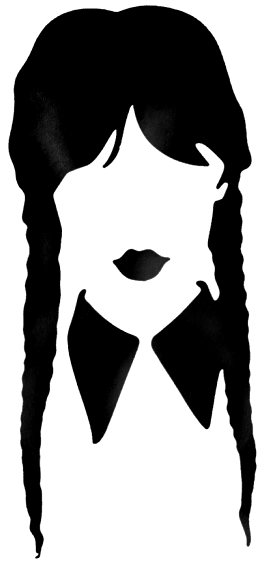
\includegraphics[height=1.35em]{figures/icons/mira-silhouette.png}}{}}}\enspace{\scshape\color{black}Scene}\enspace\textperiodcentered\enspace{\bfseries #1}\pdblockheadingend{\itshape #2}}%
    \end{tcolorbox}\par\addvspace{8pt plus 2pt}%
  }%
  \long\def\xrefbox#1{\par\pd@settle\addvspace{4pt}\noindent\pd@marginhead{See also}{\small #1}\par\addvspace{4pt}}%
  % A generic "Thesis" margin label does not identify which claim matters.
  % Keep the prose; use an authored keyidea head only when it adds meaning.
  \long\def\pdthesis#1{\par\pd@settle\addvspace{6pt plus 1pt}\noindent#1\par\addvspace{6pt plus 1pt}}%
  \long\def\pullquote#1{\pdthesis{#1}}%
}
\makeatother

% Shared visual language for the Book's figures -- version 2.
% Twin: book/figures/pd-figure-language.tex (byte-identical; edit both).
% The standard behind it, the migration from v1 and the QA loop live in
% skills/tikz-diagram-craft/ (SKILL.md, references/figure-standard.md).
%
% This file defines voices, hues, weights and marks -- not layouts.  Every
% figure still chooses a grammar from its reader question.
%
% ===========================================================================
% 1.  THE TYPE LADDER.  Three voices, one size, each tied to a role.
%       pd title   bold      panel titles, row and actor heads, column heads
%       pd label   upright   node text, state names, axis titles, tick words,
%                            relation words on an edge, badge numerals
%       pd note    italic    the one annotation a figure is allowed
%     `pd tag` is the label voice knocked out of the page, for a word that
%     must sit near a rule.  `pd kind` (small caps) is a one- or two-word kind
%     tag, never a title.  Every piece of figure text is mixed case; \texttt
%     only for identifiers that are literally code; math mode for symbols.
%
% 2.  THE COLOUR SYSTEM.  Hue is meaning, and the meanings cross chapters.
%     The figure's own subject is drawn in the CHAPTER hue (`pd focus ...`),
%     resolved from \pdcurrentchaptercolor, which the Book sets per chapter;
%     a fragment declares its standalone fallback with \pdfigurehue{...}.
%     Anything else the figure names takes its concept hue:
%       pd truth       pdcobalt   kernel, truth, the thing being specified
%       pd legible     pdteal     legibility, digest, inspection
%       pd ready       pdhealth   ready, coordinated, admitted, passing
%       pd protocol    pdindigo   protocol, federation, the wire
%       pd identity    pdviolet   identity, continuity, a card, an ID
%       pd reputation  pdrust     reputation, trust earned over time
%       pd value       pdgold     economy, value, settlement, payment
%       pd breach      pderror    breach, refusal, revocation, correction
%       pd warn        pdamber    warning; rules and stripes only, never text
%     Each concept X yields X, X rule, X arrow, X state, X fill, X datum and
%     X label.  Two to four hues a figure; colour is always doubled by shape,
%     dash, weight or a word (breach and warn are dashed as well as coloured).
%
% 3.  THE WEIGHT LADDER.  Exactly three weights, .5 / .9 / 1.6 pt
%     (1 : 1.8 : 3.2).  .5: hairline, guide, tick, artifact edge, fill edge,
%     mark outline, badge.  .9: rule, arrow, state edge, concept arrow.
%     1.6: spine, focus rule, focus and concept state edges, concept rule.
%     A reader sees which line is the subject.  Tips scale with the stroke.
%
% 4.  THE SURFACE LADDER.  pd state (page ground, ink edge) < pd artifact
%     (page ground, grey edge, subordinate) < pd focus state and the concept
%     states (24 % tint, edged in the same hue).  Text is always ink.  A
%     terminal state has a double boundary; an automaton's states are circles
%     (`pd automaton state/focus/terminal`); a ledger's pools are buckets
%     joined by pipes (`pd bucket`, `pd pipe`); a trust boundary is a dashed
%     rectangle (`pd trust boundary`).
%
% 5.  THE GROUND.  Body pages print on white, so every knockout and every
%     neutral surface is `pdpage` (white), never cream: a cream backing on a
%     white page reads as a sticker, which is what v1's figures were covered
%     in.  Neutral regions (Gantt bands, wells) are a warm grey tint.
%
% 6.  EDITIONS.  The Book sets \pdedition (maritime | swiss | technical) and
%     figures/pd-figure-language-<edition>.tex restyles the same names, so one
%     drawing renders in each edition's character.  A fragment that names a
%     raw colour (hhteal, pdcobalt!40, blue) bypasses this; name a role.
% ===========================================================================
% Libraries every v2 mark needs (diamonds, braces, markings), and
% pgfplots for computed plots. This file is \input in every preamble (the
% Book's and each standalone chapter's), so a plot works in all of them.
\usetikzlibrary{arrows.meta,matrix,patterns.meta,positioning,calc,fit,
  backgrounds,shapes.geometric,shapes.multipart,shapes.misc,decorations.pathreplacing,
  decorations.markings,quotes,intersections}
\RequirePackage{pgfplots}
\pgfplotsset{compat=1.18}
\usepgfplotslibrary{fillbetween,groupplots}

\colorlet{pdpage}{white}

% --- the chapter hue, resolved late --------------------------------------
% \pdfigurehue{pdindigo} on the line before a tikzpicture names the hue the
% figure is drawn in when it is compiled outside the Book (a standalone
% chapter, or the skill's renderer).  Inside the Book the preamble has already
% defined \pdcurrentchaptercolor and the chapter opener sets it, so there the
% opener wins and \providecommand does nothing.  Local to the figure's group.
\newcommand{\pdfigfraghue}{pdcobalt}
\newcommand{\pdfigurehue}[1]{%
  \renewcommand{\pdfigfraghue}{#1}%
  \providecommand{\pdcurrentchaptercolor}{#1}}
\newcommand{\pdsetfocushue}{%
  \ifdefined\pdcurrentchaptercolor
    \colorlet{pdfocus}{\pdcurrentchaptercolor}%
  \else
    \colorlet{pdfocus}{\pdfigfraghue}%
  \fi}
\colorlet{pdfocus}{pdcobalt}

% ===========================================================================
% THE TYPOGRAPHIC LAW
% ===========================================================================
% Companion to the line-weight law in figures/pd-palette.tex (1px texture,
% 1.5px linework, 2px enclosure). Same shape of rule: name the roles, fix the
% values, one place.
%
% ONE SIZE. Every named text role in a figure is \pdfiglabelsize
% (= \footnotesize). Roles separate by WEIGHT, SLOPE, FAMILY and INK -- never
% by size. A fragment never writes a size command of its own; if a distinction
% needs making, it takes the role that makes it.
%
% Where the size comes from. Measured, not chosen:
%   \tiny  \scriptsize  \footnotesize  \small  \normalsize
%   5.23    6.97          8.72           9.55    10.46  pt   Book (10.5pt
%                                                            Pagella, 4.5in
%                                                            column, 7x10in)
%   5.98    7.97          8.97           9.96    10.91  pt   standalone chapter
%                                                            (11pt Latin Modern)
% \scriptsize renders at 6.97pt in the Book -- under figcheck's 7pt T1 floor
% before a single width promotion, so it is illegal by measurement, not taste.
% \footnotesize holds 8.72pt and still clears the floor at the 0.85 \resizebox
% limit craft-rules sets (7.41pt). It is also what the corpus already voted
% for: 78 of the 91 local font= declarations this law replaces were already
% \footnotesize, \footnotesize\bfseries or \footnotesize\itshape.
%
% \pdfigbasesize (= \small) is the tikzpicture's ambient size only, so an
% unstyled node is never SMALLER than a styled one; every named role steps
% down exactly one notch from it and none steps down twice.
%
% ONE FACE, AND IT IS THE DOCUMENT'S. \pdfiglabelfamily is empty by default,
% which means figure type inherits whatever face the document is setting --
% Palatino in the Book, Computer Modern in a standalone chapter. Figures
% agreeing with EACH OTHER is not the goal; figures agreeing with the
% paragraph beside them is. A fragment therefore never names a family. Not
% \sffamily (which resolves to Latin Modern Sans against a Computer Modern
% page and reads as a foreign object on it), not \rmfamily, not
% \fontfamily{...}. P18 in tikz_precheck.py is an error for exactly that.
% An edition MAY substitute a face -- the Swiss and technical editions set
% \pdfiglabelfamily to \pdgrotesk, because grotesk display is their declared
% character -- and it does so in ONE command in ONE file, so the substitution
% is a decision on the record rather than an accident in a fragment. The
% only family a fragment may ask for is the identifier one, and it asks for
% it by role (pd mono label / \pdfiglabelmono), never by \ttfamily.
%
% What the roles are, and what each one is for:
%   pd panel title        bold        the name of a panel
%   pd row label          bold        an actor/row name east of its lane
%   pd reverse row label  bold, cream a row name sitting on a dark band
%   pd axis label         regular     an axis title or a tick numeral
%   pd direct label       regular     a value or name riding its own mark
%   pd reverse label      regular, cream  a direct label on a dark band
%   pd mono label         mono        an identifier, path, or literal
%   pd verdict            bold        a terminal outcome stamp (CLEAR, REJECT)
%   pd note               italic      one aside per figure
%   pd legend             regular     a pgfplots legend entry
%   pd state / terminal / actor / artifact / decision   node text
%   pd axis               the whole pgfplots typographic block, one key
%   \pdfigsub             a gloss line under a heading INSIDE a node
%   \pdfigmath            math carrying a sub/superscript, inside a label
%
% A fragment that needs a compound style of its own composes it from a role
% above (`gate/.style={pd decision,minimum width=2cm}`), or, where no role
% fits, from the \pdfiglabel* handles here. It never writes a raw size
% command: P16 in skills/harbor-chartwork/scripts/tikz_precheck.py is an
% error for exactly that, and P10/P11 have been errors for \tiny and
% \scriptsize since before this law.
%
% What does NOT transfer from the screen rules these roles otherwise follow.
% The dataviz method those rules come from assumes an interactive chart: a
% tooltip carries any value a label could not fit, a filter row rescopes the
% view, hover lifts the hovered mark. A printed page has none of that, and the
% absence is not a defect to design around. The INTENT of the tooltip rule --
% "every value is reachable without gating" -- does transfer, and on this page
% it is discharged somewhere else: the value is in the caption, in the margin
% apparatus, or in the chapter's own worked example. So a label that will not
% fit inside its mark moves outside the mark or is dropped to the caption; it
% is never shrunk to fit, because there is no size below \footnotesize to shrink
% to, and never clipped. Do not add a hover affordance, a legend toggle, or a
% filter to a figure in this book.
%
% IDENTIFIERS GET ONE SPELLING. A key, a cell id, a file name or any other
% literal a reader could type is set in `pd mono label` (or \pdfiglabelmono
% inside a compound style), spelled exactly as the code spells it: sk_A, not
% skA and not sk with a subscript A; card0, not card-nought and not a Unicode
% subscript zero. A figure that shows the same identifier two ways has told
% the reader they are two things. The subscripted form belongs to MATHEMATICS
% ($\kappa_7$, an index into a sequence) and the literal form to CODE -- one
% figure may use both, for different objects, but never both for the same
% one. (A precheck for two spellings of one identifier inside a fragment is
% being added on another branch; this is the convention it will enforce.)
%
% SHAPE IS A CHANNEL, AND IT HAS TO SURVIVE THE PRINT SIZE. pd datum, pd
% focus datum and pd caution datum carry three different forms, because the
% house palette is three low-chroma print inks and every distinction it makes
% has to be doubled by something that is not colour. That only counts if the
% form is still legible at 2.1-2.7 pt: an edition that flattens all three to
% one form has removed the second channel and left the figure separating its
% classes by hue alone, which fails in greyscale and for a colour-blind
% reader. Any edition override that restyles a datum must keep three
% distinguishable forms, and must be checked on a render at 1.0x, not
% reasoned about from the point sizes.
%
% One screen rule that does NOT bind here, and why. "Text never wears the data
% colour" exists because a light categorical hue is illegible as text on a
% light surface. The house figure hues are print inks, not screen hues --
% hhink #1B1712, hhteal #00564C, hhamber #6B4500 -- and all three clear text
% contrast on cream, so a label MAY wear its series' ink to bind itself to a
% curve, which is direct labelling and saves a legend. The rule that survives
% is the reason behind it: text wears one of those three inks at full
% strength, or hhink!80!hhgray for recessive furniture, and nothing else. A
% tint of an ink (text=hhgray, text=hhteal!60) is not a role; it is a fade.
% ===========================================================================

\providecommand{\pdfiglabelfamily}{}            % an edition may set \pdgrotesk
\providecommand{\pdfiglabelsize}{\footnotesize} % every named text role
\providecommand{\pdfigbasesize}{\small}         % the picture's ambient size
\providecommand{\pdfiglabel}{\pdfiglabelfamily\pdfiglabelsize}
\providecommand{\pdfiglabelbold}{\pdfiglabel\bfseries}
\providecommand{\pdfiglabelitalic}{\pdfiglabel\itshape}
\providecommand{\pdfiglabelmono}{\pdfiglabelsize\ttfamily}
% The one role that is not a node style, because it lives INSIDE a node's text:
% the second line under a heading that glosses it ("reviewer role / obligation +
% capability + authority"). Every fragment that needed it reached for \tiny or
% \scriptsize, which is how seven \tiny and twelve \scriptsize survived P10/P11
% as hard errors in the corpus. It steps down by SLOPE and WEIGHT, not size, so
% it stays legible and stays legal, and it touches neither family nor ink --
% which is what lets it sit on a reversed node without vanishing.
\providecommand{\pdfigsub}{\mdseries\itshape}
% The one place the law's own size is not the right size.
%
% Measured, both preambles, on a subscripted label inside `pd direct label`:
%
%              base glyph   subscript   subscript as % of base
%   chapter      8.97pt       5.98pt            66.7%
%   Book         8.72pt       6.36pt            72.9%
%   promoted    10.91/10.46   7.97/7.64
%
% An earlier version of this comment said those subscripts are "under figcheck's
% 7pt T1 floor". They are not, and the correction is worth more than the claim
% was. T1 has TWO bands: running text is held to 7.0pt, and a span of three
% glyphs or fewer -- a sub/superscript, a tick numeral -- is held to 5.9pt
% (T1_SHORT_SPAN_PT). That second band is not a loophole. A subscript is set at
% roughly 70% of its base by every typesetter that has ever existed; holding one
% to the running-text floor would mean either no subscripts in figures at all,
% or a figure whose base type is 10pt against 8.72pt body text.
%
% So \pdfigmath is NOT a T1 remedy, and using it as one is how a rule gets
% applied where it does not belong. It exists because 5.98pt clears the
% short-span band by 0.08pt, and 0.08pt is not a margin: a font substitution, an
% edition that nudges \pdfigbasesize, or a chapter that loads a different math
% font puts that subscript under the band with nobody having decided anything.
% Promotion puts it at 7.97/7.64pt -- over even the running-text floor -- while
% the base glyph stays close enough to its neighbours that the label still reads
% as one label.
%
% Use it ONLY for a math group that carries a sub- or superscript. Plain math
% takes the label's own size like any other text, and P22 in tikz_precheck.py is
% an error if it does not.
\providecommand{\pdfigmath}{\normalsize}

% ---------------------------------------------------------------------------
% THE GUIDE DASH, IN ABSOLUTE POINTS, IN ONE PLACE.
%
% `pd guide` used to read `line width=.45pt,densely dotted`. `densely dotted`
% expands to `dash pattern=on \pgflinewidth off 1pt`, and \pgflinewidth is read
% when the KEY is processed, not when the path is stroked. So the Swiss
% edition's `pd guide/.append style={draw=hhink!40,line width=.5pt}` widened the
% stroke and left the dash at the .45pt already baked into it. The canonical
% Book therefore shipped a 0.448pt dot on a 0.498pt stroke.
%
% MEASURED IN THE SHIPPED ARTIFACT, not in a probe: 50 guide strokes sampled
% pixel by pixel in the committed coordination-papers-mega-volume.pdf, at 150
% dpi / 1.0x.
%
%   on 0.448pt = 0.93 device px -- UNDER ONE PIXEL; off 0.996pt = 2.08 px
%   the dash DECLARES 69% of each line's length as gap
%   only 34% of each line's pixels actually reach paper
%   35.4% of three-period windows contain NO pixel that reaches paper at all
%
% That last number is the defect. The gap (2.08 px) is narrower than the
% antialias spread of a 0.93 px stroke, so as the pattern's phase drifts along a
% line the gaps fill in: over a third of every guide's length there is no gap
% left and it is a continuous grey stroke, while the rest of the same line still
% reads as dots. The ink arrives. The DOTTEDNESS does not. A reader sees one
% line that is dotted here and solid there, and no author chose that.
%
% Twenty-five of the corpus's thirty-six guide draws use dottedness to mean
% "this line is not a drawn edge", so twenty-five of them were making a
% distinction the page does not carry.
%
% After, same measurement, same probe geometry, Book preamble:
%   on 1.2pt = 2.50 px, off 2.0pt = 4.17 px, stroke .7pt = 1.45 px
%   0.0% of three-period windows are without paper -- every gap survives,
%     at every phase
%   50% of pixels reach paper against 62.5% declared, the shortfall now being
%     the stroke's antialias skirt rather than the whole signal
%
% ON THE INK, because the obvious reading of this change is wrong. The BASE pair
% was never the problem: hhgray!62 against the hairline's hhgray!78 is 0.411
% against 0.517 of nominal ink, well apart. The problem is that the Book renders
% the SWISS edition (\pdedition defaults to swiss; the committed Book PDF is
% full of hhink!40 guides), where the pair was hhink!40 against hhink!45 -- 4.6%
% of the grey scale. Deleting the Swiss override, which is the right fix for the
% geometry, makes the base ink govern the Book too -- and hhgray!62 is 0.411
% against the Book hairline's 0.410. The same grey, to a thousandth. So the base
% ink has to move, or the dash would go back to carrying the whole distinction
% by itself, which is how this started.
%
% hhink!70 measured against the hairline, mean ink on the page at 150 dpi:
%   chapter  guide 0.0502  hairline 0.0790   guide is 64% of the hairline
%   Book     guide 0.0545  hairline 0.0671   guide is 81% of the hairline
% Per DOT it is 0.638 against 0.410 -- unmistakably a different mark. In MEAN it
% is still lighter than the hairline -- so it still recedes. Two channels, both
% working, instead of one that does not.
%
% The replacement is stated absolutely and measures phase-STABLE: every dot
% renders at the same weight wherever it falls on the grid (peak column ink
% 0.808, invariant across twelve sub-pixel offsets). It is a macro rather than
% three numbers because an edition that restates one of them and not the others
% is how this defect happened. The geometry is a LEGIBILITY FLOOR, not an
% edition's character: an edition may move the guide's ink, and states the
% geometry through these two macros so it cannot half-restate it.
%
% Any dash in this corpus is stated in absolute points. The `dotted` family
% (`dotted`, `densely dotted`, `loosely dotted`) derives its on-length from the
% line width and is therefore banned -- P23 in tikz_precheck.py. `dashed` and
% its relatives are absolute (on 3pt off 3pt) and are fine.
\providecommand{\pdguidewidth}{.7pt}
% Three lengths, not one macro holding the whole key: pgfkeys splits a key list
% on `,` and `=` before expanding anything (so a macro carrying `dash
% pattern=...` is read as one key NAME), and TikZ's dash-pattern scanner reads
% the literal words `on`/`off` without expanding a macro that hides them. A
% dimension after each word does expand, which is the seam that works.
\providecommand{\pdguideon}{1.2pt}
\providecommand{\pdguideoff}{2.0pt}

\tikzset{
  % --- picture level: one size, one default tip, the chapter hue -----------
  % A figure label is a name, not prose: it never hyphenates.
  pd figure/.style={font=\pdfiglabelfamily\pdfigbasesize,text=pdink,line cap=round,line join=round,
    >={Stealth[length=2.6pt 3.2,width=2.0pt 2.4]},/utils/exec=\pdsetfocushue,
    every node/.append style={execute at begin node={%
      \hyphenpenalty=10000\exhyphenpenalty=10000\relax}}},
%
  % --- 1. the voices ---------------------------------------------------------
  pd title/.style={font=\pdfiglabelbold,text=pdink,align=center},
  pd label/.style={font=\pdfiglabel,text=pdink,align=center},
  pd note/.style={font=\pdfiglabelitalic,text=pdinkmuted,align=left},
  pd kind/.style={font=\pdfiglabel\scshape,text=pdinkmuted,align=center},
  pd tag/.style={pd label,fill=pdpage,inner sep=1.7pt},
%
  % --- 4. surfaces -----------------------------------------------------------
  pd state/.style={pd label,draw=pdink,line width=.9pt,fill=pdpage,
    rounded corners=1pt,inner xsep=6pt,inner ysep=4.5pt,minimum height=7.4mm},
  % a terminal state carries a double boundary, as every automaton text draws it
  pd terminal/.style={pd state,double=pdpage,double distance=1.1pt,line width=.5pt},
  pd artifact/.style={pd label,draw=pdinkmuted!60,line width=.5pt,fill=pdpage,
    rounded corners=1pt,inner xsep=5pt,inner ysep=3.5pt,minimum height=6.2mm},
  pd panel/.style={draw=pdinkmuted!55,line width=.5pt,
    dash pattern=on 2.4pt off 2pt,rounded corners=2.5pt,inner sep=7pt,align=center},
  pd hatch/.style={pattern={Lines[angle=45,distance=4pt,line width=.3pt]},
    pattern color=pdinkmuted!70},
  pd neutral fill/.style={fill=pdinkmuted!12,draw=pdinkmuted!55,line width=.5pt},
%
  % --- 3. strokes ------------------------------------------------------------
  pd hairline/.style={draw=pdinkmuted!45,line width=.5pt},
  % Absolute dash, from the typographic law's three macros above: a guide is a
  % definite dotted construction line, darker per dot than the hairline and
  % lighter in mean ink. A lattice is the quiet continuous grid a figure stands on.
  pd guide/.style={draw=pdink!70,line width=\pdguidewidth,dash pattern=on \pdguideon off \pdguideoff},
  pd lattice/.style={draw=pdinkmuted!40,line width=.4pt},
  pd tick/.style={draw=pdinkmuted!75,line width=.5pt},
  pd rule/.style={draw=pdink,line width=.9pt},
  pd spine/.style={draw=pdink,line width=1.6pt},
  pd thin arrow/.style={draw=pdinkmuted!75,line width=.5pt,->},
  pd arrow/.style={pd rule,->},
  pd spine arrow/.style={pd spine,->},
%
  % --- the chapter hue, as the figure's focus --------------------------------
  pd focus rule/.style={draw=pdfocus,line width=1.6pt},
  pd focus arrow/.style={pd focus rule,->},
  pd focus state/.style={pd state,draw=pdfocus,line width=1.6pt,fill=pdfocus!24},
  % The single solid chapter-colour surface in a figure: use only for the
  % culmination or object the reader should name after five seconds. Editions
  % may render ordinary focus with a pale field while keeping this one solid.
  pd climax state/.style={pd focus state},
  % a member of the subject's set when the set, not one node, is the subject:
  % edged in the chapter hue, never filled, so the one solid node stays unique
  pd focus outline/.style={pd state,draw=pdfocus,line width=1.2pt,fill=pdpage},
  pd focus fill/.style={fill=pdfocus!24,draw=pdfocus,line width=.5pt},
  pd focus datum/.style={circle,fill=pdfocus,draw=pdpage,line width=.5pt,inner sep=2.6pt},
  pd focus label/.style={pd label,text=pdfocus!85!pdink},
%
  % --- marks -----------------------------------------------------------------
  pd datum/.style={circle,fill=pdink,draw=pdpage,line width=.5pt,inner sep=2.3pt},
  pd badge/.style={pd label,circle,draw=pdink,line width=.5pt,fill=pdpage,
    inner sep=.5pt,minimum size=5.0mm},
  pd focus badge/.style={pd badge,draw=pdfocus,line width=.9pt,fill=pdfocus!24},
  % --- conventions shared by every chapter (Critical Analysis, 2026-09-08) ---
  % Automata: states are circles, terminal (accepting) states double circles;
  % edge words are short action names; guards go in an aligned legend table.
  pd automaton state/.style={pd label,circle,draw=pdink,line width=.9pt,fill=pdpage,
    minimum size=11mm,inner sep=1pt},
  pd automaton focus/.style={pd automaton state,draw=pdfocus,line width=1.6pt,fill=pdfocus!24},
  pd automaton terminal/.style={pd automaton state,double=pdpage,double distance=1.1pt,
    line width=.5pt},
  pd initial/.style={draw=pdink,line width=.9pt,->},
  % Ledgers: asset pools are rectangular buckets (open at the top) joined by
  % directed pipes; the conserved sum is set as an equation under the rails.
  pd bucket/.style={pd label,draw=none,minimum width=2.2cm,minimum height=1.3cm,
    append after command={\pgfextra{\draw[draw=pdink,line width=.9pt]
      (\tikzlastnode.north west) -- (\tikzlastnode.south west)
      -- (\tikzlastnode.south east) -- (\tikzlastnode.north east);}}},
  pd pipe/.style={draw=pdink,line width=.9pt,double=pdpage,double distance=2.2pt,
    -{Stealth[length=3.4pt 2,width=5.2pt]}},
  pd focus pipe/.style={pd pipe,draw=pdfocus},
  % Trust boundaries: a dashed rectangle is the Dolev-Yao interface; a vector
  % that escapes it is drawn in pd breach and named.
  pd trust boundary/.style={draw=pdink,line width=.9pt,dash pattern=on 4pt off 2.4pt,
    rounded corners=0pt,inner sep=8pt},
  % a stroke that ends at a badge is shortened, so no rule touches the numeral
  pd to badge/.style={shorten >=2pt},
  pd from badge/.style={shorten <=2pt},
}

% ===========================================================================
% 7.  PLOTS.  A plot is computed by a committed script, never sketched.  `pd
%     axis` is the one axis grammar: two spines (left, bottom), ticks out, no
%     box, no grid unless asked (`pd grid`), tick words in the label voice,
%     numbers with a thin-space thousands separator, room outside the plot for
%     direct labels (clip=false).  Series are named at their ends, not in a
%     legend: `pd series` (ink), `pd focus series` (chapter hue), and
%     `pd X series` for a concept; breach and warn series are dashed.  A
%     region between curves is `pd focus fill`/`X fill` with fillbetween.
%     Width: `width=` is the plot box (scale only axis); leave about 1.6 cm
%     of the 11.4 cm column for the y tick words and title.
% ===========================================================================
\pgfplotsset{
  pd axis/.style={
    scale only axis,width=8.8cm,height=4.6cm,
    axis lines*=left,axis line style={draw=pdink,line width=.5pt,-},
    tick align=outside,major tick length=3pt,minor tick length=0pt,
    tick style={draw=pdink,line width=.5pt},
    tick label style={pd label,text=pdinkmuted},
    label style={pd label},title style={pd title},
    every axis title/.append style={yshift=-2pt},
    enlargelimits=false,clip=false,
    grid=none,
    legend style={draw=none,fill=none,font=\pdfiglabel},
    /pgf/number format/1000 sep={\,},
    every axis plot/.append style={line width=.9pt,line join=round,mark size=1.7pt},
  },
  pd grid/.style={ymajorgrids,major grid style={draw=pdinkmuted!30,line width=.4pt}},
  pd series/.style={draw=pdink,mark=*,mark options={fill=pdink,draw=pdpage,line width=.5pt,solid}},
  pd focus series/.style={draw=pdfocus,line width=1.6pt,mark=*,
    mark options={fill=pdfocus,draw=pdpage,line width=.5pt,solid}},
  pd muted series/.style={draw=pdinkmuted!70,line width=.9pt,mark=none},
}
\newcommand{\pdplotconcept}[2]{%
  \pgfplotsset{#1 series/.style={draw=#2,mark=*,
    mark options={fill=#2,draw=pdpage,line width=.5pt,solid}}}}
\pdplotconcept{pd truth}{pdcobalt}
\pdplotconcept{pd legible}{pdteal}
\pdplotconcept{pd ready}{pdhealth}
\pdplotconcept{pd protocol}{pdindigo}
\pdplotconcept{pd identity}{pdviolet}
\pdplotconcept{pd reputation}{pdrust}
\pdplotconcept{pd value}{pdgold}
\pgfplotsset{
  pd breach series/.style={draw=pderror,dash pattern=on 3.2pt off 2.2pt,mark=diamond*,
    mark options={fill=pderror,draw=pdpage,line width=.5pt,solid}},
  pd warn series/.style={draw=pdamber,dash pattern=on 3.2pt off 2.2pt,mark=none},
}

% ===========================================================================
% Supplied visual-guide primitives: native Book type, deliberate strokes,
% readable Stealth heads, open markers, and a quiet quantitative grid.
% These are opt-in: old diagrams need spacing review before thicker arrows.
\tikzset{
  pd guide step/.style={pd artifact,draw=pdink,fill=pdpage,line width=1pt,
    align=center,minimum height=40pt,inner xsep=5pt,inner ysep=6pt},
  pd guide arrow/.style={draw=pdcobalt,line width=1.15pt,
    -{Stealth[length=7pt,width=4.4pt]},shorten <=2pt,shorten >=2pt},
}
\newcommand{\pdflowstep}[4]{%
  \node[pd guide step,text width=#4] (#1) at #2 {#3};}
\newcommand{\pdflowlink}[2]{%
  \draw[pd guide arrow] (#1.east)--(#2.west);}
\pgfplotsset{
  pd evidence axis/.style={pd axis,
    axis line style={draw=pdink,line width=1pt,-},
    tick style={draw=pdink,line width=.8pt},
    grid=major,major grid style={draw=pdinkmuted!20,line width=.35pt},
    axis background/.style={fill=pdpage}},
  pd evidence measured/.style={draw=pdcobalt,line width=1.35pt,mark=*,
    mark size=2.6pt,mark options={fill=pdpage,draw=pdcobalt,line width=1.1pt}},
  pd evidence comparison/.style={draw=pdink,line width=1.1pt,
    dash pattern=on 4pt off 2.5pt,mark=square*,mark size=2.2pt,
    mark options={fill=pdink,draw=pdink,solid}},
}
% Analytic curves, not sampled observations. Integer samples preserve the
% meaning of reviewer count; callers set axes and name their assumptions.
\newcommand{\pdindependentmisses}[2]{%
  \addplot[pd evidence measured,domain=1:#2,samples=#2] {100*(1-#1)^x};}
\newcommand{\pdreviewcost}[1]{%
  \addplot[pd evidence measured,domain=1:#1,samples=#1] {x};}
% 8.  UML.  The Book's engineering diagrams use UML 2.5 notation, so a reader
%     who knows UML reads them without a key.  Four kinds:
%     STATE MACHINE  `pd uml state` (rounded), `pd uml focus state`, a
%       composite drawn with `pd uml composite` around its substates plus a
%       compartment of internal transitions; `pd uml initial` (filled dot),
%       `pd uml final` (bullseye), `pd uml choice` (diamond); transitions are
%       `pd uml transition` (open arrowhead) labelled  event [guard] / effect.
%     SEQUENCE  `pd uml head` (lifeline head), `pd uml lifeline` (dashed),
%       `pd uml activation` (thin bar), messages `pd uml sync` (filled head),
%       `pd uml async` (open head), `pd uml reply` (dashed, open head),
%       `pd uml fragment` + `pd uml fragment tag` for alt / opt / loop.
%     COMPONENT  `pd uml component` with \pdumlicon{node} (the component
%       glyph) and a <<component>> keyword; `pd uml port`; provided interface
%       \pdumlprovided{from}{to}{name} (lollipop), required \pdumlrequired (socket).
%     ERD (crow's foot)  `pd er entity` (rectangle split: name, then rows;
%       mark keys PK / FK in the row text), relationship lines `pd er rel`
%       with tips `er one`, `er many`, `er zero or one`, `er one or many`,
%       `er zero or many` at either end.
% ===========================================================================
\pgfdeclarearrow{
  name = pd crow,
  parameters = {\the\pgfarrowlength,\the\pgfarrowwidth},
  setup code = {%
    \pgfarrowssettipend{0pt}%
    \pgfarrowssetlineend{0pt}%
    \pgfarrowssetbackend{-\pgfarrowlength}%
    \pgfarrowsupperhullpoint{0pt}{.5\pgfarrowwidth}%
    \pgfarrowsupperhullpoint{-\pgfarrowlength}{0pt}%
    \pgfarrowssavethe\pgfarrowlength
    \pgfarrowssavethe\pgfarrowwidth},
  drawing code = {%
    \pgfsetdash{}{0pt}%
    \pgfpathmoveto{\pgfqpoint{-\pgfarrowlength}{0pt}}%
    \pgfpathlineto{\pgfqpoint{0pt}{.5\pgfarrowwidth}}%
    \pgfpathmoveto{\pgfqpoint{-\pgfarrowlength}{0pt}}%
    \pgfpathlineto{\pgfqpoint{0pt}{-.5\pgfarrowwidth}}%
    \pgfusepathqstroke},
  defaults = {length=2.4mm, width=3.0mm}
}
\tikzset{
  % state machine
  pd uml state/.style={pd state,rounded corners=4.5pt},
  pd uml focus state/.style={pd focus state,rounded corners=4.5pt},
  pd uml terminal/.style={pd terminal,rounded corners=4.5pt},
  pd uml composite/.style={draw=pdink,line width=.9pt,rounded corners=7pt,fill=none,inner sep=0pt},
  pd uml initial/.style={circle,fill=pdink,draw=none,minimum size=2.4mm,inner sep=0pt},
  pd uml final/.style={circle,draw=pdink,line width=.9pt,fill=pdpage,minimum size=3.6mm,inner sep=0pt,
    path picture={\fill[pdink] (path picture bounding box.center) circle (1.1mm);}},
  pd uml choice/.style={diamond,draw=pdink,line width=.9pt,fill=pdpage,minimum size=4.2mm,inner sep=0pt},
  pd uml transition/.style={pd rule,-{Straight Barb[length=2.2pt 2.2,width=4.4pt 2.2]}},
  pd uml focus transition/.style={pd focus rule,-{Straight Barb[length=2.2pt 2.2,width=4.4pt 2.2]}},
  pd uml breach transition/.style={pd rule,draw=pderror,dash pattern=on 3.2pt off 2.2pt,
    -{Straight Barb[length=2.2pt 2.2,width=4.4pt 2.2]}},
  % sequence
  pd uml head/.style={pd state,rounded corners=0pt,minimum height=6.8mm},
  pd uml lifeline/.style={draw=pdinkmuted!75,line width=.5pt,dash pattern=on 3pt off 2pt},
  pd uml activation/.style={draw=pdink,line width=.5pt,fill=pdpage,minimum width=2.2mm,inner sep=0pt},
  pd uml sync/.style={pd rule,-{Triangle[length=3.2pt 1.6,width=3.2pt 1.6]}},
  pd uml async/.style={pd rule,-{Straight Barb[length=2.4pt 2,width=4.4pt 2]}},
  pd uml reply/.style={pd rule,dash pattern=on 3pt off 2pt,-{Straight Barb[length=2.4pt 2,width=4.4pt 2]}},
  pd uml fragment/.style={draw=pdink,line width=.5pt,fill=none,inner sep=6pt},
  pd uml fragment tag/.style={pd label,font=\footnotesize\bfseries,draw=pdink,line width=.5pt,fill=pdpage,
    inner xsep=3pt,inner ysep=2pt,chamfered rectangle,chamfered rectangle corners=south east,
    chamfered rectangle xsep=2pt},
  % component
  pd uml component/.style={pd state,rounded corners=0pt,align=center,inner xsep=8pt,inner ysep=6pt,minimum height=11mm},
  pd uml port/.style={rectangle,draw=pdink,line width=.5pt,fill=pdpage,minimum size=2mm,inner sep=0pt},
  % ERD
  pd er entity/.style={pd label,rectangle split,rectangle split parts=2,rectangle split part align={center,left},
    draw=pdink,line width=.9pt,fill=pdpage,inner xsep=5pt,inner ysep=3pt,align=left,
    rectangle split part fill={pdinkmuted!12,pdpage}},
  pd er rel/.style={pd rule},
  er one/.tip={Bar[width=3.0mm,sep=1.2pt]Bar[width=3.0mm]},
  er many/.tip={Bar[width=3.0mm,sep=1.4pt]pd crow},
  er zero or one/.tip={Circle[open,length=1.8mm,width=1.8mm,sep=1.2pt,fill=pdpage]Bar[width=3.0mm]},
  er one or many/.tip={Bar[width=3.0mm,sep=1.4pt]pd crow},
  er zero or many/.tip={Circle[open,length=1.8mm,width=1.8mm,sep=1.2pt,fill=pdpage]pd crow},
}
% the component glyph, drawn in the top-right corner of a component node
\newcommand{\pdumlicon}[1]{%
  \begin{scope}[shift={($(#1.north east)+(-4.2mm,-2.6mm)$)},x=1mm,y=1mm]
    \draw[pdink,line width=.5pt,fill=pdpage] (0,-1.1) rectangle (2.6,1.1);
    \draw[pdink,line width=.5pt,fill=pdpage] (-.6,.25) rectangle (.6,.65);
    \draw[pdink,line width=.5pt,fill=pdpage] (-.6,-.65) rectangle (.6,-.25);
  \end{scope}}
% a provided interface (lollipop) from a node side to a point, with its name
\newcommand{\pdumlprovided}[3]{%
  \draw[pd rule] (#1) -- (#2);
  \draw[pd rule,fill=pdpage] (#2) circle (1.3mm);
  \node[pd label,anchor=south] at ($(#2)+(0,1.6mm)$) {#3};}
% a required interface (socket): a half-circle open toward the provider
\newcommand{\pdumlrequired}[4]{% from, to, name, facing angle of the socket's opening
  \draw[pd rule] (#1) -- (#2);
  \draw[pd rule] ($(#2)+(#4+90:1.9mm)$) arc[start angle=#4+90,end angle=#4+270,radius=1.9mm];
  \node[pd label,anchor=north] at ($(#2)+(0,-2.4mm)$) {#3};}

% --- 2. the concept map, as styles, so a drawing never chooses a hue --------
% An edition file may \renewcommand\pdconcept before the map below expands.
\newcommand{\pdconcept}[2]{%
  \tikzset{%
    #1/.style={draw=#2,text=pdink},
    #1 rule/.style={draw=#2,line width=1.6pt},
    #1 arrow/.style={draw=#2,line width=.9pt,->},
    #1 state/.style={pd state,draw=#2,line width=1.6pt,fill=#2!24},
    #1 fill/.style={fill=#2!24,draw=#2,line width=.5pt},
    #1 datum/.style={circle,fill=#2,draw=pdpage,line width=.5pt,inner sep=2.6pt},
    #1 label/.style={pd label,text=#2!85!pdink},
  }}

% --- 6. the edition layer, loaded before the concept map expands ----------
\ifdefined\pdedition\IfFileExists{figures/pd-figure-language-\pdedition.tex}{\input{figures/pd-figure-language-\pdedition}}{}\fi

\pdconcept{pd truth}{pdcobalt}
\pdconcept{pd legible}{pdteal}
\pdconcept{pd ready}{pdhealth}
\pdconcept{pd protocol}{pdindigo}
\pdconcept{pd identity}{pdviolet}
\pdconcept{pd reputation}{pdrust}
\pdconcept{pd value}{pdgold}
\pdconcept{pd breach}{pderror}
\pdconcept{pd warn}{pdamber}
% Breach and warning read as refusals, so they are dashed as well as
% coloured, and a breach mark is a diamond where every other mark is a circle.
% Amber is never text (3.71:1 on white); a warn label is set in ink.
\tikzset{
  pd breach rule/.append style={dash pattern=on 3.2pt off 2.2pt},
  pd breach arrow/.append style={dash pattern=on 3.2pt off 2.2pt},
  pd warn rule/.append style={dash pattern=on 3.2pt off 2.2pt},
  pd warn arrow/.append style={dash pattern=on 3.2pt off 2.2pt},
  pd breach datum/.append style={diamond},
  pd warn label/.style={pd label},
}

% ===========================================================================
% v1 NAMES.  Kept so every existing fragment still compiles; they resolve to
% the v2 roles, so an untouched figure inherits the ladder.  New work uses the
% v2 names (skills/tikz-diagram-craft/references/migration-v1-to-v2.md).
% ===========================================================================
\tikzset{
  pd row label/.style={pd title,anchor=east},
  pd panel title/.style={pd title,align=left},
  pd axis label/.style={pd label},
  % Direct labels sit beside their mark; they do not erase a line or box
  % underneath themselves. A label that needs a paper knockout is misplaced
  % and must be moved, not given an invisible patch.
  pd direct label/.style={pd tag,fill=none,align=left},
  pd actor/.style={pd state},
  pd boundary/.style={pd panel},
  pd caution rule/.style={pd breach rule},
  pd caution arrow/.style={pd breach arrow},
  pd caution fill/.style={pd breach fill},
  pd caution datum/.style={pd breach datum},
}

% ===========================================================================
% Roles named on main by the typographic law (#10191), expressed on the v2
% roles so an edition's .append style on the parent reaches them. `pd danger`
% is main's name for what v2 calls `pd breach` (red, dashed, diamond marks);
% both names resolve to one family. Main's hairline-boxed fact badge is
% `pd fact badge`: v2's `pd badge` is the numbered guard/step marker.
% ===========================================================================
\tikzset{
  pd danger rule/.style={pd breach rule},
  pd danger arrow/.style={pd breach arrow},
  pd danger fill/.style={pd breach fill,text=pdink},
  pd danger datum/.style={pd breach datum},
  pd ink fill/.style={fill=pdink,draw=pdink,line width=.4pt,text=pdpage},
  pd decision/.style={pd state,diamond,aspect=1.55,font=\pdfiglabelbold,
    minimum height=0pt,inner xsep=3pt,inner ysep=3pt},
  pd mono label/.style={pd direct label,font=\pdfiglabelmono,inner xsep=2.5pt,inner ysep=2.5pt},
  pd verdict/.style={pd direct label,font=\pdfiglabelbold},
  pd reverse label/.style={pd direct label,text=pdpage,fill=none},
  pd reverse row label/.style={pd row label,text=pdpage},
  pd legend/.style={font=\pdfiglabel,text=pdink,draw=none,fill=none},
  pd kind tag/.style={pd kind,align=right},
  pd fact badge/.style={pd hairline,font=\pdfiglabel,text=pdink,align=center,
    inner sep=2.4pt,fill=none},
}

% Small reusable marks.  They deliberately avoid prose-bearing boxes.
\newcommand{\pdfigaxis}[4]{%
  \draw[pd rule,->] (#1,#2) -- (#3,#2);
  \node[pd label,anchor=west] at (#3,#2) {#4};
}
\newcommand{\pdfigvaxis}[4]{%
  \draw[pd rule,->] (#1,#2) -- (#1,#3);
  \node[pd label,anchor=south] at (#1,#3) {#4};
}

% Native-size, object-based evidence figures; shared by Book and chapters.
% Shared approved Swiss evidence drawing primitives. Keep both chapter roots identical.
\ifdefined\pdSwissEvidenceLoaded\else
\def\pdSwissEvidenceLoaded{1}
% Real ink-box gate; no declared coordinate envelope can substitute for this.
\newsavebox{\sgEvidenceBox}
\newcommand{\SGMeasuredFigure}[2]{%
  \sbox{\sgEvidenceBox}{#2}%
  \typeout{SG-GEOMETRY: #1,width=\the\wd\sgEvidenceBox,height=\the\dimexpr\ht\sgEvidenceBox+\dp\sgEvidenceBox\relax}%
  \ifdim\wd\sgEvidenceBox>325.215pt
    \PackageError{swiss-evidence}{Figure #1 exceeds the Book column}{Recompose at native text size; do not scale.}%
  \fi
  \usebox{\sgEvidenceBox}}
% Parent redraws after rejection of lab specimens 01,04,06.
% All coordinates are physical TeX points; no resizebox or transformed fonts.
\usetikzlibrary{arrows.meta,calc}
% Aliased onto the house palette (figures/pd-palette.tex), not \definecolor'd
% as independent HTML values: an edition that restyles pdcobalt/pdteal/...
% now restyles every SG figure with it. The six values were already
% bit-identical matches for pdcobalt/pdteal/pdviolet/pdamber/pderror/pdink;
% the alias turns that into a guarantee instead of a coincidence.
\colorlet{sgBlue}{pdcobalt}
\colorlet{sgTeal}{pdteal}
\colorlet{sgViolet}{pdviolet}
\colorlet{sgAmber}{pdamber}
\colorlet{sgRed}{pderror}
\colorlet{sgInk}{pdink}
\definecolor{sgGrid}{HTML}{D8C7A6}
% The one house size, inheriting the document's own face (the typographic
% law in pd-figure-language.tex): no \sffamily leak, no local \fontsize.
\newcommand{\SGType}{\pdfiglabel}
\tikzset{sg/base/.style={x=1pt,y=1pt,line cap=butt,line join=miter,
  every node/.style={font=\SGType,inner sep=0pt,text=sgInk}},
  sg/arrow/.style={-{Stealth[length=4.5pt,width=3.6pt]},draw=sgInk,line width=.85pt},
  sg/grid/.style={draw=sgGrid,line width=.3pt},
  sg/hash/.style={draw=sgBlue,fill=sgBlue!7,line width=1pt,minimum width=53pt,
    minimum height=27pt,inner sep=4pt,align=center},
  sg/sibling/.style={draw=sgAmber,fill=sgAmber!10,line width=1pt,minimum width=51pt,
    minimum height=27pt,inner sep=4pt,align=center},
  sg/check/.style={draw=sgInk,fill=white,line width=1pt,minimum width=92pt,
    minimum height=30pt,inner sep=5pt,align=center}}

% A folded record, not an undifferentiated rounded node. Width/height are pt.
\newcommand{\SGDocument}[6]{%
  \begin{scope}[shift={#2}]
    \path[draw=sgInk,fill=#5,line width=.85pt]
      (0,0)--({#3-7},0)--(#3,7)--(#3,#4)--(0,#4)--cycle;
    \draw[sgInk,line width=.65pt] ({#3-7},0)--({#3-7},7)--(#3,7);
    \node[minimum width=#3pt,minimum height=#4pt,text width=\dimexpr#3pt-12pt\relax,
      align=center] (#1) at ({#3/2},{#4/2}) {#6};
  \end{scope}}

\newcommand{\SGSurvival}{%
\begin{tikzpicture}[sg/base]
  % Three complete probability decades, percentages rather than tiny exponents.
  \foreach \x in {0,1,...,6}{\draw[sg/grid] ({35+30*\x},20)--({35+30*\x},140);}
  \foreach \y/\lab in {20/{0.1\%},60/{1\%},100/{10\%},140/{100\%}}{%
    \draw[sg/grid] (35,\y)--(215,\y);
    \draw[sgInk,line width=.65pt] (32,\y)--(35,\y);
    \node[anchor=east] at (28,\y) {\lab};}
  \draw[sgInk,line width=.85pt] (35,140)--(35,20)--(215,20);
  \foreach \x in {0,2,4,6}{%
    \draw[sgInk,line width=.65pt] ({35+30*\x},20)--({35+30*\x},17);
    \node[anchor=north] at ({35+30*\x},12) {$\x$};}
  \node[rotate=90] at (-9,80) {jobs still running (log scale)};
  \node[anchor=north] at (125,-5) {duration / mean duration};
  \draw[sgBlue,line width=1.5pt,domain=0:6,samples=100]
    plot ({35+30*\x},{140-120*ln(1+\x/2)/ln(10)});
  \draw[sgViolet,line width=1.2pt,dash pattern=on 4pt off 2.5pt,domain=0:6,samples=100]
    plot ({35+30*\x},{140-40*\x/ln(10)});
  % Endpoint leaders have allocated space; text does not lie on a curve.
  \draw[sgBlue,line width=.8pt] (215,67.75)--(224,67.75);
  \node[anchor=west,text=sgBlue,font=\SGType\bfseries] at (230,73) {Lomax};
  \node[anchor=west,text=sgBlue] at (230,60) {1.56\%};
  \draw[sgViolet,line width=.8pt,dashed] (215,35.77)--(224,35.77);
  \node[anchor=west,text=sgViolet,font=\SGType\bfseries] at (230,40) {exponential};
  \node[anchor=west,text=sgViolet] at (230,27) {0.248\%};
\end{tikzpicture}}

\newcommand{\SGTiming}{%
\begin{tikzpicture}[sg/base,y=-1pt]
  % This bracket spans COMMIT TO SYNC. It is not a range of hypothetical syncs.
  \path[draw=sgAmber!35,fill=sgAmber!9,line width=.5pt] (39,19) rectangle (253,49);
  \draw[sgAmber,line width=1pt] (39,18)--(39,9)--(253,9)--(253,18);
  \node[anchor=south,text=sgAmber,font=\SGType\bfseries] at (146,5) {?};
  \draw[sgInk,line width=.9pt] (39,27)--(39,45) (253,27)--(253,45);
  \draw[{Stealth[length=4.5pt,width=3.6pt]}-{Stealth[length=4.5pt,width=3.6pt]},
    sgAmber,line width=1.3pt] (40,36)--(252,36);
  \node[anchor=north,font=\SGType\bfseries] at (39,52) {commit};
  \node[anchor=north,font=\SGType\bfseries] at (253,52) {WAL sync};
  \node[anchor=west] at (0,86) {heartbeats received};
  \foreach \x/\label in {57/{s_1},117/{s_2},194/{s_3},278/{s_4}}{%
    \draw[sgViolet!70,dashed,line width=.55pt] (\x,104)--(\x,145);
    \node[anchor=south,text=sgViolet] at (\x,101) {$\label$};}
  \path[draw=sgAmber!35,fill=sgAmber!9,line width=.5pt] (158,108) rectangle (243,142);
  \draw[sg/grid] (0,139)--(306,139);
  \draw[sgTeal,line width=1.4pt]
    (0,132)--(25,132)--(25,116)--(33,116)--(33,132)
    --(85,132)--(85,116)--(93,116)--(93,132)
    --(145,132)--(145,116)--(153,116)--(153,132)--(306,132);
  \draw[sgRed,line width=1pt] (243,106)--(243,145);
  \node[anchor=north,text=sgRed] at (243,149) {deadline};
  \draw[sg/arrow] (0,174)--(306,174);
  \node[anchor=north east] at (306,179) {time};
\end{tikzpicture}}

\newcommand{\SGInclusion}{%
\begin{tikzpicture}[sg/base,y=-1pt]
  % Two independent inputs: a supplied proof and an issuer-authenticated root.
  \node[anchor=north west,font=\SGType\bfseries,text width=158pt,align=left] at (0,0)
    {Recompute from the receipt};
  \node[anchor=north west,font=\SGType\bfseries,text width=118pt,align=left] at (193,0)
    {Authenticate\\the checkpoint};
  \draw[sg/grid,step=15pt] (0,29) grid (175,194);
  \SGDocument{receipt}{(4,35)}{49}{34}{sgViolet!9}{receipt $P$}
  \node[sg/hash] (leaf) at (29,103) {$a=H_L(P)$};
  \node[sg/sibling] (sibone) at (108,103) {sibling $b$};
  \node[sg/hash] (inner) at (68,146) {$u=H_N(a,b)$};
  \node[sg/sibling] (sibtwo) at (146,146) {subtree $c$};
  \node[sg/hash,fill=sgBlue,text=white,minimum width=100pt] (computed) at (107,190)
    {$R'=H_N(u,c)$};
  \draw[sg/arrow,draw=sgViolet] (receipt.south)--(leaf.north);
  \draw[sg/arrow,draw=sgBlue] (leaf.south)--(inner.north west);
  \draw[sg/arrow,draw=sgAmber] (sibone.south)--(inner.north east);
  \draw[sg/arrow,draw=sgBlue] (inner.south)--(computed.north west);
  \draw[sg/arrow,draw=sgAmber] (sibtwo.south)--(computed.north east);
  \SGDocument{checkpoint}{(211,37)}{85}{48}{sgTeal!8}{signed root $R^*$\\size $n=4$\\signature $\sigma$}
  % The trusted key is an external input, not something the prover supplies.
  \draw[sgInk,line width=1pt] (218,113) circle (3.5pt);
  \draw[sgInk,line width=1pt] (221.5,113)--(233,113) (230,113)--(230,117) (233,113)--(233,117);
  \node[anchor=west] at (239,113) {trusted $pk_I$};
  \node[sg/check,minimum width=84pt] (verify) at (260,158) {verify $\sigma$\\result $A$};
  \draw[sg/arrow,draw=sgTeal] (checkpoint.east)--(311,61)--(311,158)--(verify.east);
  \draw[sg/arrow] (247,123)--(247,138)--(verify.north);
  \node[sg/check,minimum width=112pt,minimum height=34pt] (compare) at (164,245)
    {$A\ \land\ (R'=R^*)$};
  \draw[sg/arrow,draw=sgBlue] (computed.south)--(107,220)--(compare.north west);
  \draw[sg/arrow,draw=sgTeal] (verify.south)--(260,214)--(compare.north east);
  \node[anchor=east,text=sgTeal] at (250,204) {$R^*,A$};
  \node[draw=sgTeal,fill=sgTeal,text=white,minimum width=90pt,
    minimum height=27pt,font=\SGType\bfseries] (accept) at (76,299) {accept inclusion};
  \node[draw=sgRed,fill=white,text=sgRed,line width=1.2pt,minimum width=90pt,
    minimum height=27pt,font=\SGType\bfseries] (reject) at (256,299) {reject proof};
  \draw[sg/arrow,draw=sgTeal] (compare.south west)--(108,279)--(76,279)--(accept.north);
  \draw[sg/arrow,draw=sgRed] (compare.south east)--(220,279)--(256,279)--(reject.north);
  \node[anchor=south,text=sgTeal] at (82,275) {true};
  \node[anchor=south,text=sgRed] at (248,275) {false};
\end{tikzpicture}}

% Reusable geometry; load after swiss-redraws.tex. Real points, no scaling.
\newcommand{\SGDatabase}[4]{%
  \begin{scope}[shift={#2}]
    \path[draw=#3,fill=#3!7,line width=.9pt]
      (0,4)--(0,32) arc[start angle=180,end angle=360,x radius=24pt,y radius=5pt]
      --(48,4) arc[start angle=0,end angle=-180,x radius=24pt,y radius=5pt];
    \draw[draw=#3,fill=#3!7,line width=.9pt] (24,4) ellipse[x radius=24pt,y radius=5pt];
    \node[minimum width=48pt,minimum height=37pt,align=center] (#1) at (24,18) {#4};
  \end{scope}}

% Reader question: How do overlapping requests become ordered records?
% Evidence: schematic two-client history, not a runtime observation.
% Each request precedes commit 1; each reply follows its own committed record.
\newcommand{\SGWriterSequence}{%
\begin{tikzpicture}[sg/base,y=-1pt]
  % Recomposed at native size: a 22-character mono request label no longer
  % fits a 118pt lane gap at \pdfiglabelmono, so the HTTP verb is shortened
  % to the identifier it names and the resource it names ("auth.ts") moves
  % to the lane header, where it reads once instead of twice.
  \foreach \x/\lanelabel in {35/{{\pdfigmath$\alpha_{\text{auth}}$} (claude)},153/{Kernel (single writer)},275/{{\pdfigmath$\alpha_{\text{bill}}$} (codex)}}{
    \node[anchor=south,font=\pdfiglabelbold,align=center] at (\x,0) {\lanelabel};
    \draw[sg/grid] (\x,9)--(\x,237);}
  % Both invocations precede the first commit: overlapping client requests.
  \draw[sg/arrow,draw=sgViolet] (35,29)--(153,29);
  \node[anchor=south,text=sgViolet,font=\pdfiglabelmono] at (94,24) {POST /claims};
  \draw[sg/arrow,draw=sgAmber] (275,57)--(153,57);
  \node[anchor=south,text=sgAmber,font=\pdfiglabelmono] at (214,52) {POST /claims};
  % commit 1 succeeds: drawn in the kernel's own hue. commit 2 is the
  % kernel's WAL record of a REFUSAL, not a second grant -- it is drawn in
  % the breach hue so the outcome is doubled by colour, not stated in prose
  % alone (the typographic law's "colour is always doubled" rule). The
  % "lock held" highlight band is gone: at native size it ran directly
  % behind this text, which figcheck reads as a drawn line through the
  % words, and the sequencing arrows already carry the serialization claim.
  \SGDocument{commitA}{(93,71)}{120}{46}{sgBlue!8}{{\pdfiglabelbold commit 1 \textperiodcentered{} WAL 4102}\\[2pt]{\pdfigsub {\pdfigmath$\alpha_{\text{auth}}$} \textperiodcentered{} epoch 104}}
  \draw[sg/arrow,draw=sgViolet,dash pattern=on 3pt off 2pt] (153,130)--(35,130);
  \node[anchor=south,text=sgViolet,font=\pdfiglabel] at (94,128) {201 Created};
  \SGDocument{commitB}{(93,152)}{120}{46}{sgRed!8}{{\pdfiglabelbold commit 2 \textperiodcentered{} WAL 4103}\\[2pt]{\pdfigsub {\pdfigmath$\alpha_{\text{bill}}$} refused}}
  \draw[sg/arrow,draw=sgAmber,dash pattern=on 3pt off 2pt] (153,213)--(275,213);
  \node[anchor=south,text=sgAmber,font=\pdfiglabel] at (214,211) {409 Conflict};
  \draw[sg/arrow] (3,20)--(3,232);
  \node[anchor=west,font=\pdfiglabel] at (9,236) {time};
\end{tikzpicture}}

% Reader question: What is checked before the service admits requests?
% Source: SQLite WAL documentation, sections 2--2.2, cited in the chapter.
% Checkpointing copies committed pages; it does not apply uncommitted work.
% The dashed group denotes separate mechanisms, not a proved composition.
\newcommand{\SGRecoveryAdmission}{%
\begin{tikzpicture}[sg/base,y=-1pt]
  % Recomposed at native size: a 25-character mono command (sqlite3_wal_
  % checkpoint_v2) no longer fits a 103pt-wide column once the label grows
  % from 5.0pt to \pdfiglabelmono, so the three mechanisms read top to
  % bottom, full measure, instead of left to right in three narrow lanes.
  \draw[sgInk!55,dash pattern=on 3pt off 2pt,line width=.7pt]
    (0,0) rectangle (300,318);

  % 1. Checkpoint WAL
  \node[anchor=north west,align=left,text width=228pt] at (10,8)
    {{\pdfiglabelbold 1. Checkpoint WAL}\\[2pt]
     {\pdfiglabelmono\color{sgBlue} sqlite3\_wal\_checkpoint\_v2}\\[2pt]
     {\pdfigsub Copies committed WAL pages into the main database; uncommitted frames are not applied.}};
  \SGDocument{walback}{(247,4)}{34}{26}{sgViolet!7}{}
  \SGDocument{walfront}{(253,9)}{34}{26}{sgViolet!7}{WAL}
  \draw[sg/arrow] (18,101)--(18,118);

  % 2. Check Pages
  \node[anchor=north west,align=left,text width=228pt] at (10,122)
    {{\pdfiglabelbold 2. Check Pages}\\[2pt]
     {\pdfiglabelmono\color{sgTeal} PRAGMA integrity\_check}\\[2pt]
     {\pdfigsub Verifies B-tree pointers and freelist allocation across every page.}};
  \SGDatabase{db}{(251,118)}{sgBlue}{SQLite}
  \draw[sg/arrow] (18,215)--(18,232);

  % 3. Verify Links
  \node[anchor=north west,align=left,text width=228pt] at (10,236)
    {{\pdfiglabelbold 3. Verify Links}\\[2pt]
     {\pdfiglabelmono\color{sgAmber} Merkle chain verify}\\[2pt]
     {\pdfigsub Validates cryptographic audit-log continuity link by link.}};
  \foreach \x in {249,267,285}{
    \draw[sgAmber,line width=1pt,rounded corners=2pt] (\x,240) rectangle ({\x+14},256);}
  \draw[sgAmber,line width=1pt] (259,248)--(267,248) (281,248)--(289,248);

  % Decision Gate
  \node[sg/check,minimum width=165pt,minimum height=28pt,font=\pdfiglabelbold] (admit) at (150,350)
    {all critical checks pass?};
  \draw[sg/arrow] (150,318)--(admit.north);

  \node[draw=sgTeal,fill=sgTeal,text=white,minimum width=125pt,minimum height=32pt,
    align=center] (serve) at (65,420) {{\pdfiglabelbold admit requests}\\[1.5pt]{\pdfigsub HTTP 200 Ready (:9876)}};
  \node[draw=sgRed,fill=white,text=sgRed,line width=1pt,minimum width=125pt,
    minimum height=32pt,align=center] (refuse) at (235,420) {{\pdfiglabelbold refuse service}\\[1.5pt]{\pdfigsub HTTP 503 Unavailable}};

  \draw[sg/arrow,draw=sgTeal] (admit.south west)--(90,384)--(65,384)--(serve.north);
  \draw[sg/arrow,draw=sgRed] (admit.south east)--(210,384)--(235,384)--(refuse.north);
  % Each tag sits clear of its own diagonal leg, on the side the diagonal
  % does NOT occupy -- PASS left of its bend, FAIL right of its bend --
  % rather than centred on the bend where the stroke crosses the glyphs.
  \node[anchor=south east,text=sgTeal,font=\pdfiglabelbold] at (63,382) {PASS};
  \node[anchor=south west,text=sgRed,font=\pdfiglabelbold] at (237,382) {FAIL (HALT)};
\end{tikzpicture}}

% Named bands and their audiences; the dashed floor is NOT a fifth layer.
\newcommand{\SGStackLayers}{%
\begin{tikzpicture}[sg/base,y=-1pt]
  \foreach \y/\level/\name/\audience/\evidence/\hue in {
    0/3/Economy/{Between operators}/{settlement and reputation}/sgAmber,
    51/2/Legibility/{For the operator}/{summaries linked to evidence}/sgTeal,
    102/1/Coordination/{Between agents}/{permissions and commitments}/sgViolet,
    153/0/Substrate/{On one machine}/{ordered writes and records}/sgBlue}{
    \path[draw=\hue,fill=\hue!8,line width=1pt] (17,\y) rectangle (142,{\y+38});
    \node[anchor=west,font=\SGType\bfseries,text=\hue] at (26,{\y+13}) {L\level};
    \node[anchor=west,font=\SGType\bfseries] at (26,{\y+27}) {\name};
    \node[anchor=north west,font=\SGType\bfseries] at (158,{\y+2}) {\audience};
    \node[anchor=north west,text width=149pt,align=left] at (158,{\y+17}) {\evidence};}
  \foreach \y in {153,102,51}{\draw[sg/arrow] (79,\y)--(79,{\y-13});}
  \draw[sgBlue,line width=2.4pt] (7,154)--(7,190);
  \draw[sgInk!60,dashed,line width=.7pt] (17,204) rectangle (307,243);
  \node[anchor=west,font=\SGType\bfseries] at (26,216) {Machine floor};
  \node[anchor=west] at (26,231) {file lock, clock, socket, supervisor};
  \draw[sg/arrow] (79,204)--(79,192);
\end{tikzpicture}}

% Compact counterpart for future chapter-by-chapter marginal navigation.
% A named current-layer argument changes emphasis, never the layer order.
\newcommand{\SGMarginLadder}[1]{%
\begin{tikzpicture}[sg/base,y=-1pt]
  \foreach \y/\n/\name/\hue in {0/3/Economy/sgAmber,37/2/Legibility/sgTeal,74/1/Coordination/sgViolet,111/0/Substrate/sgBlue}{
    \draw[\hue,line width=.7pt] (0,\y)--(91,\y);
    \node[anchor=north west,text=\hue,font=\SGType\bfseries] at (4,{\y+3}) {L\n};
    \node[anchor=north west] at (4,{\y+16}) {\name};
    \ifnum\n=#1\relax\draw[\hue,line width=2pt] (0,{\y+3})--(0,{\y+29});\fi}
\end{tikzpicture}}

\fi



% The \Closed/\Partial/\Open proof-obligation markers used by the Appendix A
% status table are defined once, for this paper and for the Book, in
% figures/pd-pedagogy.tex (\input above).

% (The legacy \pullquote tinted-box definition used to sit here. It was dead
% code: figures/pd-pedagogy.tex re-\long\def's the name from its own
% \AtBeginDocument block as a plain \pdthesis run-in head, so this preamble
% definition never ran at render time. Removed rather than left as a cosmetic
% leftover.)

% ─── Listings Setup ──────────────────────────────────────────────────────────
\lstdefinestyle{proverif}{
  language=C,
  backgroundcolor=\color{codebg},
  frame=single,
  rulecolor=\color{codeframe},
  basicstyle=\ttfamily\small,
  keywordstyle=\color{darkblue}\bfseries,
  commentstyle=\color{darkgreen}\itshape,
  stringstyle=\color{accent},
  numbers=left,
  numberstyle=\tiny\color{gray},
  numbersep=8pt,
  breaklines=true,
  showstringspaces=false,
  tabsize=2,
  xleftmargin=15pt,
  xrightmargin=5pt,
  framexleftmargin=15pt,
  captionpos=b
}

\lstdefinestyle{rust}{
  language=C,
  backgroundcolor=\color{codebg},
  frame=single,
  rulecolor=\color{codeframe},
  basicstyle=\ttfamily\small,
  keywordstyle=\color{darkblue}\bfseries,
  commentstyle=\color{darkgreen}\itshape,
  stringstyle=\color{accent},
  numbers=left,
  numberstyle=\tiny\color{gray},
  numbersep=8pt,
  breaklines=true,
  showstringspaces=false,
  tabsize=4,
  xleftmargin=15pt,
  xrightmargin=5pt,
  framexleftmargin=15pt,
  captionpos=b
}

\lstset{style=proverif}

% ─── Theorem Environments ────────────────────────────────────────────────────
% `theorem` is live but never used as an environment: pdclaim (figures/
% pd-pedagogy.tex) steps c@theorem for its number, so every claim box in this
% chapter is numbered by this line. Do not delete it. The `definition`
% counter was removed when the chapter's last three definition environments
% became pdclaim boxes of kind "Design invariant". `lemma` and `property` are also
% unused as environments, but predate that change; left in place rather than
% swept up in an unrelated edit.
\theoremstyle{definition}
\newtheorem{theorem}{Theorem}[section]
\newtheorem{lemma}{Lemma}[section]
\newtheorem{property}{Property}[section]

% ─── Header/Footer ───────────────────────────────────────────────────────────
\pagestyle{fancy}
\fancyhf{}
\fancyhead[L]{\small\textit{The Anchor Protocol}}
\fancyhead[R]{\small\thepage}
\fancyfoot[C]{\footnotesize\color{hhgray} Port Daddy Coordination Papers \textperiodcentered\ Chapter~\pdchapternumber\ of \pdchaptercount}
\renewcommand{\headrulewidth}{0.4pt}
\renewcommand{\footrulewidth}{0pt}

% ─── Title ───────────────────────────────────────────────────────────────────
\title{
  \vspace{-1cm}
  {\Large\textsc{Port Daddy Coordination Papers \textperiodcentered\ Chapter~\pdchapternumber\ of \pdchaptercount}}\\[
0.5cm]
  \rule{\textwidth}{0.5pt}\\[0.3cm]
  {\LARGE\textbf{The Anchor Protocol:}}\\[0.2cm]
  {\Large A Mechanically Analyzed Control Plane\\for Local Agent Swarms}\\[0.3cm]
  \rule{\textwidth}{0.5pt}
}
\author{
  \textbf{Erich Owens}\\[0.2cm]
  Curiositech LLC\\[0.2cm]
  \texttt{engineering@portdaddy.dev}
}
\date{\pdeditiondate\\Version 1.5 (textbook edition)}
% ─── Document ────────────────────────────────────────────────────────────────
% Hyperlink and cross-reference discipline (must stay last in the preamble).
% Shared hyperlink and cross-reference discipline for the Book and its chapters.
% Load this LAST in every preamble: cleveref must follow hyperref and amsthm.
% hyperref itself is loaded earlier with [backref=page] (a load-time option).
% Twin copy under book/figures/ (byte-identical; checked by
% scripts/generate-mega-whitepaper.test.mjs).
%
% What a reader gets: live links on chapter titles, section numbers, theorems,
% figures, tables, equations, page numbers, and citations; PDF bookmarks three
% levels deep; and, at the end of every bibliography entry, the pages that cite it.
% Links are quiet: a warm dark ink one step lighter than body text, so the
% four part hues keep their meaning and an inline chapter title never competes
% with the part it sits in. Chrome pages (the front-matter map, part openers)
% recolor their own links locally.
\hypersetup{
  colorlinks=true,
  linkcolor=pdinkmuted,
  citecolor=pdinkmuted,
  urlcolor=pdinkmuted,
  filecolor=pdinkmuted,
  anchorcolor=pdink,
  bookmarksnumbered=true,
  bookmarksdepth=3,
  bookmarksopen=true,
  bookmarksopenlevel=1,
  breaklinks=true,
  linktoc=all,
  pdfauthor={Erich Owens},
  pdftitle={\pdchaptertitle},
  pdfsubject={\pdeditiontitle: \pdeditionsubtitle},
}

% Title-based chapter references. \pdchaplink{prefix}{text} is a live link to
% the chapter inside the Book (the Book's preamble defines it before loading this
% file); in a standalone chapter it is plain text. Prose uses \pdchapref, which
% sets the title in italics; the locator map uses \pdchaplink directly.
\providecommand{\pdchaplink}[2]{#2}
\DeclareRobustCommand{\pdchapref}[2]{\pdchaplink{#1}{\emph{#2}}}

% \ifpdbook -- true in the assembled Book, false otherwise.
%
% WHY THIS EXISTED. A drawing that two chapters both \input prints twice in the
% Book, under two figure numbers. The fix is for the chapter that develops the
% idea to keep the figure and the other to point at it -- but the standalone
% edition of a chapter had nowhere to point, and rewriting the prose outright
% removed five figures from harbor-economy-whitepaper.pdf and left it telling a
% conference reader that a ceremony is "drawn in The Federated Harbor", a
% document that reader did not have.
%
% WHERE IT STANDS NOW. The per-chapter PDFs are retired: the Book is the one
% document, so \ifpdbook is true in every build that renders, and the \else
% branches are source with no output. They are still here, and still read by
% check_duplicate_figures.py (which must not count an \else \input as a Book
% input) -- but nothing prints them, and nothing new should be put in one.
% Whether to delete them is an open question; see the retirement PR.
%
% The divergence was per-build. A CONDITIONAL and not a two-argument macro:
% the generator inlines each \input, so a figure branch is a whole table or
% tikzpicture, and as a macro argument that is scanned as one token list --
% which is how \pdinbook produced "runaway argument" on the first attempt.
% \ifpdbook skips the untaken branch at the TeX level instead.
%
% Declared unconditionally and defaulting FALSE, which is the standalone
% answer. The Book's preamble sets \pdbooktrue immediately after loading
% this file. A guard here would have to mention \ifpdbook or \newif inside a
% branch TeX may skip, and a conditional token in skipped text is counted as
% a nested \if -- which is how two attempts at a guard both produced
% "Incomplete \ifdefined". Ordering is cheaper than cleverness.
\newif\ifpdbook

% cleveref: "Theorem 3.1", "Figure 2.4", "Section 1.3", capitalised, never
% abbreviated, with the whole phrase clickable. Names are declared explicitly
% because the theorem environments are created before this file is loaded.
\usepackage[nameinlink,capitalise,noabbrev]{cleveref}
\crefname{pdchapter}{Chapter}{Chapters}
\crefname{part}{Part}{Parts}
\crefname{appendix}{Appendix}{Appendices}
\crefname{definition}{Definition}{Definitions}
\crefname{theorem}{Theorem}{Theorems}
\crefname{lemma}{Lemma}{Lemmas}
\crefname{proposition}{Proposition}{Propositions}
\crefname{corollary}{Corollary}{Corollaries}
\crefname{conjecture}{Conjecture}{Conjectures}
\crefname{property}{Property}{Properties}
\crefname{protocol}{Protocol}{Protocols}
\crefname{lsprotocol}{Protocol}{Protocols}
\crefname{stpprotocol}{Protocol}{Protocols}
\crefname{heprotocol}{Protocol}{Protocols}
\crefname{remark}{Remark}{Remarks}
\crefname{lstlisting}{Listing}{Listings}
\crefname{exercise}{Exercise}{Exercises}
\crefname{solution}{Solution}{Solutions}
\Crefname{pdchapter}{Chapter}{Chapters}
\Crefname{lstlisting}{Listing}{Listings}
\Crefname{exercise}{Exercise}{Exercises}
\Crefname{solution}{Solution}{Solutions}

% Back-references: "^ Cited on pages 12, 40, and 87." after every bibliography
% entry, each page number a live link back to the page that cited the work.
% Distinct pages only (#3/#4).
%
% The page numbers used to be wrapped in \color{hhgray} along with the words,
% which painted over the link colour hyperref had just given them: the links
% were there -- 29 annotations on a typical bibliography page -- and looked
% exactly like the grey prose around them, so nobody knew they could click.
% Restoring the quiet link colour would not have fixed it either; pdinkmuted
% against hhgray is 1.53:1, which is no signal at footnote size.
%
% So the numbers take pdcobalt (7.55:1 on the cream, and a hue a reader cannot
% mistake for grey), and the line opens with the return arrow this book already
% uses to send a solution back to its exercise. This is a deliberate exception
% to the quiet-link discipline above, and the reason is that back-matter
% navigation is the one place where the link IS the content: in prose the
% surrounding sentence tells you a phrase is a destination, and in a
% bibliography nothing does.
\renewcommand*{\backref}[1]{}
\renewcommand*{\backrefalt}[4]{%
  \ifcase #3\relax
  \or {\footnotesize{\color{hhgray}$\uparrow$~Cited on page}~{\hypersetup{linkcolor=pdcobalt}#4}{\color{hhgray}.}}%
  \else {\footnotesize{\color{hhgray}$\uparrow$~Cited on pages}~{\hypersetup{linkcolor=pdcobalt}#4}{\color{hhgray}.}}%
  \fi}
\renewcommand*{\backrefsep}{, }
\renewcommand*{\backreftwosep}{ and }
\renewcommand*{\backreflastsep}{, and }

\begin{document}
\pdopensolutions
\setlength{\emergencystretch}{2em}
\maketitle
\thispagestyle{empty}
\vspace{1cm}
\vspace{0.5cm}
\noindent\textbf{Keywords:} distributed systems security, formal verification, capability-based security, multi-agent coordination, symbolic protocol analysis, ProVerif, JWT security, Ed25519
\vspace{0.4cm}
\noindent\textit{Reading time: approximately 30 minutes end-to-end. \pdchapref{bonded}{The Bonded Commons: Pre-Transactional Trust Infrastructure for Multi-Agent Systems} carries the economic and governance argument; either chapter can be read first.}
\vspace{0.6cm}
% --- Series locator box -------------------------------------------------------
% Page furniture, not a conceptual figure: no chapter hue, the house neutral
% ground (pd neutral fill) instead of the old cream hhsand card.
\begin{center}
\begin{tikzpicture}[pd figure]
\node[pd neutral fill,rounded corners=5pt,line width=0.8pt,
      inner xsep=11pt,inner ysep=11pt,text width=15.1cm,align=left,font=\small] {%
  {\scshape\bfseries\footnotesize\textcolor{pdink}{Port Daddy Coordination Papers\hfill Chapter~\pdchapternumber~of~\pdchaptercount}}\\[5pt]
  {\color{pdinkmuted}\rule{\linewidth}{0.4pt}}\\[6pt]
  \pdtextbookmap\\[6pt]
  {\color{pdinkmuted}\rule{\linewidth}{0.4pt}}\\[5pt]
  {\footnotesize \pdbooktitle{} reads in this order: each chapter stands on the ones before it, and each proof chapter follows the chapter whose promises it keeps. Every chapter is independently readable.}
};
\end{tikzpicture}
\end{center}
\vspace{0.4cm}
\tableofcontents
\newpage
% ═════════════════════════════════════════════════════════════════════════════
\section{What problem this solves}\label{sec:problem}
% ═════════════════════════════════════════════════════════════════════════════
\textbf{The scene.} It is 2\,a.m.\ and your laptop is running four coding-agent sessions at once: one refactoring the auth module, one running the test suite against a local Postgres, one building a preview deployment, and one you started an hour ago and forgot about. All four are agents. All four can read your files, bind ports and run shell commands with your full user permissions. None of them can tell, from the outside, which of the other three is behaving, and nothing on the machine distinguishes the forgotten session from a process that has quietly replaced it.
The operating system gives each running program a number, its process ID (PID), and hands the number to a new program once the old one exits. A PID alone therefore cannot tell the original agent from a replacement. Port Daddy calls the governed environment on the machine a harbor: inside it, an agent may act only after the daemon has checked its card, the signed record of what that agent may do. Consider what happens to such a check when the operating system reuses a PID.
\begin{pdexample}{The Ghost in the Harbor, Traced through One PID}
\setlength{\parskip}{4pt plus 1pt}
\pdstatus{\Designed}{the daemon's current connection code makes neither comparison, since it reports PID~0 (unknown) and checks an agent identifier the caller reports about itself; \S\ref{sec:limitations} tracks the gap}
Agent~A holds a valid card and runs as PID~4021. It crashes at time $t$.
Three seconds later the operating system gives 4021 to an unrelated Agent~B,
which presents A's card. B scavenged the card from a shared temporary file: the bytes
are identical, the signature is still good and the expiry is still in the future.
Now compare two daemons. One checks only the process number: it computes
$4021 = 4021$ and accepts B. The other compares the caller with the connection
recorded when the card was issued \emph{and} checks when the calling process
started: it computes $t+3 > t$, sees a process that started three seconds
after A died and so cannot be A, and refuses B.
The card is the same for both daemons and every cryptographic check passes for
both, so the whole decision rests on a comparison the card's cryptography never
sees. A passing proof about the card cannot close this gap. [internal]
\end{pdexample}
When several agents run at once on one machine (\texttt{localhost}), reading files, starting test servers and running commands, three failures follow:
\begin{enumerate}
  \item \textbf{Port squatting (the Ghost in the Harbor):} If Agent A crashes, a malicious or malfunctioning Agent B can bind A's old port and intercept traffic meant for A.
  \item \textbf{Resource contention:} Two agents writing the same shared file, such as a SQLite database, with no lock between them, corrupt it.
  \item \textbf{Privilege escalation:} A reviewer agent started by a coder agent should not be able to deploy to production, yet local machines rarely hold one process to fewer rights than its user has (the principle of least privilege).
\end{enumerate}
\paragraph{The protocol in brief.} \emph{How can the daemon tell which agent may do what, when a process number proves nothing? Each agent shows a short-lived signed card listing what it may do; a card passed on never grows, and a withdrawn card is refused once the withdrawal reaches the verifier. A child card asked for 20 minutes under a parent with 10 minutes left gets 10.}
The protocol runs inside the harbor, where every agent must prove who it is and what it may do before it acts. It builds on capability-based security, in which holding an unforgeable token is what grants a right, from Dennis and Van Horn~\pdcite{dennis1966programming}, and on the principle of least privilege of Saltzer and Schroeder~\pdcite{saltzer1975protection}. Appendix~\ref{app:related} traces the rest of its history; a reader following the argument rather than the citations can skip it.
\paragraph{How to read this chapter.} \S\ref{sec:architecture} describes the protocol in four phases, each closing a hole the previous one left open. \S\ref{sec:correct} gives the evidence from three verification layers: what each one proves, and what it leaves to the next. \S\ref{sec:adversary} states the attacker we assume, the properties that hold against it, and where the guarantees stop. Table~\ref{tab:anchor-verification-stack} summarizes the evidence; Table~\ref{tab:threat-closure} returns to port squatting, resource contention and privilege escalation and says how each is handled.
\vspace{4pt}
% Volume-context callout: page furniture, the house neutral ground again.
\noindent\begin{tikzpicture}[pd figure]
\node[pd neutral fill,line width=0.8pt,rounded corners=2pt,
      inner xsep=8pt,inner ysep=8pt,text width=\dimexpr\textwidth-22pt\relax,
      align=left] (cbox) {%
  \small\textbf{\scshape Volume Context.}\enspace This chapter provides the cryptographic checks. \pdchapref{bonded}{The Bonded Commons} builds the economic and game-theoretic layer on top: bonded participation, conditional auctions, mechanism analysis, and Sen-inspired advisory conflict resolution. The Anchor Protocol is a self-contained part that the wider mechanism design relies on to authenticate agents. Read this chapter for ``how does the daemon authenticate an agent?''; read \pdchapref{bonded}{The Bonded Commons} for ``why should there be a daemon at all?''
};
\end{tikzpicture}
\vspace{4pt}
% ═════════════════════════════════════════════════════════════════════════════
\section{The Anchor Protocol Architecture}\label{sec:architecture}
% ═════════════════════════════════════════════════════════════════════════════
The Anchor Protocol defines how agents prove their identity and authority to
the harbor and to each other. Its credential is the Harbor Card, this chapter's
form of the capability card: a signed record naming a subject, a harbor,
permissions, an expiry and a unique card identifier. The \emph{subject} is the
agent the card names; the \emph{verifier} is the component that decides whether
to accept the card. A valid signature shows that a trusted key signed the
record. Whether the requested action is permitted is a separate decision,
called \emph{authorization}. The card is written as a \pdterm{JSON Web Token}
(JWT), a standard text format for signed claims; the format confers no
authority by itself. The time from issue to expiry is the card's \emph{time to
live} (TTL). The protocol has four mechanisms, presented as phases. In
\pdterm{algorithm pinning} the verifier, never the card, chooses how a
signature is checked. In asymmetric identity the daemon signs with a private
key that verifiers never hold. In delegation an agent hands part of its
authority to another agent. Revocation withdraws a card before it
expires. A fleet can run several daemons, one per machine for example, and a
card issued by one may be shown to another. Revocation reaches the others by
\pdterm{gossip}, in which each daemon periodically sends what it knows to a few
other daemons, which pass it on in turn, until every daemon has it. Used as an adjective, as in
\emph{gossip protocol} or \emph{gossip mesh}, the word names a set of daemons
that spreads information this way, or the rules they follow to do it. The phases
are ordered by which check depends on which. The order is not a release
schedule, and not every mechanism is deployed
(Figure~\ref{fig:anchor-four-phases}; Table~\ref{tab:anchor-four-phases}).
% Reader question: which additional check addresses each named attack?
% Claim: mechanisms retain earlier checks; each defense is conditional on
% its stated key, binding and freshness assumptions, not a global closure.
% Evidence: anchor-four-phases table and revocation-gossip boundary.
% Distinguish: adding a local check from achieving universal threat removal.
% Grammar: staircase of added checks on existing grid, not a security score.
% Five-second test: the final step is received revocation state, not a deadline.
\begin{figure}[H]
\centering
\pdfigurehue{pdcobalt}%
\begin{tikzpicture}[pd figure,x=.78cm,y=1cm]
  \def\xmin{0}
  \def\xmax{9.2}
  \foreach \y/\threat/\close in {
    3.3/{header-selected algorithm}/1.9,
    2.2/{verifier-held signing secret}/4.1,
    1.1/{downstream privilege growth}/6.3,
    0/{revoked card after update}/8.5} {
    \node[pd label,anchor=east,align=right,text width=3.3cm] at (\xmin-.3,\y) {\threat};
    \draw[pd breach rule] (\xmin,\y) -- (\close,\y);
    \draw[pd focus rule] (\close,\y) -- (\xmax,\y);
    \node[pd focus datum,minimum size=4.5pt,inner sep=0pt] at (\close,\y) {};
  }

  \draw[pd warn rule] (1.9,3.3) -- (1.9,2.2) -- (4.1,2.2) -- (4.1,1.1) --
    (6.3,1.1) -- (6.3,0) -- (8.5,0);
  \node[pd label,anchor=south west,text width=3.0cm] at (0,3.62)
    {checks accumulate; assumptions still apply};

  \foreach \x/\n/\name in {
    1.9/1/{HS256 pinning},
    4.1/2/{Ed25519 identity},
    6.3/3/{delegation},
    8.5/4/{revocation}} {
    \draw[pd tick] (\x,-.42) -- (\x,-.58);
    \node[pd label,anchor=north,align=center,text width=1.7cm] at (\x,-.66)
      {\textbf{phase \n}\\ \name};
  }
  \draw[pd rule,-{Stealth[length=1.7mm,width=1.05mm]}] (\xmin,-.5) -- (\xmax+.3,-.5);
\end{tikzpicture}
\caption{Each phase adds a check without removing earlier checks. The marked step introduces the named defense under its stated assumptions. Revocation only rejects at a verifier that has received the update; no gossip deadline or universal security closure follows. [internal, Table~\ref{tab:anchor-four-phases}]}
\label{fig:anchor-four-phases}
\end{figure}


Each later phase keeps the earlier checks. In Figure~\ref{fig:anchor-four-phases},
for example, Phase~2 separates signing from verification and still needs
Phase~1's pinned algorithm. Table~\ref{tab:anchor-four-phases} in
Appendix~\ref{app:anchor-mech} restates the figure one phase per row.
One rule runs through every phase. Under capability attenuation, a card handed on to another agent never carries more authority than the card it came from. Each handing-on is a hop, one step from a parent card's holder to a child card's holder. A child's expiry is the earlier of its parent's expiry and the requested expiry, so a request for twenty minutes under a parent with ten minutes left produces a ten-minute card, and an already-signed child claiming the longer expiry must fail verification. Rights and expiry can narrow or stay the same; they never widen. Figure~\ref{fig:anchor-capability-attenuation} shows a valid child, a request shortened before signing, and a refused extra right.

Every comparison of authority in this chapter uses one order. A card carries a grant: what its holder may do, and until when. Treat a grant $g$ as the set of pairs (request, time) it permits, so that $g$ permits a request at time $t$ when its rights cover the request and $t$ is no later than its expiry. One grant is no broader than another when it is a subset of it, $g \subseteq g'$. Set inclusion is reflexive, antisymmetric and transitive, so this is a partial order on grants, and transitivity is the property every argument about chains of more than one hop uses. For a grant that permits anything at all, $g \subseteq g'$ holds exactly when $g'$'s rights cover every request $g$'s rights cover and $g$ expires no later than $g'$. A grant that permits nothing is below every other, whatever its expiry. What a right covers depends on how it is written. A plain name such as \texttt{db:write} covers requests for that name only, so for plain names the rights condition is inclusion of the sets of names. A channel grant, used in the two-hop example of Phase~3, names an operation and a channel pattern, and may carry a rate or payload ceiling that narrows it further. Each check in this chapter tests the order for one way of writing rights, and none tests all of it: the ProVerif models compare rights with at most two values, the bounded checks of the Rust code in \S\ref{sec:implementation} compare plain names or channel grants on finite domains, and no model or bounded check compares expiries.
\pdmarginanalogy{anchor-reduced-key}{A smaller set of permissions}{reduced-key}{Removing teeth suggests removing authority. A capability must also bind that restriction cryptographically.}
\begin{pdexample}{A Child Card under a Parent with Ten Minutes Left}
\setlength{\parskip}{4pt plus 1pt}
For Bob's checkout repair, suppose Alice has authority to read the checkout
repository and write its isolated test database. In this simplified card those
resource-bound rights are abbreviated \texttt{fs:read} and \texttt{db:write};
neither denotes access to every file or to production. Alice delegates the
database-testing step to Heron with 10 minutes left on her parent card. A request for \texttt{db:write} for 20 minutes is shortened before signing:
its rights fit, but the issuer grants only the parent's remaining 10 minutes.
A request for 8 minutes receives 8. In contrast, if an already-signed child
\emph{claims} 20 remaining minutes, verification refuses it. Issuance chooses
permitted values; verification checks the values actually signed.
The two coordinates are compared separately: a child must narrow or keep both
its rights and its expiry, and cannot trade one for the other, so a smaller
rights set does not allow a longer lifetime. Here both stayed within the
parent's: rights
\[
\{\texttt{db:write}\} \subseteq \{\texttt{fs:read},\texttt{db:write}\}
\]
and
lifetime
\[
\min(20, 10) = 10.
\]
Figure~\ref{fig:anchor-capability-attenuation}
contrasts that shortened request with an eight-minute child and an attempted extra right. [internal]
\end{pdexample}

% Book-native replacement for figures/fig-anchor-capability-attenuation.tex.
% Drop-in fragment: preserve its figure label and make both attenuation bounds
% visible.  Coordinates are TeX points; labels are native 9pt, never scaled.
\begin{figure}[H]
\centering
\SGMeasuredFigure{capability-attenuation}{\begin{tikzpicture}[sg/base,y=-1pt]
  \node[anchor=north west,font=\SGType\bfseries] at (0,0)
    {Compare independent candidates with $c_0$};
  \SGDocument{sbcapparent}{(95,26)}{126}{52}{sgViolet!9}{\textbf{parent reference $c_0$}\\
    rights \{\textsf{fs:read}, \textsf{db:write}\}\\expires $t+10$}
  \node[anchor=north west,font=\SGType\bfseries] at (0,91)
    {Three distinct candidate paths};
  \SGDocument{sbcapshort}{(1,111)}{98}{48}{sgTeal!8}{candidate $c_a$\\
    \{\textsf{db:write}\}\\expires $t+8$}
  \node[sg/check,minimum width=98pt,minimum height=29pt] (sbcapshortcheck) at (50,181)
    {rights are a subset\\$t+8\leq t+10$};
  \SGDocument{sbcapshortok}{(1,207)}{98}{43}{sgTeal!8}{\textbf{issued $c_a$}\\
    shorter expiry}
  \draw[sg/arrow,draw=sgTeal] (sbcapshort.south)--(sbcapshortcheck.north);
  \draw[sg/arrow,draw=sgTeal] (sbcapshortcheck.south)--(sbcapshortok.north);
  \SGDocument{sbcaplongreq}{(109,111)}{98}{48}{sgViolet!9}{request $c_b$\\
    \{\textsf{db:write}\}\\requests $t+20$}
  \node[sg/check,minimum width=98pt,minimum height=29pt] (sbcapclamp) at (158,181)
    {clamp before\\signing $c_b$};
  \SGDocument{sbcaplongok}{(109,207)}{98}{43}{sgTeal!8}{\textbf{issued $c_b$}\\
    expires $t+10$}
  \draw[sg/arrow,draw=sgViolet] (sbcaplongreq.south)--(sbcapclamp.north);
  \draw[sg/arrow,draw=sgTeal] (sbcapclamp.south)--(sbcaplongok.north);
  \SGDocument{sbcapbad}{(217,111)}{98}{48}{sgRed!7}{candidate $c_c$\\
    \{\textsf{db:write}, \textsf{net:*}\}\\expires $t+8$}
  \node[sg/check,minimum width=98pt,minimum height=29pt] (sbcapbadcheck) at (266,181)
    {rights are not a subset\\$t+8\leq t+10$};
  \SGDocument{sbcapbadout}{(217,207)}{98}{43}{sgRed!7}{\textbf{refused $c_c$}\\
    added right}
  \draw[sg/arrow,draw=sgRed] (sbcapbad.south)--(sbcapbadcheck.north);
  \draw[sg/arrow,draw=sgRed] (sbcapbadcheck.south)--(sbcapbadout.north);
\end{tikzpicture}}
\caption{Every hop checks a rights subset and an expiry bound. A child may inherit its parent’s expiry when a longer lifetime is requested; it may never gain a new right.}
\label{fig:anchor-capability-attenuation}
\end{figure}


\subsection{Phase 1: Symmetric Pinning}

Phase~1 signs cards with HS256 (HMAC-SHA256), a
\pdterm{message authentication code}: one secret key both creates and checks the tag attached to the card. A
verifier holding that secret can therefore also make tags. Phase~2 separates
the two powers with a private signing key and a public checking key. A JWT's header names the algorithm used to sign it, and \pdterm{algorithm confusion} is the attack on a verifier that believes the header: the attacker sets the header to \texttt{\{"alg": "none"\}}, which asks for no check at all, or to HS256 while using a published public key as the HMAC secret. The public vulnerability database lists it as CVE-2015-9235~\pdcite{cve20159235} and CVE-2023-48238~\pdcite{cve202348238}.

\ifdefined\pdswisslandmarkplate
\begin{figure}[p]
  \centering
  \pdswisslandmarkplate{06}{\linewidth}
\end{figure}
\pdmarginpagebreak
\fi

\begin{pdclaim}{Design invariant}{Algorithmic Pinning}
\setlength{\parskip}{4pt plus 1pt}
\label{prop:alg-pinning}
The Port Daddy verifier pins the algorithm.

The card cannot choose how it is checked. The verifier takes the allowed
algorithm and key type from its own trusted policy, then checks the card's
header against that policy. Rejecting a header that disagrees with the policy
is consistent with pinning; running whatever algorithm the header asks for is
the weakness the attack exploits.

This is what RFC~8725, the Internet standards body's current best practice for JWTs, recommends~\pdcite{rfc8725jwtbcp}.
\end{pdclaim}

Figure~\ref{fig:anchor-alg-confusion} shows the two verifiers side by side. The naive verifier believes the \texttt{alg} field it receives and is fooled. The pinned verifier knows the issuing algorithm from its own policy, so rewriting the header gains the attacker nothing.

% Reader question: why do identical tampered token bytes pass a header-selected verifier but fail an issuer-pinned verifier?
% Claim: the paths diverge only at the source of algorithm authority: attacker-controlled header versus issuer policy.
% Evidence: alg=none tampered payload in Phase 1 and the ProVerif v1 secrecy query [verified, v1_refined.pv].
% Must distinguish: identical wire bytes, algorithm source, signature-check reachability, and accept/reject outcome.
% Grammar: aligned paired security trace on shared rows; rejected stacked sequence ladders because their height hid the one changed control point.
% Five-second test: one shared input fans into equal-width traces; header authority ends in accept, issuer authority ends in signature failure and reject.
\begin{figure}[H]
\centering
\pdfigurehue{pdcobalt}%
\begin{tikzpicture}[pd figure,x=1cm,y=1cm]
  \def\xL{2.48}
  \def\xR{8.18}

  \node[pd artifact,minimum width=7.15cm,minimum height=.86cm]
    (wire) at (5.33,4.86)
    {same bytes on the untrusted wire: \texttt{alg=none} + tampered payload};
  \node[pd title,anchor=south] at (\xL,5.48) {A \quad header-selected};
  \node[pd title,anchor=south] at (\xR,5.48) {B \quad issuer-pinned};

  \node[pd state,minimum width=4.45cm] (header) at (\xL,3.22)
    {reads algorithm from token header};
  \node[pd warn state,minimum width=4.45cm] (none) at (\xL,2.12)
    {selects \texttt{none}; no signature check};
  \node[pd breach state,minimum width=4.45cm] (accept) at (\xL,1.02)
    {accepts forged token};

  \node[pd focus outline,minimum width=4.45cm] (policy) at (\xR,3.22)
    {reads Ed25519 from issuer policy};
  \node[pd focus state,minimum width=4.45cm] (check) at (\xR,2.12)
    {checks the tampered signature};
  \node[pd ready state,minimum width=4.45cm] (reject) at (\xR,1.02)
    {rejects tampered token};

  \draw[pd arrow,shorten <=3pt,shorten >=3pt]
    (wire.south west) -- (header.north);
  \draw[pd focus arrow,shorten <=3pt,shorten >=3pt]
    (wire.south east) -- (policy.north);
  \draw[pd warn arrow,shorten <=3pt,shorten >=3pt]
    (header.south) -- (none.north);
  \draw[pd breach arrow,shorten <=3pt,shorten >=3pt]
    (none.south) -- (accept.north);
  \draw[pd focus arrow,shorten <=3pt,shorten >=3pt]
    (policy.south) -- (check.north);
  \draw[pd ready arrow,shorten <=3pt,shorten >=3pt]
    (check.south) -- (reject.north);
\end{tikzpicture}
\caption{Aligned security traces hold the wire bytes constant and vary only
the source of algorithm authority. Header selection reaches acceptance
without a signature check; issuer pinning forces Ed25519 and rejects the same
tampered token. [internal; the mechanized check is algconfusion.pv, not v1\_refined.pv, which has no naive verifier]}
\label{fig:anchor-alg-confusion}
\end{figure}


\begin{pdexample}{pinning is not skipping validation}
\setlength{\parskip}{4pt plus 1pt}
The Rust \texttt{verify} function in \path{core/harbor-card-rs} first checks that the card has its
three dot-separated parts, then checks the signature with the one fixed
algorithm (Ed25519, the public-key scheme of Phase~2). It then decodes the
now-authenticated header and rejects the card if
\texttt{header.alg != SUPPORTED\_ALG}. That comparison checks the header
against policy; at no point does the card pick the algorithm.

The payload must also decode, carry the supported version, and pass the
issued-at, expiry and valid-from (not-before) time checks.

Two further checks happen elsewhere: \texttt{verify\_for\_channel} checks that
the card grants the requested operation (publish or subscribe) on the named
message channel, such as \texttt{logs.build}, where a grant can name one channel
or a pattern such as \texttt{logs.*}; and the caller's store checks revocation.
A card can be authentic and unexpired and still be refused by either.

Design invariant~\ref{prop:alg-pinning} therefore gives no reason to delete
the header check.

The daemon does not run this Rust function. It checks cards in TypeScript, in
\path{lib/harbor-tokens.ts}, which hands the one allowed algorithm, EdDSA, to
the verifier of the \texttt{jose} library, so there too the policy, not the
header, decides.
\pdscope{This account is read from the source code; it is not a new test or proof result.}
[internal]
\end{pdexample}

\subsection{Phase 2: Asymmetric Identity (Ed25519)}

Phase~2 signs cards with Ed25519 (EdDSA)~\pdcite{bernstein2012high,josefsson2017edwards}, a public-key signature scheme: the daemon signs with a private key, and anyone holding the matching public key can check the signature but cannot make one. Agents can therefore check each other's cards without holding the issuer's signing secret. Ed25519's keys and signatures are small, and signing the same message twice gives the same signature.

\begin{pdclaim}{Design invariant}{Harbor Key Hierarchy}
\setlength{\parskip}{4pt plus 1pt}
\label{def:anchor-key-hierarchy}
The daemon is the root certificate authority, the party whose key every other key's authority traces back to. Each harbor has its own Ed25519 key pair. In Phase~2 the daemon signs Harbor Cards with the harbor's private key \texttt{sk\_harbor}, which reaches it over a private channel; agents check a peer's card with the matching public key \texttt{pk\_harbor}, which Port Daddy's discovery service publishes.

Phase~3's delegation uses a different root, the daemon's \emph{own} signing key \texttt{sk\_daemon}. Every verifier checks \texttt{chain[0]}, the first card of an authorization chain, under \texttt{pk\_daemon}, and each later card under the public key that its parent card names for the card's signer. Algorithm~\ref{alg:delegation} requires this. The models \texttt{analyses/harbor\_card\_v3}, \texttt{v5}, \texttt{v6} and \texttt{v7} check the root under the daemon's key and each delegation under its signer's key, which they are given rather than read from the parent card. The chain walker in \texttt{lib/delegation-chain.ts} checks the first hop under the principal key its caller supplies; \texttt{core/harbor-card-rs} has no chain verifier.

The per-harbor key pair belongs to Phase~2 only; no authorization chain starts from it.

This describes how the deployed daemon holds keys. The implementation backs it, together with its \emph{conformance tests}, which run known attacks against the running daemon.
\end{pdclaim}
\pdscope{The protocol models of \S\ref{sec:correct} assume this key hierarchy; none of their queries establishes it.}

\subsection{Phase 3: Offline Delegation}

Delegation can pass authority through more than one agent, one hop at a time. When Agent A starts Agent B, A does not ask the daemon for a new card. It narrows its own card itself, offline, meaning without contacting the daemon. The method is modeled on macaroons~\pdcite{birgisson2014macaroons}, credentials to which any holder can add restrictions, called caveats, but from which no holder can remove one.

\pdmarginanalogy{anchor-measuring-spoons}{}{ch02-nested-measuring-spoons}{Like a graduated set of nested measuring spoons, each successive delegate receives a smaller measure of authority that fits inside the parent; equal authority is allowed.}%
\begin{pdclaim}{Design invariant}{Offline Attenuation}
\setlength{\parskip}{4pt plus 1pt}
\label{def:offline-attn}
Agent A takes its existing Harbor Card, appends a narrower set of rights (for example \texttt{["db:read"]}, cut down from \texttt{["db:read", "db:write"]}) together with Agent B's name and public key, and signs the \textit{entire chain} with its own private key, the one whose public half \texttt{pk\_A} its root card names. Each signature also covers a \pdterm{nonce}, a fresh random value that ties the signature to this one delegation. A nonce does not by itself stop replay: the same signed message can still be copied unless the verifier also rejects repeats.

The harbor checks the daemon's root signature under \texttt{pk\_daemon} and Agent A's delegation signature under \texttt{pk\_A}, and checks that Agent B's rights are a subset of Agent A's.

The deployed verifier must run the subset check at every hop of a chain; that is a requirement on the code, not something a model proves. The models in \S\ref{sec:attn-soundness}, written for ProVerif, a tool that checks a protocol's messages against an attacker who controls the network, prove a narrower fact. At a single hop the check is necessary (remove it and an escalating card is accepted) and sufficient (keep it and none is). Safety for longer chains follows from running the check at every hop, because the order of \S\ref{sec:architecture}, inclusion of grants, is transitive: if $C \subseteq B$ and $B \subseteq A$, then $C \subseteq A$. The invariant as stated above covers one hop only.
\end{pdclaim}

Figure~\ref{fig:anchor-handshake-ladder} shows that exchange in time order: who signs what, in what order, which key checks each signature, and that the daemon is not contacted after the first message. That is what \emph{offline} means here.

% A UML sequence diagram of the issue-delegate-verify ceremony, drawn from the
% chapter's own Phase-3 pseudocode: Daemon.IssueToken (Alg. asymmetric),
% Agent.Delegate and Harbor.VerifyChain (Alg. delegation), with the capability
% sets of Def. offline-attn (["db:read","db:write"] narrowed to ["db:read"]).
%
% Keys, per signer (the 2026-11 correction; the earlier drawing verified every
% hop under pk_daemon, which contradicted Alg. delegation). card_0 is signed by
% the daemon and NAMES its subject A and A's public key pk_A; card_1 is signed
% by A and names B and pk_B. The Harbor verifies card_0 under pk_daemon and
% card_1 under the pk_A that the authenticated card_0 names -- exactly the
% pk_current walk of Harbor.VerifyChain. The ProVerif models v6/v7 likewise
% check each delegation under its signer's key (a_pk, b_pk), though they pass
% those keys in as process parameters instead of reading them from the parent
% card; the chapter says so beside the v6/v7 excerpt.
%
% Conventions in force, so that nothing in the drawing varies except what the
% protocol varies: one arrow style for every communication; activation boxes
% on lifelines for "this participant is working"; a reflex self-message for
% the verifier's own loop; arrowheads stopped 0.16cm short of the box they
% address; message labels wrapped to sit inside their own lane, so they need
% no opaque backing and cross no lifeline -- which is why `pd direct label`
% is used here with fill=none throughout.
%
% The readable fact is the shaded region: every message after m1 is inside it,
% and the Daemon's lifeline crosses it carrying no activation box at all.
% m1 now carries a five-line label (subject and subject key added), so m1 and
% the Daemon's activation box sit 0.30cm lower than before and the region's
% top edge 0.15cm lower; m2 (now five lines, with pk_B) sits 0.20cm lower so
% its label starts inside the region. The verifier's note now names both keys
% on five short lines, so its reflex, m4 and the region's foot sit 0.50cm lower. Re-checked
% on a standalone render at 110 dpi (Nov 2026): no label crosses the region
% edge or a lifeline, and the Daemon has no activation box inside the region.
% NO dash-bearing path exists in this figure, deliberately: an earlier version
% promised a dotted lifeline that rendered solid, and the fix was to stop
% encoding the fact in a dash at all.
% [internal; the chapter's own algorithms and the ProVerif models]
\begin{figure}[H]
\centering
\begin{tikzpicture}[pd figure,x=1cm,y=1cm,
  msg/.style={pd direct label,fill=none,align=center,anchor=south,inner ysep=3pt}]

  % ---- the offline region, drawn first so every mark sits on top of it ----
  % Encoded, not annotated: the reader sees a region with a drawn edge, and
  % that edge is itself the divider under message 1.
  \draw[pd neutral fill] (-5.85,-13.05) rectangle (5.00,-3.55);
  % The region's name runs up its own left gutter -- inside the region it
  % names, clear of every lifeline, and not mistakable for a note set loose
  % under the drawing.
  \node[pd note,rotate=90,anchor=south,align=center] at (-5.73,-8.30)
    {offline: the Daemon is not contacted again};

  % ---- participants ----
  \node[pd actor,text width=1.35cm,align=center] at (-4.72,0) {Daemon};
  \node[pd actor,text width=1.35cm,align=center] at (-1.77,0) {Agent A};
  \node[pd actor,text width=1.35cm,align=center] at ( 1.18,0) {Agent B};
  \node[pd actor,text width=1.35cm,align=center] at ( 4.13,0) {Harbor};

  % ---- lifelines: one style for all four. Who is idle is shown by the
  %      absence of an activation box, not by a second line style. ----
  \foreach \x in {-4.72,-1.77,1.18,4.13} \draw[pd hairline] (\x,-0.78) -- (\x,-12.85);

  % ---- activation boxes ----
  % The Daemon's is the only one above the region, and it has none below it.
  \draw[pd rule,fill=hhpaper] (-4.83,-2.65) rectangle (-4.61,-3.15);
  \draw[pd rule,fill=hhpaper] (-1.88,-2.90) rectangle (-1.66,-5.80);
  \draw[pd rule,fill=hhpaper] ( 1.07,-5.80) rectangle ( 1.29,-8.60);
  \draw[pd rule,fill=hhpaper] ( 4.02,-8.60) rectangle ( 4.24,-12.10);
  \draw[pd rule,fill=hhpaper] ( 1.07,-12.10) rectangle ( 1.29,-12.50);

  % ---- m1: the Daemon issues the root card, naming A and A's key ----
  \draw[pd arrow] (-4.61,-2.90) -- (-2.04,-2.90);
  \node[msg] at (-3.245,-2.78)
    {\texttt{m1\quad card\_0 =}\\\texttt{Sign(sk\_daemon,}\\\texttt{jti, A, pk\_A,}\\\texttt{\{db:read,}\\\texttt{db:write\})}};

  % ---- m2: agent A signs the child card with its own key, no round trip ----
  \draw[pd arrow] (-1.66,-5.80) -- (0.91,-5.80);
  \node[msg] at (-0.295,-5.68)
    {\texttt{m2\quad card\_1 =}\\\texttt{Sign(sk\_A,}\\\texttt{card\_0, B,}\\\texttt{pk\_B,}\\\texttt{\{db:read\})}};

  % ---- m3: agent B presents the whole chain ----
  \draw[pd arrow] (1.29,-8.60) -- (3.86,-8.60);
  \node[msg] at (2.655,-8.48)
    {\texttt{m3\quad chain =}\\\texttt{[card\_0,}\\\texttt{card\_1]}};

  % ---- the verifier's own loop: a reflex self-message on its activation box --
  \draw[pd arrow] (4.02,-9.40) -- (3.62,-9.40) -- (3.62,-10.40) -- (3.86,-10.40);
  \node[pd direct label,fill=none,align=right,anchor=east,text width=2.05cm]
    at (3.49,-9.90) {verify \texttt{card\_0}\\ under\\ \texttt{pk\_daemon},\\ \texttt{card\_1} under\\ \texttt{pk\_A}};

  % ---- m4: the verdict returns to B, never to the Daemon ----
  \draw[pd arrow] (4.02,-12.10) -- (1.45,-12.10);
  \node[msg] at (2.655,-11.98)
    {\texttt{m4\quad accept}\\\texttt{\{db:read\}}};
\end{tikzpicture}
\caption{The issue--delegate--verify ceremony as a sequence diagram. Every
message after \texttt{m1} falls inside the shaded region, where the Daemon is
not addressed. Each card names its subject and the subject's public key.
Agent~A signs \texttt{card\_1} with its own key, and the Harbor checks each
card under its signer's key: \texttt{card\_0} under \texttt{pk\_daemon}, and
\texttt{card\_1} under \texttt{pk\_A}, the key that \texttt{card\_0} names. It
never contacts the issuer. [internal]}
\label{fig:anchor-handshake-ladder}
\end{figure}


\begin{pdexample}{Two Hops, Each Checked under Its Signer's Key}
\setlength{\parskip}{4pt plus 1pt}
Add one more hop, and use the grants Port Daddy's message channels carry. A
channel grant names an operation, \texttt{pub} (publish), \texttt{sub}
(subscribe) or \texttt{admin} (any operation), and a channel pattern, where
\texttt{a*} means every channel whose name begins with \texttt{a}.

The daemon signs \texttt{card\_0} for Alice: \texttt{admin} on \texttt{a*},
naming Alice and her key \texttt{pk\_A}. Alice signs \texttt{card\_1} for
Heron: \texttt{sub} on \texttt{ab}, naming Heron and its key \texttt{pk\_B}.
Heron signs \texttt{card\_2} for Finch, asking for \texttt{pub} on
\texttt{ab}.

The verifier takes the keys in turn: \texttt{card\_0} under
\texttt{pk\_daemon}, \texttt{card\_1} under the \texttt{pk\_A} it has just
read from the authenticated \texttt{card\_0}, and \texttt{card\_2} under the
\texttt{pk\_B} read from \texttt{card\_1}. All three signatures pass, because
the daemon signed the root and each later card was signed by the holder its
parent names.

Then it compares each child with its immediate parent. \texttt{admin} on
\texttt{a*} covers \texttt{sub} on \texttt{ab}, so \texttt{card\_1} passes.
\texttt{card\_1} grants only \texttt{sub}, so \texttt{card\_2}'s
\texttt{pub} fails, and Finch is refused. A verifier that compared
\texttt{card\_2} with the root instead would accept it, since \texttt{admin}
on \texttt{a*} covers \texttt{pub} on \texttt{ab} as well. [internal]
\end{pdexample}

For a chain of $N$ hops, the verifier walks the structure shown in Figure~\ref{fig:anchor-delegation-inline}. Each hop's signature must cover a fresh nonce and the identities of the previous and next holders, so that an attacker who intercepts one hop cannot splice it into a different chain. That hop binding is the structure \path{proofs/anchor/delegation/chain-replay.pv} models (Listing~\ref{alg:anchor-chain-replay}), a separate model from Algorithm~\ref{alg:delegation}, which carries no nonces.

Two older bodies of work study the property checked here more directly than macaroons do. SPKI/SDSI, a public-key certificate system from the late 1990s, asks whether a chain of certificates only ever narrows as it lengthens, and answers by reducing the chain to one equivalent certificate~\pdcite{spkicert1999,rivestlampson1996sdsi}; the harbor's per-hop subset check is that reduction done one link at a time. Miller's object-capability discipline, in which a capability is the only route to any authority and nothing is allowed merely because a process is present, was worked out for concurrent components that do not trust each other~\pdcite{miller2006robustcomposition}. That rule fits this protocol more closely than Dennis and Van Horn's founding 1966 statement, and Hardy's confused deputy is the classic case for it: a compiler overwrote its system's billing file on a user's behalf because, in Hardy's words, it ``runs with authority stemming from two sources''~\pdcite{hardy1988confused}. The design rule that follows is to restrict a capability when it is issued and also check the chain when it is verified, so that the chain check is a second defense rather than the only one. The root-only verifier in Figure~\ref{fig:anchor-v6v7-escalation} shows why: checking each card against the root instead of its immediate parent accepts a card that re-grants a right a middle hop had removed. Neither macaroons nor Biscuit, their public-key descendant~\pdcite{biscuit2026}, can fall into that trap, because a holder can only append restrictions and the verifier checks every one. A Harbor Card child instead restates its rights in full, which is why the verifier must compare each child with its parent.

% Brief (grammar: linear provenance chain, time left to right; atlas
%   V/fig:anchor-delegation-inline).
% Reader question: what evidence travels with a multi-hop delegated
%   capability, and what happens when an attacker splices a hop?
% Claim: each signed hop binds parent, child and a fresh nonce to one shared
%   task hash; a spliced-in signature that does not cover the local nonce
%   breaks exactly at the one crossing it touches.
% Evidence: identities id1-id4 (\S "Phase 3: Stigmergic Delegation"); ordinary
%   hops 1 and 3 (sig1, sig3, fresh n1/n3); the splice at hop 2 (sig3 moved
%   into the id2-id3 slot, where a signature over n2 is expected) [internal].
% Must distinguish: an ordinary hop (focus, solid) from the spliced hop
%   (breach, dashed) -- both travel the same adversary-visible network.
% Grammar chosen: tree/DAG left to right (tpl-tree-dag), one dashed network
%   band behind all three crossings per chapter line ~746 (added here; it was
%   missing before this redraw, flagged for the author to confirm). Rejected:
%   a generic node-link graph -- the atlas's own rejection, since it would
%   erase the left-to-right time order the splice depends on.
% Five-second test: "three crossings, same shared hash below; the middle
%   one is dashed red because its signature does not cover n2."
\begin{figure}[H]
\centering
\pdfigurehue{pdcobalt}%
\begin{tikzpicture}[pd figure,x=.66cm,y=1cm]
  \draw[pd warn rule] (-5.75,1.45) rectangle (5.75,4.0);
  \node[pd label,anchor=south west] at (-5.7,4.2) {adversary-visible};
  \foreach \x/\id in {-5.1/1,-1.7/2,1.7/3,5.1/4} {
    \node[pd focus outline,circle,minimum size=9mm,inner sep=0pt,font=\pdfiglabelbold,text=pdink] (id\id) at (\x,2.1) {id\id};
  }

  % ---- crossing 1: id1 -> id2, ordinary hop --------------------------------
  \draw[pd focus arrow] (id1.east) to[out=15,in=165] (id2.west);
  \node[pd focus label,anchor=south] at (-3.4,2.42) {sig1};
  \node[pd focus datum,minimum size=5pt,inner sep=0pt] (nonce1) at (-3.4,.65) {};
  \node[pd label,anchor=west,align=left,text width=1.5cm] at (-3.26,.65) {n1 fresh};
  \draw[pd focus rule] (-3.4,1.65) -- (nonce1);

  % ---- crossing 2: id2 -> id3, the attempted splice ------------------------
  \draw[pd breach rule] (id2.east) to[out=15,in=165] (id3.west);
  \node[pd breach datum] (splice) at (0,2.1) {};
  \node[pd label,text=pderror,align=center,text width=3.5cm,anchor=south]
    at (0,2.85) {sig3 does not cover n2: refused};
  \node[pd breach datum] (nonce2) at (0,.65) {};
  \node[pd label,anchor=west,align=left,text width=1.5cm] at (.14,.65) {n2 expected};
  \draw[pd breach rule] (0,1.65) -- (nonce2);

  % ---- crossing 3: id3 -> id4, ordinary hop --------------------------------
  \draw[pd focus arrow] (id3.east) to[out=15,in=165] (id4.west);
  \node[pd focus label,anchor=south] at (3.4,2.42) {sig3};
  \node[pd focus datum,minimum size=5pt,inner sep=0pt] (nonce3) at (3.4,.65) {};
  \node[pd label,anchor=west,align=left,text width=1.5cm] at (3.54,.65) {n3 fresh};
  \draw[pd focus rule] (3.4,1.65) -- (nonce3);

  \draw[pd rule] (-5.55,-.35) -- (5.55,-.35);
  \foreach \x in {-5.1,-1.7,1.7,5.1} \node[pd focus datum,minimum size=4pt,inner sep=0pt] at (\x,-.35) {};
  \node[pd label,anchor=north west,text width=1.9cm,align=left] at (-5.55,-.55) {task hash};

  \node[pd note,anchor=north west,align=left,text width=6.9cm] at (-5.55,-1.15)
    {each ordinary crossing binds parent, child, a fresh nonce, and the same
     task hash; the breach crossing reuses sig3 (bound to n3) where n2 was
     expected, so verification fails at that crossing only};
\end{tikzpicture}
\caption{Each signature binds adjacent identities, a nonce, and the task hash. Moving a legitimate signature to another hop fails because its signed identities and nonce no longer match. [internal]}
\label{fig:anchor-delegation-inline}
\end{figure}


\subsection{Withdrawing a card before it expires}\label{sec:revocation}
\pdstatus{\BuiltWeak}{the daemon and the relay check an exact revocation table; per-link identifiers, the filter, gossip and the revocation counter below are specified, not built}

\pdmarginanalogy{anchor-colander-mesh}{}{ch02-colander-mesh}{Like an analytical laboratory test sieve whose wire mesh retains coarse particles, contextual caveats filter out forbidden operations before execution.}%
Alice withdraws Heron's test-database write grant three minutes into its
ten-minute lifetime. A local verifier that has recorded the revocation must
refuse the next use. A remote verifier that has received no update cannot
infer Alice's decision from an otherwise valid signature; without a stricter
freshness policy, a rule that demands recent revocation news before accepting,
it may accept until expiry. Figure~\ref{fig:anchor-revocation-gossip}
compares those two verifiers. The problem has two parts. Each daemon must
store its denials correctly, and the denials must reach the other verifiers.

Cards expire on their own, but sometimes that is too late. Two events force earlier withdrawal: (i) \emph{compromise}, when a Harbor Card leaks from its agent's process and the attacker holds real authority until the card expires; and (ii) \emph{policy reversal}, when the person who granted a right decides an agent should no longer hold \texttt{db:write} and waiting for expiry is unacceptable. Checking a card against a plain list of $n$ revoked IDs takes time proportional to $n$. A hash set of the IDs answers in constant expected time but stores every ID in full. The design instead keeps a smaller, approximate index called a \pdterm{cuckoo filter}~\pdcite{fan2014cuckoo}, explained below. As long as every insertion succeeded and deletions are handled correctly, the filter never misses a revoked ID, but it occasionally reports a card as revoked when it is not, a \pdterm{false positive}; the daemon settles each such hit by looking the ID up in its authoritative revocation table. Daemons gossip the log of revoked IDs, which is append-only while its cards are live (an entry is dropped only once its card has expired; see the truncation rule below) and ordered with \pdterm[vector clock]{vector clocks}. A vector clock is a list of counters, one per daemon, recording how many of that daemon's updates a copy of the log has seen. Daemons do not gossip their filters, because two filters cannot be merged by OR-ing their bits. Each daemon rebuilds its own filter from the log.

\paragraph{How a cuckoo filter works.} A cuckoo filter is a compact, approximate set that, unlike older designs, supports deletion. Each inserted key is reduced to a \emph{fingerprint}, a few bits of its hash, and stored in one of two candidate \emph{buckets}, small groups of slots chosen by hashing the key. If both buckets are full, a stored fingerprint is moved to its other bucket, as a cuckoo chick pushes an egg out of the nest, until a slot opens or the insertion fails. A lookup inspects both buckets, so its expected cost is constant. With buckets of $s$ slots and $f$-bit fingerprints, the chance of a false positive is at most about $2s/2^f$ when collisions are rare. The fuller the filter, the more insertions fail; the daemon then rejects the insertion or rebuilds the filter, and never silently drops a revocation. Two keys can share a fingerprint, so deletion must be counted or checked against the authoritative table; otherwise removing one key could remove the other's entry and reanimate a revoked card, making it look valid again.

\paragraph{Why filters cannot be merged bitwise.} A cuckoo-filter slot holds
a fingerprint, not a single yes-or-no bit. Consider two one-slot
buckets and two keys whose candidate buckets are 0 and 1. Peer~A stores
fingerprint \texttt{001} in bucket 0; peer~B stores \texttt{010} there instead.
Both leave bucket 1 empty. Bitwise OR produces \texttt{011} in bucket 0 and
leaves bucket 1 empty, so neither original fingerprint can be found. This
small counterexample is enough to rule out raw OR as a general merge operation.
Duplicate fingerprints are not themselves invalid: correct cuckoo filters
can retain repeated insertions. The protocol instead unions authoritative
revocation IDs and rebuilds a local filter, handling insertion failure rather
than silently losing a revocation. Figure~\ref{fig:anchor-cuckoo-inline}
contrasts the two operations.

% Bounded bit counterexample; semantic fixture in test_book_pictograph_semantics.py.
\begin{figure}[H]
\centering
\SGMeasuredFigure{fig-anchor-cuckoo-inline}{%
\begin{tikzpicture}[sg/base,y=-1pt]
  \tikzset{slot/.style={draw=sgInk,line width=.8pt,minimum width=47pt,
    minimum height=30pt,inner sep=3pt,align=center,font=\SGType\ttfamily}}
  \draw[sg/grid] (161,0)--(161,231);
  \node[anchor=north west,font=\SGType\bfseries] at (0,0) {OR the encodings};
  \node[anchor=north west,font=\SGType\bfseries] at (174,0) {Union the records};
  \node at (70,32) {bucket 0};
  \node at (125,32) {bucket 1};
  \node[anchor=east] at (35,61) {A};
  \node[anchor=east] at (35,103) {B};
  \node[slot,draw=sgBlue,fill=sgBlue!7] at (70,61) {001};
  \node[slot,fill=sgInk!3] at (125,61) {000};
  \node[slot,draw=sgAmber,fill=sgAmber!9] at (70,103) {010};
  \node[slot,fill=sgInk!3] at (125,103) {000};
  \draw[sgInk,line width=.8pt] (45,128)--(150,128);
  \node[anchor=east,text=sgRed] at (35,153) {OR};
  \node[slot,draw=sgRed,fill=sgRed!7] at (70,153) {011};
  \node[slot,fill=sgInk!3] at (125,153) {000};
  \node[anchor=north,text=sgRed,align=center,text width=149pt] at (78,182)
    {neither original\\fingerprint remains};
  \node[anchor=north west] at (0,217) {\texttt{000}: empty slot};

  \SGDocument{logA}{(174,34)}{67}{34}{sgViolet!8}{peer A\\ID \texttt{c1}}
  \SGDocument{logB}{(250,34)}{67}{34}{sgAmber!8}{peer B\\ID \texttt{c2}}
  \node[sg/check,draw=sgTeal,fill=sgTeal!6,minimum width=116pt,
    minimum height=32pt] (union) at (246,105) {union IDs\\$\{\mathtt{c1},\mathtt{c2}\}$};
  \draw[sg/arrow,draw=sgViolet] (logA.south)--(207.5,80)--(union.north west);
  \draw[sg/arrow,draw=sgAmber] (logB.south)--(283.5,80)--(union.north east);
  \draw[sg/arrow,draw=sgTeal] (union.south)--(246,162);
  \node[anchor=east,text=sgTeal,align=right] at (236,141) {local\\rebuild};
  \node[slot,draw=sgBlue,fill=sgBlue!7] at (218,182) {001};
  \node[slot,draw=sgAmber,fill=sgAmber!9] at (273,182) {010};
  \node[anchor=north,text=sgTeal,align=center,text width=145pt] at (246,208)
    {both fingerprints found};
\end{tikzpicture}}
\caption{Bitwise OR corrupts stored fingerprints; set union preserves the
identifiers needed to rebuild them. Two-bucket example with one three-bit
slot per bucket.}
\label{fig:anchor-cuckoo-inline}
\end{figure}


\paragraph{Why cuckoo, not Bloom.} A \pdterm{Bloom filter}, the older approximate set, sets a few bits per key and cannot delete one, so a deployment that needs deletion replaces whole filters on a schedule (a \emph{rotating} Bloom filter). If every card lived equally long, rotation would suffice. Port Daddy's cards do not: proposals from Shipwright, one of Port Daddy's internal agents, run for hours to days, \texttt{pd spawn} children for minutes, one-shot agents for seconds. A rotating Bloom filter must either rotate at the longest lifetime, so a short-lived card's revocation lingers far longer than needed, or keep one filter per lifetime class, which brings back the complexity a cuckoo filter avoids. A cuckoo filter removes each entry in constant time when its own card expires. A mistaken revocation is corrected by issuing a new card, never by removing a live denial.

\paragraph{Space.} At false-positive rate $p_{\mathrm{fp}}$, a cuckoo filter uses approximately $\log_2(1/p_{\mathrm{fp}}) + 3$ bits per entry. For $p_{\mathrm{fp}} = 10^{-3}$, $\approx 13$ bits per revoked card. A fleet retaining $10^{5}$ active revocations fits in $\approx 160$\,KB, a small local index. The authoritative ID log is additional storage and is what peers exchange.

\begin{pdexample}{Sizing the Revocation Filter}
\setlength{\parskip}{4pt plus 1pt}
At $p_{\mathrm{fp}} = 10^{-3}$ the per-entry cost is
\[
\log_2 1000 + 3 = 9.97 + 3 \approx 13 \text{ bits}.
\]

A fleet holding $10^{5}$ live revocations therefore carries
\[
1.3 \times 10^{6} \text{ bits} = 162{,}500 \text{ bytes},
\]
about $159$\,KiB. This is the local filter only: it is not a bound on the
revocation-ID log, its metadata, or the gossip traffic.

At
$p_{\mathrm{fp}} = 10^{-6}$ the same fleet needs
\[
\log_2 10^{6} + 3 \approx 23 \text{ bits per entry},
\]
$\approx 287{,}500$ bytes, or $281$\,KiB. Making the filter a thousand times more
accurate costs less than twice the memory, so memory is not the scarce resource.
What matters is how full the filter gets. The false-positive bound of about
$2s/2^f$ holds for a filter kept below a maximum fill fraction, its
\pdterm{load ceiling}; above that, insertions begin to fail, and the daemon
must reject the insertion or rebuild the filter rather than silently drop a
revocation. Port Daddy's cuckoo-filter library, which the revocation check
does not yet use, refuses insertions beyond 95 percent of its slots, and its
property test (Table~\ref{tab:anchor-status}) checks the bound at that load.
So the design limits how full the filter may get, not how many bytes it uses.
[internal]
\end{pdexample}

\begin{pdclaim}{Design invariant}{Revocation-Augmented Verification}
\setlength{\parskip}{4pt plus 1pt}
\label{def:revocation}
Let $R_t$ be the authoritative append-only log of revoked card and link identifiers at time $t$. Each daemon $d$ keeps a local cuckoo filter $F_d \approx R_t$, held in memory and rebuilt from the log when needed. After the signature, scope, time and ancestor checks have passed, the revocation check does two more things:
\begin{enumerate}[nosep]
  \item Look up every link's identifier in $F_d$: the root card's \texttt{jti}
  and, for each delegated link $i$, $\texttt{jti}_i = H(\sigma_i)$
  (\S\ref{sec:algorithms}). If the filter is complete and healthy and no
  identifier is in it, the local revocation check passes.
  \item If an identifier is present, look it up in the local \texttt{revocations} table, which is authoritative. If that link really is revoked, reject the card with \texttt{revoked}. Otherwise the \mbox{filter} gave a false positive: accept the card, and let a background job refresh the filter.
\end{enumerate}

Because every link's identifier is checked, a revoked ancestor makes every
chain below it fail. A stale, failed or rebuilding filter must fall back to
the authoritative local table.

The design keeps the filter as an index only, never as the authority, and that is what makes a false positive a slower answer rather than a wrong one.
\end{pdclaim}
\pdscope{A passing check means only that this daemon has no record of the revocation; no check can use a revocation that has not yet reached the daemon.}

\paragraph{Spreading revocations by gossip.} Daemons exchange new revocations by \pdterm{anti-entropy} gossip~\pdcite{demers1987epidemic}: in each round a daemon compares its log with that of a randomly chosen peer, and each copies what the other lacks. Suppose every daemon can reach every other (a complete overlay), picks its partner uniformly at random (uniform peers), and every round's messages arrive (reliable rounds). Then a revocation spreads like an epidemic, reaching all $D$ daemons in an expected number of rounds that grows in proportion to $\log D$, written $\Theta(\log D)$. That is an average, not a deadline. Lost messages, the network's shape and scheduling change the constant, and a \emph{partition}, a split that cuts some daemons off from the rest, stops the spread until it heals. Security-critical revocations can also be pushed at once, on a best-effort basis. Figure~\ref{fig:anchor-revocation-gossip} contrasts a local revocation with a remote verifier that has not received it.

% Book-native replacement for figures/fig-anchor-revocation-gossip.tex.
% The missing-delivery branch intentionally remains exposed: gossip is not a
% global kill switch. Coordinates are TeX points; labels are native 9pt.
\begin{figure}[H]
\centering
\SGMeasuredFigure{revocation-gossip}{\begin{tikzpicture}[sg/base,y=-1pt]
  \node[anchor=north west,font=\SGType\bfseries] at (0,0)
    {Local stop is immediate};
  \node[sg/check,fill=sgViolet!9,minimum width=91pt,minimum height=35pt] (sbrevcard) at (48,42)
    {Harbor Card\\\textsf{jti = r\_42}};
  \node[sg/check,draw=sgRed,minimum width=91pt,minimum height=29pt] (sbrevlog) at (48,112)
    {local log\\\textsf{r\_42} revoked};
  \node[sg/check,draw=sgTeal,fill=sgTeal,text=white,minimum width=91pt,
    font=\SGType\bfseries] (sbrevreject) at (48,162) {reject locally};
  \draw[sg/arrow,draw=sgRed] (sbrevcard.south)--(sbrevlog.north);
  \draw[sg/arrow,draw=sgRed] (sbrevlog.south)--(sbrevreject.north);
  \node[anchor=north west,font=\SGType\bfseries] at (167,0)
    {Remote: delivery missing};
  \node[sg/check,fill=sgViolet!9,minimum width=125pt,minimum height=35pt] (sbrevremote) at (240,42)
    {same card arrives at\\remote verifier};
  \node[sg/check,minimum width=125pt,minimum height=29pt] (sbrevstale) at (240,112)
    {local log lacks \textsf{r\_42}};
  \node[sg/check,draw=sgAmber,minimum width=125pt,minimum height=29pt] (sbrevexposed) at (240,162)
    {may accept before update};
  \draw[sg/arrow,draw=sgViolet] (sbrevremote.south)--(sbrevstale.north);
  \draw[sg/arrow,draw=sgAmber] (sbrevstale.south)--(sbrevexposed.north);
  \node[draw=sgRed,fill=white,line width=.85pt,minimum width=104pt,minimum height=26pt,
    align=center] at (148,77) {gossip delta \textsf{r\_42}\\not delivered};
\end{tikzpicture}}
\caption{The issuing daemon stops a revoked card locally. A remote verifier can still accept while its revocation update is undelivered; gossip convergence is not a global kill switch.}
\label{fig:anchor-revocation-gossip}
\end{figure}


\paragraph{What retires an entry.} \pdmarginanalogy{anchor-parking-meter}{}{ch02-finite-grant-parking-meter}{Like a mechanical parking meter whose red flag drops when time expires, capability grants expire automatically when their lease lifetime elapses.}%
An append-only log that never drops anything grows with the fleet's whole
history rather than with the number of live cards, and on a small machine it
will eventually fill the disk, a storage bug that can take months to show.
It need not grow that way. A revocation entry
exists to stop a card being honoured, and an expired card is already refused
by the expiry check before the filter is consulted, so once the card has
expired the entry has nothing left to do.

\begin{pdclaim}{Design invariant}{Revocation-Log Truncation}\label{def:revocation-truncation}
\setlength{\parskip}{4pt plus 1pt}
\pdstatus{\Designed}{the daemon does not yet apply this rule}
Let $T_{\max}$ be an enforced upper bound on card lifetime. Assume card identifiers
are never reused, descendant expiry never exceeds ancestor expiry, and all
verifiers enforce expiry with a stated clock-skew allowance and no unchecked
clock rollback.

An entry naming identifier \texttt{jti} may be dropped from the active
revocation log
$R_t$ once every card that entry could name has expired, that is, once
$t$ exceeds the entry's recorded card expiry plus that allowance, without
changing any live card's authoritative revocation status.

Because attenuation
never lengthens a lifetime (\S\ref{sec:architecture}), no descendant of a
revoked card can outlive the entry that names it, so a dropped entry cannot be
needed again by a chain derived from it.

The log's steady-state size is therefore
bounded by the revocations issued in the trailing window $T_{\max}$ plus the
clock allowance, not by the
fleet's lifetime history.
\end{pdclaim}

A property test would verify the rule: generate a revocation log and a set of
cards, truncate at an arbitrary cut, rebuild both filters, and check that
neither loses any live revocation and that authoritative checks give the same
decisions before and after. The two filters' false positives may differ. The
generator must produce live revocations, since a test with none would pass
without testing anything. The rule bounds the log by a \emph{time} window only,
so a fleet that issues revocations faster than they expire still grows; the
load ceiling, not this rule, governs that case.

Truncation also needs a restart rule. A daemon that rejoins must receive the
current authenticated snapshot of the log, or its current \emph{revocation
counter}, a number that increases with every change to the revocation state so
that an older copy is recognizably older, before it answers checks. It must not treat
a truncated stream of changes as the complete history. Dropping an entry from
the active log does not permit deleting the archived evidence needed for
disputes.

\paragraph{Pollution as denial of revocation.} The load ceiling keeps the false-positive bound true, but an attacker can still submit many authenticated-looking revocation IDs to fill the filter up to its ceiling, so that real revocations cannot be inserted and the revocation path stalls. That is a denial of service. The design requires three things of the daemon: a per-issuer limit on insertions, a record of every refused insertion, and lookups that use the authoritative log while a flooded filter rebuilds. Flooding then makes revocation checks slower, never missed.

\begin{pdclaim}{Design invariant}{Filter Monotonicity over a Card's Lifetime}
\setlength{\parskip}{4pt plus 1pt}
\label{prop:filter-mono}
Once a card is revoked, it stays in the log until it expires. For any Harbor Card $c$ with issue time $t_0$ and TTL $\tau$, if $c \in R_t$ for some $t \in [t_0, t_0+\tau]$, then $c \in R_{t'}$ for all $t' \in [t, t_0+\tau]$.

After $t_0+\tau$, $c$ may be removed from $R$ since the card has expired.
\end{pdclaim}

\begin{pdclaim}{Design invariant}{No Un-revoking}
\setlength{\parskip}{4pt plus 1pt}
\label{prop:no-reanim}
A revoked card cannot be un-revoked within its TTL.

If an operator decides the revocation was a mistake, they must issue a new card.
\end{pdclaim}

\begin{pdexample}{A Possible Trace Is Not a Deadline}
\setlength{\parskip}{4pt plus 1pt}
Take five daemons and two-second rounds. In a favorable push schedule, each
informed daemon contacts one previously uninformed peer: the informed count
can grow
\[
1\to2\to4\to5,
\]
reaching all five after three rounds, or six seconds.

This is one possible trace, not the expected time of random gossip. When
daemons contact peers that already know, the spread takes longer, and
$\Theta(\log D)$ gives neither its constants nor an exact expectation for five
daemons.

Isolate the fifth
daemon and it receives nothing until delivery resumes, as in
Figure~\ref{fig:anchor-revocation-gossip}. [internal; illustrative schedule]
\end{pdexample}

\begin{pdclaim}{Theorem}{Conditional Gossip Expectation}
\setlength{\parskip}{4pt plus 1pt}
\label{prop:fresh}
Let $\Delta$ be the duration of one gossip round. Under the complete-overlay, uniform-peer, reliable-round model above, a revocation disseminates to all $D$ daemons in expected $\Theta(\Delta\log D)$ time.\marginnote{% Reader question: what does an ideal doubling schedule look like?
% Data: one initially informed daemon; eight total. Every informed daemon
% contacts a distinct uninformed daemon in each reliable synchronous round.
% Counts at rounds 0,1,2,3 are 1,2,4,8: fractions 1/8,1/4,1/2,1.
% This favorable schedule illustrates growth, not random-gossip expectation
% or a delivery deadline. Partitions invalidate any finite global deadline.
\begingroup\makeatletter
\ifdefined\pd@typesetpicturebox
  \let\pgfsys@typesetpicturebox\pd@typesetpicturebox
\fi
\begin{tikzpicture}[pd figure,x=20pt,y=42pt]
  \draw[pd hairline] (0,0) -- (3,0);
  \draw[pd guide] (0,1) -- (3,1);
  \draw[pd legible,line width=.9pt] plot coordinates
    {(0,.125) (1,.25) (2,.5) (3,1)};
  \foreach \r/\f in {0/.125,1/.25,2/.5,3/1}
    \node[pd legible datum] at (\r,\f) {};
  \node[pd label,anchor=east] at (0,0) {$0$};
  \node[pd label,anchor=west,inner xsep=2pt] at (3,1) {$1$};
  \node[pd direct label,anchor=south,text width=65pt,align=center]
    at (1.5,1.06) {ideal doubling};
  \node[pd label,anchor=north] at (1.5,0) {rounds 0--3};
\end{tikzpicture}
\makeatother\endgroup
\par
An ideal schedule informs $1,2,4,8$ of eight peers in rounds $0,1,2,3$. Random contacts need not attain it.}

No finite worst-case freshness bound holds under an unbounded partition.
\end{pdclaim}




\paragraph{Revocation keeps the earlier proofs valid.} Revocation only ever removes cards from the accepted set, so the ProVerif results, such as Property~\ref{thm:injective}, still hold. What remains to show is that revocation is actually enforced, and reading the verification path shows it: the revocation check always runs, and it runs before the card is accepted. An active card has exactly two ways out, explicit revocation or natural expiry, and neither returns it to the accepted set (Figure~\ref{fig:anchor-card-lifecycle}). A correction is a new card with a new ID, not a change to the old card.

% Reader question: what are the only valid exits from an active card?
% Claim: an active card terminates by revocation or expiry; neither terminal state has an outgoing transition, and recovery issues a different card ID.
% Evidence: def:revocation, prop:no-reanim, and prop:filter-mono define explicit revocation, natural expiry, and fresh issuance [internal].
% Must distinguish: two terminal exits of one card from the separate issuance command that creates a new lifecycle.
% Grammar: compact UML state machine with guarded exits and an unconnected fresh-card inset; rejected a timeline because the question is legal transition, not duration.
% Five-second test: both old-card arrows end at double-boundary states, while the new card sits beyond a separator with no path from either terminal.
\begin{figure}[H]
\centering
\pdfigurehue{pdcobalt}%
\begin{tikzpicture}[pd figure,x=1cm,y=1cm,
  revoked/.style={pd breach state,double=pdpage,double distance=1.1pt,
    line width=.5pt,rounded corners=4.5pt,dash pattern=on 3.2pt off 2.2pt}]
  \node[pd uml initial] (start) at (.18,1.72) {};
  \node[pd uml focus state,minimum width=2.05cm] (active) at (1.78,1.72)
    {active};
  \node[pd uml choice] (fork) at (3.74,1.72) {};
  \node[revoked,minimum width=2.28cm] (revoked) at (5.92,2.55)
    {revoked};
  \node[pd uml terminal,minimum width=2.28cm] (expired) at (5.92,.89)
    {expired};

  \node[pd panel,fit=(start)(active)(fork)(revoked)(expired),
        inner sep=6pt] (oldcard) {};
  \node[pd kind,anchor=south] at (3.10,3.25) {same card ID};
  \draw[pd uml focus transition,shorten >=3pt] (start) -- (active);
  \draw[pd uml focus transition,shorten <=3pt,shorten >=3pt]
    (active) -- (fork);

  \node[pd badge] (g1) at (4.78,2.24) {1};
  \node[pd badge] (g2) at (4.78,1.20) {2};
  \draw[pd breach rule,pd to badge] (fork) -- (g1);
  \draw[pd uml breach transition,pd from badge,shorten >=3pt]
    (g1) -- (revoked);
  \draw[pd rule,pd to badge] (fork) -- (g2);
  \draw[pd uml transition,pd from badge,shorten >=3pt]
    (g2) -- (expired);

  % Recovery is deliberately disconnected from both terminal old-card states.
  \node[pd kind] at (9.18,3.03) {separate issuance};
  \node[pd ready state,minimum width=2.55cm,minimum height=1.25cm]
    (fresh) at (9.18,1.72) {new card\\new ID};
  \node[pd note,align=center,text width=2.45cm] at (9.30,.08)
    {a new lifecycle, not a transition of the old card};
\end{tikzpicture}
\vspace{2pt}
{\pdfiglabel
\begin{tabular}{@{}c p{.82\linewidth}@{}}
\toprule
{\pdfiglabelbold Guard} & {\pdfiglabelbold Predicate} \\
\midrule
\raisebox{-.5ex}{\tikz[baseline=-.6ex]\node[pd badge]{1};} & explicit revocation: operator action or detected compromise \\
\raisebox{-.5ex}{\tikz[baseline=-.6ex]\node[pd badge]{2};} & natural expiry: issue time plus TTL \\
\bottomrule
\end{tabular}}
\caption{A UML state machine gives one card ID exactly two guarded terminal
exits. Fresh issuance is shown separately, with no outgoing path from the
revoked or expired card. [internal]}
\label{fig:anchor-card-lifecycle}
\end{figure}

% Keep the exhibit caption with its figure; later margin objects start anew.
\pdmarginpagebreak

\paragraph{Privacy.} An attacker who can read, alter and inject any network message, but cannot break the cryptography, is called a \pdterm{Dolev-Yao adversary}. One that watches all gossip traffic learns the revoked card IDs, and so which agents have been disciplined. Among an organization's own daemons this is acceptable openness for audit. For stronger privacy, the daemons can gossip salted hashes $H(\texttt{jti}, \texttt{salt})$ instead, where the salt changes daily and is kept encrypted under a harbor session key.

\begin{pdrecitation}
\item What must every delegated card preserve about its parent's authority?
\item Why can't cuckoo filters be OR-merged? What is gossiped instead?
\item Which events require withdrawal before expiry?
\end{pdrecitation}

% ═════════════════════════════════════════════════════════════════════════════
\section{How we know it is correct}\label{sec:correct}
% ═════════════════════════════════════════════════════════════════════════════

Some projects that verify production cryptography check the implementation code itself. AWS reruns proofs about parts of the C code of s2n-tls~\pdcite{aws2022s2n} on every change~\pdcite{chudnov2018continuous}. Project Everest writes and proves its TLS components in one language, F*, and compiles them to C and assembly, so its proofs are about the code it ships, not about a separate model~\pdcite{bhargavan2017everest}. This chapter does less. It verifies the \textit{protocol design} separately from the \textit{implementation}, and a person, not a tool, asserts that the two match. There are three layers (Table~\ref{tab:anchor-verification-stack}). At the top, ProVerif analyses the protocol's messages \emph{symbolically}, treating the cryptography as perfect. In the middle, \pdterm{Kani}, a verification tool for Rust, checks the source by \pdterm{bounded model checking}: instead of running a function on a few test inputs, it considers every input within stated limits and reports any input that breaks an assertion. At the bottom, conformance tests run known attacks against the deployed binary. Each layer proves part of a claim and hands the rest down as a requirement on the layer below; each layer's evidence comes back up. The whole is sound only if the model matches the source and the source matches the running binary.

\begin{pdexample}{One Obligation through Three Layers}
\setlength{\parskip}{4pt plus 1pt}
Trace one obligation, \emph{no hop may widen rights}, down the stack.

(1)~Model. The ProVerif model \texttt{harbor\_card\_v7} checks
\texttt{is\_subset(mid, root)} and \texttt{is\_subset(final, mid)}. ProVerif
reports the query \emph{the escalating chain is never accepted} as true. The
result holds only if the model's \texttt{is\_subset}, the rule saying which
capability is contained in which, matches the rule the code applies.

(2)~Source. The Rust counterpart is \texttt{verify\_capability\_subset}, which
the FFI export \texttt{harbor\_verify\_caps\_subset\_json} calls after parsing
two JSON lists. Its Kani \emph{harness}, the small program that sets up the
inputs and assertions Kani checks, covers lists of at most two entries drawn
from four one-byte rights and compares acceptance with bit-set inclusion.
Longer lists, arbitrary strings and the export's JSON parsing are not covered.

(3)~Binary. The daemon's Arbiter, a monitor described below, loads that
export through the FFI, the foreign-function interface that lets the
TypeScript daemon call compiled Rust (the FFI listings are in
Appendix~\ref{app:anchor-mech}), and calls it in its \texttt{CAP\_ESCALATION}
rule. The Arbiter checks only after a change is committed, so here a widening
is detected and cleaned up, not prevented; the conformance suite is what shows
the running binary refusing the tested attacks.

Two gaps remain where a person, not a tool, must vouch. Gap~1: the model has
just two capabilities, read and write, with read contained in write; is that
the same containment rule the Rust predicate applies to lists of rights? Gap~2: is the library
the daemon loads built from this crate? [internal]
\end{pdexample}

% Give the open-font proof a fresh margin for this table and its citations.
\ifdefined\pdbookfontprofile
  \ifdefstring{\pdbookfontprofile}{open-proof}{\pdmarginpagebreak}{}%
\fi

\begin{table}[H]
\centering
\caption{Tools discharge claims within each layer. Model-to-source correspondence and source-to-running-binary correspondence remain separate human assertions; none of these tools closes either gap. [internal]}
\label{tab:anchor-verification-stack}
\small
\renewcommand{\arraystretch}{1.15}
\begin{tabularx}{\linewidth}{@{}l l >{\raggedright\arraybackslash}X >{\raggedright\arraybackslash}X@{}}
\toprule
\textbf{Layer} & \textbf{Tool} & \textbf{What it shows} & \textbf{What it cannot show} \\
\midrule
protocol model & ProVerif & authentication correspondence for a capability passed on unchanged (v3), attenuation soundness at one hop plus a fixed two-delegation pair; its secrecy queries hold by construction & that the modeled protocol is this source (the specification gap; a human asserts it) \\
Rust source & Kani and tests & decoded lifetime and channel-policy predicates on stated domains; bounded subset checks; a separately stubbed parser & that the inspected source is this running binary (the deployment gap; a human asserts it) \\
running binary & conformance suite & the selected attacks are refused by the running TypeScript code the suite calls & any attack the suite does not contain \\
\bottomrule
\end{tabularx}
\end{table}

\paragraph{Reading Table~\ref{tab:anchor-verification-stack}.} Each row is one layer. Its \emph{What it shows} entry is what that layer's tool has checked, and its \emph{What it cannot show} entry is what it leaves to the next layer down. Two of those entries are gaps that no tool closes: whether the modeled protocol is this source code (the specification gap), and whether the inspected source is this running binary (the deployment gap). A person asserts each one. Figure~\ref{fig:anchor-verification-stack} draws the same table as one picture, with requirements descending the left side from model to source to binary, evidence climbing the right, and the two gaps marked where a person must vouch.

% Brief (grammar: layered assurance stack with two rails; new addition, not
%   in the original figure list -- addendum: ch2's no-visual run at
%   Implementation Verification / the Arbiter. Source: foundling
%   whitepaper-foundlings/.../fig-anchor-verification-stack.tex, redrawn to
%   v2 roles; facts checked against Table tab:anchor-verification-stack and
%   its lead paragraph before adoption).
% Reader question: what does each verification layer actually show, and
%   where does a human, not a tool, have to assert the bridge holds?
% Claim: obligations descend three layers (protocol model, Rust source,
%   running binary); evidence returns upward; two irreducible gaps (the
%   specification gap, the deployment gap) are exactly where a human, not a
%   tool, asserts the bridge.
% Evidence: Table tab:anchor-verification-stack (ProVerif / Kani+tests /
%   conformance suite; the specification and deployment gaps named in its own
%   caption) [internal].
% Must distinguish: what a tool showed (the evidence rail) from what remains
%   asserted, never shown (the two gap markers) -- conflating them is the
%   false inference this figure exists to block.
% Grammar chosen: two-rail layered stack (nearest template: tpl-block-stack).
%   Rejected: repeating Table tab:anchor-verification-stack as a second table
%   -- the reader already has the table; the figure's job is the one fact the
%   table does not draw, that the gaps sit between specific layers on a
%   directed bridge, not scattered in a column.
% Five-second test: "three layers, obligations down the left, evidence up the
%   right, two amber gaps where only a human bridges the claim."
\begin{figure}[H]
\centering
\pdfigurehue{pdcobalt}%
\begin{tikzpicture}[pd figure,x=.9cm,y=1cm]
  \foreach \y/\title/\tool in {
    2.6/{protocol model}/{ProVerif},
    0/{Rust source}/{Kani + tests},
    -2.6/{running binary}/{conformance suite}} {
    \draw[pd hairline] (-1.3,\y) -- (3.9,\y);
    \node[pd title,anchor=west] at (-5.2,\y+.05) {\title};
    \node[pd label,anchor=west,text=pdinkmuted] at (-5.2,\y-.35) {\tool};
    \node[pd focus datum] at (3.9,\y) {};
  }

  \draw[pd arrow,line width=1.0pt] (-6.2,2.95) -- (-6.2,-2.95);
  \node[pd label,anchor=south,rotate=90,text width=1.7cm,align=center] at (-6.4,0) {obligations};
  \draw[pd focus arrow,line width=1.0pt] (4.65,-2.95) -- (4.65,2.95);
  \node[pd focus label,anchor=north,rotate=90,text width=1.7cm,align=center] at (4.85,0) {evidence};

  \foreach \y/\gap in {1.3/{specification gap},-1.3/{deployment gap}} {
    \draw[pd warn rule] (-3.7,\y) -- (3.9,\y);
    \node[pd warn datum,minimum size=4.8pt,inner sep=0pt] at (0,\y) {};
    \node[pd label,anchor=south,text width=3.2cm,align=center] at (0,\y+.22) {\gap};
  }
\end{tikzpicture}
\caption{Obligations descend from model to source to binary; tool evidence returns upward. The two correspondence gaps still require human justification. [internal, Table~\ref{tab:anchor-verification-stack}]}
\label{fig:anchor-verification-stack}
\end{figure}

% Keep the verification-stack exhibit before the claim it introduces.
\FloatBarrier

\subsection{Symbolic Analysis with ProVerif}

To check the protocol's logic against a Dolev-Yao adversary~\pdcite{dolev1983security}, we modeled the Anchor Protocol in ProVerif~\pdcite{blanchet2016modeling}. ProVerif writes the protocol and the attacker's abilities as logical rules (Horn clauses) and works out, by a mechanical inference procedure called resolution, whether the attacker can reach a forbidden event in any number of protocol runs.

\begin{pdclaim}{Model-checked property}{Authentication Correspondence in the Modeled Phase}
\setlength{\parskip}{4pt plus 1pt}
\label{thm:injective}
For the modeled delegation phase, ProVerif confirmed the correspondence:
\begin{align}
\text{Accepted}(b, h, cap) \implies{}&(\text{IssuedRoot}(a, h, cap) \nonumber\\
&\quad \land \text{Delegated}(a, b, cap)) \nonumber\\
& \lor \ \text{IssuedRoot}(b, h, cap).
\end{align}

In words: every card accepted for $b$ was either issued to $b$ by the daemon, or issued to some $a$ who then delegated it to $b$. The match is \emph{non-injective}: one issuance can match several acceptances.

The same variable \textit{cap} appears in all three events, so the query covers only a delegation that passes the root's capability on unchanged. In the v3 model that is the only delegation that can be written, because its subset rule relates each capability only to itself (\S\ref{sec:attn-soundness}). The v3 verifier accepts only delegated cards, so the second disjunct never applies, and the model has one delegator, whose public key the verifier is given.
\end{pdclaim}
\pdscope{It does not show attenuation, freedom from replay, or safety for chains of arbitrary depth. No model in this chapter proves authentication and attenuation together: the attenuation models (v5, v6, v7) ask only whether an escalated capability is accepted, and state no authentication query.}

Each of the three protocol phases was checked separately in ProVerif 2.05.
Table~\ref{tab:proverif-results} adds two tests of algorithm confusion;
Appendices~\ref{app:proverif}, \ref{app:phase2} and~\ref{app:phase3}
reproduce the full models.

\begin{table}[H]
\centering
\caption{Five baseline queries and two algorithm-confusion tests.
Pinned verification passes; the naive verifier fails as intended.
The delegation query covers a single hop, with the root's capability
passed on unchanged. The two secrecy queries are
tautologies of their models: no process sends the key on a public
channel and no rule recovers it, so they check the model, not the
protocol.}
\label{tab:proverif-results}
\small
\renewcommand{\arraystretch}{1.12}
\begin{tabularx}{\textwidth}{@{}>{\raggedright\arraybackslash}X >{\centering\arraybackslash}p{2.4cm}@{}}
\toprule
\textbf{Query} & \textbf{Result} \\
\midrule
\multicolumn{2}{@{}l}{\textbf{Phase:} v1 (HS256) \enspace|\enspace \textbf{Model:} \texttt{v1\_refined.pv}} \\
$\neg\;\text{attacker}(\mathit{master\_key})$ & \textbf{TRUE} \\
$\text{Accepted} \implies \text{Issued}$ & \textbf{TRUE} \\
\addlinespace[2pt]
\multicolumn{2}{@{}l}{\textbf{Phase:} v2 (Ed25519) \enspace|\enspace \textbf{Model:} \texttt{v2\_asymmetric.pv}} \\
$\neg\;\text{attacker}(\mathit{harbor\_sk})$ & \textbf{TRUE} \\
$\text{Accepted} \implies \text{Issued}$ & \textbf{TRUE} \\
\addlinespace[2pt]
\multicolumn{2}{@{}l}{\textbf{Phase:} v3 (Delegation) \enspace|\enspace \textbf{Model:} \texttt{v3\_delegation.pv}} \\
$\begin{aligned}
  \text{Accepted}(b) \implies{}& (\text{IssuedRoot}(a)\\
  & {}\land\ \text{Delegated}(a,b))\\
  & {}\lor\ \text{IssuedRoot}(b)
\end{aligned}$ & \textbf{TRUE} \\
\addlinespace[2pt]
\multicolumn{2}{@{}l}{\textbf{Algorithm-confusion tests:} encoding} \\
\multicolumn{2}{@{}l}{\textbf{Model:} \texttt{algconfusion.pv}} \\
$\text{AcceptedPinned}(m) \implies \text{Issued}_A(m)$ & \textbf{TRUE} \\
$\text{AcceptedNaive}(m) \implies \text{Issued}_A(m)$ & \textbf{FALSE} \\
\bottomrule
\end{tabularx}
\end{table}

The following is the verbatim ProVerif 2.05 output for the authorization chain query (Phase~3), the most complex property:

\begin{pdlisting}{Output}{ProVerif 2.05}
\begin{lstlisting}[style=pdoutput,caption={ProVerif 2.05 Terminal Output for the Phase 3 Authorization Chain}]
RESULT event(Accepted(b_2,harbor_id[],cap_1))
  ==> (event(IssuedRoot(a_3,harbor_id[],cap_1))
       && event(Delegated(a_3,b_2,cap_1)))
      || event(IssuedRoot(b_2,harbor_id[],cap_1))
  is true.
\end{lstlisting}
\end{pdlisting}

\subsection{Runtime Enforcement: The Arbiter}

A formal model proves things about the model. At run time Port Daddy also runs the Arbiter, a monitor inside the daemon that reads the activity log after each change is committed and checks six rules:

\begin{enumerate}
  \item \texttt{PID\_SQUATTING}: Detects when a process claims a port previously held by a different PID (the Ghost in the Harbor).
  \item \texttt{CAP\_ESCALATION}: Checks capability subsets by calling the deployed Rust code through the FFI.
  \item \texttt{NOTE\_MONOTONICITY}: Ensures the note sequence for active sessions never shrinks (the \texttt{NoteMonotonicity} invariant of the kernel's TLA$^{+}$ specification, a formal model checked by machine).
  \item \texttt{ESCROW\_POSITIVE}: Checks that active sessions have a positive escrow, a deposit held while they run (when sessions work under \pdterm[float plan]{float plans}, the signed records of a work agreement that name the task, the parties and the funds each party commits to it).
  \item \texttt{LOCK\_OWNER\_VALID}: Ensures locks are only held by registered agents with active sessions.
  \item \texttt{HEARTBEAT\_FRESHNESS}: Flags stale heartbeats as early warning for agent death.
\end{enumerate}

Violations are logged and can trigger a cleanup: the daemon revokes the offending agent's active Harbor Cards (\S\ref{sec:revocation}), releases its locks and port reservations, and, for supervised sessions, notifies the parent agent or the human operator. Because the Arbiter sees changes only after they are \emph{committed}, it can detect a violation and repair the damage but cannot prevent it; only a check that runs before the commit can do that.
\pdscope{The Arbiter shows what happened; it is not evidence that every security-relevant operation passed through the daemon.}

\paragraph{What the daemon can refuse.} The controllability theorem of \pdchapref{swk}{The Single-Writer Kernel} sorts every rule by whether the daemon can refuse the event the rule forbids. The daemon accepts or rejects a card on its own socket, the local connection agents use to reach it, before the agent can act, so it can refuse a bad card outright, provided it has the information the check needs. It cannot refuse a card because of a revocation it has not yet received. The ProVerif results hold only under the model's assumptions about who knows what. And no check on a card can stop an agent from misusing authority it legitimately holds: an agent with a valid \texttt{db:write} can still write the wrong rows. Catching that takes inspection of the result, and any penalty comes from the audit and slashing rules of \pdchapref{bonded}{The Bonded Commons}, where slashing takes part of a misbehaving agent's posted bond.

\subsection{Implementation Verification}

A secure protocol design is no help if the code has memory errors, such as reading past the end of a buffer, or leaks secrets through how long it takes. The Rust core keeps card verification and the capability checks in separate functions, so that each can be checked over a stated range of inputs. A proof about one function covers that function only.

\begin{pdclaim}{Design invariant}{Memory Safety within the Harness Bound}
\setlength{\parskip}{4pt plus 1pt}
\label{inv:anchor-memory-safety}
Kani~\pdcite{aws2022kani} checks the card parser on every token of exactly 32 bytes of valid UTF-8 text containing a dot, unrolling each loop at most 128 times (its \emph{unwind bound}).

The harness replaces three functions with simple stand-ins, or \emph{stubs}: key decoding returns a fixed key; base64 decoding, which turns the card's text back into bytes, returns either an error or 32 zero bytes; signature verification returns success or failure.

On every path these stubs allow, the code neither panics (aborts with a runtime error) nor reads or writes out of bounds.
\end{pdclaim}
\pdscope{The stubbed header of 32 zero bytes is not valid JSON, so this harness never reaches successful card acceptance, and shorter or longer tokens and the real cryptography lie outside it.}

\begin{pdclaim}{Design invariant}{Secret-Independent Source Control Flow}
\setlength{\parskip}{4pt plus 1pt}
\label{inv:anchor-ct-source}
The Rust comparator \texttt{constant\_time\_compare} combines every byte pair with XOR into one accumulator and tests the accumulator once at the end, so no branch in the source depends on the secret bytes, and the comparison takes the same steps however early the inputs differ.

This is a property of the source text, established by reading it; Kani adds only that the comparator cannot panic on any pair of 16-byte inputs.
\end{pdclaim}
\pdscope{Neither shows constant time on real hardware, where the compiler, memory and processor can still make timing depend on the data.}

\subsection{The procedures, precisely}\label{sec:algorithms}

The pseudocode below shows signature checking, per-hop attenuation and, for
chains, the revocation check on every link. A complete card verifier must also
check expiry, audience (the harbor the card was issued for), format and the
calling process, and Algorithms~\ref{alg:symmetric} and~\ref{alg:asymmetric}
leave out revocation. The symbols $\bot$ and $\top$ mean rejection and
acceptance. \texttt{Encode} is a fixed encoding with exactly one way to read
any message; the symbolic models in Appendix~\ref{app:proverif} assume that
parsing it is correct.

To read a chain, keep two keys separate. The daemon signs a root card naming
Alice's public key. Alice signs Heron's child card, so that child must be
verified under Alice's authenticated key, not the daemon's. Heron's key then
verifies Heron's next delegation. Each signature both checks the current link
and supplies the authenticated identity needed for the next one.

Every link also has its own revocation identifier. The root's is the
\texttt{jti} the daemon chose when it issued the card. A delegated link is
signed offline, with no issuer to choose one, so its identifier is the hash of
its signature, $\texttt{jti}_i = H(\sigma_i)$, where $H$ is a
collision-resistant hash such as SHA-256. Anyone who holds the chain can
compute it, and the verifier checks every link's identifier against its
revocation table. Revoking $H(\sigma_1)$ withdraws Heron's grant and every card
below it, and Alice's own card stays valid. Biscuit, a public-key token format
that any holder can attenuate offline, likewise gives every block of a token
its own revocation identifier, the block's signature~\pdcite{biscuit2026}.

\texttt{Decode}, in Algorithms~\ref{alg:symmetric} and~\ref{alg:asymmetric},
reads only a root card, whose fields are the agent, the harbor, the card
identifier and the rights, in that order. A chain mixes root cards with
delegations, which \texttt{Encode\_delegation} builds from the parent link,
its signature, the child's name and key, and the child's rights. So
Algorithm~\ref{alg:delegation} reads every link through accessors that accept
either shape: \texttt{Subject} gives the link's holder, \texttt{ExtractCaps}
its grant (rights and expiry), and \texttt{AuthenticatedSubjectKey} the
holder's key, used only after the link's signature has passed.

\subsubsection{Phase 1: Symmetric HS256 with Algorithm Pinning}

Algorithm~\ref{alg:symmetric} is the verification procedure that resists algorithm confusion (CVE-2015-9235~\pdcite{cve20159235}).

\begin{pdlisting}{Pseudocode}{}
\begin{lstlisting}[style=pseudocode,caption={Algorithm 1: Secure Harbor Verification (HS256 with Algorithm Pinning)},label={alg:symmetric}]
Require: Pinned Algorithm: hs256
Require: Master Key: k_master (secret)

function Daemon.IssueToken(agent_id, harbor_id, capability):
    jti <- GenerateNonce()
    msg <- Encode(agent_id, harbor_id, jti, capability)
    sigma <- HMAC-SHA256(msg, k_master)
    emit Issued(agent_id, harbor_id, jti, capability)
    return (hs256, msg, sigma)

function Harbor.VerifyToken(tok, expected_harbor):
    (alg_header, msg, sigma) <- tok
    // CRITICAL: Ignore alg_header, pin to HS256
    if HMAC-SHA256(msg, k_master) != sigma:
        return _|_  // Invalid signature
    (a, h, j, cap) <- Decode(msg)
    if h != expected_harbor:
        return _|_  // Wrong harbor
    emit Accepted(a, h, j, cap)
    return (a, h, j, cap)
\end{lstlisting}
\end{pdlisting}

\begin{pdexample}{Counting the Reads of the Algorithm Header}
\setlength{\parskip}{4pt plus 1pt}
Take Algorithm~\ref{alg:symmetric}'s \texttt{Harbor.VerifyToken} and count, by
hand, how often \texttt{alg\_header} appears after the line that unpacks it.

It is bound once, in the destructuring of \texttt{tok}, and read zero times
thereafter: the next line computes $\mathrm{HMAC\text{-}SHA256}(\mathit{msg},
k_{\mathit{master}})$ under the algorithm fixed by policy and compares that
against $\sigma$, and no branch below it consults the header at all.

So an
attacker who rewrites the header from \texttt{hs256} to \texttt{none}, the
move every algorithm-confusion attack in Appendix~\ref{app:related} makes in
some form, has changed a field the procedure reads zero times, and still faces
the same comparison, which needs $k_{\mathit{master}}$.

One binding, zero reads. The naive verifier of
\texttt{proofs/anchor/token-verify/}\allowbreak\texttt{algconfusion.pv} is the same procedure with
that count changed to one, and the one read is what decides its whole
verification. [internal]
\end{pdexample}

\textbf{Security Property:} The procedure never reads the attacker-supplied $alg_{header}$ after unpacking it (the line marked \texttt{CRITICAL}), which stops algorithm confusion, whether the attacker sets $alg = \text{``none''}$ or tries HS256/RS256 confusion~\pdcite{mclean2015critical} (RS256 being an RSA public-key algorithm).

\subsubsection{Phase 2: Asymmetric Ed25519}

Algorithm~\ref{alg:asymmetric} presents the Ed25519-based verification. This phase removes the need for shared HMAC secrets between distributed Harbors.

\begin{pdlisting}{Pseudocode}{}
\begin{lstlisting}[style=pseudocode,caption={Algorithm 2: Asymmetric Harbor Verification (Ed25519)},label={alg:asymmetric}]
Require: Harbor Keypair: (sk_harbor, pk_harbor)
Require: Key Distribution Channel: c_key (private)

function Daemon.IssueToken(agent_id, harbor_id, capability):
    sk_h <- Receive(c_key)  // Get harbor's secret key
    jti <- GenerateNonce()
    msg <- Encode(agent_id, harbor_id, jti, capability)
    sigma <- Ed25519.Sign(msg, sk_h)
    emit Issued(agent_id, harbor_id, jti, capability)
    return (msg, sigma)

function Harbor.VerifyToken(tok, pk_h, expected_harbor):
    (msg, sigma) <- tok
    if not Ed25519.Verify(msg, sigma, pk_h):
        return _|_  // Invalid signature
    (a, h, j, cap) <- Decode(msg)
    if h != expected_harbor:
        return _|_  // Wrong harbor
    emit Accepted(a, h, j, cap)
    return (a, h, j, cap)
\end{lstlisting}
\end{pdlisting}

\textbf{Security Property:} The secrecy of $sk_{harbor}$ and the unforgeability of Ed25519~\pdcite{bernstein2012high} ensure that only the legitimate Daemon can issue valid Harbor Cards.

\subsubsection{Phase 3: Multi-hop Delegation}\label{sec:delegation}

Let $r$ mean read permission and $w$ write permission on the same authorized
resource. In the checkout case, Alice ($A$) may read and repair the payment
module but gives Heron ($B$) a read-only review task. If Heron delegates that
review to Finch ($C$), Finch must remain read-only. In symbols, if $A$ holds
$\{r,w\}$ but delegates only $\{r\}$ to $B$, then $B$ cannot restore $w$
when delegating to $C$. Yet $C$'s requested $\{r,w\}$ is still a subset of
$A$'s rights. A root-only comparison therefore misses exactly the restriction
that $B$ inherited. Figure~\ref{fig:anchor-v6v7-escalation} holds the chain
fixed while changing the comparison target. Each link must first be
authenticated; the subset check then uses that link's immediate parent.

% Reader question: which comparison detects a delegated permission restored
% after its parent removed it?
% Claim: root-only checking accepts the same chain that per-parent checking
% rejects. Authentication of every link remains a separate assumption.
% Evidence: analyses/harbor_card_v6_multihop_attack.pv and
% analyses/harbor_card_v7_multihop_fixed.pv, committed ProVerif results.
% Grammar: two aligned chain panels, unchanged sets, different comparison edges.
\begin{figure}[H]
\centering
\pdfigurehue{pdcobalt}%
\begin{tikzpicture}[pd figure,x=1cm,y=1cm]
  \node[pd title,anchor=west] at (0,5.15) {A. Compare the leaf with the root};
  \node[pd state,minimum width=2.4cm] (A1) at (1.3,4.25) {$A:\{r,w\}$};
  \node[pd state,minimum width=2.4cm] (B1) at (5.0,4.25) {$B:\{r\}$};
  \node[pd state,minimum width=2.4cm] (C1) at (8.7,4.25) {$C:\{r,w\}$};
  \draw[pd arrow] (A1) -- (B1);
  \draw[pd arrow] (B1) -- (C1);
  \draw[pd breach rule] (A1.south) -- (1.3,3.3) -- (8.7,3.3) -- (C1.south);
  \node[pd tag] at (5.0,3.3) {$C\subseteq A$: passes};
  \node[pd label,anchor=north] at (5.0,2.9)
    {accepts a write permission that $B$ did not hold};

  \node[pd title,anchor=west] at (0,1.95) {B. Compare every child with its parent};
  \node[pd state,minimum width=2.4cm] (A2) at (1.3,1.05) {$A:\{r,w\}$};
  \node[pd state,minimum width=2.4cm] (B2) at (5.0,1.05) {$B:\{r\}$};
  \node[pd state,minimum width=2.4cm] (C2) at (8.7,1.05) {$C:\{r,w\}$};
  \draw[pd arrow] (A2) -- (B2);
  \draw[pd arrow] (B2) -- (C2);
  \draw[pd focus rule] (A2.south) -- (1.3,.1) -- (4.85,.1) -- (4.85,.68);
  \node[pd tag] at (3.1,.1) {$B\subseteq A$: passes};
  \draw[pd breach rule] (5.15,.68) -- (5.15,.1) -- (8.7,.1) -- (C2.south);
  \node[pd tag] at (7.0,.1) {$C\nsubseteq B$: fails};
  \node[pd label,anchor=north] at (5.0,-.35)
    {rejects the attempted restoration of write permission};
\end{tikzpicture}
\caption{The capability sets are the same in both panels; only the checks
change. If every link is authenticated, checking each child against its
immediate parent stops re-escalation. ProVerif checks this two-link chain;
subset transitivity covers longer chains.}
\label{fig:anchor-v6v7-escalation}
\end{figure}


Algorithm~\ref{alg:delegation} presents the authorization chain verification, inspired by Macaroons~\pdcite{birgisson2014macaroons}.

\begin{pdlisting}{Pseudocode}{}
\begin{lstlisting}[style=pseudocode,caption={Algorithm 3: Authorization Chain Verification},label={alg:delegation}]
Require: Daemon Public Key: pk_daemon
Require: Order: subseteq, inclusion of grants
Require: Revocation table: revoked
         (root jti values and link ids H(sigma_i))

function Agent.Delegate(token_parent, sk_parent,
                        agent_child, pk_child, cap_sub):
    (msg_parent, sigma_parent) <- token_parent
    agent_parent <- Subject(msg_parent)  (*@\pdco{1}@*)
    cap_parent <- ExtractCaps(msg_parent)
    if cap_sub not_subseteq cap_parent:
        return _|_  (*@\pdco{2}@*)
    msg_delegate <- Encode_delegation(msg_parent, sigma_parent,
                        agent_child, pk_child, cap_sub)
    sigma_delegate <- Ed25519.Sign(msg_delegate, sk_parent)
    emit Delegated(agent_parent, agent_child, cap_sub)
    return (msg_delegate, sigma_delegate)  (*@\pdco{3}@*)

function Harbor.VerifyChain(chain, pk_daemon, revoked):
    tok_root <- chain[0]
    (msg_0, sigma_0) <- tok_root
    if not Ed25519.Verify(msg_0, sigma_0, pk_daemon):
        return _|_  (*@\pdco{4}@*)
    if Jti(msg_0) in revoked:
        return _|_  (*@\pdco{5}@*)
    cap_prev <- ExtractCaps(msg_0)
    pk_current <- AuthenticatedSubjectKey(msg_0)
    for i <- 1 to |chain| - 1:
        (msg_i, sigma_i) <- chain[i]
        if ParentLink(msg_i) != chain[i-1]:
            return _|_  (*@\pdco{6}@*)
        if not Ed25519.Verify(msg_i, sigma_i, pk_current):
            return _|_  (*@\pdco{7}@*)
        if H(sigma_i) in revoked:
            return _|_  (*@\pdco{8}@*)
        cap_i <- ExtractCaps(msg_i)
        if cap_i not_subseteq cap_prev:
            return _|_  (*@\pdco{9}@*)
        cap_prev <- cap_i
        pk_current <- AuthenticatedSubjectKey(msg_i)
    (agent_final, harbor) <- AuthenticatedSubjectAndHarbor(chain)
    emit Accepted(agent_final, harbor, cap_prev)
    return T
\end{lstlisting}
\begin{pdcallouts}
\pdnote{1}{The parent is the subject of a root card or of an earlier delegation.}
\pdnote{2}{\textbf{Cannot escalate capabilities.} The delegator refuses to sign for more than it holds.}
\pdnote{3}{\textbf{The link's revocation id} is $H(\sigma_{\mathrm{delegate}})$.}
\pdnote{4}{\textbf{Invalid root signature.}}
\pdnote{5}{\textbf{Root card revoked.}}
\pdnote{6}{\textbf{The child must bind this authenticated parent.}}
\pdnote{7}{\textbf{Invalid delegation signature.} Each link is checked under its own signer's key.}
\pdnote{8}{\textbf{This link is revoked:} $\mathit{jti}_i = H(\sigma_i)$.}
\pdnote{9}{\textbf{Per-hop capability escalation detected.} The verifier repeats the check the delegator made.}
\end{pdcallouts}
\end{pdlisting}

\textbf{Security property.} Checking $\text{cap}_i \subseteq \text{cap}_{i-1}$ at every hop stops rights from growing along a chain of delegations, including the \texttt{write} $\to$ \texttt{read} $\to$ \texttt{write} re-escalation. Property~\ref{thm:attn-sound} (\S\ref{sec:attn-soundness}) proves the single hop by machine: there the subset check is necessary and sufficient. Longer chains follow because $\subseteq$ is transitive. At depth two the v6 attack model and the v7 fixed model, also in \S\ref{sec:attn-soundness}, confirm this by machine; the fix checks each hop against its immediate parent rather than against the root.

\pdexercisepointer*{\ref{ex:anchor-algconfusion}}{\ref{ex:anchor-chain-replay}}{\pageref{ex:anchor-algconfusion}}
\begin{pdrecitation}
\item Without looking: name the three layers of Table~\ref{tab:anchor-verification-stack}, and the two gaps between them that are asserted by a human rather than a tool.
\item What can the Arbiter's post-commit invariants do that ProVerif cannot, and what can they never do that a pre-commit guard could?
\item Why does checking every channel name from a small fixed set still leave arbitrary channel names unproved? Give a two-hop escalation that a root-only check accepts and an immediate-parent check rejects.
\end{pdrecitation}


% ═════════════════════════════════════════════════════════════════════════════
\section{One source crate, different verification scopes}\label{sec:implementation}
% ═════════════════════════════════════════════════════════════════════════════

The \texttt{harbor-card-rs} crate, a Rust package, supplies both the source
compiled into the shared library the daemon loads and the Kani harnesses. The
daemon calls only two of the library's functions, the constant-time comparator
and the flat-string subset check (Appendix~\ref{app:anchor-mech}). It never
calls the crate's \texttt{verify()}: the daemon checks cards in TypeScript, in
\path{lib/harbor-tokens.ts}, and the relay, which cannot load the library,
uses its own TypeScript verifier, held to the crate by a shared set of test
cards whose file records every case where the two disagree. So the harnesses
on \texttt{verify()} and the decoded claims check a reference implementation,
not code on either acceptance path. For the two functions the daemon does
call, sharing source removes one way for the checked code and the shipped code
to drift apart, but the harnesses still cover different parts of it. The harnesses are
compiled only under \texttt{cfg(kani)}. One parser harness replaces three
functions with stubs and limits tokens to exactly 32 bytes; the decoded-claims
harnesses call the crate's own functions with no stubs. A Kani
\pdterm{cover statement} asks the tool to find at least one input that reaches a stated
outcome, which shows that a harness whose assertions pass is not passing
merely because no input reaches the code. The deployed library still needs
evidence about the compiler, the FFI and the calling path. The source excerpts
below show exactly where each harness stops, using the three layers of
Table~\ref{tab:anchor-verification-stack}.

\begin{pdexample}{Two Harnesses Side by Side}
\setlength{\parskip}{4pt plus 1pt}
The decoded-claims harness states the lifetime rule as a formula: accept
exactly when the version is 2, issued-at $\le$ expiry, issued-at $\le$
now $+\,60$\,s, now $\le$ expiry, and not-before is absent, zero or $\le$ now.
It checks that the Rust function agrees with the formula for every 64-bit value
of the version and time fields, far too many cases to enumerate. Its covers
demand that each verdict be reachable. Take the version-2 card used in the
example after the harness listing: issued at 950, expiring at 1000 and valid
from 980. It gives an acceptance and two kinds of rejection:
it is accepted at 990 ($980 \le 990 \le 1000$ and $950 \le 990 + 60$),
rejected at 1001 (expired) and rejected at 979 (not yet valid).

The parser harness, by contrast, runs the real \texttt{verify()} on tokens of
exactly 32 bytes. Its base64 stub returns either an error or 32 zero bytes, and
32 zero bytes are not valid JSON, so every run stops at or before the header decode and
never reaches the algorithm check or the claims check. The one harness that
runs \texttt{verify()} never reaches the lines the other harnesses prove things
about. [internal]
\end{pdexample}

\subsection{Core Verification Logic}

\begin{pdlisting}{Rust}{\path{core/harbor-card-rs/src/lib.rs}}
\begin{lstlisting}[style=rust, caption={Rust Implementation of the Harbor Card Verifier (abridged from the \texttt{harbor-card-rs} crate)}]
pub fn verify(&self, token: &str, now_ts: i64)
    -> Result<HarborCardClaims, HarborError> {
    let parts: Vec<&str> = token.split('.').collect();
    if parts.len() != 3 {
        return Err(HarborError::Malformed);
    }
    let msg = format!("{}.{}", parts[0], parts[1]);
    let mut sig_bytes = Self::internal_decode_b64(parts[2])?;
    let sig_result = self.internal_verify_sig(
        msg.as_bytes(), &sig_bytes);
    sig_bytes.zeroize();  // Scrub signature from memory
    sig_result?;
    let mut header_bytes = Self::internal_decode_b64(parts[0])?;
    let header: Result<HarborCardHeader, _> =
        serde_json::from_slice(&header_bytes);
    header_bytes.zeroize();
    if header?.alg != SUPPORTED_ALG {
        return Err(HarborError::UnsupportedAlgorithm);
    }
    let mut payload_bytes = Self::internal_decode_b64(parts[1])?;
    let claims: Result<HarborCardClaims, _> =
        serde_json::from_slice(&payload_bytes);
    payload_bytes.zeroize();
    let claims = claims?;
    validate_decoded_claims(&claims, now_ts)?;
    Ok(claims)
}

pub fn constant_time_compare(a: &[u8], b: &[u8]) -> bool {
    if a.len() != b.len() { return false; }
    let mut result = 0u8;
    for i in 0..a.len() { result |= a[i] ^ b[i]; }
    result == 0
}
\end{lstlisting}
\end{pdlisting}

The private \texttt{validate\_decoded\_claims} function enforces version,
issued-at, expiry, and not-before guards. It is reached only after signature
verification and JSON decoding in this path. Channel authorization is a
further call; revocation requires the caller's authoritative store. Calling
the decoded function on its own does not authenticate a card.

Two details matter. \texttt{zeroize} overwrites secret material in memory once it is no longer needed, which shortens how long a secret lingers but cannot prove that no copy survives. The comparator never returns early on a secret byte, for the reason given in Design invariant~\ref{inv:anchor-ct-source}.

\subsection{Kani Verification Harnesses}

Six harnesses check six different things. The four in
\path{core/harbor-card-rs/src/kani_claims.rs} range over decoded policy
inputs and capability structures; the parser and comparator harnesses live
in \path{core/harbor-card-rs/src/lib.rs}. For the decoded-policy and capability harnesses, the continuous-integration checks (CI, run on every proposed change) require both assertions
that hold on every input in range and covers that find an example of each
claimed behavior. A \texttt{cover!} statement only searches for an example;
it never narrows the inputs.

\begin{pdlisting}{Rust}{Kani harness}
\begin{lstlisting}[style=rust, caption={Decoded lifetime policy: an excerpt of the executable Kani harness. The helper constructs actual HarborCardClaims; the predicate is called by the signed-token verifier.}]
#[kani::proof]
fn proof_decoded_claims_policy() {
    let (hv, iat, exp, now): (i64, i64, i64, i64) =
        kani::any();
    let nbf: Option<i64> = kani::any();
    let c = claims(hv, iat, exp, nbf);
    let actual = validate_decoded_claims(&c, now);
    let expected = hv == 2
        && iat <= exp
        && (iat as i128) <= (now as i128) + 60
        && now <= exp
        && nbf.map_or(true, |t| t == 0 || t <= now);
    assert_eq!(actual.is_ok(), expected,
        "decoded policy matches temporal contract");
    kani::cover!(actual.is_ok(), "decoded claims accepted");
    // Six further covers require every policy rejection
    // and acceptance at the saturating clock boundary.
}
\end{lstlisting}
\end{pdlisting}

The crate's function adds the 60-second clock-skew allowance in 64-bit
arithmetic that stops at the largest 64-bit value instead of overflowing. The
harness's reference formula, its \emph{oracle}, does the same sum in 128-bit
arithmetic, which cannot overflow, so the two are computed independently. Every signed 64-bit timestamp
and version value is in range, including the extremes where the arithmetic
caps. The seven covers include successful acceptance and each kind of
rejection. The harness leaves identity strings empty on purpose: this
function checks time and version, not issuer, audience or subject.

\begin{pdexample}{A valid lifetime does not grant an operation}
\setlength{\parskip}{4pt plus 1pt}
Take a genuinely signed version-2 card issued at 950, expiring at 1000,
valid from 980, and granting subscription to \texttt{logs.*}. At time 990,
its lifetime checks pass and \texttt{sub} on \texttt{logs.build} matches.
At 1001 it is expired; at 979 it is not yet valid. Publishing to
\texttt{logs.build} is unauthorized even at 990. An ordinary Rust test
signs these claims, runs the real decoder and signature verifier, and checks
these outcomes. The Kani policy harness instead ranges over every value of
the decoded fields. The test connects one real signed card to those
functions; it is not a proof of the decoder or the signature algorithm.

The two-hop example beside Figure~\ref{fig:anchor-handshake-ladder}, from
\texttt{admin} on \texttt{a*} through \texttt{sub} on \texttt{ab} to
\texttt{pub} on \texttt{ab}, is the concrete failure that the two-hop harness
requires to be reachable. [internal]
\end{pdexample}

\paragraph{The domains, explicitly.}
The channel harness ranges over one grant with operation
\texttt{pub}, \texttt{sub}, \texttt{admin}, or \texttt{other}; its pattern is
one of $\{\epsilon,\texttt{a},\texttt{ab},\texttt{b},\texttt{*},
\texttt{a*},\texttt{ab*},\texttt{b*}\}$, where $\epsilon$ is the empty string.
Requests use \texttt{pub} or \texttt{sub} on one of
$\{\epsilon,\texttt{a},\texttt{ab},\texttt{aba},\texttt{b},\texttt{ba}\}$.
An independent oracle that lists the finite cases checks the actual channel
matcher, and three covers require an authorized, an unauthorized and an
invalid-lifetime case.

The two-hop harness uses the same operations and patterns, one grant
at each of root, child and grandchild, and the grant's two optional limits, a
maximum message rate per minute and a maximum payload size, each either absent
or any unsigned 64-bit value. It asks whether two accepted
immediate-parent checks imply that the root covers the grandchild directly and
that both ceilings are preserved. Five covers require accepted chains, a
rejected second hop, the root-only check's blind spot (a chain it wrongly accepts), and accepted
chains with each kind of ceiling. These are checks on decoded grants; the
crate has no verifier for signed authorization chains.

The flat-string FFI predicate has its own contract: rights are opaque
strings, with no channel-pattern matching. Its harness ranges over lists of at most
two entries drawn from four one-byte rights, including duplicates and empty
lists, and compares acceptance to bit-set inclusion. Two covers require a
nonempty accepted child and a rejected escalation. Neither finite capability
harness establishes the result for arbitrary strings or arbitrary list sizes.

\paragraph{The remaining bounds.}
The comparator harness calls the real comparator on all pairs of 16-byte
arrays and checks only that it cannot panic. The parser harness, described in
Design invariant~\ref{inv:anchor-memory-safety} and in the example at the start
of this section, never reaches the decoded claims. So the decoded-policy
proofs leave open whether the real parser turns bytes into exactly the claims
those proofs assume.

\paragraph{Evidence that can fail.}
The proof workflow runs the comparator harness and the four decoded and
capability harnesses on every pull request; the parser harness runs only in a
separate job started by hand. A log checker requires all 17 covers to be
satisfied and every assertion to pass. Two \pdterm[negative control]{negative controls},
deliberate breakages that a working check must catch, rerun real harnesses on
isolated copies of the source: deleting the expiry rejection must make the
named time assertion fail, and deleting the ceiling attenuation must make the
named rate-preservation assertion fail. A compilation failure does not count
as a caught breakage. The run logs and the record of the deliberate changes
are kept as workflow artifacts. Code that exists and is wired into the
workflow is not a passing run; the recorded verdict and the bounds in
\path{book/corpus.json} decide what can be claimed. Run locally with
Kani~0.67.0, all five per-change harnesses and all 17 covers pass, and both
negative controls produce the required named counterexamples. The ordinary
Rust test suite passes 103 tests, including the signed-card example and a
check that the 256 possible values of the one-byte selector, which the
harnesses use to pick each grant's operation and pattern, together produce
exactly the documented finite sets. These results establish the stated bounded
checks.
\pdscope{They do not certify the cryptographic primitives, arbitrary strings, or the daemon's use of the library.}

\pdexercisepointer{\ref{ex:anchor-kani-scope}}{\ref{ex:anchor-model-vs-code}}{\pageref{ex:anchor-kani-scope}}

% ═════════════════════════════════════════════════════════════════════════════
\section{What the adversary can do, and what it cannot}\label{sec:adversary}
% ═════════════════════════════════════════════════════════════════════════════

\subsection{Threats this takes seriously}\label{sec:threat-model}

We assume a Dolev-Yao adversary~\pdcite{dolev1983security}, who:
\begin{itemize}
  \item Controls the entire network
  \item Can intercept, modify, and inject messages
  \item Cannot break cryptographic primitives (cryptography is perfect)
  \item May corrupt legitimate agents (but not all simultaneously)
\end{itemize}

This is the standard threat model for symbolic protocol analysis~\pdcite{blanchet2016modeling}. Figures~\ref{fig:anchor-alg-confusion} and~\ref{fig:anchor-delegation-inline} mark adversarial message boundaries with dashed bands. Figure~\ref{fig:anchor-revocation-gossip} shows a different boundary: enforcing a revocation locally cannot guarantee that it reaches a remote verifier. The remaining diagrams show only their named checks or state changes; they do not claim that every surrounding channel is trusted.

Table~\ref{tab:threat-closure} returns to port squatting, resource contention and privilege escalation from \S\ref{sec:problem}, and gives each its defense and the risk that remains.

\begin{table}[H]
\centering
\caption{Each failure mode from \S\ref{sec:problem} has a named defense and a residual boundary. A detector, an access check, and a storage invariant provide different guarantees.}
\label{tab:threat-closure}
\small
\begin{tabularx}{\textwidth}{@{}>{\raggedright\arraybackslash}p{0.20\textwidth} >{\raggedright\arraybackslash}p{0.17\textwidth} >{\raggedright\arraybackslash}X >{\raggedright\arraybackslash}X@{}}
\toprule
\textbf{Threat (\S\ref{sec:problem})} & \textbf{Closed where} & \textbf{By what mechanism} & \textbf{Residual risk} \\
\midrule
Port squatting (the Ghost in the Harbor) &
\S\ref{sec:correct}, Arbiter invariant \texttt{PID\allowbreak\_SQUATTING} &
The Arbiter flags a port claimed by a PID other than its recorded holder;
software registration checks do not establish kernel-authenticated process identity &
Detection is post-commit; kernel peer credentials and process-lifetime binding remain runtime obligations outside the ProVerif model. See \S\ref{sec:limitations}, ``A program is not a person'' \\
\addlinespace
Resource contention (shared-state corruption) &
App.~\ref{sec:anchor-limitations-boundaries}; SQLite single-writer &
One writer per harbor, transaction durability policy, and \texttt{LOCK\_OWNER\_VALID} in the Arbiter &
Enforced by the storage layer, not proved in this chapter; measurable I/O cost \\
\addlinespace
Privilege escalation across delegation &
\S\ref{sec:delegation}; Property~\ref{thm:attn-sound} &
Per-hop capability attenuation, checked at issuance and re-checked at verification, mechanized against an insider escalation adversary &
Attenuation mechanized at one hop plus a fixed two-delegation pair, chain authenticity at depth~3; depth is a spawn-time policy check, not a verification-time invariant \\
\bottomrule
\end{tabularx}
\end{table}

% Give the open-font proof a fresh margin for this table and its citations.
\ifdefined\pdbookfontprofile
  \ifdefstring{\pdbookfontprofile}{open-proof}{\pdmarginpagebreak}{}%
\fi

\Needspace*{22\baselineskip}% the [H] table below is about 17 rows: keep the heading with it (stranded on printed p. 198, 2026-10-14 edition)
\subsection{Security Properties}

\begin{table}[H]
\centering
\caption{ProVerif checks the model. Kani checks stated decoded-policy domains, bounded capability structures, a separately stubbed 32-byte parser, and a 16-byte comparator. Neither tool proves the deployed system correct. Master-key secrecy is a tautology of its model, which never sends the key on a public channel (Appendix~\ref{app:phase2}).}
\label{tab:properties}
\begin{tabularx}{\textwidth}{@{}>{\raggedright\arraybackslash}X lll@{}}
\toprule
\textbf{Property} & \textbf{Verified} & \textbf{Tool} & \textbf{Deployed} \\
\midrule
Master Key Secrecy~\pdcite{blanchet2016modeling} & Tautology & ProVerif & --- \\
Algorithm Confusion Immunity~\pdcite{mclean2015critical} & Yes & ProVerif & --- \\
Authenti\-cation correspondence~\pdcite{lowe1997hierarchy} & Yes & ProVerif & --- \\
Delegation Integrity~\pdcite{birgisson2014macaroons} & Yes & ProVerif & --- \\
No-panic parsing (bounded)~\pdcite{aws2022kani} & Bounded & Kani & No (not exported) \\
Secret-independent source branching~\pdcite{brumley2011remote} & By inspection & --- & Yes (FFI) \\
Capability subset check~\pdcite{birgisson2014macaroons} & Bounded & Kani & Yes (FFI) \\
\bottomrule
\end{tabularx}
\end{table}

% Keep the threat/property tables with their discussion; a deferred table must
% not interrupt the worked example's first sentence on its continuation page.
\FloatBarrier
\subsection{Where this stops}\label{sec:limitations}

Four limits follow. The third, the loopback network, is easiest to see as arithmetic, because the size of the hole is the argument for closing it in the transport rather than in the protocol.

\begin{pdexample}{Fourteen Minutes of Somebody Else's Authority}
\setlength{\parskip}{4pt plus 1pt}
A card is issued with a 15-minute TTL. At minute~1 an attacker able to watch
the loopback interface, the network path a machine uses to talk to itself,
captures it. Subtract:
\[
15 - 1 = 14 \text{ minutes}
\]
in which the attacker holds the victim agent's full
set of rights, with every cryptographic check passing, because the card is a
\emph{bearer} \mbox{credential}: whoever holds the bytes can use it, unless
some further binding rejects that holder.

Revocation can shorten this window once the theft is
noticed and the update reaches a verifier. Neither delay is bounded here;
Figure~\ref{fig:anchor-revocation-gossip} shows why local revocation alone is
not enough.

Controlling access to the transport stops the theft itself: use a socket
the other user cannot open. Faster gossip does not prevent credential theft.
[internal]
\end{pdexample}

\begin{enumerate}
  \item \textbf{Delegation-chain depth.} The chain-authenticity model is
  checked at depth~3. ProVerif considers any number of sessions, but each
  session's chain still has that fixed depth. The spawn policy and the
  verifier also have different depth limits, worked by hand in
  Appendix~\ref{sec:anchor-limitations-boundaries}. The per-hop argument shows
  that rights never grow along any finite chain in which every hop passed the
  subset check; it does not show that every
  path through the daemon enforces a maximum depth.
  \item \textbf{A program is not a person.} A Harbor Card authenticates whoever holds it, not a human and not, by itself, a process. The Ghost in the Harbor scene of \S\ref{sec:problem} is a gap in binding a card to a process: nothing in the card's cryptography stops a \emph{different} process from presenting a card whose original holder has died, because the card says what may be done, not who is doing it. The daemon's local connection code does not yet make the stronger check of the
opening example. \path{lib/ipc-auth.ts} returns PID~0 (unknown) and the daemon's
own user and group identifiers, then checks an agent identifier the caller
reports about itself against the registration table. The operating system does
not vouch for that identity, and no process start time is compared.

A stronger binding must authenticate the caller and tell the original process
apart from a later one that reuses its PID. Linux has offered such a binding
since version 6.5: the socket option \texttt{SO\_PEERPIDFD} gives the daemon a
pidfd, a file descriptor that refers to the connected process itself rather
than to its number~\pdcite{corbet2023merge65}, so a later process that reuses
the number is a different process. In the opening trace,
comparing only 4021 accepts the replacement; checking the binding recorded at
issue and the later start time would reject it. Such a mechanism needs
evidence from the source and from conformance tests. The symbolic model has no
processes, so none of its queries can show that the deployed socket path
performs these checks. This is the same local-identity limit that
\pdchapref{swk}{The Single-Writer Kernel} identifies.

  \item \textbf{\texttt{localhost} is a real network.} \texttt{localhost}, the machine's own network address, is not a trust boundary. On a shared machine any local process, including one belonging to another user or a browser page pointed at \texttt{127.0.0.1}, can open a TCP connection to a loopback port, and an unprotected transport exposes bearer credentials to any attacker who can watch the traffic. Having a different local account does not by itself let an attacker capture packets, so the transport's threat model must say which access the attacker has. The example above puts the exposure at fourteen minutes of the victim agent's full authority. The recommended deployment is a Unix domain socket, a local connection that appears as a file, whose parent directory has mode \texttt{0700} and belongs to the daemon's own user, so that file permissions, not the protocol, keep other users out. Where users genuinely must share the daemon, the alternative is TLS, the standard encrypted connection, over loopback with a pinned daemon certificate. The Anchor Protocol does not \emph{enforce} either; the daemon speaks over whatever transport it is configured with. Securing the transport is therefore the deployer's job, and it is one of the few places in this chapter where a wrong configuration silently cancels a property the rest of the chapter proves. Requiring the holder to sign each request, as specified below, would make a copied card useless without the holder's key.
  \item \textbf{Algorithm confusion at the token-encoding layer.} The delegation models of \S\ref{sec:correct} check chain authenticity and the soundness of the subset check; attacks on JWT deployments also target the encoding underneath. RFC~8725 catalogues the \texttt{alg:none} downgrade and the confusion that makes a verifier treat an asymmetric \emph{public} key as an HMAC secret~\pdcite{rfc8725jwtbcp}.
  \path{proofs/anchor/token-verify/algconfusion.pv} compares a pinned and a naive
  verifier under an adversary given the second algorithm's symmetric key.
  \emph{Model-checked property:} a verifier pinned to $\mathsf{ALG}_A$ accepts a
  token only if an honest $\mathsf{ALG}_A$ issuer minted it, so
  \texttt{accepted\_pinned(m) $\implies$ issued\_A(m)} is TRUE.
  The naive verifier lets the token select its verification routine and fails
  the same query: the attacker knows $k_B$, computes $\mathrm{hmac}_B(k_B,m)$
  over a payload no issuer signed, wraps it as
  \texttt{tokenB(ALG\_B,\,m,\,\ldots)}, and triggers
  \texttt{accepted\_naive(m)}. Pinning fixes the algorithm by policy rather than
  by attacker-controlled input. The model does not verify the decoder. In the
  model the two signature types can never be mistaken for each other; a real
  parser must enforce that separation itself. The bounded Kani harness in
  Table~\ref{tab:properties} checks only the paths its stubs reach, so that
  requirement on the decoder stays open.
\end{enumerate}

\paragraph{Signing each request with the holder's key.}\label{sec:pop}
\pdstatus{\Designed}{specified here; the daemon does not implement it, and no model in this chapter covers it}
The fourteen-minute window exists because presenting a card proves only that
the presenter holds its bytes. A card in an authorization chain already names
its holder's public key, since the next hop is checked under it
(Figure~\ref{fig:anchor-handshake-ladder}). Under \pdterm{proof of possession},
every card names one, and the presenter must also sign each request with the
matching private key. The
signature covers a hash of the request, a nonce the verifier supplied, and the
identifier of the chain's last link, and the verifier checks it under the key
that link names. Copied card bytes are then useless without the private key,
which never crosses the socket, and a process that takes over a dead agent's
PID gains nothing unless it also holds that agent's key. The cost is one more
signature check per request. OAuth's DPoP standard binds tokens to a client
key in the same way: the client signs each request, naming its method and
target, with the key its token is bound to, and the server may supply a
nonce~\pdcite{rfc9449dpop}. Identity systems for running services meet the
same limit. SPIFFE's JWT-SVID, a signed identity document carried as a JWT, is
also a bearer token, and its specification warns that it is open to replay and
recommends a short expiry~\pdcite{spiffe2026jwtsvid}. Proof of possession does
not help against an attacker who can read the agent's memory, where the
private key is kept.

\pdexercisepointerone*{\ref{ex:anchor-security-envelope}}{\pageref{ex:anchor-security-envelope}}
\begin{pdrecitation}
\item Without looking: state the four properties of the Dolev-Yao adversary this chapter assumes.
\item Of the three failure modes named in \S\ref{sec:problem}, which one's residual risk is enforced by the storage layer rather than proved by any tool in this chapter?
\item Why is the PID-reuse fix a runtime conformance test rather than a ProVerif theorem?
\end{pdrecitation}


% ═════════════════════════════════════════════════════════════════════════════
\section{What the verification covers}\label{sec:conclusion}
% ═════════════════════════════════════════════════════════════════════════════

A proof helps only where its model matches the implementation and its assumptions hold. The symbolic proof of pinning leaves the parser's own checks still required. The Kani harnesses are bounded and run the \texttt{harbor-card-rs} crate with the stubs listed in Table~\ref{tab:properties}. The ProVerif attenuation model deliberately includes an insider who attempts escalation, then checks that the verifier rejects the attempt (Appendix~\ref{app:phase3}, \S\ref{sec:attn-soundness}); a model in which the attempt cannot even be written could not show that the verifier stops it. Claims whose machine checking is partial or absent stay marked \Partial\ or \Open\ in Table~\ref{tab:anchor-status}.



The assurance case combines:

\begin{itemize}
  \item Symbolic protocol proofs (ProVerif~\pdcite{blanchet2016modeling})
  \item Memory-safe implementation (Rust; bounded Kani harnesses~\pdcite{aws2022kani})
  \item Capability-based delegation (inspired by Macaroons~\pdcite{birgisson2014macaroons})
\end{itemize}

Together these support the parts of the system that were modeled and tested.
\pdscope{They do not certify the whole daemon, every delegation depth or every side channel; \S\ref{sec:limitations} lists those limits.}

% ═════════════════════════════════════════════════════════════════════════════
\bibliographystyle{plain}
\begin{thebibliography}{99}

\bibitem{blanchet2016modeling}
Bruno Blanchet.
\newblock Modeling and Verifying Security Protocols with the Applied Pi Calculus and ProVerif.
\newblock \textit{Foundations and Trends in Privacy and Security}, 1(1-2):1--135, 2016.
\newblock \url{https://doi.org/10.1561/3300000004}

\bibitem{blanchet2007cryptoverif}
Bruno Blanchet.
\newblock CryptoVerif: A Computationally Sound Security Protocol Verifier.
\newblock INRIA Research Report, 2007.

\bibitem{blanchet2017proverif}
Bruno Blanchet, Vincent Cheval, and Véronique Cortier.
\newblock ProVerif with Lemmas, Induction, Fast Subsumption, and Much More.
\newblock In \textit{IEEE Symposium on Security and Privacy (S\&P)}, 2022.

\bibitem{birgisson2014macaroons}
Arnar Birgisson, Joe Gibbs Politz, Úlfar Erlingsson, Ankur Taly, Michael Vrable, and Mark Lentczner.
\newblock Macaroons: Cookies with Contextual Caveats for Decentralized Authorization in the Cloud.
\newblock In \textit{Network and Distributed System Security Symposium (NDSS)}, 2014.
\newblock \url{https://doi.org/10.14722/ndss.2014.23212}

\bibitem{biscuit2026}
Eclipse Biscuit.
\newblock Biscuit: a delegated, decentralized, capabilities-based authorization token.
\newblock Specification, \url{https://github.com/eclipse-biscuit/biscuit}; per-block revocation identifiers as implemented in \texttt{biscuit-auth} 6.0.0, \url{https://docs.rs/biscuit-auth/6.0.0}. Accessed November 2026.

\bibitem{lowe1997hierarchy}
Gavin Lowe.
\newblock A Hierarchy of Authentication Specifications.
\newblock In \textit{IEEE Computer Security Foundations Workshop (CSFW)}, 1997.

\bibitem{dolev1983security}
Danny Dolev and Andrew Yao.
\newblock On the Security of Public Key Protocols.
\newblock \textit{IEEE Transactions on Information Theory}, 29(2):198--208, 1983.

\bibitem{dennis1966programming}
Jack B. Dennis and Earl C. Van Horn.
\newblock Programming Semantics for Multiprogrammed Computations.
\newblock \textit{Communications of the ACM}, 9(3):143--155, 1966.

\bibitem{bernstein2012high}
Daniel J. Bernstein, Niels Duif, Tanja Lange, Peter Schwabe, and Bo-Yin Yang.
\newblock High-Speed High-Security Signatures.
\newblock \textit{Journal of Cryptographic Engineering}, 2(2):77--89, 2012.

\bibitem{josefsson2017edwards}
Simon Josefsson and Ilari Liusvaara.
\newblock Edwards-Curve Digital Signature Algorithm (EdDSA).
\newblock \textit{RFC 8032}, IETF, January 2017.
\newblock \url{https://tools.ietf.org/html/rfc8032}

\bibitem{mclean2015critical}
Tim McLean.
\newblock Critical Vulnerabilities in JSON Web Token Libraries.
\newblock Auth0 Blog, 2015.
\newblock \url{https://auth0.com/blog/critical-vulnerabilities-in-json-web-token-libraries/}

\bibitem{cve20159235}
CVE-2015-9235.
\newblock Algorithm Confusion in jsonwebtoken Node.js library.
\newblock NIST National Vulnerability Database, 2015.

\bibitem{cve20181000531}
CVE-2018-1000531.
\newblock JWT ``none'' algorithm vulnerability in jwtf library.
\newblock NIST National Vulnerability Database, 2018.

\bibitem{cve202348238}
CVE-2023-48238.
\newblock Algorithm confusion in json-web-token library.
\newblock NIST National Vulnerability Database, 2023.

\bibitem{rfc8725jwtbcp}
Yaron Sheffer, Dick Hardt, and Michael Jones.
\newblock JSON Web Token Best Current Practices.
\newblock RFC 8725 (BCP 225), IETF, February 2020.
\newblock \url{https://doi.org/10.17487/RFC8725}

\bibitem{rfc9449dpop}
D. Fett, B. Campbell, J. Bradley, T. Lodderstedt, M. Jones, and D. Waite.
\newblock OAuth 2.0 Demonstrating Proof of Possession (DPoP).
\newblock RFC 9449, IETF, September 2023.
\newblock \url{https://www.rfc-editor.org/rfc/rfc9449}

\bibitem{spiffe2026jwtsvid}
SPIFFE.
\newblock JWT-SVID.
\newblock SPIFFE standard, \url{https://spiffe.io/docs/latest/spiffe-specs/jwt-svid/}. Accessed November 2026.

\bibitem{corbet2023merge65}
Jonathan Corbet.
\newblock The first half of the 6.5 merge window.
\newblock \textit{LWN.net}, 30 June 2023. \url{https://lwn.net/Articles/936418/}

\bibitem{saltzer1975protection}
Jerome H. Saltzer and Michael D. Schroeder.
\newblock The Protection of Information in Computer Systems.
\newblock \textit{Proceedings of the IEEE}, 63(9):1278--1308, 1975.

\bibitem{kobeissi2017automated}
Nadim Kobeissi, Karthikeyan Bhargavan, and Bruno Blanchet.
\newblock Automated Verification for Secure Messaging Protocols and Their Implementations: A Symbolic and Computational Approach.
\newblock In \textit{IEEE European Symposium on Security and Privacy (EuroS\&P)}, 2017.

\bibitem{cremers2017comprehensive}
Cas Cremers, Marko Horvat, Jonathan Hoyland, Sam Scott, and Thyla van der Merwe.
\newblock A Comprehensive Symbolic Analysis of TLS 1.3.
\newblock In \textit{ACM Conference on Computer and Communications Security (CCS)}, 2017.

\bibitem{meier2013tamarin}
Simon Meier, Benedikt Schmidt, Cas Cremers, and David Basin.
\newblock The TAMARIN Prover for the Symbolic Analysis of Security Protocols.
\newblock In \textit{Computer Aided Verification (CAV)}, 2013.

\bibitem{basin2018formal}
David Basin, Jannik Dreier, Lucca Hirschi, Saša Radomirovic, Ralf Sasse, and Vincent Stettler.
\newblock A Formal Analysis of 5G Authentication.
\newblock In \textit{ACM Conference on Computer and Communications Security (CCS)}, 2018.

\bibitem{aws2022s2n}
AWS s2n-tls.
\newblock An Implementation of the TLS/SSL Protocols.
\newblock \url{https://github.com/aws/s2n-tls}, 2022.

\bibitem{aws2022kani}
AWS Automated Reasoning Group.
\newblock Kani Rust Verifier.
\newblock \url{https://github.com/model-checking/kani}, 2022.

\bibitem{bhargavan2017everest}
Karthikeyan Bhargavan, Barry Bond, Antoine Delignat-Lavaud, Cédric Fournet, Chris Hawblitzel, et al.
\newblock Everest: Towards a Verified, Drop-in Replacement of HTTPS.
\newblock In \textit{2nd Summit on Advances in Programming Languages (SNAPL 2017)}, LIPIcs 71, pages 1:1--1:12, 2017.
\newblock \url{https://doi.org/10.4230/LIPIcs.SNAPL.2017.1}

\bibitem{chudnov2018continuous}
Andrey Chudnov, Nathan Collins, Byron Cook, Joey Dodds, Brian Huffman, Colm MacC\'arthaigh, Stephen Magill, Eric Mertens, Eric Mullen, Serdar Tasiran, Aaron Tomb, and Eddy Westbrook.
\newblock Continuous Formal Verification of Amazon s2n.
\newblock In \textit{Computer Aided Verification (CAV 2018)}, LNCS 10982, pages 430--446, 2018.
\newblock \url{https://doi.org/10.1007/978-3-319-96142-2_26}

\bibitem{brumley2011remote}
Billy Bob Brumley and Nicola Tuveri.
\newblock Remote Timing Attacks are Still Practical.
\newblock In \textit{European Symposium on Research in Computer Security (ESORICS)}, 2011.

\bibitem{barbosa2021sok}
Manuel Barbosa, Gilles Barthe, Karthikeyan Bhargavan, Bruno Blanchet, Cas Cremers, Kevin Liao, and Bryan Parno.
\newblock SoK: Computer-Aided Cryptography.
\newblock In \textit{IEEE Symposium on Security and Privacy (S\&P)}, 2021.

\bibitem{fan2014cuckoo}
Bin Fan, David~G. Andersen, Michael Kaminsky, and Michael~D. Mitzenmacher.
\newblock Cuckoo Filter: Practically Better Than Bloom.
\newblock In \textit{ACM CoNEXT}, 2014.

\bibitem{demers1987epidemic}
Alan Demers et al.
\newblock Epidemic Algorithms for Replicated Database Maintenance.
\newblock In \textit{ACM Symposium on Principles of Distributed Computing (PODC)}, 1987.

\bibitem{ucp2026}
Universal Commerce Protocol.
\newblock Specification and reference implementation (Apache-2.0), Google, Shopify, et al., 2026.
\newblock \texttt{https://ucp.dev}.

\bibitem{spkicert1999}
Carl M. Ellison, Bill Frantz, Butler Lampson, Ron Rivest, Brian M. Thomas, and Tatu Ylonen.
\newblock SPKI Certificate Theory.
\newblock IETF RFC 2693, 1999.

\bibitem{rivestlampson1996sdsi}
Ronald L. Rivest and Butler Lampson.
\newblock SDSI --- A Simple Distributed Security Infrastructure.
\newblock Technical report, 1996.

\bibitem{hardy1988confused}
Norm Hardy.
\newblock The Confused Deputy (or why capabilities might have been invented).
\newblock \textit{ACM SIGOPS Operating Systems Review}, 22(4):36--38, 1988.
\newblock \url{https://css.csail.mit.edu/6.566/2011/readings/confused-deputy.html}

\bibitem{miller2006robustcomposition}
Mark S. Miller.
\newblock Robust Composition: Towards a Unified Approach to Access Control and Concurrency Control.
\newblock PhD thesis, Johns Hopkins University, 2006.

\bibitem{ap2mandates2026}
Agent Payments Protocol (AP2): Mandates.
\newblock Verifiable-credential authorization chain: SD-JWT+kb checkout mandate, JWS detached-content merchant authorization, JCS canonicalization, 2026.
\newblock \texttt{https://ap2-protocol.org}.

\end{thebibliography}

% ═════════════════════════════════════════════════════════════════════════════
\appendix
% ═════════════════════════════════════════════════════════════════════════════

\section{Formal Verification Status}\label{app:anchor-mech}

\begin{table}[H]
\centering
\caption{The four phases, restating Figure~\ref{fig:anchor-four-phases} one phase per row. Each phase closes one attack, and later phases keep the earlier checks instead of replacing them. The \emph{Stays closed because} column says why a later phase cannot reopen an earlier hole: a later phase may change which key signs a card, or wrap the card in a chain of delegations, but the verifier still performs every earlier check under its own policy.
[internal]}
\label{tab:anchor-four-phases}
\small
\renewcommand{\arraystretch}{1.15}
\begin{tabularx}{\linewidth}{@{}l>{\raggedright\arraybackslash}X>{\raggedright\arraybackslash}X>{\raggedright\arraybackslash}X@{}}
\toprule
\textbf{Phase} & \textbf{Mechanism} & \textbf{Attack surface closed} & \textbf{Stays closed because} \\
\midrule
1 & HS256 pinning: the verifier takes the algorithm from policy & header-selected algorithm (algorithm confusion) & the verification algorithm remains fixed by policy; later phases change the key type, not who chooses \\
2 & Ed25519 identity: the daemon signs with a private key, verifiers hold only the public key & shared-secret theft & no verifier holds a secret that could mint a card; a stolen public key mints nothing \\
3 & delegation: a child card carries its parent chain, checked as a subset at every hop & downstream privilege growth & the subset check is per hop and monotone, so no later hop widens scope or lifetime \\
4 & revocation: each verifier looks the card ID up in its revocation table; gossiping the log between daemons and indexing it with a filter are specified, not built & post-issue authority (a leaked card that should die before its TTL) & a verifier refuses the card once the revocation is in its table; one the revocation has not reached may still accept the card until it expires \\
\bottomrule
\end{tabularx}
\end{table}

\paragraph{Artifact availability.} Every artifact named in Table~\ref{tab:anchor-status} is in the Port Daddy repository under the file name its row gives, and the Mechanized claims appendix lists each one with its continuous-integration job or the reason it was retired. The Rust core is the source-available \texttt{harbor-card-rs} crate (FSL-1.1-MIT). The daemon loads it as a shared library but calls only the two functions listed at the end of this appendix; it verifies cards in TypeScript. \pdchapref{bonded}{The Bonded Commons} carries the cross-chapter status table; this appendix lists only the items that pertain specifically to the Anchor Protocol.

The markers summarize different kinds of evidence; they are not
interchangeable units of security. Marking the constant-time row \Closed, for
example, would need evidence about timing on real hardware, which neither the
source argument nor the no-panic harness provides.


\renewcommand{\arraystretch}{1.15}
% \footnotesize, not \small: widening the Result column at the other
% three's expense (tried first) only moved the overflow INTO those three
% at their own longest unwrapped content -- the inline math this column
% carries ($2s/2^f$, $X$, $Y$, the pinned/naive verifier phrases) is
% simply too dense for \small at any column split this table's four
% fields allow. Shrinking every column by shrinking the type clears it
% instead of trading it around.
{\footnotesize
\setlength{\tabcolsep}{4pt}
\begin{xltabular}{\textwidth}{@{}>{\raggedright\arraybackslash}p{0.28\textwidth} >{\raggedright\arraybackslash}p{0.18\textwidth} >{\raggedright\arraybackslash}X >{\raggedright\arraybackslash}p{0.19\textwidth}@{}}
\caption{The twelve rows carry four \Closed, seven \Partial, and one \Open{} marker. These summarize the named evidence; they are not twelve interchangeable proofs of system security. \Closed: model verified \emph{and} runtime conformance test passes. \Partial: design verified, runtime empirically tested rather than proved. \Open: known unmechanized.}\label{tab:anchor-status}\\
\toprule
\textbf{Claim} & \textbf{Method} & \textbf{Result} & \textbf{Artifact} \\
\midrule
\endfirsthead
\multicolumn{4}{@{}l}{\small\itshape (continued)}\\
\toprule
\textbf{Claim} & \textbf{Method} & \textbf{Result} & \textbf{Artifact} \\
\midrule
\endhead
\bottomrule
\endlastfoot
Algorithm-confusion immunity & ProVerif pinned vs.\ naive + runtime & \Closed\ pinned TRUE; counter-trace witnessed; runtime conformance: 7 attack cases against the daemon's TypeScript card verifier pass & \path{alg}\allowbreak\path{confusion.pv} \\
Delegation chain authenticity (\S\ref{sec:delegation}) & ProVerif at depth 3 & \Closed\ non-injective chain authenticity TRUE; the model never reads its consumed-nonce table, so it does not prove a replayed chain is refused (the 17-case runtime conformance suite tests that) & \path{chain-}\allowbreak\path{replay.pv} \\
GitHub-App webhook origin authentication & ProVerif (Dolev-Yao relay) & \Closed\ origin auth TRUE; daemon re-verifies GitHub HMAC (runtime conformance) & \path{ingress_}\allowbreak\path{origin_}\allowbreak\path{auth.pv} \\
Multi-tenant relay namespace isolation & ProVerif + runtime & \Closed\ member of $X$ cannot publish into $Y$; \texttt{HARBOR\allowbreak\_MISMATCH} conformance & \path{ingress_}\allowbreak\path{tenant_}\allowbreak\path{isolation.pv} \\
\midrule
Authentication correspondence in the listed phase models (\S\ref{sec:algorithms}) & ProVerif 2.05 & \Partial\ non-injective correspondence queries TRUE; no runtime conformance suite maps them to the daemon's TypeScript card verifier, whose unit tests are empirical & \path{harbor_}\allowbreak\path{card_v*.pv} \\
Cuckoo-filter pollution resistance (\S\ref{sec:revocation}) & 5-invariant property test & \Partial\ no model; the property test finds the FP rate within $2s/2^f$ at load $0.95$, for a library the revocation check does not yet use & cuckoo property tests \\
Cuckoo-filter revocation soundness & inspection + empirical & \Partial\ the check only narrows acceptance; delivery time rests on assumptions & runtime test \\
Constant-time signature comparison & audited \path{subtle::}\allowbreak\path{Constant}\allowbreak\path{TimeEq} library & \Partial\ no side-channel proof; library trust documented & --- \\
Relay payload secrecy via HPKE (daemon key pinned) & ProVerif (design) & \Partial\ secrecy TRUE under pinned key; HPKE encryption not yet implemented & \path{ingress_}\allowbreak\path{hpke_}\allowbreak\path{secrecy.pv} \\
Webhook replay-freedom + in-order delivery & TLA+ / TLC (exhaustive at bound) & \Partial\ design model-checked; runtime via ordered-chain ingest & \path{Webhook}\allowbreak\path{Delivery.tla} \\
Card revocation finality when restoring pre-revocation state & TLA+ / TLC & \Partial\ rollback attack and its mitigation, an external counter that a restore cannot roll back, both model-checked; the mitigation also refuses every card issued before the latest revocation, and \pdchapref{fh}{The Federated Harbor} gives the repair & \path{Card}\allowbreak\path{Revocation.tla} \\
\midrule
Mechanized gossip-convergence bound & --- & \Open\ standard expected asymptotics only~\pdcite{demers1987epidemic}; no partition deadline & --- \\
\end{xltabular}}

\paragraph{Limitations.} Gossiping the append-only log avoids the unsound filter merge described in \S\ref{sec:revocation} (``Why filters cannot be merged bitwise''), but how fast gossip spreads still rests on the standard anti-entropy analysis, not a machine-checked proof. The resistance of signature comparison to timing attacks comes from an audited library and is not re-proved here. Both remain open.

\paragraph{GitHub-App relay ingress.}
\pdstatus{\Designed}{the HPKE encryption of item (ii) is specified, not implemented}
GitHub delivers webhooks (event notifications) to the daemon through a relay that is not trusted. The model makes the relay the Dolev-Yao attacker and checks three properties that hold whatever the relay is, each paired with a negative control (\texttt{*\_vuln.pv}) that removes the defense and shows the attack getting through. (i)~\emph{Origin authentication}: the daemon dispatches a fleet event only if GitHub signed it, even when the attacker holds the forwarder's transport credential; the control omits the daemon's own HMAC re-check and the property fails (a forged dispatch). This is \emph{non-injective} agreement on origin, not freedom from replay: a captured genuine $(\textit{payload},\textit{mac})$ may be delivered again, and the origin query does not rule that out. This project checks ordering and replay separately in TLA$^{+}$ (\texttt{proofs/relay/WebhookDelivery.tla}), whose model checker TLC explores every reachable state up to a bound. A daemon consuming the \emph{ordered} per-publisher chain (dispatch iff $\textit{seq}=\textit{tip}+1$) is checked to dispatch each event at most once \emph{and} with no gaps, against a relay that reorders, duplicates and redelivers; the unguarded daemon is the counterexample, and TLC shows it dispatching twice. So the daemon must take webhooks from the relay's ordered \texttt{from\_seq} subscription, not from the raw forward. (ii)~\emph{Payload secrecy}: with HPKE, a standard scheme for encrypting to a public key, aimed at the daemon's \emph{pinned} X25519 key, the relay never learns the plaintext; the control takes the key from the relay, and secrecy collapses to a man-in-the-middle key substitution, so pinning the key out of band is required. (iii)~\emph{Namespace isolation}: a member of tenant $X$ cannot publish into tenant $Y$, because harbor membership is checked against the authoritative record; the control trusts the issuer the card declares for itself and crosses the tenant boundary. Two limits remain. HMAC-SHA256 proves origin only to someone who holds the shared key (it is unforgeable under chosen-message attack, EUF-CMA) and gives no proof a third party could check; HPKE base mode is assumed secure against chosen-ciphertext attack (IND-CCA2).

\pdthesis{We err toward listing fewer items as closed rather than more.}

% ═════════════════════════════════════════════════════════════════════════════

\subsection{FFI Binding to the Node.js Daemon}

The Rust crate exports two functions with a C calling interface, which the TypeScript daemon calls:

\begin{pdlisting}{Rust}{\path{harbor-card-rs}, FFI}
\begin{lstlisting}[style=rust, caption={FFI Exports Called from the Daemon's Arbiter Module}]
#[no_mangle]
pub extern "C" fn harbor_constant_time_compare(
    a: *const u8, a_len: usize,
    b: *const u8, b_len: usize
) -> bool { /* ... */ }

#[no_mangle]
pub extern "C" fn harbor_verify_caps_subset_json(
    root_json: *const c_char, root_len: usize,
    sub_json: *const c_char, sub_len: usize
) -> bool { /* ... */ }
\end{lstlisting}
\end{pdlisting}

The daemon's \texttt{arbiter} module binds these at startup:

\begin{pdlisting}{TypeScript}{daemon arbiter}
\begin{lstlisting}[caption={TypeScript FFI Binding (daemon-side Arbiter)}]
constantTimeCompare: lib.func(
  'bool harbor_constant_time_compare(
     const uint8_t *a, size_t a_len,
     const uint8_t *b, size_t b_len)'),
verifyCapsSubset: lib.func(
  'bool harbor_verify_caps_subset_json(
     const char *root_json, size_t root_len,
     const char *sub_json, size_t sub_len)')
\end{lstlisting}
\end{pdlisting}


\section{Full ProVerif Models}\label{app:proverif}

This appendix gives the full ProVerif models used for verification. They correspond to the algorithms in Section~\ref{sec:algorithms}. Before reading the first one, count its \emph{destructor} rules, the rules that let a process take a message apart or check it, and then count which of them a process actually calls. A rule that no process calls can neither make an attack possible nor make a proof mean anything.

\begin{pdexample}{Two Rules Offered, One Rule Used}
\setlength{\parskip}{4pt plus 1pt}
The v1 model below declares \texttt{verify\_generic} with two reduction rules:
one that succeeds when the signature is $\mathrm{hs256}(m,k)$ and the header
says \texttt{hs256\_alg}, and a second, \texttt{verify\_generic(m, none\_alg,
m, k) = true}, which succeeds for \emph{any} message whose header says
\texttt{none\_alg} and whose signature field holds the message itself. That second
rule is the \texttt{alg:none} downgrade.

Now count the processes that call \texttt{verify\_generic}: none.
\texttt{SecureHarbor} invokes \texttt{check\_hs256}, which has exactly one rule
and no header parameter at all, so the header it receives is destructured and
then never consulted. The attacker gains nothing from the unused rule either,
because applying it to its own terms yields only the constant \texttt{true}.
The downgrade is written down in v1, but nothing in v1 can carry it out, so
v1's TRUE verdict cannot show that pinning is what stops it.

That evidence comes from \path{proofs/anchor/token-verify/algconfusion.pv}, where
a naive verifier that lets the token choose its verification routine runs
beside the pinned one. The naive verifier's query is FALSE, with a forged
token, and the pinned verifier's is TRUE (Table~\ref{tab:proverif-results}).
v1's TRUE verdict says only that a verifier which checks HS256 under the master
key accepts only tokens the daemon issued. [internal]
\end{pdexample}

\subsection{Phase 1: Symmetric HS256}

\begin{pdlisting}{ProVerif}{\path{harbor_card_v1_refined.pv}}
\begin{lstlisting}[caption={\texttt{harbor\_card\_v1\_refined.pv}}]
(* Port Daddy: Harbor Card v1 (HS256) Formal Model *)
type id. type key. type jti. type capability. type alg_type.
const hs256_alg: alg_type. const none_alg: alg_type.
free c: channel.

fun hs256(bitstring, key): bitstring.
reduc forall m: bitstring, k: key; 
  check_hs256(m, k, hs256(m, k)) = true.

reduc forall m: bitstring, k: key; 
  verify_generic(m, hs256_alg, hs256(m, k), k) = true;
  forall m: bitstring, k: key; 
  verify_generic(m, none_alg, m, k) = true.

fun encode_token(id, id, jti, capability): bitstring [data].

event Issued(id, id, jti, capability).
event Accepted(id, id, jti, capability).

free master_key: key [private].
query attacker(master_key).

query a: id, h: id, j: jti, cap: capability;
  event(Accepted(a, h, j, cap)) ==> event(Issued(a, h, j, cap)).

let Daemon(k: key, a_id: id, h_id: id, j: jti, cap: capability) =
  let msg = encode_token(a_id, h_id, j, cap) in
  let signature = hs256(msg, k) in
  event Issued(a_id, h_id, j, cap);
  out(c, (hs256_alg, msg, signature)).

let SecureHarbor(k: key, expected_h: id) =
  in(c, (alg_header: alg_type, msg: bitstring, signature: bitstring));
  if check_hs256(msg, k, signature) = true then
    let encode_token(a: id, h: id, j: jti, cap: capability) = msg in
    if h = expected_h then
      event Accepted(a, h, j, cap).

process
  new agent_id: id; new harbor_id: id;
  new token_jti: jti; new secret_cap: capability;
  (!Daemon(master_key, agent_id, harbor_id, token_jti, secret_cap) |
   !SecureHarbor(master_key, harbor_id))
\end{lstlisting}
\end{pdlisting}

\section{Phase 2: Asymmetric Ed25519}\label{app:phase2}

The v2 model's secrecy result rests on one keyword. To see this, list what the main process hands the attacker.

\begin{pdexample}{One Keyword between a Secret Key and the Attacker}
\setlength{\parskip}{4pt plus 1pt}
Count the outputs in the model below. The main process performs exactly one
\texttt{out} on the public channel \texttt{c}, namely \texttt{out(c, harbor\_pk)},
the public key, which the attacker is \emph{meant} to have, and one
replicated \texttt{out(k\_dist, secret\_key)}, which puts the private key on a
channel in the clear.

Count the destructors: there is one,
\texttt{check\_sign}, and no rule anywhere inverts \texttt{pk($\cdot$)}, so
from \texttt{harbor\_pk} the attacker derives nothing. So the query
\texttt{attacker(secret\_key)} turns entirely on whether \texttt{k\_dist} is
reachable, and the only thing making it unreachable is the word
\texttt{[private]} in its declaration.

No run is needed to see the
counterfactual: delete that one word and the replicated output publishes the
key directly, and the secrecy query fails on the first step.

So the secrecy query is a tautology of the model. It holds because the model
never sends the key where the attacker can read it, and it would hold for any
protocol written that way. The v1 model is the same: \texttt{master\_key} is
never output at all, and no rule inverts \texttt{hs256}. The TRUE verdicts in
Table~\ref{tab:proverif-results} check that each model keeps its key off the
public channel. They are not evidence that the protocol keeps it secret.
[internal]
\end{pdexample}

\begin{pdlisting}{ProVerif}{\path{harbor_card_v2_asymmetric.pv}}
\begin{lstlisting}[caption={\texttt{harbor\_card\_v2\_asymmetric.pv} (verified in ProVerif 2.05)}]
(* Port Daddy: Harbor Card v2 (Ed25519 / EdDSA) Formal Model *)
type id. type skey. type pkey. type jti. type capability.

free c: channel.
free k_dist: channel [private]. (* Trusted key distribution *)

(*** Digital Signatures (Ed25519) ***)
fun pk(skey): pkey.
fun sign(bitstring, skey): bitstring.
reduc forall m: bitstring, k: skey;
  check_sign(m, pk(k), sign(m, k)) = true.

fun encode_token(id, id, jti, capability): bitstring [data].

(*** Events ***)
event Issued(id, id, jti, capability).
event Accepted(id, id, jti, capability).

(*** Queries ***)
free secret_key: skey [private].
query attacker(secret_key).

query a: id, h: id, j: jti, cap: capability;
  event(Accepted(a, h, j, cap)) ==> event(Issued(a, h, j, cap)).

(*** Processes ***)
let Daemon(a_id: id, h_id: id, j: jti, cap: capability) =
  in(k_dist, sk_h: skey);
  let msg = encode_token(a_id, h_id, j, cap) in
  let signature = sign(msg, sk_h) in
  event Issued(a_id, h_id, j, cap);
  out(c, (msg, signature)).

let Harbor(pk_h: pkey, expected_h: id) =
  in(c, (msg: bitstring, signature: bitstring));
  if check_sign(msg, pk_h, signature) = true then
    let encode_token(a: id, h: id, j_1: jti, cap_1: capability)
      = msg in
    if h = expected_h then
      event Accepted(a, h, j_1, cap_1).

(*** Main Process ***)
process
  new agent_id: id; new harbor_id: id;
  new token_jti: jti; new secret_cap: capability;
  let harbor_pk = pk(secret_key) in
  out(c, harbor_pk);
  (
    (!Daemon(agent_id, harbor_id, token_jti, secret_cap)) |
    (!Harbor(harbor_pk, harbor_id)) |
    (!out(k_dist, secret_key))
  )
\end{lstlisting}
\end{pdlisting}

\section{Phase 3: Multi-hop Delegation}\label{app:phase3}

\begin{pdlisting}{ProVerif}{\path{harbor_card_v3_delegation.pv}}
\begin{lstlisting}[caption={\texttt{harbor\_card\_v3\_delegation.pv}, the reflexive-order model (see §\ref{sec:attn-soundness} for the soundness caveat and the enriched v5 proof)}]
(* Port Daddy: Harbor Card v3 (Delegation Chains) Formal Model *)
type id. type skey. type pkey. type capability.

free c: channel.

(*** Cryptographic Functions ***)
fun pk(skey): pkey.
fun sign(bitstring, skey): bitstring.
reduc forall m: bitstring, k: skey;
  check_sign(m, pk(k), sign(m, k)) = true.

reduc forall c1: capability; is_subset(c1, c1) = true.

fun base_token(id, id, id, capability): bitstring [data].
fun delegate_token(bitstring, id, capability): bitstring [data].

(*** Events ***)
event IssuedRoot(id, id, capability).
event Delegated(id, id, capability).
event Accepted(id, id, capability).

(*** Queries ***)
free harbor_id: id.
query b: id, cap: capability, a: id;
  event(Accepted(b, harbor_id, cap)) ==>
    (event(IssuedRoot(a, harbor_id, cap))
     && event(Delegated(a, b, cap)))
    || event(IssuedRoot(b, harbor_id, cap)).

(*** Processes ***)
free daemon_id: id.
free daemon_sk: skey [private].

let Daemon(a: id, cap: capability) =
  let msg = base_token(daemon_id, a, harbor_id, cap) in
  let s = sign(msg, daemon_sk) in
  event IssuedRoot(a, harbor_id, cap);
  out(c, (msg, s)).

let AgentA(a: id, a_sk: skey, b: id, sub_cap: capability) =
  in(c, (msg: bitstring, s: bitstring));
  let base_token(=daemon_id, =a, =harbor_id,
    root_cap: capability) = msg in
  if check_sign(msg, pk(daemon_sk), s) = true then
    if is_subset(sub_cap, root_cap) = true then
      let d_msg = delegate_token((msg, s), b, sub_cap) in
      let d_s = sign(d_msg, a_sk) in
      event Delegated(a, b, sub_cap);
      out(c, (d_msg, d_s)).

let Harbor(a_pk: pkey) =
  in(c, (d_msg: bitstring, d_s: bitstring));
  let delegate_token((base_msg: bitstring, base_s: bitstring),
    b: id, sub_cap: capability) = d_msg in
  let base_token(=daemon_id, a: id, =harbor_id,
    root_cap: capability) = base_msg in
  if check_sign(base_msg, pk(daemon_sk), base_s) = true then
  if check_sign(d_msg, a_pk, d_s) = true then
  if is_subset(sub_cap, root_cap) = true then
    event Accepted(b, harbor_id, sub_cap).

(*** Main Process ***)
process
  new sk_a: skey;
  let pk_a = pk(sk_a) in
  out(c, pk_a);
  new id_a: id; new id_b: id; new cap_root: capability;
  (
    (!Daemon(id_a, cap_root)) |
    (!AgentA(id_a, sk_a, id_b, cap_root)) |
    (!Harbor(pk_a))
  )
\end{lstlisting}
\end{pdlisting}

\subsection{Hop Binding and Replay}\label{sec:anchor-chain-replay}

\path{proofs/anchor/delegation/chain-replay.pv} models a chain of three
signatures, $P \to A \to B \to C$, in which each hop signs
\texttt{hopBind(nonce, prev\_id, next\_id, message)}. Each signer records
the nonce it uses in a table, \texttt{issued\_nonce}, and the final holder
$C$ verifies the whole chain before it acts.
Listing~\ref{alg:anchor-chain-replay} gives the verifier and the query.
ProVerif~2.05 reports the query true
(\path{proofs/anchor/delegation/chain-replay.run.log}).

\begin{pdlisting}{ProVerif}{\path{chain-replay.pv}}
\begin{lstlisting}[caption={\texttt{chain-replay.pv} (excerpt): the final verifier and the query},label={alg:anchor-chain-replay}]
table issued_nonce(nonce).
table consumed_nonce(nonce).

let HopC_Verifier(skC : skey, pkP : pkey, pkA : pkey, pkB : pkey, idP_expected : id) =
  in(pub, (n1 : nonce, idP : id, idA : id, m : message, s1 : sig,
           n2 : nonce, idB : id, s2 : sig,
           n3 : nonce, idC_in : id, s3 : sig));
  if id_of_pk(pk(skC)) = idC_in then
  if idP = idP_expected then
  (* nonce freshness: each must have been issued and not already consumed *)
  get issued_nonce(=n1) in
  get issued_nonce(=n2) in
  get issued_nonce(=n3) in
  (* Replay protection: refuse if ANY nonce was already consumed *)
  if verify(pkP, hopBind(n1, idP, idA, m), s1) then
  if verify(pkA, hopBind(n2, idA, idB, m), s2) then
  if verify(pkB, hopBind(n3, idB, idC_in, m), s3) then
    insert consumed_nonce(n1);
    insert consumed_nonce(n2);
    insert consumed_nonce(n3);
    event chain_accepted(idP, idA, idB, idC_in, m).

query idP : id, idA : id, idB : id, idC : id, m : message;
  event(chain_accepted(idP, idA, idB, idC, m)) ==>
  event(chain_authorized(idP, idA, idB, idC, m)).
\end{lstlisting}
\end{pdlisting}

\subsection{Soundness of the Attenuation Proof (v5)}\label{sec:attn-soundness}

\begin{pdexample}{Enumerating What the Capability Order Can Derive}
\setlength{\parskip}{4pt plus 1pt}
Take the v3 order, which has one rule, \texttt{is\_subset(c1, c1) = true}, and two
capabilities, \texttt{cap\_read} and \texttt{cap\_write}. There are four
ordered pairs to ask about, and the rule derives exactly two of them, both
reflexive; neither of the two pairs relating \emph{distinct} capabilities is
derivable, in either direction.

So the verifier's guard
\texttt{is\_subset(sub\_cap, root\_cap)} can pass only on two identical
terms, and this model has no way to write an escalating delegation at all,
let alone reject one.

Now count again under v5, which adds
\texttt{otherwise is\_subset(cap\_read, cap\_write) = true}: three of the four
pairs derive, and the fourth, \texttt{is\_subset(cap\_write, cap\_read)}, is
precisely the fact the insider adversary needs and cannot get.

Two derivable
facts before, three after, one deliberately withheld. The difference between
the counts separates a query that holds because the protocol works from one
that holds because nothing else could be said.
[internal]
\end{pdexample}

The v3 model above is faithful to the cryptographic structure but \emph{vacuous about
attenuation}: its attenuation result holds trivially, whatever the verifier
does. Its capability order relates each capability only to itself:
\begin{center}\texttt{reduc forall c1: capability; is\_subset(c1, c1) = true.}\end{center}
Capabilities are opaque atoms with no order, so a delegated capability can only
ever \emph{equal} its parent. Escalation, delegating more authority than you
hold, is not blocked; it cannot even be written. The no-escalation query
therefore holds for a reason that has nothing to do with the protocol: there is
no larger capability to delegate. A meaningful attenuation check needs a model
in which an insider can actually attempt the forbidden delegation.

\texttt{harbor\_card\_v5\_attenuation.pv} fixes this by enriching the model,
not by weakening the claim. It gives capabilities a real partial order
($\texttt{cap\_read} \sqsubset \texttt{cap\_write}$, both public so the
attacker can construct either). The two values stand for the rights sets
$\{r\}$ and $\{r,w\}$ of \S\ref{sec:delegation}, so this is the rights part of
the order of \S\ref{sec:architecture} on two values, with no expiry. The
model replaces the reflexive stub with the sound order
(\texttt{is\_subset(cap\_read, cap\_write)} derivable; \texttt{is\_subset(cap\_write,
cap\_read)} \emph{not}), and adds an \emph{insider escalation adversary}: an agent
holding a valid \texttt{cap\_read} root token that signs an over-broad
\texttt{cap\_write} delegation with no self-restraint. The verifier's
\texttt{is\_subset} guard is the sole defense under test.

\begin{pdlisting}{ProVerif}{\path{harbor_card_v5_attenuation.pv}}
\begin{lstlisting}[caption={\texttt{harbor\_card\_v5\_attenuation.pv} (excerpt, verified in ProVerif 2.05)}]
(* Sound order: reflexive + read <= write; write <= read NOT derivable *)
fun is_subset(capability, capability): bool
reduc
    forall x: capability; is_subset(x, x) = true
    otherwise is_subset(cap_read, cap_write) = true.

(* Insider adversary: holds a real root, signs an over-broad delegation *)
let MaliciousA(a: id, a_sk: skey, b: id) =
  in(c, (msg: bitstring, s: bitstring));
  let base_token(=daemon_id, =a, =harbor_id, root_cap: capability) = msg in
  if check_sign(msg, pk(daemon_sk), s) = true then
    event EscalationAttempted(a, root_cap, cap_write);
    let d_msg = delegate_token((msg, s), b, cap_write) in
    out(c, (d_msg, sign(d_msg, a_sk))).

(* Q1 soundness: a write-card delegated from a read-root is NEVER accepted *)
query b: id; event(Accepted(b, harbor_id, cap_write, cap_read)) ==> false.
(* Q2 non-vacuity: the escalation IS reachable (the proof is not vacuous) *)
query a: id, r: capability, s: capability;
  event(EscalationAttempted(a, r, s)) ==> false.
\end{lstlisting}
\end{pdlisting}

\begin{pdclaim}{Model-checked property}{Attenuation Soundness, Mechanized}
\setlength{\parskip}{4pt plus 1pt}
\label{thm:attn-sound}
\raggedright
In \texttt{harbor\_card\_v5\_attenuation.pv}, ProVerif~2.05 reports
\texttt{Accepted(b, harbor, cap\_write, cap\_read)} unreachable
(\textbf{Q1 = true}): no escalating delegation is ever accepted.

Simultaneously
\texttt{EscalationAttempted} is reachable (\textbf{Q2 = false-with-trace}):
the attack can be written, so Q1 is a real defense, unlike the trivial v3 result.

A
negative control that deletes the verifier's \texttt{is\_subset} guard flips
Q1 to false-with-trace, and ProVerif exhibits the read$\to$write escalation,
confirming the guard is necessary.
\end{pdclaim}

The attack model checks only against the root; the guarded model checks each
immediate parent. Their committed verdicts expose the consequence of that
single difference:

% GENERATED by scripts/harbor-research/record_sessions.sh -- do not edit.
\begin{pdsession}[the multi-hop attack on version 6, and version 7 closing it]
$ proverif analyses/harbor_card_v6_multihop_attack.pv
-- Query not event(Accepted(cc_2,harbor_id[],cap_write)) in process 1.
goal reachable: event(Accepted(id_c[],harbor_id[],cap_write))

  ... derivation, 11 steps, elided; the trace is in analyses/harbor_card_v6_results.txt ...

A trace has been found.
RESULT not event(Accepted(cc_2,harbor_id[],cap_write)) is false.

$ proverif analyses/harbor_card_v7_multihop_fixed.pv
RESULT not event(Accepted(cc_2,harbor_id[],cap_write)) is true.
\end{pdsession}


Listing~\ref{alg:anchor-v6-excerpt} gives the middle holder and the verifier
of the attack model. The daemon issues \texttt{cap\_write} to $A$, and an
honest $A$ delegates only \texttt{cap\_read} to $B$. The v7 model is
identical except for the line marked \texttt{BUG}.

\begin{pdlisting}{ProVerif}{\path{harbor_card_v6_multihop_attack.pv}}
\begin{lstlisting}[caption={\texttt{harbor\_card\_v6\_multihop\_attack.pv} (excerpt): the middle holder and the verifier},label={alg:anchor-v6-excerpt}]
(* Malicious B: holds cap_read from A, re-delegates cap_write to C (escalation). *)
let MaliciousB(b: id, b_sk: skey, cc: id) =
    in(c, (d1: bitstring, d1s: bitstring));
    let delegate_token(parent: bitstring, =b, my_cap: capability) = d1 in
    let d2 = delegate_token((d1, d1s), cc, cap_write) in
    out(c, (d2, sign(d2, b_sk))).

let NaiveVerifier(a_pk: pkey, b_pk: pkey) =
    in(c, (d2: bitstring, d2s: bitstring));
    let delegate_token((d1: bitstring, d1s: bitstring), cc: id, final_cap: capability) = d2 in
    let delegate_token((base: bitstring, bases: bitstring), b: id, mid_cap: capability) = d1 in
    let base_token(=daemon_id, a: id, =harbor_id, root_cap: capability) = base in
    if check_sign(base, pk(daemon_sk), bases) = true then
    if check_sign(d1, a_pk, d1s) = true then
    if check_sign(d2, b_pk, d2s) = true then
    if is_subset(final_cap, root_cap) = true then   (* BUG: checks root, not parent *)
        event Accepted(cc, harbor_id, final_cap).

query cc: id; event(Accepted(cc, harbor_id, cap_write)) ==> false.
\end{lstlisting}
\end{pdlisting}

\paragraph{Multi-hop scope and evidence.}
Property~\ref{thm:attn-sound} is single-hop (Daemon $\to A\to$ verifier).
The chain in Figure~\ref{fig:anchor-v6v7-escalation} has two delegations.
\path{analyses/harbor_card_v6_multihop_attack.pv} models the root-only
comparison; its committed result makes escalating acceptance reachable.
\path{analyses/harbor_card_v7_multihop_fixed.pv} checks both
$\mathrm{is\_subset}(\mathit{mid},\mathit{root})$ and
$\mathrm{is\_subset}(\mathit{final},\mathit{mid})$; its committed result
makes that acceptance unreachable. Both models check each link under its own
signer's key, as Figure~\ref{fig:anchor-handshake-ladder} does: the root under
the daemon's key, the first delegation under $A$'s and the second under $B$'s.
They hand the verifier those keys directly, though, instead of having it read
each key from the parent card, so neither model checks that a card names the
right key for its subject. The paired model checks have this fixed
chain depth. The extension to arbitrary finite chains uses the per-hop
subset argument of \S\ref{sec:delegation}, not an unbounded-depth
mechanized result.

\pdexercisepointer{\ref{ex:anchor-multihop-induction}}{\ref{ex:anchor-macaroon-discharge}}{\pageref{ex:anchor-multihop-induction}}

% ═══════════════════════════════════════════════════════════════════════════════
\section{Limitations \& Boundaries}\label{sec:anchor-limitations-boundaries}
% ═══════════════════════════════════════════════════════════════════════════════

The formal results in this chapter are sound within their stated scopes, and those scopes rest on the assumptions listed below. The easiest gap to misread is delegation depth, because four depths in the system disagree; here they are as numbers.

\begin{pdexample}{Four Delegation Depths, and the One That Is Not Checked}
\setlength{\parskip}{4pt plus 1pt}
Line them up. The ProVerif mechanization runs at depth~3. The spawn-time
policy check in \texttt{lib/tube-spawner-router.ts} defaults to~4 and caps
at \texttt{HARD\_MAX\_DELEGATION\_DEPTH}~=~8. The cryptographic chain verifier
in \texttt{lib/delegation-chain.ts} accepts any depth whatsoever, and the
attenuation monitor checks per-hop monotonicity and nothing about length.

Now
take a chain of depth~5:
\[
3 < 4 < 5 < 8,
\]
so it is above what any model has
been checked at, above the spawn default and below the hard cap. If it
reaches a verifier by any route other than a spawn request, it meets no depth
check at all, because the verifier has none.

Depth is enforced at spawn time and nowhere else, so it is a policy the
daemon applies, not a property the verifier guarantees. [internal]
\end{pdexample}

\begin{itemize}
    \item \textbf{Threat Model Exclusions:} Collusion across all independent subsystems (e.g., the logging daemon, the arbitrator, and the primary execution runtime) is assumed out of scope; if all enforcing components are compromised, the guarantees become advice only.
    \item \textbf{Performance Trade-offs:} Cryptographic checks and the chosen transaction-durability policy incur computation and I/O costs. These mechanisms are designed for high-stakes coordination, not for bulk data processing or high-frequency trading.
    % SUBMISSION-SKILL: this bullet previously read "...surrounding ecosystem components (like the decentralized judge markets or fully federated multi-sig routing)..." — verbatim boilerplate carried over from the Bonded Commons chapter's identically-named appendix (agent-transactions-whitepaper.tex, \S\ref{sec:bonded-limitations-boundaries}). Judge markets and multi-sig routing are not Anchor Protocol concepts; retargeted to the boundaries this chapter actually names in \S\ref{sec:limitations}.
    \item \textbf{Implementation Maturity:} The core protocol runs in production. Three items in \S\ref{sec:limitations} are unfinished: the delegation proof covers fixed depths only, and neither a depth limit at verification nor protection of the transport is enforced.
    \pdstatus{\Built}{Harbor Cards, delegation, and revocation by exact table lookup}
    \pdstatus{\BuiltWeak}{the delegation proof, which covers fixed depths only}
    \pdstatus{\Designed}{a chain-depth limit enforced at verification, and enforced protection of the transport}
\end{itemize}

These limits come with building zero-trust coordination on ordinary operating-system facilities (POSIX).

% ═════════════════════════════════════════════════════════════════════════════
\section{Further reading and prior art}\label{app:related}
% ═════════════════════════════════════════════════════════════════════════════

This appendix traces the history the main text points to in \S\ref{sec:problem}. It sits here, not between the protocol description and the verification argument, so that a literature review does not cut the chapter's argument in half; nothing in \S\S\ref{sec:architecture}--\ref{sec:conclusion} depends on reading it. The subsection with the most immediate consequences, on the credential-format change now under way, comes first.

\subsection{Credential Formats in Agentic Commerce}\label{app:credential-formats}
\pdstatus{\Designed}{a proposed \texttt{hv:~3} envelope; the deployed Rust verifier in \texttt{core/harbor-card-rs/src/lib.rs} accepts \texttt{hv:~2}}

The interoperability target is the credential profile of the Agent Payments
Protocol~\pdcite{ap2mandates2026}, which the Universal Commerce
Protocol~\pdcite{ucp2026} (Google and Shopify, 2026) has adopted. It carries
authorization mandates as W3C Verifiable Credentials in SD-JWT form, a JWT
whose holder can reveal selected fields: SD-JWT+kb, which adds a key-binding
proof, to prove the principal; JWS detached-content signatures (RFC~7515
Appendix~F) over JCS-canonicalized payloads (RFC~8785) for counterparty
authorization; ES256 as the recommended algorithm; and keys published as JWK
sets at a \texttt{/.well-known} address. A proposed Harbor Card envelope,
version \texttt{hv:~3}, would use this profile so that external verifiers need
no special SDK.
The proposal changes the envelope only; the delegation-chain meaning and the
attenuation requirement of Property~\ref{thm:attn-sound} stay the same. Its
serialization and SD-JWT+kb key binding would need their own conformance tests
and proofs, and strict algorithm whitelisting and key separation remain
requirements for it.
\pdscope{The existing ProVerif results do not cover the proposed envelope.}

\subsection{Formal Verification of Security Protocols}

Barbosa et al.~\pdcite{barbosa2021sok} survey the computer-aided-cryptography
landscape and the distinction used below between symbolic proofs, which treat
the cryptography as perfect, and computational ones, which do not.
Formal verification of cryptographic protocols asks a narrower question than
``is the implementation secure?'' It asks whether a stated property follows
from a stated model of principals, messages, and an attacker. Lowe's work on
authentication hierarchies~\pdcite{lowe1997hierarchy} supplies a vocabulary for
that question, while the Dolev--Yao model~\pdcite{dolev1983security}
idealizes cryptography so that the analysis can concentrate on message flow.
They are foundations for modeling; they say nothing about whether the deployed
daemon meets their assumptions, which is why the implementation claims in this
chapter are bounded separately.

The ProVerif line of work asks whether correspondence and secrecy properties
survive an unbounded number of symbolic sessions. ProVerif~\pdcite{blanchet2016modeling}
supports this analysis; Kobeissi et al.~\pdcite{kobeissi2017automated} provide
a secure-messaging case study connecting symbolic and computational analysis.
These are precedents for the modeling, not checks of this protocol. The
2.05 series used here adds the lemma, induction, and subsumption machinery
described by Blanchet et al.~\pdcite{blanchet2017proverif}; our result therefore
speaks to the modeled message system and its stated queries, not to every
transport path, implementation choice, or proposed credential envelope.

The Tamarin line asks a complementary question when state, algebraic
equations, and inductive arguments are central. Tamarin~\pdcite{meier2013tamarin}
supports equational properties and inductive proofs. The TLS~1.3 draft analysis
by Cremers et al.~\pdcite{cremers2017comprehensive} uses Tamarin, as does the
5G authentication analysis by Basin et al.~\pdcite{basin2018formal}.
CryptoVerif~\pdcite{blanchet2007cryptoverif} changes the target again:
it seeks computationally sound protocol proofs rather than only symbolic
reachability. We do not treat one tool's success as interchangeable with the
other's guarantee; \S\ref{sec:limitations} keeps the gap between symbolic and
computational guarantees explicit. This chapter applies these bounded checks to local
multi-agent coordination and names each one, instead of presenting them together
as a claim that the whole system is secure.

\subsection{Capability-Based Authorization}\label{app:capability-auth}

Capability-based security dates back to Dennis and Van Horn's 1966 paper on programming semantics for multiprogrammed computations~\pdcite{dennis1966programming}. Birgisson et al.~\pdcite{birgisson2014macaroons} introduced Macaroons, which use chained HMACs for decentralized delegation with contextual caveats. The Anchor Protocol's authorization chains (\S\ref{sec:delegation}) are inspired by Macaroons but adapted for JWT-based identity in local development environments.

\pdchapref{swk}{The Single-Writer Kernel} described the kernel's macaroon gate
and its third-party caveat, a caveat that holds only when the holder also
presents a second token, a discharge, from the party the caveat names; in the
kernel's gate that party is the daemon. The verifier must then
make sure that the discharge it is shown was issued for the grant in front of
it. Two models in \path{analyses/} study that binding for a caveat the daemon
discharges. In both, the relay recomputes the grant's chain of HMACs from the
daemon's root key, recomputes the discharge from the caveat key, and then
checks a binding value \texttt{d\_bound} that arrives with the discharge. Both
treat HMAC as a keyed one-way function: nobody can compute it under a key they
do not hold.
\begin{itemize}
  \item In \path{analyses/macaroon_discharge_v2_naive_unsound.pv}, a
  low-authority grant and a high-authority grant share one caveat key, and the
  daemon discharges only the low one. The relay accepts when
  \texttt{d\_bound = hmac(BIND0, d1)}, where \texttt{d1} is the discharge's
  recomputed signature and \texttt{BIND0} a public constant.
  \item In \path{analyses/macaroon_discharge_v1.pv}, the relay accepts when
  \texttt{d\_bound = hmac(BIND0, (g\_sig, d1))}, which also folds in
  \texttt{g\_sig}, the signature of the grant being presented. Each of its
  two grants has its own caveat key.
\end{itemize}
Each model asks whether the relay authorizes a grant only if the daemon issued
a discharge for that grant. ProVerif reports the query false for v2 and true
for v1.

\subsection{JWT Security}

Algorithm confusion attacks on JSON Web Tokens were first systematically studied by McLean~\pdcite{mclean2015critical}, with subsequent vulnerabilities documented in CVE-2015-9235~\pdcite{cve20159235} (HS256/RS256 confusion), CVE-2018-1000531~\pdcite{cve20181000531} (``none'' algorithm), and CVE-2023-48238~\pdcite{cve202348238} (generic algorithm confusion).

All three attack the same half of the problem. Each gets the verifier to choose its verification routine from something the attacker controls: \texttt{alg:none}, an HS256 header over an RSA public key, or the general case. A verifier whose list of allowed algorithms holds one entry, chosen by policy, reads nothing the attacker can rewrite; that is Design invariant~\ref{prop:alg-pinning}. The other half is key separation, which Phase~2 provides: once verifiers hold only a public key, breaking into a verifier does not reveal the issuer's signing secret. Key separation does not replace algorithm pinning, because the HS256/RS256 trick works precisely by misusing a public key as an HMAC key.

The Anchor Protocol implements the defense recommended by the IETF JWT Best Current Practices~\pdcite{rfc8725jwtbcp}: strict algorithm whitelisting and key separation.

% ═════════════════════════════════════════════════════════════════════════════
\section*{Review of the key ideas}
\addcontentsline{toc}{section}{Review of the key ideas}
One card, carried through three of the ideas below, before the ideas themselves:

\begin{pdexample}{One Card through Attenuation, Pinning and Revocation}
\setlength{\parskip}{4pt plus 1pt}
A parent holds \texttt{fs:read} and \texttt{db:write} with ten minutes of
lifetime left, and asks for a child with \texttt{db:write} for twenty minutes.

Two coordinates, both checked: rights,
\[
\{\texttt{db:write}\} \subseteq \{\texttt{fs:read},\texttt{db:write}\},
\]
which
holds; and lifetime,
\[
\min(20,10) = 10,
\]
so the child that is issued carries
ten minutes, not twenty (idea~2).

An attacker who intercepts that child and
rewrites its header gains no choice of algorithm: the verifier uses trusted
policy and rejects an incompatible authenticated header (idea~3).

And when the child's identifier \texttt{jti} is revoked at minute three, a verifier refuses it after receiving the update. In the favorable
$1\to2\to4\to5$ schedule shown earlier, two-second rounds deliver it in
six seconds. Random contacts need not follow that schedule. A disconnected
verifier without a stricter freshness policy may continue accepting it for
the remaining seven minutes, until expiry (idea~4).

Every number here is one the
chapter has already fixed; what the review adds is that they compose in a
single trace. [internal]
\end{pdexample}

The ideas the rest of the book relies on, in order:

\begin{enumerate}[leftmargin=1.6em,itemsep=2pt]
\item A \textbf{harbor card} is a short-lived signed statement of exactly what one agent may do; the daemon checks the card, not the process, and a process with no card can do nothing the harbor mediates.
\item \textbf{Attenuation never widens}: at every hop a child card's grant is a subset of its parent's, $\mathrm{cap}_i \subseteq \mathrm{cap}_{i-1}$, in rights and in lifetime. The symbolic capability-order models check the stated rights constraint; they do not by themselves prove every runtime lifetime or task-binding check.
\item \textbf{Algorithmic pinning}: the verifier chooses the signature algorithm from policy, never from the token's header. The same bytes that a header-selected verifier accepts, a policy-pinned verifier refuses.
\item \textbf{Revocation needs current local knowledge}: a verifier rejects a revoked card once its authoritative state includes the revocation. The expected gossip time is an average, not a deadline, and a partition that can last indefinitely rules out any finite guarantee that every daemon has heard.
\item \textbf{Filters do not merge; logs do.} Two daemons cannot union their cuckoo filters, so the append-only revocation log is the shared object and each daemon rebuilds its own filter from it.
\item \textbf{Correction is a new card}, with a new identifier and a fresh authority; the old card's history is untouched, and nothing is brought back in part.
\item The proofs are \textbf{bounded and named}: authentication correspondence for a capability passed on unchanged, attenuation soundness at one hop plus a fixed two-delegation pair, memory safety within the harness bound with the cryptography stubbed, and no secret-dependent branches in the source. Each is a statement about a model, and the chapter says which.
\item What the adversary can still do is stated as scope: a process that holds a valid card can use all of its authority until it expires; the protocol limits what a card grants, not what its holder chooses to do with it.
\end{enumerate}

\section{Exercises}
\label{sec:anchor-exercises}
% ═════════════════════════════════════════════════════════════════════════════

Several of the exercises below end in a quoted verdict line from a committed results file, and those lines read backwards from the way a test report reads. Here is one worked in full before the first exercise asks you to read another.

\begin{pdexample}{Two Negations, One Accepted Attack}
\setlength{\parskip}{4pt plus 1pt}
The committed output of \texttt{analyses/harbor\_card\_v6\_}\allowbreak\texttt{multihop\_attack.pv}
reads \texttt{RESULT not event(Accepted(cc\_2, harbor\_id[], cap\_write)) is
false.}

Count the negations: there are two, and they are doing different jobs.
The first is in the query itself, which asks ProVerif to show that the
event \emph{never} happens; the second is the verdict, which says that
claim does not hold.

Compose them and the sentence comes out as: the event
\texttt{Accepted($\cdot$, $\cdot$, cap\_write)} \emph{is} reachable, so the
escalating chain was accepted, so the attack works.

A ProVerif
\texttt{false} on a safety query is a found attack, not a failed run, and the
tool says so twice over by printing \texttt{A trace has been found} above it.
Work that composition once here and every quoted verdict below reads at a
glance. [internal]
\end{pdexample}

\pdexercisesfor{\S\ref{sec:correct}}{How we know it is correct}

\begin{pdexercise}[kind=Trace,rating=2]{ex:anchor-algconfusion}
Read \path{proofs/anchor/token-verify/algconfusion.pv}. State the algorithm-confusion attack in words: what the attacker already knows, what it forges, and which verifier accepts it. Then say, in one sentence, what \emph{pinning} must mean for a verifier to resist it.
\end{pdexercise}
\begin{pdsolution}{ex:anchor-algconfusion}
The model hands the attacker \emph{both} the honest issuer's public key \texttt{vkA} and the HMAC key \texttt{vkB} in the clear, the worst case for a verifier that is only supposed to trust Ed25519-shaped tokens. \texttt{VerifierNaive} does not pin an algorithm; it pattern-matches on whichever type tag arrives, \texttt{tokenA} or \texttt{tokenB}, and calls that tag's own verification routine. Knowing \texttt{vkB}, the attacker builds \texttt{tokenB(ALG\_B, m, hmacB(vkB, m))} for any message \texttt{m}, including one the honest \texttt{IssuerA} never signed; the naive verifier's second branch matches the \texttt{tokenB} shape, the HMAC checks out under a key the attacker already holds, and \texttt{accepted\_naive(m)} fires with no matching \texttt{issued\_A(m)}. \texttt{VerifierPinnedA}, by contrast, only ever destructures the \texttt{tokenA} constructor; a \texttt{tokenB} token is a shape the pinned verifier never attempts to read. Pinning means fixing, out of band, which single verification routine and key a given context accepts, so the token's own header or shape can never be the thing that chooses how it gets checked. That is exactly the rule of Design invariant~\ref{prop:alg-pinning}, mechanized here against an attacker who already holds every key the naive path would trust.

Pinned verdict (\path{proofs/anchor/token-verify/algconfusion.run.log}):
\begin{pdlisting}{Output}{\path{algconfusion.run.log}}
\begin{lstlisting}[style=pdoutput]
RESULT event(accepted_pinned(m_4)) ==> event(issued_A(m_4)) is true.
RESULT event(accepted_naive(m_4)) ==> event(issued_A(m_4)) is false.
\end{lstlisting}
\end{pdlisting}
The first line is the property this chapter relies on; the second is the negative control, checked in the same file so the true result is not vacuous.
\end{pdsolution}
\begin{pdexercise}[kind=Check,rating=1]{ex:anchor-chain-replay}
Listing~\ref{alg:anchor-chain-replay} excerpts the verifier of \path{proofs/anchor/delegation/chain-replay.pv}, which models a 3-hop chain $P \to A \to B \to C$ and whose query ProVerif reports true. Which property does the query state? The verifier's comments promise replay protection. Does its code refuse a chain presented a second time, and could the query tell you if it did not?
\end{pdexercise}
\begin{pdsolution}{ex:anchor-chain-replay}
The query states that every chain $C$ accepts corresponds to one $P$ actually authorized, with the \emph{same} $(P,A,B,C,m)$ tuple: no hop can be replayed against a different message, and no hop can be spliced out of one chain into another, because each signature binds \texttt{hopBind(nonce, prev\_id, next\_id, message)}. The code does not do what its comments promise. It reads \texttt{issued\_nonce} three times, so every nonce must have been issued, but it only inserts into \texttt{consumed\_nonce} and never reads that table before acceptance. A chain presented a second time passes every check and is accepted again. The query cannot notice: it is non-injective, so the one \texttt{chain\_authorized} event matches every acceptance of that chain. Refusing a replay needs a check that no nonce is already in \texttt{consumed\_nonce}, and showing it needs an injective query. The runtime conformance suite tests replay rejection; no model in this chapter proves it, which is what Table~\ref{tab:anchor-status} records. Message substitution and duplicate acceptance are different questions.

Pinned verdict (\path{proofs/anchor/delegation/chain-replay.run.log}):
\begin{pdlisting}{Output}{\path{chain-replay.run.log}}
\begin{lstlisting}[style=pdoutput]
RESULT event(chain_accepted(idP_4,idA_3,idB_2,idC_1,m_4)) ==> event(chain_authorized(idP_4,idA_3,idB_2,idC_1,m_4)) is true.
\end{lstlisting}
\end{pdlisting}
This is a different property from Property~\ref{thm:attn-sound}'s capability-subset soundness: chain replay says who signed what is delivered intact; attenuation soundness says authority never grows along the way. \S\ref{sec:limitations} cites this exact artifact as the depth-3 evidence behind the ``Delegation-chain depth'' boundary.
\end{pdsolution}

\pdexercisesfor{\S\ref{sec:implementation}}{One source crate, different verification scopes}

\begin{pdexercise}[kind=Check,rating=2]{ex:anchor-kani-scope}
For each of the six Kani harnesses above, state exactly which obligation is checked and name one stronger claim a reader might wrongly draw from it.
\end{pdexercise}
\begin{pdsolution}{ex:anchor-kani-scope}
\texttt{proof\_verify\_logic\_only} stubs key decoding, base64 decoding, and signature verification, using a 32-byte, dot-containing UTF-8 token and an unwind bound of 128. Its absence-of-panic result concerns only the paths these stubs reach, not correctness of \texttt{verify}. The base64 stub supplies zero bytes rather than valid claims JSON, so even a syntactically three-part input cannot reach successful acceptance. Neither real decoding nor the acceptance path was checked by this harness.

\texttt{proof\_constant\_time\_behavior} calls the comparator once over symbolic 16-byte pairs and shows it cannot panic; it is not a two-run relational proof that the \emph{time} taken is independent of the secret, and Kani adds nothing here beyond the source-level argument already given by inspection (no early return on a secret byte). Compiler, cache, and microarchitectural timing stay entirely outside it, so a reader should not read ``Kani checked it'' as ``this is constant-time in the deployed binary.''

The decoded lifetime harness checks the real post-decoding predicate over all
64-bit policy fields, with reachable acceptance and rejection cases. The
channel harness checks its finite operation, pattern, and request grammar;
the two-hop harness checks transitivity and ceiling preservation for one
grant per hop under that grammar. Their limits exclude arbitrary strings,
multi-entry structured grants, cryptographic authentication, and a signed
chain parser. The flat-string attenuation harness checks lists of at most
two opaque rights drawn from four symbols, including empty lists and
duplicates. It is a quantified bounded check, not an unbounded proof.

For each harness, \path{book/corpus.json} records the source, named entry
point, workflow, and evidence policy. A reachability cover supplies an
accepted or rejected witness; a universal assertion supplies the bounded
property. Both are required here to distinguish the stated acceptance policy from a
predicate that only rejects everything.
\end{pdsolution}
\begin{pdexercise}[kind=Open,rating=3]{ex:anchor-model-vs-code}
None of this chapter's ProVerif models, and none of its six Kani harnesses, says anything about most of what the running daemon does at a socket. Using only what this chapter already states about the Kani harnesses' scope, write the one-paragraph boundary a reader must hold before trusting ``verified'' as a description of the deployed binary. Then say what a stronger harness would need to add.
\end{pdexercise}
\begin{pdsolution}{ex:anchor-model-vs-code}
The Kani harnesses check source predicates within their stated domains.
The decoded lifetime and capability checks call the crate's own functions, which the daemon does not use to accept cards; the
parser uses stubs and cannot accept a card. Neither the finite capability
grammars nor the 16-byte comparator establish arbitrary-input correctness
or hardware timing. None proves cryptography, caller-side issuer/audience
binding, revocation freshness, FFI integration, or complete mediation of
daemon effects. ProVerif proves properties of a symbolic protocol model;
matching that model to source and matching source to a running binary are
still separate obligations in Table~\ref{tab:anchor-verification-stack}.

Stronger evidence would cover arbitrary channel strings, multi-entry
structured grants, a real signed-chain acceptance path, and the decoding
refinement between bytes and claims. A successful signed-token regression
connects one example through the pipeline; it cannot establish that
refinement universally. The expiry and ceiling negative controls show that
the decoded assertions detect those particular broken guards. They do not
license a claim about unrelated guards, integration paths, or the entire
system.
\end{pdsolution}

\pdexercisesfor{\S\ref{sec:adversary}}{What the adversary can do, and what it cannot}

\begin{pdexercise}[kind=Trace,rating=2]{ex:anchor-security-envelope}
A Harbor Card verifies: \texttt{Ed25519.Verify} returns true. Trace what else must hold before that verified signature actually \emph{authorizes} the action its bearer is attempting. Then distinguish two independent choices: whether the token is a bearer credential, and whether authorization is re-checked on every request.
\end{pdexercise}
\begin{pdsolution}{ex:anchor-security-envelope}
A valid signature proves exactly one thing: the holder of the signing key produced these bytes. It says nothing, by itself, about canonical decoding (did the verifier parse the \emph{same} bytes the signer meant, under one canonical encoding); key-to-principal binding (whose key is this, and is that binding itself authenticated? \S\ref{sec:limitations}'s PID-reuse case is a binding failure downstream of a perfectly valid signature); audience and resource semantics (was this token issued for \emph{this} harbor and \emph{this} action); freshness (\texttt{exp} checked against a clock the bearer does not control); ancestor revocation (\S\ref{sec:revocation}: a signature does not know its own chain was withdrawn upstream); or that every consequential effect actually consults the verifier at all. Table~\ref{tab:properties} lists only the cryptographic set as ProVerif-verified; authorization is the larger claim built on top of it, not a synonym for it.

Because Harbor Cards are bearer credentials, so that whoever presents the bytes gets the capability with no further proof of possession, a card sniffed off loopback (\S\ref{sec:limitations}, ``\texttt{localhost} is a real network'') is exactly as usable to an attacker as to its intended holder for the remainder of its TTL. Proof of possession at presentation (\S\ref{sec:pop}), specified but not built, would close that gap: the thief would also need the holder's private key. Re-checking per request narrows the window in which a \emph{revoked} card is still honored (\S\ref{sec:revocation}); it does nothing against a card that is merely stolen and still technically valid, because the verifier cannot distinguish the two bearers by the token alone.

A status table sharper than this chapter's three tiers (\Closed, \Partial, \Open) would keep four things distinct rather than folding them into one word: symbolic protocol correspondence at a fixed modeled hop depth (what ProVerif proved); bounded implementation policy, memory, and control-flow checks (the scope of Kani); runtime verifier integration (whether the deployed path actually calls the verified routine on every effect); and system-level complete mediation (whether every effect-producing path is reachable only through that call). This chapter's artifacts presently evidence the first two; the last two remain separate integration and enforcement obligations, not consequences of the harness results (\S\ref{sec:implementation}). Reading any result in this chapter as more than it is means collapsing exactly this distinction.
\end{pdsolution}

\pdexercisesfor{\S\ref{app:phase3}}{Phase 3: Multi-hop Delegation}

\begin{pdexercise}[kind=Trace,rating=2]{ex:anchor-multihop-induction}
Trace the chain $A{:}\texttt{write} \to B{:}\texttt{read} \to C{:}\texttt{write}$ through two verifiers by hand: (i) one that checks only the final capability against the root, and (ii) the per-hop verifier of Algorithm~\ref{alg:delegation}. Which one accepts $C$? Then say precisely why checking every $\mathrm{cap}_i \subseteq \mathrm{cap}_{i-1}$ proves $\mathrm{cap}_N \subseteq \cdots \subseteq \mathrm{cap}_0$, where checking only $\mathrm{cap}_i \subseteq \mathrm{cap}_0$ at each hop does not.
\end{pdexercise}
\begin{pdsolution}{ex:anchor-multihop-induction}
(i)~A root-vs-final verifier asks only \texttt{is\_subset(cap\_write, cap\_root)}: since the root itself holds write, this is true, and $C$ is accepted with write, an authority $B$ never held and never legitimately re-delegated. (ii)~Algorithm~\ref{alg:delegation}'s loop checks each hop against the one immediately before it: hop~1, \texttt{is\_subset(cap\_read, cap\_root)}, holds, so $B$'s grant stands; hop~2, \texttt{is\_subset(cap\_write, cap\_read)}, fails, because write is not inside what $B$ was actually handed, so $C$ is rejected at the exact hop where authority tries to grow back. Only the root-vs-final verifier accepts; the per-hop verifier does not.

The induction: if every hop satisfies $\mathrm{cap}_i \subseteq \mathrm{cap}_{i-1}$, transitivity of $\subseteq$ chains them directly into $\mathrm{cap}_N \subseteq \mathrm{cap}_{N-1} \subseteq \cdots \subseteq \mathrm{cap}_0$. Checking $\mathrm{cap}_i \subseteq \mathrm{cap}_0$ independently at each hop supplies no such chain: it only asks whether each capability fits inside the \emph{root}, which a re-escalating middle hop can satisfy (write $\subseteq$ root) while still expanding relative to what that hop's own parent actually held (write $\not\subseteq$ $B$'s read). This is why the security note after Algorithm~\ref{alg:delegation} credits Property~\ref{thm:attn-sound} with the single hop only. The multi-hop result comes from checking every hop, by transitivity, and its machine-checked confirmation at depth two is the v6/v7 pair in the next two exercises, not a restatement of the property at greater depth.
\end{pdsolution}
\begin{pdexercise}[kind=Trace,rating=2]{ex:anchor-multihop-attack}
Listing~\ref{alg:anchor-v6-excerpt} excerpts \path{analyses/harbor_card_v6_multihop_attack.pv}, and the session above it shows the verdict. State the attack in words: who signs what, at which hop, and why does a verifier that checks only the final capability against the root accept it?
\end{pdexercise}
\begin{pdsolution}{ex:anchor-multihop-attack}
The root holds \texttt{cap\_write}. Honest $A$ correctly attenuates to \texttt{cap\_read} for $B$, a legitimate restriction. Malicious $B$, holding only that read-capped delegation, signs a \emph{new} delegation to $C$ carrying \texttt{cap\_write}: an authority $B$ never held, forged with $B$'s own legitimately-issued delegation key, not by breaking any signature. \texttt{NaiveVerifier} unwraps the two-hop chain and checks \texttt{is\_subset(final\_cap, root\_cap)}, the final capability against the root only, and never re-derives what the intermediate hop actually held. Because \texttt{cap\_write} is a subset of the root, the check passes and $C$ is accepted with full write authority, although $B$ itself only ever held read. This is hop-2 escalation: a child re-grants an authority its own parent narrowed away, and a root-vs-final comparison is structurally blind to it.

\Needspace{6\baselineskip}
Pinned output (\path{analyses/harbor_card_v6_results.txt}):
\begin{pdlisting}{Output}{\path{harbor_card_v6_results.txt}}
\begin{lstlisting}[style=pdoutput]
The event Accepted(id_c_1,harbor_id,cap_write) is executed at {43} in copy a_10.
A trace has been found.
RESULT not event(Accepted(cc_2,harbor_id[],cap_write)) is false.
\end{lstlisting}
\end{pdlisting}
ProVerif reports the query false and also exhibits the concrete trace above as a witness.
\end{pdsolution}
\begin{pdexercise}[kind=Check,rating=1]{ex:anchor-multihop-fix}
\path{analyses/harbor_card_v7_multihop_fixed.pv} is identical to v6 except for the line marked \texttt{BUG} in Listing~\ref{alg:anchor-v6-excerpt}. What must that line become to close the attack, and what does the RESULT line become?
\end{pdexercise}
\begin{pdsolution}{ex:anchor-multihop-fix}
Both models already check each link's signature under its signer's key, so the only change is in the comparison: v6's single check \texttt{is\allowbreak\_subset(final\allowbreak\_cap,} \texttt{root\allowbreak\_cap)} becomes two checks in sequence, \texttt{is\allowbreak\_subset(mid\allowbreak\_cap,} \texttt{root\allowbreak\_cap)} for hop~1 ($A \to B$ against the root) \emph{and} \texttt{is\allowbreak\_subset(final\allowbreak\_cap,} \texttt{mid\allowbreak\_cap)} for hop~2 ($B \to C$ against what $B$ actually held). Same malicious $B$, same forged \texttt{cap\_write} delegation, same query; only the verifier's comparison target moves from the root to the immediate parent.

\Needspace{6\baselineskip}
Pinned output (\path{analyses/harbor_card_v7_results.txt}):
\begin{pdlisting}{Output}{\path{harbor_card_v7_results.txt}}
\begin{lstlisting}[style=pdoutput]
RESULT not event(Accepted(cc_2,harbor_id[],cap_write)) is true.
\end{lstlisting}
\end{pdlisting}
The identical escalation attempt v6 accepted is now rejected at the \texttt{is\_subset(cap\_write, cap\_read)} step, because write is not a subset of what $B$ was actually holding.
\end{pdsolution}
\pdmarginanalogy{anchor-couriers-pouch}{}{ch02-couriers-dispatch-pouch}{Like a diplomatic courier pouch requiring a designated officer to break the seal, a third-party caveat requires a distinct witness to issue its discharge.}%
\begin{pdexercise}[kind=Trace,rating=3]{ex:anchor-macaroon-discharge}
The authorization chains in this chapter use signed Ed25519 cards. \S\ref{app:capability-auth} describes two models of a related construction, a macaroon with a third-party caveat, and the binding each relay checks. What does v2's relay accept that the daemon never discharged, and how? Then say whether v1's true verdict shows that folding \texttt{g\_sig} into the binding is what closes v2's hole.
\end{pdexercise}
\begin{pdsolution}{ex:anchor-macaroon-discharge}
In v2 the attacker holds the high-authority grant's public macaroon and the discharge the daemon published for the low-authority grant. Both grants share one caveat key, so that discharge recomputes correctly under the high grant, and the relay's binding \texttt{hmac(BIND0, d1)} names only the discharge, never the grant it was issued for. The relay therefore authorizes the high grant: \texttt{RelayAuthorizesNaive} fires for a grant signature for which \texttt{DaemonIssuesDischarge} never fired, and the query is false. The attacker forges nothing. It reuses a genuine discharge it cannot compute itself. This is the macaroon form of the v6 mistake in \path{analyses/harbor_card_v6_multihop_attack.pv}: a verifier that checks a credential against something coarser than the object in front of it (here the shared caveat, there the root instead of the immediate parent) accepts a substitution.

Folding \texttt{g\_sig} into the binding, as v1 does, makes a discharge bound to the low grant's signature fail the high grant's check. But v1 also changes a second thing: each of its grants has its own caveat key, so in v1 the low grant's discharge would not even recompute under the high grant's key. v1's true verdict therefore does not show that the binding alone closes v2's hole. The model that would show it keeps v2's shared caveat key and changes only the binding.

\Needspace{6\baselineskip}
Pinned output, v1 (\path{analyses/macaroon_discharge_v1_results.txt}):
\begin{pdlisting}{Output}{\path{macaroon_discharge_v1_results.txt}}
\begin{lstlisting}[style=pdoutput]
RESULT event(RelayAuthorizes(s)) ==> event(DaemonIssuesDischarge(s)) is true.
\end{lstlisting}
\end{pdlisting}
\Needspace{6\baselineskip}
Pinned output, v2 (\path{analyses/macaroon_discharge_v2_naive_unsound_results.txt}):
\begin{pdlisting}{Output}{\path{macaroon_discharge_v2_naive_unsound_results.txt}}
\begin{lstlisting}[style=pdoutput]
RESULT event(RelayAuthorizesNaive(s)) ==> event(DaemonIssuesDischarge(s)) is false.
\end{lstlisting}
\end{pdlisting}
Both discharges are unforgeable without the caveat key; in v2 the gap is that the binding forgets which grant the discharge was issued for.
\end{pdsolution}

\pdprintsolutions

\end{document}
